\documentclass[a4paper]{book}
\usepackage{a4wide}
\usepackage{makeidx}
\usepackage{graphicx}
\usepackage{multicol}
\usepackage{float}
\usepackage{listings}
\usepackage{color}
\usepackage{textcomp}
\usepackage{alltt}
\usepackage{times}
\usepackage{ifpdf}
\ifpdf
\usepackage[pdftex,
            pagebackref=true,
            colorlinks=true,
            linkcolor=blue,
            unicode
           ]{hyperref}
\else
\usepackage[ps2pdf,
            pagebackref=true,
            colorlinks=true,
            linkcolor=blue,
            unicode
           ]{hyperref}
\usepackage{pspicture}
\fi
\usepackage[utf8]{inputenc}
\usepackage{doxygen}
\lstset{language=C++,inputencoding=utf8,basicstyle=\footnotesize,breaklines=true,breakatwhitespace=true,tabsize=8,numbers=left }
\makeindex
\setcounter{tocdepth}{3}
\renewcommand{\footrulewidth}{0.4pt}
\begin{document}
\hypersetup{pageanchor=false}
\begin{titlepage}
\vspace*{7cm}
\begin{center}
{\Large File~dmtcp~Wrapper \\[1ex]\large 2.3 }\\
\vspace*{1cm}
{\large 作成: Doxygen 1.6.1}\\
\vspace*{0.5cm}
{\small Thu May 28 14:07:43 2015}\\
\end{center}
\end{titlepage}
\clearemptydoublepage
\pagenumbering{roman}
\tableofcontents
\clearemptydoublepage
\pagenumbering{arabic}
\hypersetup{pageanchor=true}
\chapter{ネームスペース索引}
\input{namespaces}
\chapter{構成索引}
\input{hierarchy}
\chapter{構成索引}
\input{annotated}
\chapter{ファイル索引}
\input{files}
\chapter{ネームスペース}
\input{namespacedmtcp}
\include{namespacedmtcp_1_1CkptSerializer}
\include{namespacedmtcp_1_1CoordCmdStatus}
\include{namespacedmtcp_1_1IB2TCP}
\include{namespacedmtcp_1_1SharedData}
\include{namespacedmtcp_1_1SigInfo}
\include{namespacedmtcp_1_1ThreadList}
\include{namespacedmtcp_1_1ThreadSync}
\include{namespacedmtcp_1_1Util}
\include{namespacejalib}
\include{namespacejalib_1_1Filesystem}
\include{namespacejalib_1_1jconvert__internal}
\include{namespacejassert__internal}
\include{namespacestd}
\chapter{クラス}
\input{union__DmtcpEventData__t}
\include{union__MtcpHeader}
\include{struct__ThreadTLSInfo}
\include{structaddress__pair}
\include{structarguments}
\include{structBuffer}
\include{structbuffer}
\include{structdmtcp_1_1DmtcpCoordinator_1_1ComputationStatus}
\include{classdmtcp_1_1Connection}
\include{structconnection}
\include{classdmtcp_1_1ConnectionIdentifier}
\include{classdmtcp_1_1ConnectionList}
\include{classdmtcp_1_1ConnectionRewirer}
\include{classdmtcp_1_1ConnMsg}
\include{structcontext}
\include{classdmtcp_1_1CoordClient}
\include{classdmtcp_1_1CoordinatorAPI}
\include{structdmtcp_1_1CoordinatorInfo}
\include{classdmtcp_1_1Util_1_1Descriptor}
\include{uniondescriptor__types__u}
\include{classdmtcp_1_1DmtcpAlloc}
\include{classdmtcp_1_1DmtcpCoordinator}
\include{structdmtcp_1_1DmtcpMessage}
\include{structDmtcpUniqueProcessId}
\include{classdmtcp_1_1DmtcpWorker}
\include{structdt__tag}
\include{uniondtv}
\include{classdmtcp_1_1EpollConnection}
\include{classdmtcp_1_1EventConnList}
\include{classdmtcp_1_1EventFdConnection}
\include{classdmtcp_1_1FifoConnection}
\include{classdmtcp_1_1FileConnection}
\include{classdmtcp_1_1FileConnList}
\include{structdmtcp_1_1SharedData_1_1Header}
\include{structdmtcp_1_1IB__QId}
\include{classdmtcp_1_1IB__QP}
\include{classdmtcp_1_1IB__WR}
\include{structibv__modify__qp__log}
\include{structibv__modify__srq__log}
\include{structibv__post__recv__log}
\include{structibv__post__send__log}
\include{structibv__post__srq__recv__log}
\include{structibv__qp__id}
\include{structibv__qp__pd__id}
\include{structibv__req__notify__cq__log}
\include{structibv__rkey__id}
\include{structibv__rkey__pair}
\include{structibv__wc__wrapper}
\include{classdmtcp_1_1Inferior}
\include{structdmtcp_1_1SharedData_1_1InodeConnIdMap}
\include{structinotify__add__watch__t}
\include{structinternal__ibv__comp__channel}
\include{structinternal__ibv__cq}
\include{structinternal__ibv__ctx}
\include{structinternal__ibv__dev}
\include{structinternal__ibv__mr}
\include{structinternal__ibv__pd}
\include{structinternal__ibv__qp}
\include{structinternal__ibv__srq}
\include{structioctl__request}
\include{structdmtcp_1_1SharedData_1_1IPCIdMap}
\include{structjalib_1_1JalibFuncPtrs}
\include{classjalib_1_1JAlloc}
\include{classjalib_1_1JAllocDispatcher}
\include{classjassert__internal_1_1JAssert}
\include{classjalib_1_1JBinarySerializer}
\include{classjalib_1_1JBinarySerializeReader}
\include{classjalib_1_1JBinarySerializeReaderRaw}
\include{classjalib_1_1JBinarySerializeWriter}
\include{classjalib_1_1JBinarySerializeWriterRaw}
\include{classjalib_1_1JBuffer}
\include{classjalib_1_1JChunkReader}
\include{classjalib_1_1JChunkWriter}
\include{classjalib_1_1JClientSocket}
\include{classjalib_1_1JMultiSocketProgram}
\include{classjalib_1_1JReaderInterface}
\include{classjalib_1_1JScopeTimer}
\include{classjalib_1_1JServerSocket}
\include{classjalib_1_1JSockAddr}
\include{classjalib_1_1JSocket}
\include{classjalib_1_1JTime}
\include{classjalib_1_1JTimeRecorder}
\include{classjalib_1_1JWriterInterface}
\include{classdmtcp_1_1KernelBufferDrainer}
\include{structkeyPid}
\include{classdmtcp_1_1KeyValue}
\include{structkvm__assigned__irq}
\include{structkvm__assigned__msix__entry}
\include{structkvm__assigned__msix__nr}
\include{structkvm__assigned__pci__dev}
\include{structkvm__breakpoint}
\include{structkvm__clock__data}
\include{structkvm__coalesced__mmio}
\include{structkvm__coalesced__mmio__ring}
\include{structkvm__coalesced__mmio__zone}
\include{structkvm__config__tlb}
\include{structkvm__cpuid}
\include{structkvm__cpuid2}
\include{structkvm__cpuid__entry}
\include{structkvm__cpuid__entry2}
\include{structkvm__debug__exit__arch}
\include{structkvm__debug__guest}
\include{structkvm__debugregs}
\include{structkvm__dirty__log}
\include{structkvm__dirty__tlb}
\include{structkvm__dtable}
\include{structkvm__enable__cap}
\include{structkvm__fpu}
\include{structkvm__guest__debug}
\include{structkvm__guest__debug__arch}
\include{structkvm__interrupt}
\include{structkvm__ioapic__state}
\include{structkvm__ioeventfd}
\include{structkvm__irq__level}
\include{structkvm__irq__routing}
\include{structkvm__irq__routing__entry}
\include{structkvm__irq__routing__irqchip}
\include{structkvm__irq__routing__msi}
\include{structkvm__irqchip}
\include{structkvm__irqfd}
\include{structkvm__lapic__state}
\include{structkvm__memory__alias}
\include{structkvm__memory__region}
\include{structkvm__mmu__op__flush__tlb}
\include{structkvm__mmu__op__header}
\include{structkvm__mmu__op__release__pt}
\include{structkvm__mmu__op__write__pte}
\include{structkvm__mp__state}
\include{structkvm__msi}
\include{structkvm__msr__entry}
\include{structkvm__msr__list}
\include{structkvm__msrs}
\include{structkvm__one__reg}
\include{structkvm__pic__state}
\include{structkvm__pit__channel__state}
\include{structkvm__pit__config}
\include{structkvm__pit__state}
\include{structkvm__pit__state2}
\include{structkvm__ppc__one__page__size}
\include{structkvm__ppc__one__seg__page__size}
\include{structkvm__ppc__pvinfo}
\include{structkvm__ppc__smmu__info}
\include{structkvm__regs}
\include{structkvm__reinject__control}
\include{structkvm__run}
\include{structkvm__s390__interrupt}
\include{structkvm__s390__psw}
\include{structkvm__s390__ucas__mapping}
\include{structkvm__segment}
\include{structkvm__signal__mask}
\include{structkvm__sregs}
\include{structkvm__steal__time}
\include{structkvm__sync__regs}
\include{structkvm__tpr__access__ctl}
\include{structkvm__translation}
\include{structkvm__user__trace__setup}
\include{structkvm__userspace__memory__region}
\include{structkvm__vapic__addr}
\include{structkvm__vcpu__events}
\include{structkvm__vcpu__pv__apf__data}
\include{structkvm__x86__mce}
\include{structkvm__xcr}
\include{structkvm__xcrs}
\include{structkvm__xen__hvm__config}
\include{structkvm__xsave}
\include{structjalib_1_1linux__dirent}
\include{structlinux__dirent}
\include{structlist}
\include{classdmtcp_1_1list}
\include{structlist__elem}
\include{classdmtcp_1_1LookupService}
\include{classstd_1_1map}
\include{classdmtcp_1_1map}
\include{structmessage}
\include{structdmtcp_1_1SharedData_1_1MissingConMap}
\include{structmqNotifyData}
\include{structmsgbuf}
\include{classdmtcp_1_1MsgQueue}
\include{structMtcpRestartThreadArg}
\include{structmy__msgbuf}
\include{classresources_1_1node__t}
\include{structpcontext}
\include{structpdest}
\include{structdmtcp_1_1SharedData_1_1PidMap}
\include{structpingpong__context}
\include{structpingpong__dest}
\include{structPluginInfo}
\include{classpmi__hijack__log}
\include{structPMI__keyval__t}
\include{classdmtcp_1_1PosixMQConnection}
\include{classdmtcp_1_1ProcessInfo}
\include{unionProcMapsArea}
\include{structdmtcp_1_1SharedData_1_1PtraceIdMaps}
\include{classdmtcp_1_1PtraceInfo}
\include{classdmtcp_1_1PtraceSharedData}
\include{classdmtcp_1_1PtyConnection}
\include{structdmtcp_1_1SharedData_1_1PtyNameMap}
\include{classdmtcp_1_1RawSocketConnection}
\include{structdmtcp_1_1DmtcpAlloc_1_1rebind}
\include{structpmi__hijack__log_1_1record__t}
\include{structdmtcp_1_1ConnectionRewirer_1_1RemoteAddr}
\include{classresources}
\include{classresources__input}
\include{classresources__slurm}
\include{classresources__tm}
\include{structRestoreInfo}
\include{classRestoreTarget}
\include{classdmtcp_1_1Semaphore}
\include{unionsemun}
\include{classdmtcp_1_1set}
\include{classdmtcp_1_1ShmSegment}
\include{classdmtcp_1_1SignalFdConnection}
\include{classslurm__nodes}
\include{classslurm__slots}
\include{classdmtcp_1_1SocketConnection}
\include{classdmtcp_1_1SocketConnList}
\include{classdmtcp_1_1SSHDrainer}
\include{classdmtcp_1_1StdioConnection}
\include{classdmtcp_1_1SyslogCheckpointer}
\include{classdmtcp_1_1SysVIPC}
\include{classdmtcp_1_1SysVMsq}
\include{classdmtcp_1_1SysVObj}
\include{classdmtcp_1_1SysVSem}
\include{classdmtcp_1_1SysVShm}
\include{structtcbhead__t}
\include{classdmtcp_1_1TcpConnection}
\include{structThread}
\include{structThreadArg}
\include{structtimer__create__t}
\include{structdmtcp_1_1TimerInfo}
\include{classdmtcp_1_1TimerList}
\include{structtrampoline__info}
\include{structdmtcp_1_1UniquePid}
\include{structuser__desc}
\include{unionuser__desc__init}
\include{classstd_1_1vector}
\include{classdmtcp_1_1vector}
\include{classdmtcp_1_1VirtualIdTable}
\include{classdmtcp_1_1VirtualPidTable}
\include{classdmtcp_1_1WorkerState}
\chapter{ファイル}
\hypertarget{ckptfile_8cpp}{
\section{contrib/ckptfile/ckptfile.cpp}
\label{ckptfile_8cpp}\index{contrib/ckptfile/ckptfile.cpp@{contrib/ckptfile/ckptfile.cpp}}
}
{\ttfamily \#include $<$sys/types.h$>$}\par
{\ttfamily \#include $<$sys/stat.h$>$}\par
{\ttfamily \#include \char`\"{}jassert.h\char`\"{}}\par
{\ttfamily \#include \char`\"{}dmtcp.h\char`\"{}}\par
ckptfile.cppのインクルード依存関係図\nopagebreak
\begin{figure}[H]
\begin{center}
\leavevmode
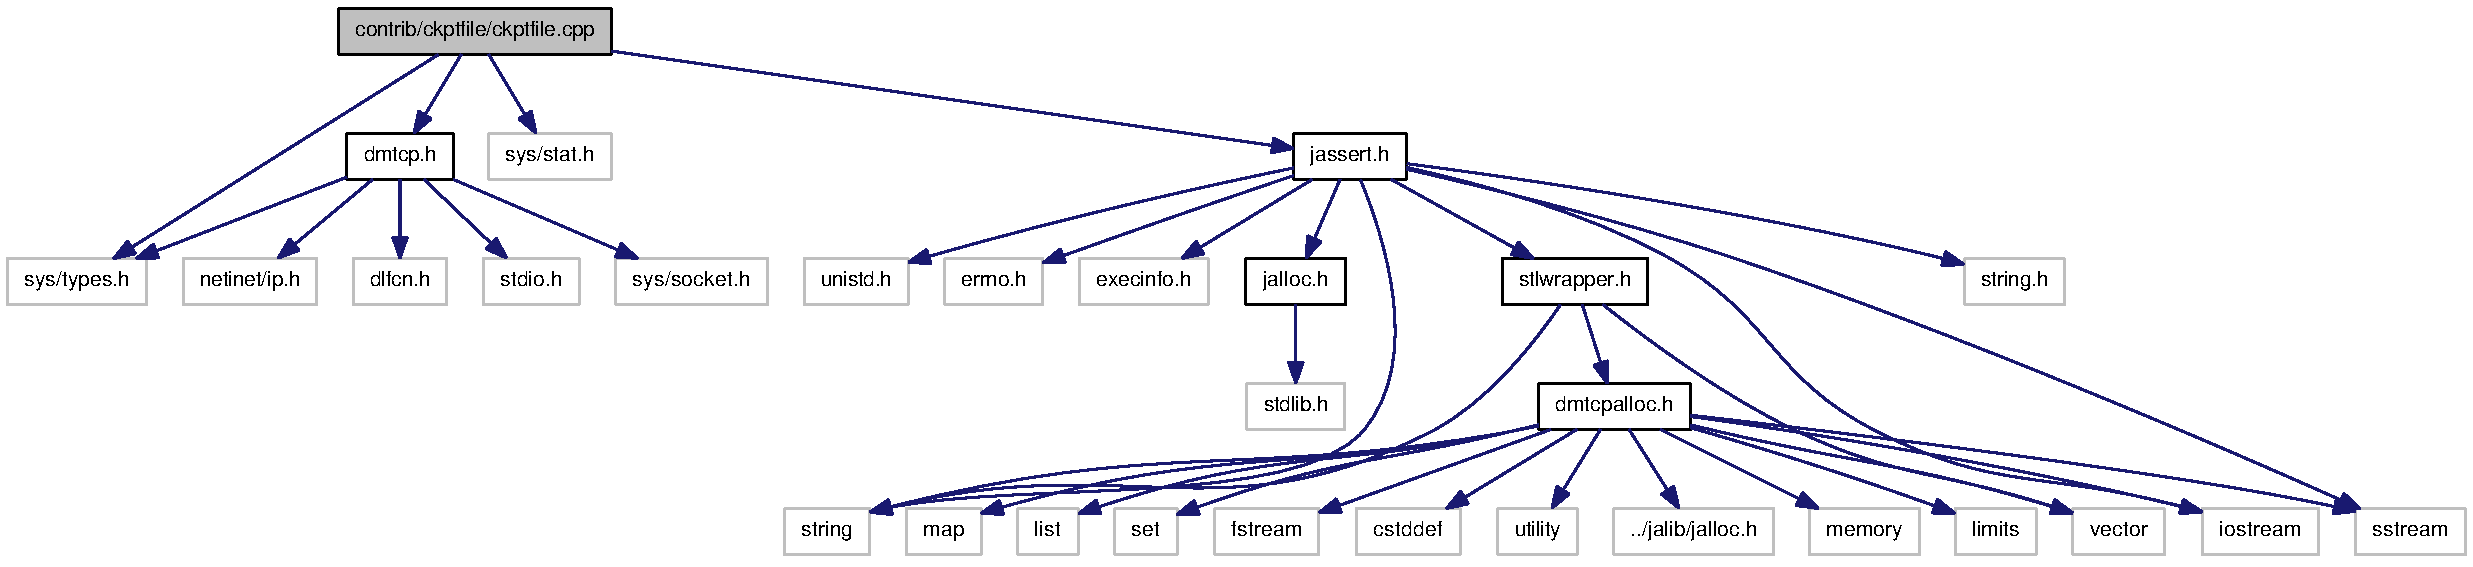
\includegraphics[width=420pt]{ckptfile_8cpp__incl}
\end{center}
\end{figure}
\subsection*{関数}
\begin{DoxyCompactItemize}
\item 
int \hyperlink{ckptfile_8cpp_ac01d5210970c9ed06aea0ee4da8a8ac0}{dmtcp\_\-must\_\-ckpt\_\-file} (const char $\ast$abspath)
\item 
void \hyperlink{ckptfile_8cpp_a84d40a7c26ba3d208cfa82d35d270eb9}{dmtcp\_\-get\_\-new\_\-file\_\-path} (const char $\ast$abspath, const char $\ast$cwd, char $\ast$newpath)
\item 
void \hyperlink{ckptfile_8cpp_a64b399d462bbbe394a56f94418f2d27a}{dmtcp\_\-event\_\-hook} (\hyperlink{dmtcp_8h_a1a2facd3d07dcfbe546435a70edb61ac}{DmtcpEvent\_\-t} event, \hyperlink{union__DmtcpEventData__t}{DmtcpEventData\_\-t} $\ast$data)
\end{DoxyCompactItemize}


\subsection{関数}
\hypertarget{ckptfile_8cpp_a64b399d462bbbe394a56f94418f2d27a}{
\index{ckptfile.cpp@{ckptfile.cpp}!dmtcp\_\-event\_\-hook@{dmtcp\_\-event\_\-hook}}
\index{dmtcp\_\-event\_\-hook@{dmtcp\_\-event\_\-hook}!ckptfile.cpp@{ckptfile.cpp}}
\subsubsection[{dmtcp\_\-event\_\-hook}]{\setlength{\rightskip}{0pt plus 5cm}void dmtcp\_\-event\_\-hook ({\bf DmtcpEvent\_\-t} {\em event}, \/  {\bf DmtcpEventData\_\-t} $\ast$ {\em data})}}
\label{ckptfile_8cpp_a64b399d462bbbe394a56f94418f2d27a}


呼出しグラフ:\nopagebreak
\begin{figure}[H]
\begin{center}
\leavevmode
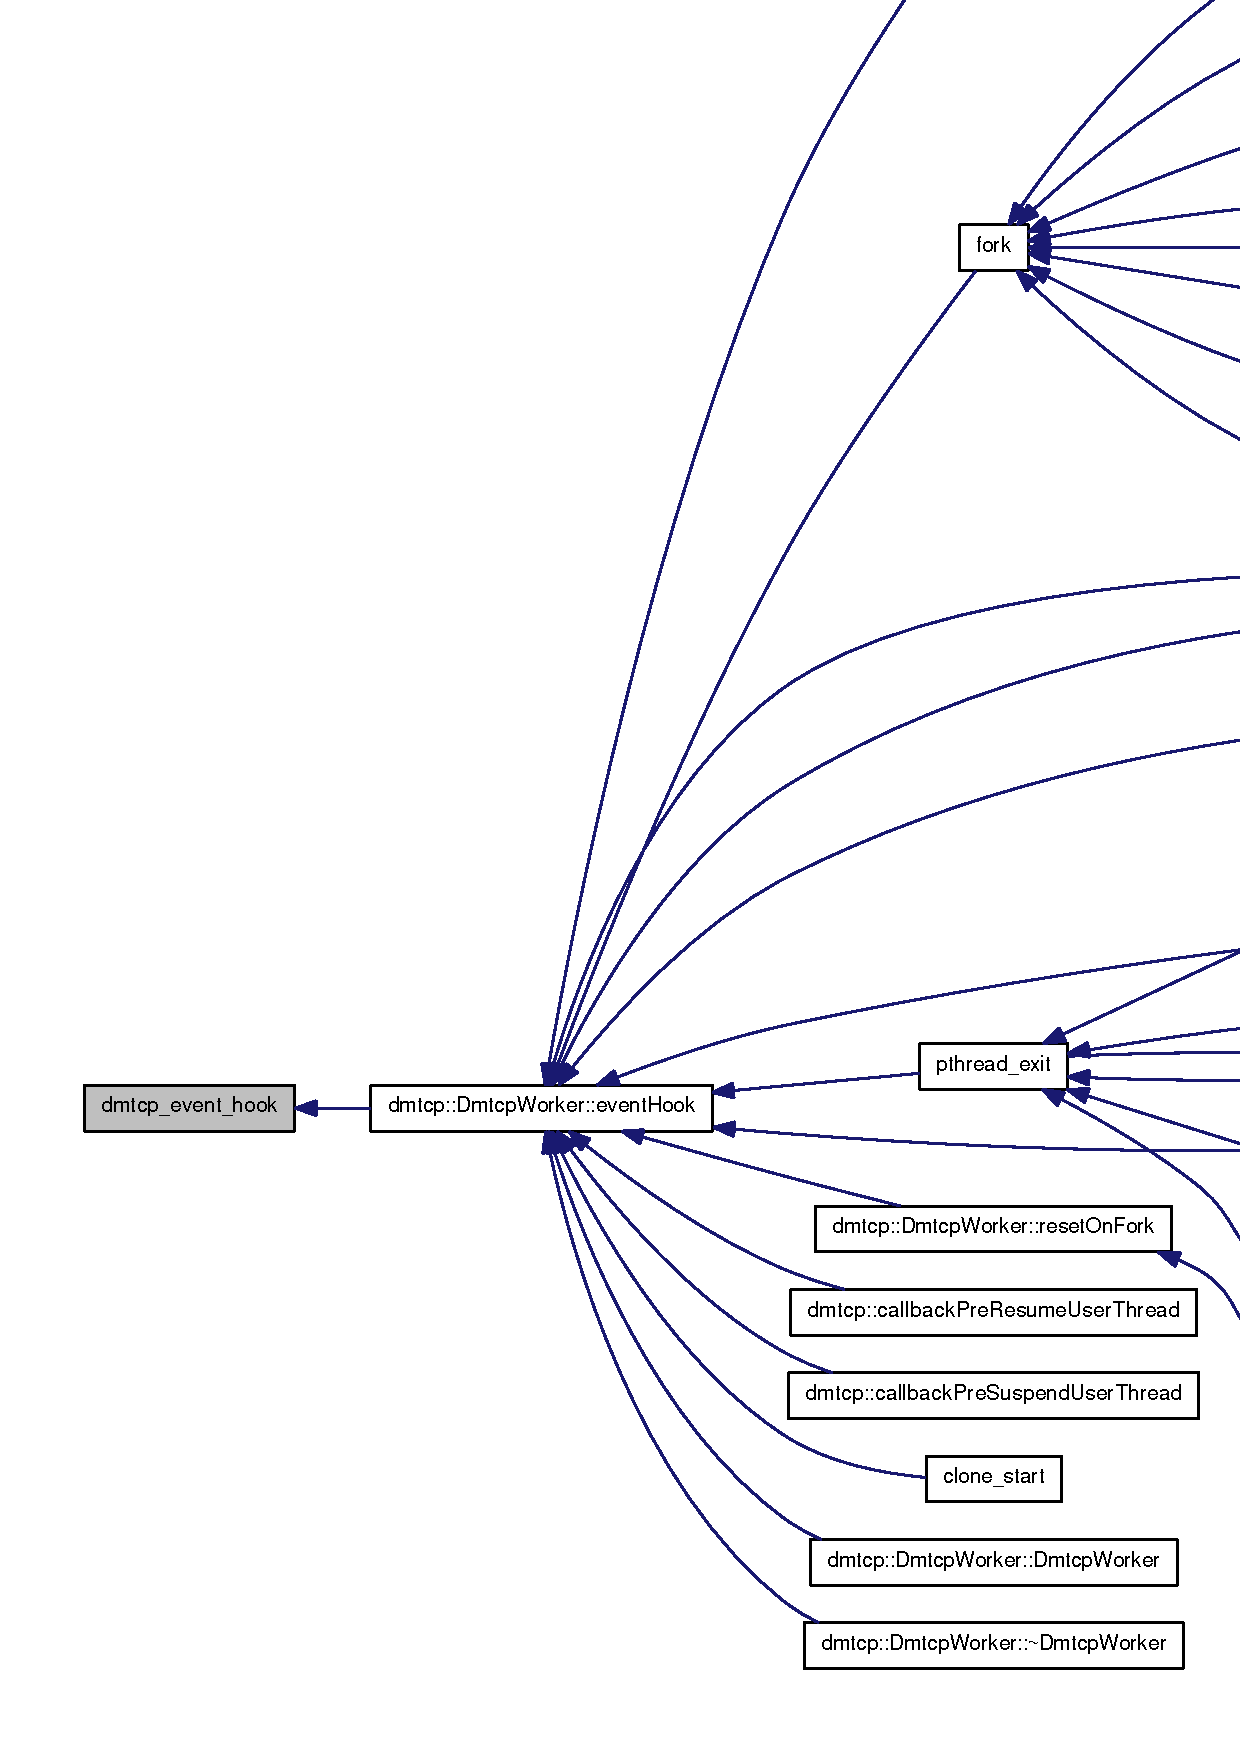
\includegraphics[width=420pt]{ckptfile_8cpp_a64b399d462bbbe394a56f94418f2d27a_icgraph}
\end{center}
\end{figure}
\hypertarget{ckptfile_8cpp_a84d40a7c26ba3d208cfa82d35d270eb9}{
\index{ckptfile.cpp@{ckptfile.cpp}!dmtcp\_\-get\_\-new\_\-file\_\-path@{dmtcp\_\-get\_\-new\_\-file\_\-path}}
\index{dmtcp\_\-get\_\-new\_\-file\_\-path@{dmtcp\_\-get\_\-new\_\-file\_\-path}!ckptfile.cpp@{ckptfile.cpp}}
\subsubsection[{dmtcp\_\-get\_\-new\_\-file\_\-path}]{\setlength{\rightskip}{0pt plus 5cm}void dmtcp\_\-get\_\-new\_\-file\_\-path (const char $\ast$ {\em abspath}, \/  const char $\ast$ {\em cwd}, \/  char $\ast$ {\em newpath})}}
\label{ckptfile_8cpp_a84d40a7c26ba3d208cfa82d35d270eb9}
\hypertarget{ckptfile_8cpp_ac01d5210970c9ed06aea0ee4da8a8ac0}{
\index{ckptfile.cpp@{ckptfile.cpp}!dmtcp\_\-must\_\-ckpt\_\-file@{dmtcp\_\-must\_\-ckpt\_\-file}}
\index{dmtcp\_\-must\_\-ckpt\_\-file@{dmtcp\_\-must\_\-ckpt\_\-file}!ckptfile.cpp@{ckptfile.cpp}}
\subsubsection[{dmtcp\_\-must\_\-ckpt\_\-file}]{\setlength{\rightskip}{0pt plus 5cm}int dmtcp\_\-must\_\-ckpt\_\-file (const char $\ast$ {\em abspath})}}
\label{ckptfile_8cpp_ac01d5210970c9ed06aea0ee4da8a8ac0}


呼出しグラフ:\nopagebreak
\begin{figure}[H]
\begin{center}
\leavevmode
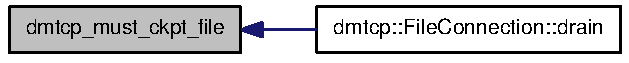
\includegraphics[width=169pt]{ckptfile_8cpp_ac01d5210970c9ed06aea0ee4da8a8ac0_icgraph}
\end{center}
\end{figure}

\hypertarget{ib2tcp_8cpp}{
\section{contrib/ib2tcp/ib2tcp.cpp}
\label{ib2tcp_8cpp}\index{contrib/ib2tcp/ib2tcp.cpp@{contrib/ib2tcp/ib2tcp.cpp}}
}
{\ttfamily \#include $<$infiniband/verbs.h$>$}\par
{\ttfamily \#include $<$linux/types.h$>$}\par
{\ttfamily \#include $<$sys/types.h$>$}\par
{\ttfamily \#include $<$fcntl.h$>$}\par
{\ttfamily \#include $<$assert.h$>$}\par
{\ttfamily \#include $<$stdlib.h$>$}\par
{\ttfamily \#include $<$stdbool.h$>$}\par
{\ttfamily \#include $<$stdio.h$>$}\par
{\ttfamily \#include $<$string.h$>$}\par
{\ttfamily \#include $<$pthread.h$>$}\par
{\ttfamily \#include $<$errno.h$>$}\par
{\ttfamily \#include $<$semaphore.h$>$}\par
{\ttfamily \#include $<$sys/socket.h$>$}\par
{\ttfamily \#include $<$netinet/in.h$>$}\par
{\ttfamily \#include $<$arpa/inet.h$>$}\par
{\ttfamily \#include $<$queue$>$}\par
{\ttfamily \#include \char`\"{}dmtcp.h\char`\"{}}\par
{\ttfamily \#include \char`\"{}dmtcpalloc.h\char`\"{}}\par
{\ttfamily \#include \char`\"{}util.h\char`\"{}}\par
{\ttfamily \#include \char`\"{}jsocket.h\char`\"{}}\par
{\ttfamily \#include \char`\"{}jassert.h\char`\"{}}\par
{\ttfamily \#include \char`\"{}ib2tcp.h\char`\"{}}\par
{\ttfamily \#include \char`\"{}ibwrappers.h\char`\"{}}\par
ib2tcp.cppのインクルード依存関係図\nopagebreak
\begin{figure}[H]
\begin{center}
\leavevmode
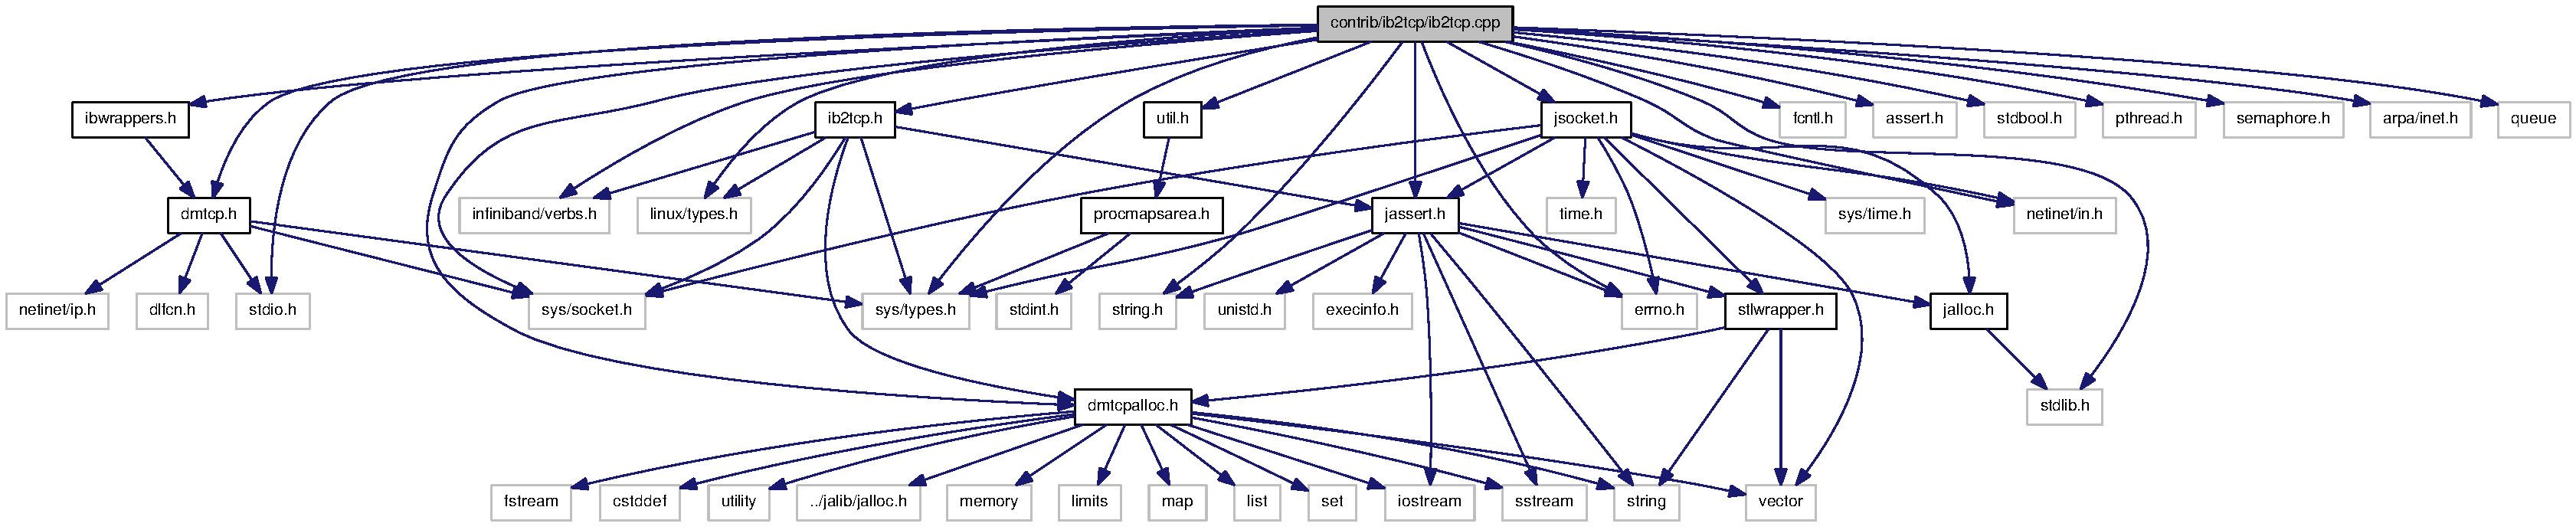
\includegraphics[width=420pt]{ib2tcp_8cpp__incl}
\end{center}
\end{figure}
\subsection*{関数}
\begin{DoxyCompactItemize}
\item 
void \hyperlink{ib2tcp_8cpp_a64b399d462bbbe394a56f94418f2d27a}{dmtcp\_\-event\_\-hook} (\hyperlink{dmtcp_8h_a1a2facd3d07dcfbe546435a70edb61ac}{DmtcpEvent\_\-t} event, \hyperlink{union__DmtcpEventData__t}{DmtcpEventData\_\-t} $\ast$data)
\end{DoxyCompactItemize}
\subsection*{変数}
\begin{DoxyCompactItemize}
\item 
\hyperlink{classdmtcp_1_1vector}{vector}$<$ \hyperlink{classdmtcp_1_1IB__WR}{IB\_\-WR}$<$ struct ibv\_\-send\_\-wr $>$ $\ast$ $>$ \hyperlink{ib2tcp_8cpp_a76e4f55fe1e6e0de2b85e891f0448f2c}{sendQueue}
\item 
\hyperlink{classdmtcp_1_1map}{map}$<$ \hyperlink{classdmtcp_1_1IB__QP}{IB\_\-QP} $\ast$, \hyperlink{classdmtcp_1_1vector}{vector}$<$ \hyperlink{classdmtcp_1_1IB__WR}{IB\_\-WR}$<$ struct ibv\_\-recv\_\-wr $>$ $\ast$ $>$ $>$ \hyperlink{ib2tcp_8cpp_a7a7c095eccdf4197993981f614523119}{recvQueue}
\item 
\hyperlink{classdmtcp_1_1map}{map}$<$ struct ibv\_\-srq $\ast$, \hyperlink{classdmtcp_1_1vector}{vector}$<$ \hyperlink{classdmtcp_1_1IB__WR}{IB\_\-WR}$<$ struct ibv\_\-recv\_\-wr $>$ $\ast$ $>$ $>$ \hyperlink{ib2tcp_8cpp_a9dbf6bef6ea167764d33cc36b724c229}{srecvQueue}
\item 
\hyperlink{classdmtcp_1_1map}{map}$<$ \hyperlink{classdmtcp_1_1IB__QP}{IB\_\-QP} $\ast$, int $>$ \hyperlink{ib2tcp_8cpp_acc8e06a5e5630b51450aa463a69e7dd2}{qpToFd}
\item 
\hyperlink{classdmtcp_1_1map}{map}$<$ int, \hyperlink{classdmtcp_1_1IB__QP}{IB\_\-QP} $\ast$ $>$ \hyperlink{ib2tcp_8cpp_a8aa5b21222d66de1ebc5b56b9aa993e2}{fdToQP}
\item 
\hyperlink{classdmtcp_1_1vector}{vector}$<$ int $>$ \hyperlink{ib2tcp_8cpp_a79ac9994b44108a6ff259354547871e0}{socks}
\item 
\hyperlink{classdmtcp_1_1map}{map}$<$ uint32\_\-t, \hyperlink{classdmtcp_1_1IB__QP}{IB\_\-QP} $\ast$ $>$ \hyperlink{ib2tcp_8cpp_a72c426f5383de0a140ac4775d69d4a94}{queuePairs}
\item 
\hyperlink{classdmtcp_1_1map}{map}$<$ struct ibv\_\-cq $\ast$, \hyperlink{classdmtcp_1_1vector}{vector}$<$ struct ibv\_\-wc $>$ $>$ \hyperlink{ib2tcp_8cpp_a7825f0d024bb777860bfe4d0c8e72411}{compQueue}
\item 
\hyperlink{classdmtcp_1_1map}{map}$<$ struct ibv\_\-cq $\ast$, sem\_\-t $\ast$ $>$ \hyperlink{ib2tcp_8cpp_ac09d1f30cc037ab14968f4a47dd44c32}{compQueueSema}
\item 
sem\_\-t \hyperlink{ib2tcp_8cpp_ae939f55e536d953e9d6dbed0ed976340}{sem\_\-queue}
\item 
\hyperlink{classjalib_1_1JServerSocket}{jalib::JServerSocket} \hyperlink{ib2tcp_8cpp_a1272d4970ec8542bb04558a885256d6e}{listenSock} (-\/1)
\item 
pthread\_\-t \hyperlink{ib2tcp_8cpp_a09dbe53d7c6f96282a2493f2cfb3f86a}{sendTh} = -\/1
\item 
pthread\_\-t \hyperlink{ib2tcp_8cpp_a5eb571e07025b4d6c01593d07404f3ae}{recvTh} = -\/1
\item 
int \hyperlink{ib2tcp_8cpp_a4eb6e16937eb7b9a7a35540e7a49710d}{isVirtIB} = 0
\end{DoxyCompactItemize}


\subsection{関数}
\hypertarget{ib2tcp_8cpp_a64b399d462bbbe394a56f94418f2d27a}{
\index{ib2tcp.cpp@{ib2tcp.cpp}!dmtcp\_\-event\_\-hook@{dmtcp\_\-event\_\-hook}}
\index{dmtcp\_\-event\_\-hook@{dmtcp\_\-event\_\-hook}!ib2tcp.cpp@{ib2tcp.cpp}}
\subsubsection[{dmtcp\_\-event\_\-hook}]{\setlength{\rightskip}{0pt plus 5cm}void dmtcp\_\-event\_\-hook ({\bf DmtcpEvent\_\-t} {\em event}, \/  {\bf DmtcpEventData\_\-t} $\ast$ {\em data})}}
\label{ib2tcp_8cpp_a64b399d462bbbe394a56f94418f2d27a}


関数の呼び出しグラフ:\nopagebreak
\begin{figure}[H]
\begin{center}
\leavevmode
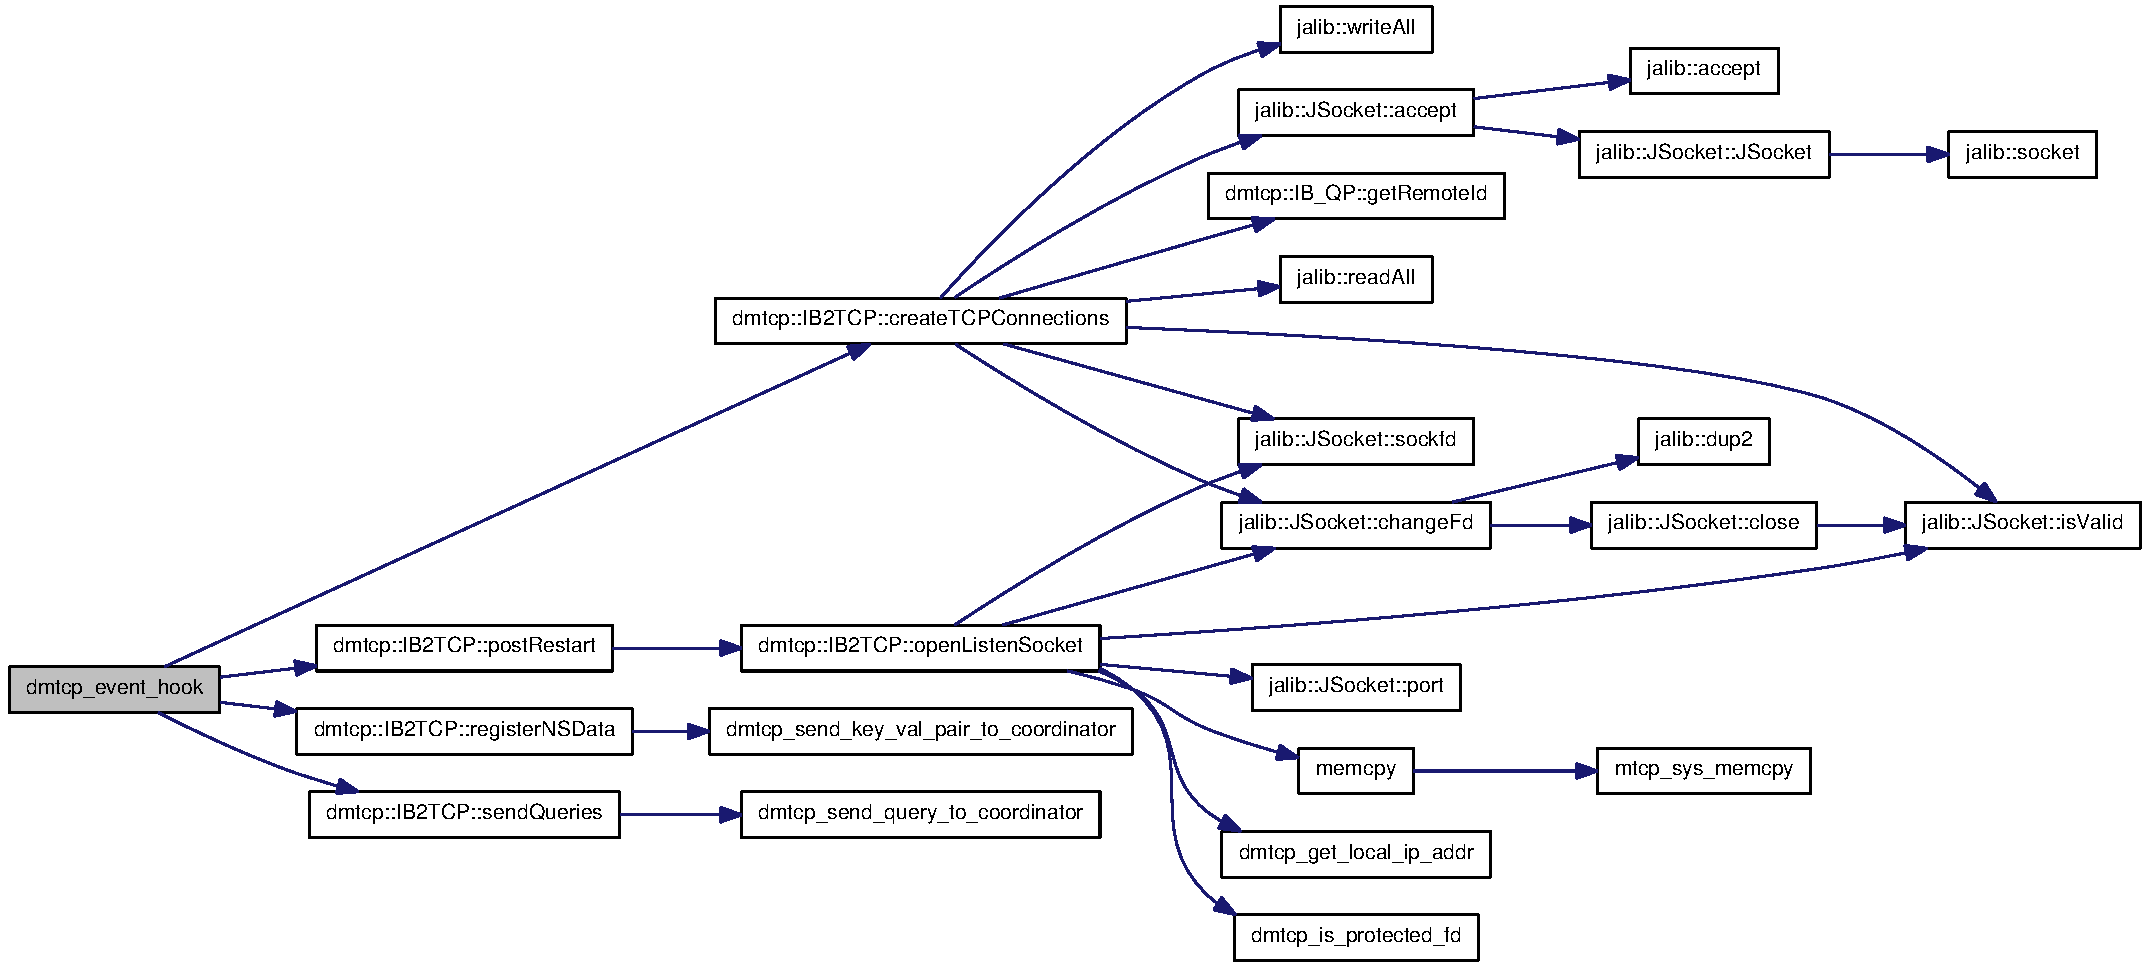
\includegraphics[width=420pt]{ib2tcp_8cpp_a64b399d462bbbe394a56f94418f2d27a_cgraph}
\end{center}
\end{figure}


\subsection{変数}
\hypertarget{ib2tcp_8cpp_a7825f0d024bb777860bfe4d0c8e72411}{
\index{ib2tcp.cpp@{ib2tcp.cpp}!compQueue@{compQueue}}
\index{compQueue@{compQueue}!ib2tcp.cpp@{ib2tcp.cpp}}
\subsubsection[{compQueue}]{\setlength{\rightskip}{0pt plus 5cm}{\bf map}$<$struct ibv\_\-cq$\ast$, {\bf vector}$<$struct ibv\_\-wc$>$ $>$ {\bf compQueue}}}
\label{ib2tcp_8cpp_a7825f0d024bb777860bfe4d0c8e72411}
\hypertarget{ib2tcp_8cpp_ac09d1f30cc037ab14968f4a47dd44c32}{
\index{ib2tcp.cpp@{ib2tcp.cpp}!compQueueSema@{compQueueSema}}
\index{compQueueSema@{compQueueSema}!ib2tcp.cpp@{ib2tcp.cpp}}
\subsubsection[{compQueueSema}]{\setlength{\rightskip}{0pt plus 5cm}{\bf map}$<$struct ibv\_\-cq$\ast$, sem\_\-t $\ast$$>$ {\bf compQueueSema}}}
\label{ib2tcp_8cpp_ac09d1f30cc037ab14968f4a47dd44c32}
\hypertarget{ib2tcp_8cpp_a8aa5b21222d66de1ebc5b56b9aa993e2}{
\index{ib2tcp.cpp@{ib2tcp.cpp}!fdToQP@{fdToQP}}
\index{fdToQP@{fdToQP}!ib2tcp.cpp@{ib2tcp.cpp}}
\subsubsection[{fdToQP}]{\setlength{\rightskip}{0pt plus 5cm}{\bf map}$<$int, {\bf IB\_\-QP}$\ast$$>$ {\bf fdToQP}}}
\label{ib2tcp_8cpp_a8aa5b21222d66de1ebc5b56b9aa993e2}
\hypertarget{ib2tcp_8cpp_a4eb6e16937eb7b9a7a35540e7a49710d}{
\index{ib2tcp.cpp@{ib2tcp.cpp}!isVirtIB@{isVirtIB}}
\index{isVirtIB@{isVirtIB}!ib2tcp.cpp@{ib2tcp.cpp}}
\subsubsection[{isVirtIB}]{\setlength{\rightskip}{0pt plus 5cm}int {\bf isVirtIB} = 0}}
\label{ib2tcp_8cpp_a4eb6e16937eb7b9a7a35540e7a49710d}
\hypertarget{ib2tcp_8cpp_a1272d4970ec8542bb04558a885256d6e}{
\index{ib2tcp.cpp@{ib2tcp.cpp}!listenSock@{listenSock}}
\index{listenSock@{listenSock}!ib2tcp.cpp@{ib2tcp.cpp}}
\subsubsection[{listenSock}]{\setlength{\rightskip}{0pt plus 5cm}{\bf jalib::JServerSocket} {\bf listenSock}(-\/1)}}
\label{ib2tcp_8cpp_a1272d4970ec8542bb04558a885256d6e}
\hypertarget{ib2tcp_8cpp_acc8e06a5e5630b51450aa463a69e7dd2}{
\index{ib2tcp.cpp@{ib2tcp.cpp}!qpToFd@{qpToFd}}
\index{qpToFd@{qpToFd}!ib2tcp.cpp@{ib2tcp.cpp}}
\subsubsection[{qpToFd}]{\setlength{\rightskip}{0pt plus 5cm}{\bf map}$<${\bf IB\_\-QP}$\ast$, int$>$ {\bf qpToFd}}}
\label{ib2tcp_8cpp_acc8e06a5e5630b51450aa463a69e7dd2}
\hypertarget{ib2tcp_8cpp_a72c426f5383de0a140ac4775d69d4a94}{
\index{ib2tcp.cpp@{ib2tcp.cpp}!queuePairs@{queuePairs}}
\index{queuePairs@{queuePairs}!ib2tcp.cpp@{ib2tcp.cpp}}
\subsubsection[{queuePairs}]{\setlength{\rightskip}{0pt plus 5cm}{\bf map}$<$uint32\_\-t, {\bf IB\_\-QP}$\ast$$>$ {\bf queuePairs}}}
\label{ib2tcp_8cpp_a72c426f5383de0a140ac4775d69d4a94}
\hypertarget{ib2tcp_8cpp_a7a7c095eccdf4197993981f614523119}{
\index{ib2tcp.cpp@{ib2tcp.cpp}!recvQueue@{recvQueue}}
\index{recvQueue@{recvQueue}!ib2tcp.cpp@{ib2tcp.cpp}}
\subsubsection[{recvQueue}]{\setlength{\rightskip}{0pt plus 5cm}{\bf map}$<${\bf IB\_\-QP}$\ast$, {\bf vector}$<${\bf IB\_\-WR}$<$struct ibv\_\-recv\_\-wr$>$$\ast$ $>$ $>$ {\bf recvQueue}}}
\label{ib2tcp_8cpp_a7a7c095eccdf4197993981f614523119}
\hypertarget{ib2tcp_8cpp_a5eb571e07025b4d6c01593d07404f3ae}{
\index{ib2tcp.cpp@{ib2tcp.cpp}!recvTh@{recvTh}}
\index{recvTh@{recvTh}!ib2tcp.cpp@{ib2tcp.cpp}}
\subsubsection[{recvTh}]{\setlength{\rightskip}{0pt plus 5cm}pthread\_\-t {\bf recvTh} = -\/1}}
\label{ib2tcp_8cpp_a5eb571e07025b4d6c01593d07404f3ae}
\hypertarget{ib2tcp_8cpp_ae939f55e536d953e9d6dbed0ed976340}{
\index{ib2tcp.cpp@{ib2tcp.cpp}!sem\_\-queue@{sem\_\-queue}}
\index{sem\_\-queue@{sem\_\-queue}!ib2tcp.cpp@{ib2tcp.cpp}}
\subsubsection[{sem\_\-queue}]{\setlength{\rightskip}{0pt plus 5cm}sem\_\-t {\bf sem\_\-queue}}}
\label{ib2tcp_8cpp_ae939f55e536d953e9d6dbed0ed976340}
\hypertarget{ib2tcp_8cpp_a76e4f55fe1e6e0de2b85e891f0448f2c}{
\index{ib2tcp.cpp@{ib2tcp.cpp}!sendQueue@{sendQueue}}
\index{sendQueue@{sendQueue}!ib2tcp.cpp@{ib2tcp.cpp}}
\subsubsection[{sendQueue}]{\setlength{\rightskip}{0pt plus 5cm}{\bf vector}$<${\bf IB\_\-WR}$<$struct ibv\_\-send\_\-wr$>$$\ast$ $>$ {\bf sendQueue}}}
\label{ib2tcp_8cpp_a76e4f55fe1e6e0de2b85e891f0448f2c}
\hypertarget{ib2tcp_8cpp_a09dbe53d7c6f96282a2493f2cfb3f86a}{
\index{ib2tcp.cpp@{ib2tcp.cpp}!sendTh@{sendTh}}
\index{sendTh@{sendTh}!ib2tcp.cpp@{ib2tcp.cpp}}
\subsubsection[{sendTh}]{\setlength{\rightskip}{0pt plus 5cm}pthread\_\-t {\bf sendTh} = -\/1}}
\label{ib2tcp_8cpp_a09dbe53d7c6f96282a2493f2cfb3f86a}
\hypertarget{ib2tcp_8cpp_a79ac9994b44108a6ff259354547871e0}{
\index{ib2tcp.cpp@{ib2tcp.cpp}!socks@{socks}}
\index{socks@{socks}!ib2tcp.cpp@{ib2tcp.cpp}}
\subsubsection[{socks}]{\setlength{\rightskip}{0pt plus 5cm}{\bf vector}$<$int$>$ {\bf socks}}}
\label{ib2tcp_8cpp_a79ac9994b44108a6ff259354547871e0}
\hypertarget{ib2tcp_8cpp_a9dbf6bef6ea167764d33cc36b724c229}{
\index{ib2tcp.cpp@{ib2tcp.cpp}!srecvQueue@{srecvQueue}}
\index{srecvQueue@{srecvQueue}!ib2tcp.cpp@{ib2tcp.cpp}}
\subsubsection[{srecvQueue}]{\setlength{\rightskip}{0pt plus 5cm}{\bf map}$<$struct ibv\_\-srq$\ast$, {\bf vector}$<${\bf IB\_\-WR}$<$struct ibv\_\-recv\_\-wr$>$$\ast$ $>$ $>$ {\bf srecvQueue}}}
\label{ib2tcp_8cpp_a9dbf6bef6ea167764d33cc36b724c229}

\hypertarget{ib2tcp_8h}{
\section{contrib/ib2tcp/ib2tcp.h}
\label{ib2tcp_8h}\index{contrib/ib2tcp/ib2tcp.h@{contrib/ib2tcp/ib2tcp.h}}
}
{\ttfamily \#include $<$infiniband/verbs.h$>$}\par
{\ttfamily \#include $<$linux/types.h$>$}\par
{\ttfamily \#include $<$sys/types.h$>$}\par
{\ttfamily \#include $<$sys/socket.h$>$}\par
{\ttfamily \#include \char`\"{}dmtcpalloc.h\char`\"{}}\par
{\ttfamily \#include \char`\"{}jassert.h\char`\"{}}\par
ib2tcp.hのインクルード依存関係図\nopagebreak
\begin{figure}[H]
\begin{center}
\leavevmode
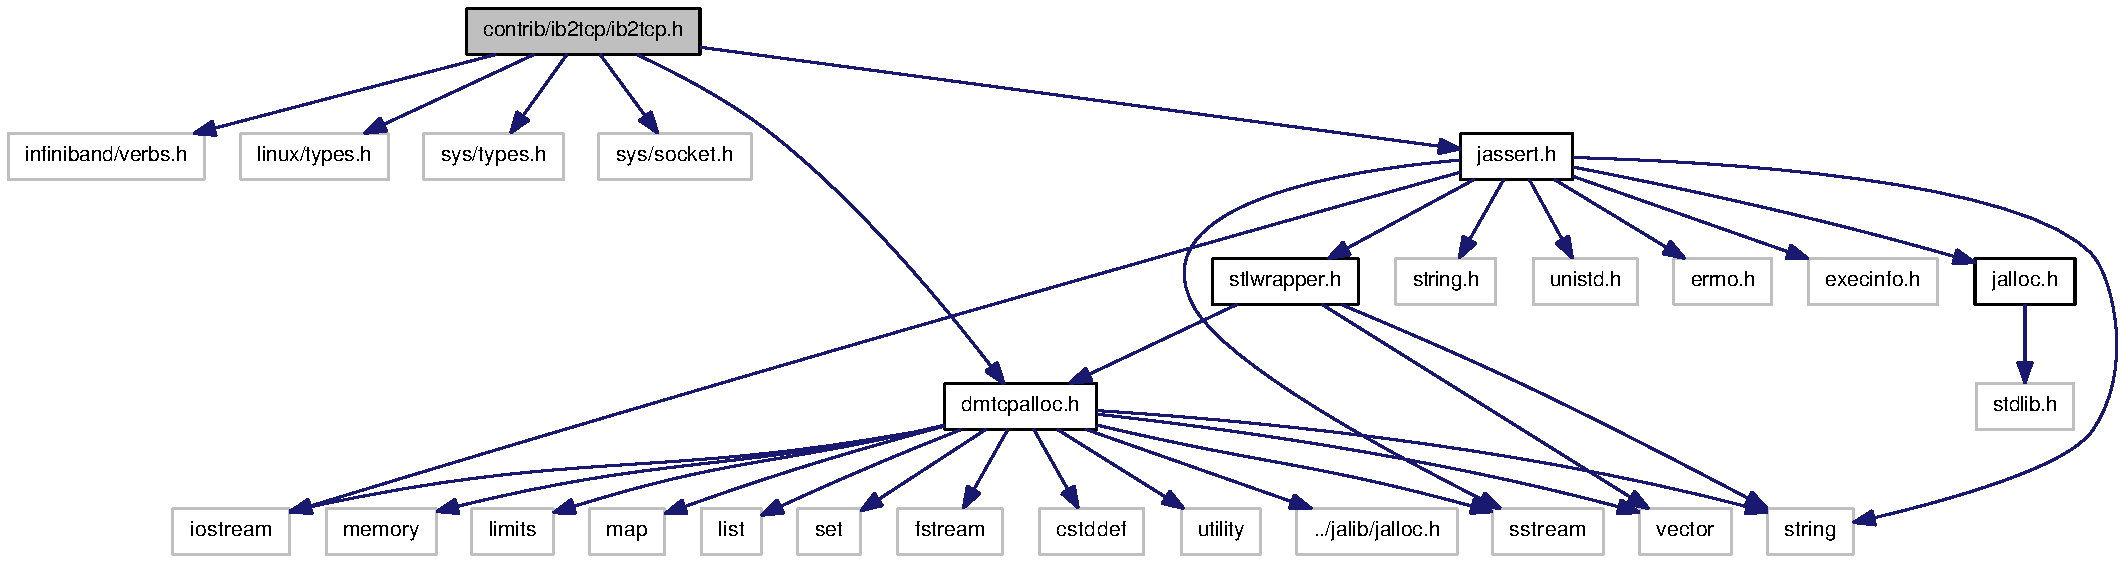
\includegraphics[width=420pt]{ib2tcp_8h__incl}
\end{center}
\end{figure}
このグラフは、どのファイルから直接、間接的にインクルードされているかを示しています。\nopagebreak
\begin{figure}[H]
\begin{center}
\leavevmode
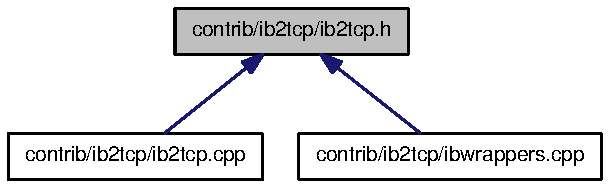
\includegraphics[width=164pt]{ib2tcp_8h__dep__incl}
\end{center}
\end{figure}
\subsection*{構成}
\begin{DoxyCompactItemize}
\item 
struct \hyperlink{structdmtcp_1_1IB__QId}{dmtcp::IB\_\-QId}
\item 
class \hyperlink{classdmtcp_1_1IB__QP}{dmtcp::IB\_\-QP}
\item 
class \hyperlink{classdmtcp_1_1IB__WR}{dmtcp::IB\_\-WR$<$ WRType $>$}
\end{DoxyCompactItemize}
\subsection*{ネームスペース}
\begin{DoxyCompactItemize}
\item 
namespace \hyperlink{namespacedmtcp}{dmtcp}
\item 
namespace \hyperlink{namespacedmtcp_1_1IB2TCP}{dmtcp::IB2TCP}
\end{DoxyCompactItemize}
\subsection*{型定義}
\begin{DoxyCompactItemize}
\item 
typedef struct \hyperlink{structdmtcp_1_1IB__QId}{dmtcp::IB\_\-QId} \hyperlink{namespacedmtcp_afda193ac8c968524934458ded0a0e4e1}{dmtcp::IB\_\-QId}
\end{DoxyCompactItemize}
\subsection*{関数}
\begin{DoxyCompactItemize}
\item 
void \hyperlink{namespacedmtcp_1_1IB2TCP_af8a08acba9c8ea1a13aaae43b0c6b4bf}{dmtcp::IB2TCP::openListenSocket} ()
\item 
void \hyperlink{namespacedmtcp_1_1IB2TCP_a0c2e76163bc7ee8a0f26b9b7f6ee44a6}{dmtcp::IB2TCP::postRestart} ()
\item 
void \hyperlink{namespacedmtcp_1_1IB2TCP_a575398b2da4ed9e4b6f99867ecc01924}{dmtcp::IB2TCP::init} ()
\item 
void \hyperlink{namespacedmtcp_1_1IB2TCP_a7135d30f54a3256f2df60945165a5140}{dmtcp::IB2TCP::registerNSData} ()
\item 
void \hyperlink{namespacedmtcp_1_1IB2TCP_ab7ca35e64f6e99fb496d372a208d75be}{dmtcp::IB2TCP::sendQueries} ()
\item 
void \hyperlink{namespacedmtcp_1_1IB2TCP_adad4535261361aaa3e6076fdce3e98f0}{dmtcp::IB2TCP::createTCPConnections} ()
\item 
void \hyperlink{namespacedmtcp_1_1IB2TCP_a3be272d6c87725bb03f140107b06d3a9}{dmtcp::IB2TCP::doRecvMsg} (int fd)
\item 
void \hyperlink{namespacedmtcp_1_1IB2TCP_a6b42cdfaa01dc1e83d7a3f20c6ee301b}{dmtcp::IB2TCP::doSendMsg} ()
\item 
void \hyperlink{namespacedmtcp_1_1IB2TCP_ae34871060ae603e2ae724bb87d8a1cc0}{dmtcp::IB2TCP::regQIdToListenAddrWithCoord} (IB\_\-QId qid)
\item 
void \hyperlink{namespacedmtcp_1_1IB2TCP_a0ece616f6840ce364bd0e0639a3addb1}{dmtcp::IB2TCP::createQP} (struct ibv\_\-qp $\ast$qp, struct ibv\_\-qp\_\-init\_\-attr $\ast$qp\_\-init\_\-attr)
\item 
void \hyperlink{namespacedmtcp_1_1IB2TCP_a2178efc9b005ff70f306bb53963b1b4c}{dmtcp::IB2TCP::modifyQP} (struct ibv\_\-qp $\ast$qp, struct ibv\_\-qp\_\-attr $\ast$attr, int mask)
\item 
int \hyperlink{namespacedmtcp_1_1IB2TCP_ade9ea4f23b593dda51c14dd45dcb9d3a}{dmtcp::IB2TCP::postSend} (struct ibv\_\-qp $\ast$qp, struct ibv\_\-send\_\-wr $\ast$wr, struct ibv\_\-send\_\-wr $\ast$$\ast$bad\_\-wr)
\item 
int \hyperlink{namespacedmtcp_1_1IB2TCP_a60a304f9ea7bd224a81d3c32a90e75ec}{dmtcp::IB2TCP::postRecv} (struct ibv\_\-qp $\ast$qp, struct ibv\_\-recv\_\-wr $\ast$wr, struct ibv\_\-recv\_\-wr $\ast$$\ast$bad\_\-wr)
\item 
int \hyperlink{namespacedmtcp_1_1IB2TCP_a0c774bc7f3e6fcf90291fd8cfbac9376}{dmtcp::IB2TCP::postSrqRecv} (struct ibv\_\-srq $\ast$srq, struct ibv\_\-recv\_\-wr $\ast$wr, struct ibv\_\-recv\_\-wr $\ast$$\ast$bad\_\-wr)
\item 
int \hyperlink{namespacedmtcp_1_1IB2TCP_a697b910ac51162756b1adc455bc620fd}{dmtcp::IB2TCP::pollCq} (struct ibv\_\-cq $\ast$cq, int num\_\-entries, struct ibv\_\-wc $\ast$wc)
\item 
int \hyperlink{namespacedmtcp_1_1IB2TCP_a505c1e6da6d5f920207c16297dab3d4d}{dmtcp::IB2TCP::postPollCq} (struct ibv\_\-cq $\ast$cq, int num\_\-entries, struct ibv\_\-wc $\ast$wc)
\item 
int \hyperlink{namespacedmtcp_1_1IB2TCP_a78cec0f57d84425d3a376269cc9871ba}{dmtcp::IB2TCP::req\_\-notify\_\-cq} (struct ibv\_\-cq $\ast$cq, int solicited\_\-only)
\item 
bool \hyperlink{namespacedmtcp_afc352ab11147b4aea54e054bd4d9d03d}{dmtcp::operator$<$} (\hyperlink{structdmtcp_1_1IB__QId}{IB\_\-QId} \&a, \hyperlink{structdmtcp_1_1IB__QId}{IB\_\-QId} \&b)
\item 
bool \hyperlink{namespacedmtcp_a650540c8e55de583ceef9d0a0d4efe63}{dmtcp::operator$>$} (\hyperlink{structdmtcp_1_1IB__QId}{IB\_\-QId} \&a, \hyperlink{structdmtcp_1_1IB__QId}{IB\_\-QId} \&b)
\item 
bool \hyperlink{namespacedmtcp_a7650477334e22827d746dcc83a7f8c80}{dmtcp::operator==} (\hyperlink{structdmtcp_1_1IB__QId}{IB\_\-QId} \&a, \hyperlink{structdmtcp_1_1IB__QId}{IB\_\-QId} \&b)
\item 
bool \hyperlink{namespacedmtcp_a4c5b65e3889d4002df277b79e63a9ba4}{dmtcp::operator!=} (\hyperlink{structdmtcp_1_1IB__QId}{IB\_\-QId} \&a, \hyperlink{structdmtcp_1_1IB__QId}{IB\_\-QId} \&b)
\end{DoxyCompactItemize}

\hypertarget{ibwrappers_8cpp}{
\section{contrib/ib2tcp/ibwrappers.cpp}
\label{ibwrappers_8cpp}\index{contrib/ib2tcp/ibwrappers.cpp@{contrib/ib2tcp/ibwrappers.cpp}}
}
{\ttfamily \#include $<$dlfcn.h$>$}\par
{\ttfamily \#include $<$stdio.h$>$}\par
{\ttfamily \#include $<$stdlib.h$>$}\par
{\ttfamily \#include $<$string.h$>$}\par
{\ttfamily \#include $<$sys/select.h$>$}\par
{\ttfamily \#include $<$sys/un.h$>$}\par
{\ttfamily \#include $<$arpa/inet.h$>$}\par
{\ttfamily \#include $<$pthread.h$>$}\par
{\ttfamily \#include $<$sys/types.h$>$}\par
{\ttfamily \#include $<$unistd.h$>$}\par
{\ttfamily \#include $<$errno.h$>$}\par
{\ttfamily \#include $<$infiniband/verbs.h$>$}\par
{\ttfamily \#include \char`\"{}dmtcp.h\char`\"{}}\par
{\ttfamily \#include \char`\"{}ib2tcp.h\char`\"{}}\par
{\ttfamily \#include \char`\"{}jassert.h\char`\"{}}\par
{\ttfamily \#include \char`\"{}ibwrappers.h\char`\"{}}\par
ibwrappers.cppのインクルード依存関係図\nopagebreak
\begin{figure}[H]
\begin{center}
\leavevmode
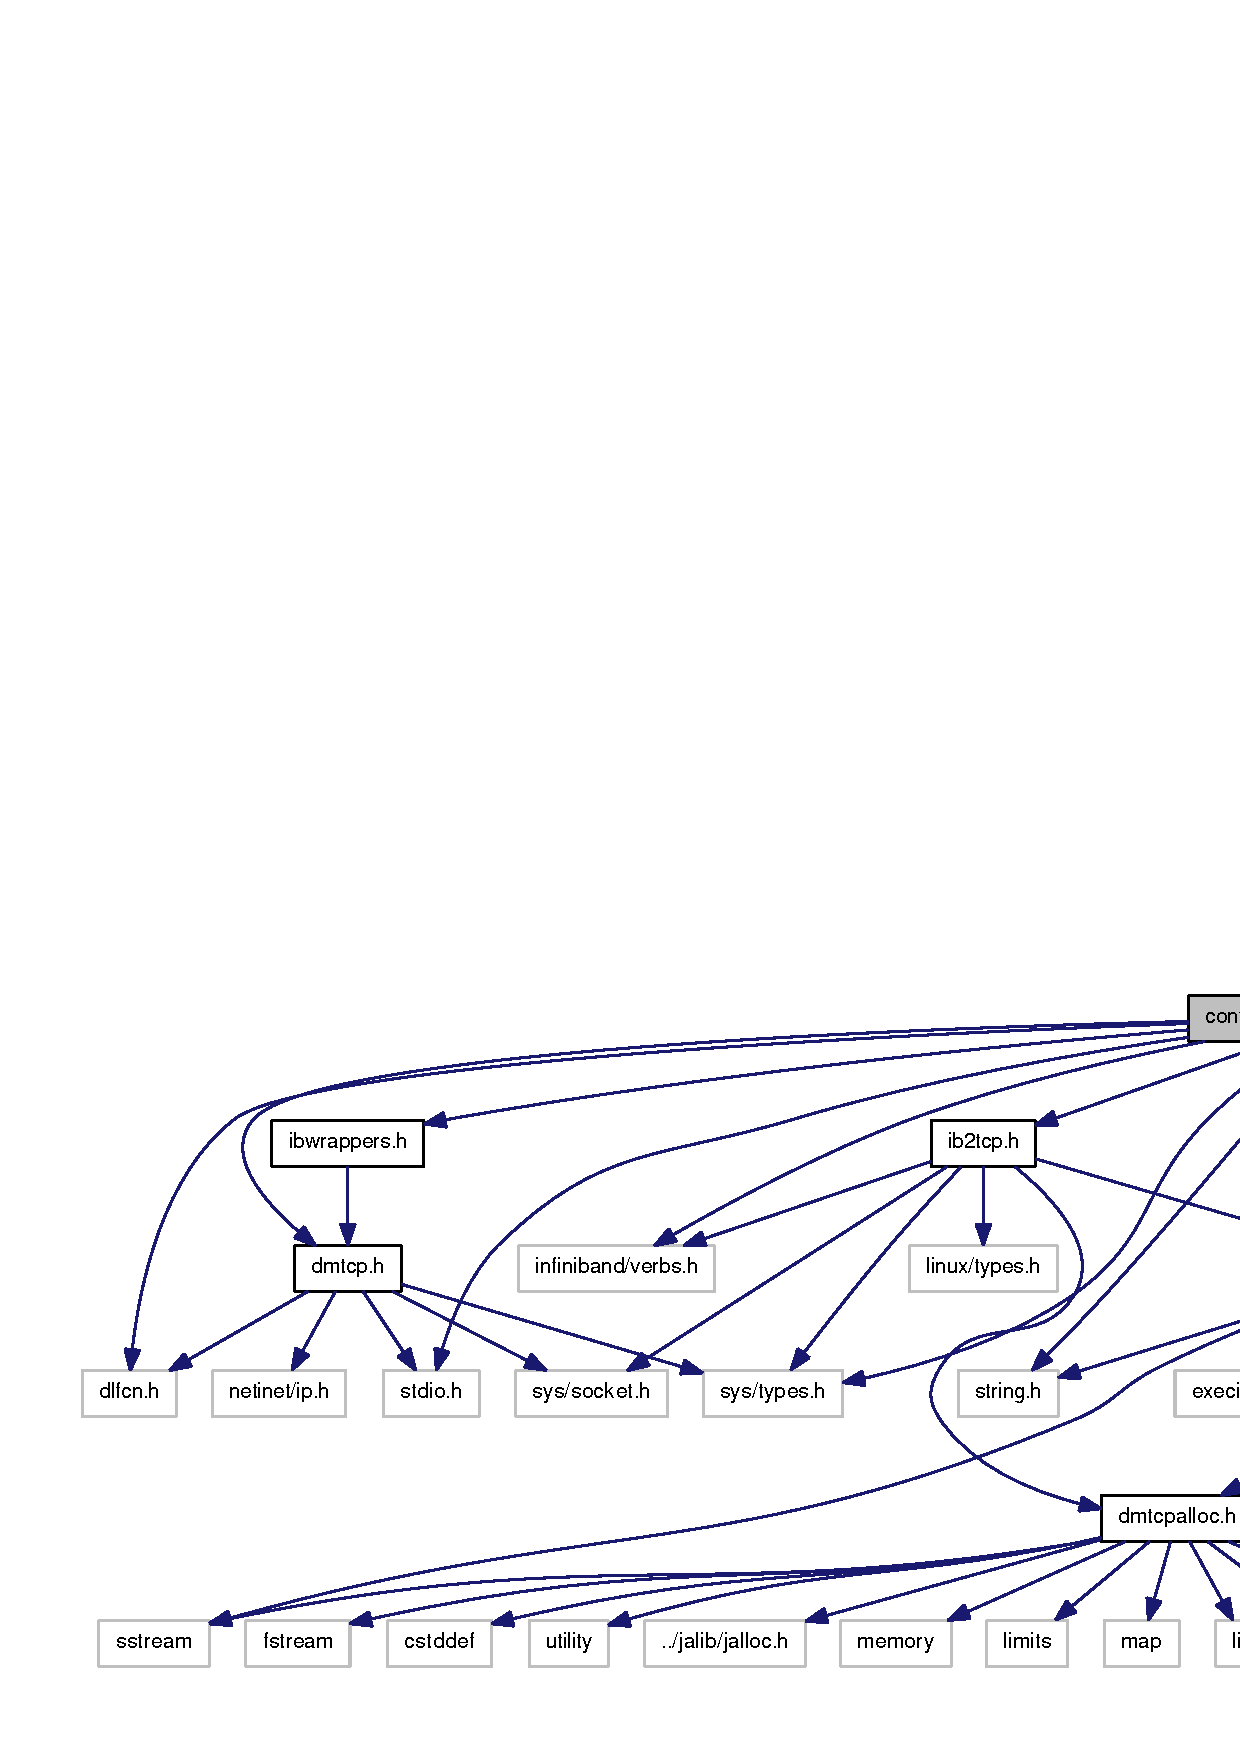
\includegraphics[width=420pt]{ibwrappers_8cpp__incl}
\end{center}
\end{figure}
\subsection*{マクロ定義}
\begin{DoxyCompactItemize}
\item 
\#define \hyperlink{ibwrappers_8cpp_a12dd28d5174849c4fbcf06f8ea4045cd}{DECL\_\-FPTR}(func)~static \_\-\_\-typeof\_\-\_\-(\&ib2t\_\-\#\#func) \_\-real\_\-ibv\_\-\#\#func = (\_\-\_\-typeof\_\-\_\-(\&ib2t\_\-\#\#func)) NULL
\item 
\#define \hyperlink{ibwrappers_8cpp_ab36b6479de561fc14ea76335f401ec2a}{UPDATE\_\-FUNC\_\-ADDR}(func, addr)
\end{DoxyCompactItemize}
\subsection*{関数}
\begin{DoxyCompactItemize}
\item 
\hyperlink{ibwrappers_8cpp_a746b91ba8102eb7525f6e264ab35d1cc}{DECL\_\-FPTR} (post\_\-recv)
\item 
\hyperlink{ibwrappers_8cpp_aedd7c41490ae971725181c53b229b7ce}{DECL\_\-FPTR} (post\_\-srq\_\-recv)
\item 
\hyperlink{ibwrappers_8cpp_a9492871aa0c64336abd5c9e042643246}{DECL\_\-FPTR} (post\_\-send)
\item 
\hyperlink{ibwrappers_8cpp_a0a6abd1ab839e028b6f083ac98e612ea}{DECL\_\-FPTR} (poll\_\-cq)
\item 
\hyperlink{ibwrappers_8cpp_a9884daa90775ad31af57efff2e4ef86c}{DECL\_\-FPTR} (req\_\-notify\_\-cq)
\item 
struct ibv\_\-context $\ast$ \hyperlink{ibwrappers_8cpp_a8e14823e543fe663dd0bffe6e05708cd}{ibv\_\-open\_\-device} (struct ibv\_\-device $\ast$dev)
\item 
struct ibv\_\-qp $\ast$ \hyperlink{ibwrappers_8cpp_a4d733171c73a340e292b66a91bd81401}{ibv\_\-create\_\-qp} (struct ibv\_\-pd $\ast$pd, struct ibv\_\-qp\_\-init\_\-attr $\ast$qp\_\-init\_\-attr)
\item 
int \hyperlink{ibwrappers_8cpp_a7775daa82f7e8814ead91b40dbd5eb95}{ibv\_\-modify\_\-qp} (struct ibv\_\-qp $\ast$qp, struct ibv\_\-qp\_\-attr $\ast$attr, int attr\_\-mask)
\item 
int \hyperlink{ibwrappers_8cpp_aa0fc78a4ee91da053d4d5be704223411}{ibv\_\-destroy\_\-qp} (struct ibv\_\-qp $\ast$qp)
\item 
void \hyperlink{ibwrappers_8cpp_a129903db6113f9cf09f2a8fb94275aa4}{ibv\_\-ack\_\-cq\_\-events} (struct ibv\_\-cq $\ast$cq, unsigned int nevents)
\item 
int \hyperlink{ibwrappers_8cpp_a62c43f7b57bb22cce555cc2c853ac8bc}{ibv\_\-get\_\-cq\_\-event} (struct ibv\_\-comp\_\-channel $\ast$channel, struct ibv\_\-cq $\ast$$\ast$cq, void $\ast$$\ast$cq\_\-context)
\item 
int \hyperlink{ibwrappers_8cpp_ab5c7015df6e9a99d1277f25b4cbb2418}{ibv\_\-get\_\-async\_\-event} (struct ibv\_\-context $\ast$\hyperlink{structcontext}{context}, struct ibv\_\-async\_\-event $\ast$event)
\item 
void \hyperlink{ibwrappers_8cpp_ac29b4d0a091a4e934d2c88aa3eb53fa3}{ibv\_\-ack\_\-async\_\-event} (struct ibv\_\-async\_\-event $\ast$event)
\end{DoxyCompactItemize}
\subsection*{変数}
\begin{DoxyCompactItemize}
\item 
int \hyperlink{ibwrappers_8cpp_a4eb6e16937eb7b9a7a35540e7a49710d}{isVirtIB}
\end{DoxyCompactItemize}


\subsection{マクロ定義}
\hypertarget{ibwrappers_8cpp_a12dd28d5174849c4fbcf06f8ea4045cd}{
\index{ibwrappers.cpp@{ibwrappers.cpp}!DECL\_\-FPTR@{DECL\_\-FPTR}}
\index{DECL\_\-FPTR@{DECL\_\-FPTR}!ibwrappers.cpp@{ibwrappers.cpp}}
\subsubsection[{DECL\_\-FPTR}]{\setlength{\rightskip}{0pt plus 5cm}\#define DECL\_\-FPTR(func)~static \_\-\_\-typeof\_\-\_\-(\&ib2t\_\-\#\#func) \_\-real\_\-ibv\_\-\#\#func = (\_\-\_\-typeof\_\-\_\-(\&ib2t\_\-\#\#func)) NULL}}
\label{ibwrappers_8cpp_a12dd28d5174849c4fbcf06f8ea4045cd}
\hypertarget{ibwrappers_8cpp_ab36b6479de561fc14ea76335f401ec2a}{
\index{ibwrappers.cpp@{ibwrappers.cpp}!UPDATE\_\-FUNC\_\-ADDR@{UPDATE\_\-FUNC\_\-ADDR}}
\index{UPDATE\_\-FUNC\_\-ADDR@{UPDATE\_\-FUNC\_\-ADDR}!ibwrappers.cpp@{ibwrappers.cpp}}
\subsubsection[{UPDATE\_\-FUNC\_\-ADDR}]{\setlength{\rightskip}{0pt plus 5cm}\#define UPDATE\_\-FUNC\_\-ADDR(func, \/  addr)}}
\label{ibwrappers_8cpp_ab36b6479de561fc14ea76335f401ec2a}
{\bfseries 値:}
\begin{DoxyCode}
do {                               \
    _real_ibv_##func = addr;         \
    addr = ib2t_##func;              \
  } while (0)
\end{DoxyCode}


\subsection{関数}
\hypertarget{ibwrappers_8cpp_a9884daa90775ad31af57efff2e4ef86c}{
\index{ibwrappers.cpp@{ibwrappers.cpp}!DECL\_\-FPTR@{DECL\_\-FPTR}}
\index{DECL\_\-FPTR@{DECL\_\-FPTR}!ibwrappers.cpp@{ibwrappers.cpp}}
\subsubsection[{DECL\_\-FPTR}]{\setlength{\rightskip}{0pt plus 5cm}DECL\_\-FPTR (req\_\-notify\_\-cq)}}
\label{ibwrappers_8cpp_a9884daa90775ad31af57efff2e4ef86c}
\hypertarget{ibwrappers_8cpp_a0a6abd1ab839e028b6f083ac98e612ea}{
\index{ibwrappers.cpp@{ibwrappers.cpp}!DECL\_\-FPTR@{DECL\_\-FPTR}}
\index{DECL\_\-FPTR@{DECL\_\-FPTR}!ibwrappers.cpp@{ibwrappers.cpp}}
\subsubsection[{DECL\_\-FPTR}]{\setlength{\rightskip}{0pt plus 5cm}DECL\_\-FPTR (poll\_\-cq)}}
\label{ibwrappers_8cpp_a0a6abd1ab839e028b6f083ac98e612ea}
\hypertarget{ibwrappers_8cpp_a9492871aa0c64336abd5c9e042643246}{
\index{ibwrappers.cpp@{ibwrappers.cpp}!DECL\_\-FPTR@{DECL\_\-FPTR}}
\index{DECL\_\-FPTR@{DECL\_\-FPTR}!ibwrappers.cpp@{ibwrappers.cpp}}
\subsubsection[{DECL\_\-FPTR}]{\setlength{\rightskip}{0pt plus 5cm}DECL\_\-FPTR (post\_\-send)}}
\label{ibwrappers_8cpp_a9492871aa0c64336abd5c9e042643246}
\hypertarget{ibwrappers_8cpp_aedd7c41490ae971725181c53b229b7ce}{
\index{ibwrappers.cpp@{ibwrappers.cpp}!DECL\_\-FPTR@{DECL\_\-FPTR}}
\index{DECL\_\-FPTR@{DECL\_\-FPTR}!ibwrappers.cpp@{ibwrappers.cpp}}
\subsubsection[{DECL\_\-FPTR}]{\setlength{\rightskip}{0pt plus 5cm}DECL\_\-FPTR (post\_\-srq\_\-recv)}}
\label{ibwrappers_8cpp_aedd7c41490ae971725181c53b229b7ce}
\hypertarget{ibwrappers_8cpp_a746b91ba8102eb7525f6e264ab35d1cc}{
\index{ibwrappers.cpp@{ibwrappers.cpp}!DECL\_\-FPTR@{DECL\_\-FPTR}}
\index{DECL\_\-FPTR@{DECL\_\-FPTR}!ibwrappers.cpp@{ibwrappers.cpp}}
\subsubsection[{DECL\_\-FPTR}]{\setlength{\rightskip}{0pt plus 5cm}DECL\_\-FPTR (post\_\-recv)}}
\label{ibwrappers_8cpp_a746b91ba8102eb7525f6e264ab35d1cc}
\hypertarget{ibwrappers_8cpp_ac29b4d0a091a4e934d2c88aa3eb53fa3}{
\index{ibwrappers.cpp@{ibwrappers.cpp}!ibv\_\-ack\_\-async\_\-event@{ibv\_\-ack\_\-async\_\-event}}
\index{ibv\_\-ack\_\-async\_\-event@{ibv\_\-ack\_\-async\_\-event}!ibwrappers.cpp@{ibwrappers.cpp}}
\subsubsection[{ibv\_\-ack\_\-async\_\-event}]{\setlength{\rightskip}{0pt plus 5cm}void ibv\_\-ack\_\-async\_\-event (struct ibv\_\-async\_\-event $\ast$ {\em event})}}
\label{ibwrappers_8cpp_ac29b4d0a091a4e934d2c88aa3eb53fa3}


呼出しグラフ:\nopagebreak
\begin{figure}[H]
\begin{center}
\leavevmode
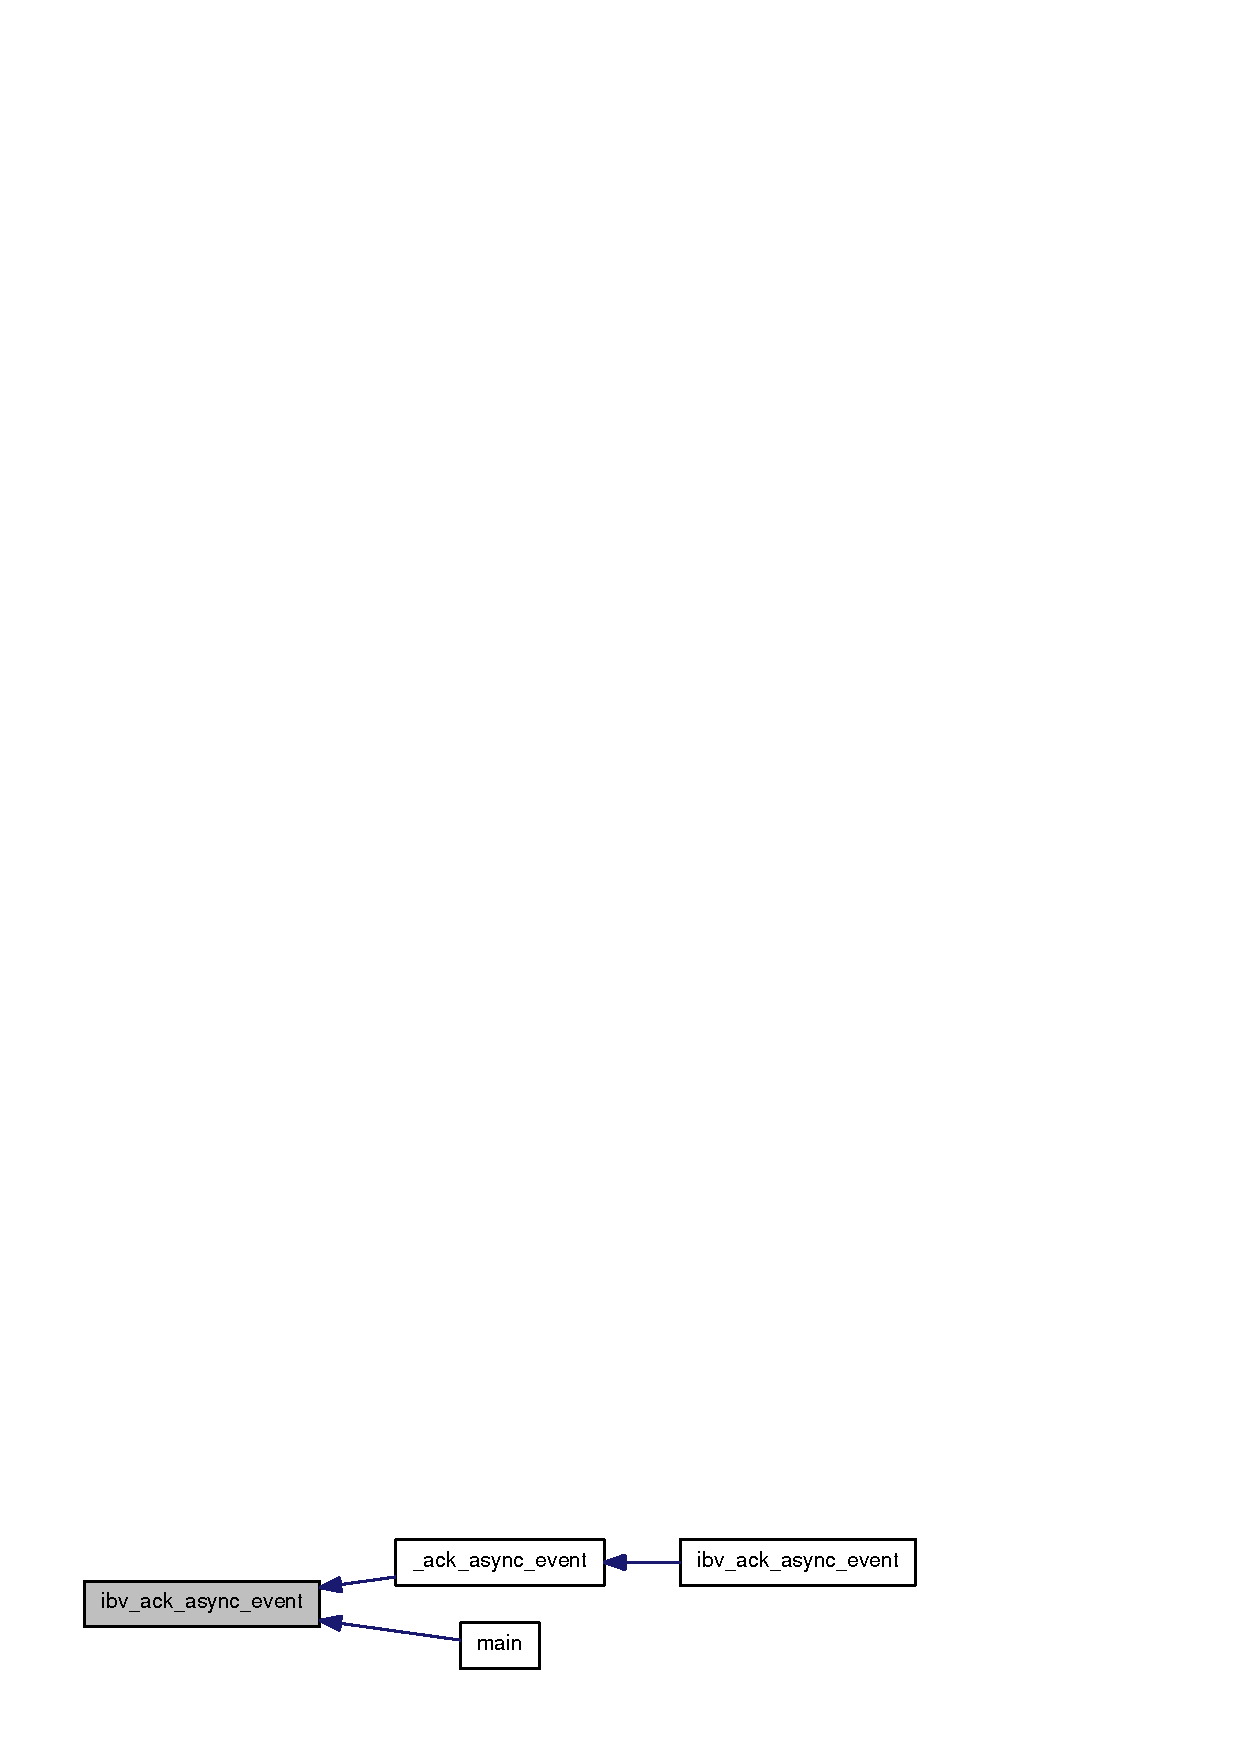
\includegraphics[width=222pt]{ibwrappers_8cpp_ac29b4d0a091a4e934d2c88aa3eb53fa3_icgraph}
\end{center}
\end{figure}
\hypertarget{ibwrappers_8cpp_a129903db6113f9cf09f2a8fb94275aa4}{
\index{ibwrappers.cpp@{ibwrappers.cpp}!ibv\_\-ack\_\-cq\_\-events@{ibv\_\-ack\_\-cq\_\-events}}
\index{ibv\_\-ack\_\-cq\_\-events@{ibv\_\-ack\_\-cq\_\-events}!ibwrappers.cpp@{ibwrappers.cpp}}
\subsubsection[{ibv\_\-ack\_\-cq\_\-events}]{\setlength{\rightskip}{0pt plus 5cm}void ibv\_\-ack\_\-cq\_\-events (struct ibv\_\-cq $\ast$ {\em cq}, \/  unsigned int {\em nevents})}}
\label{ibwrappers_8cpp_a129903db6113f9cf09f2a8fb94275aa4}


呼出しグラフ:\nopagebreak
\begin{figure}[H]
\begin{center}
\leavevmode
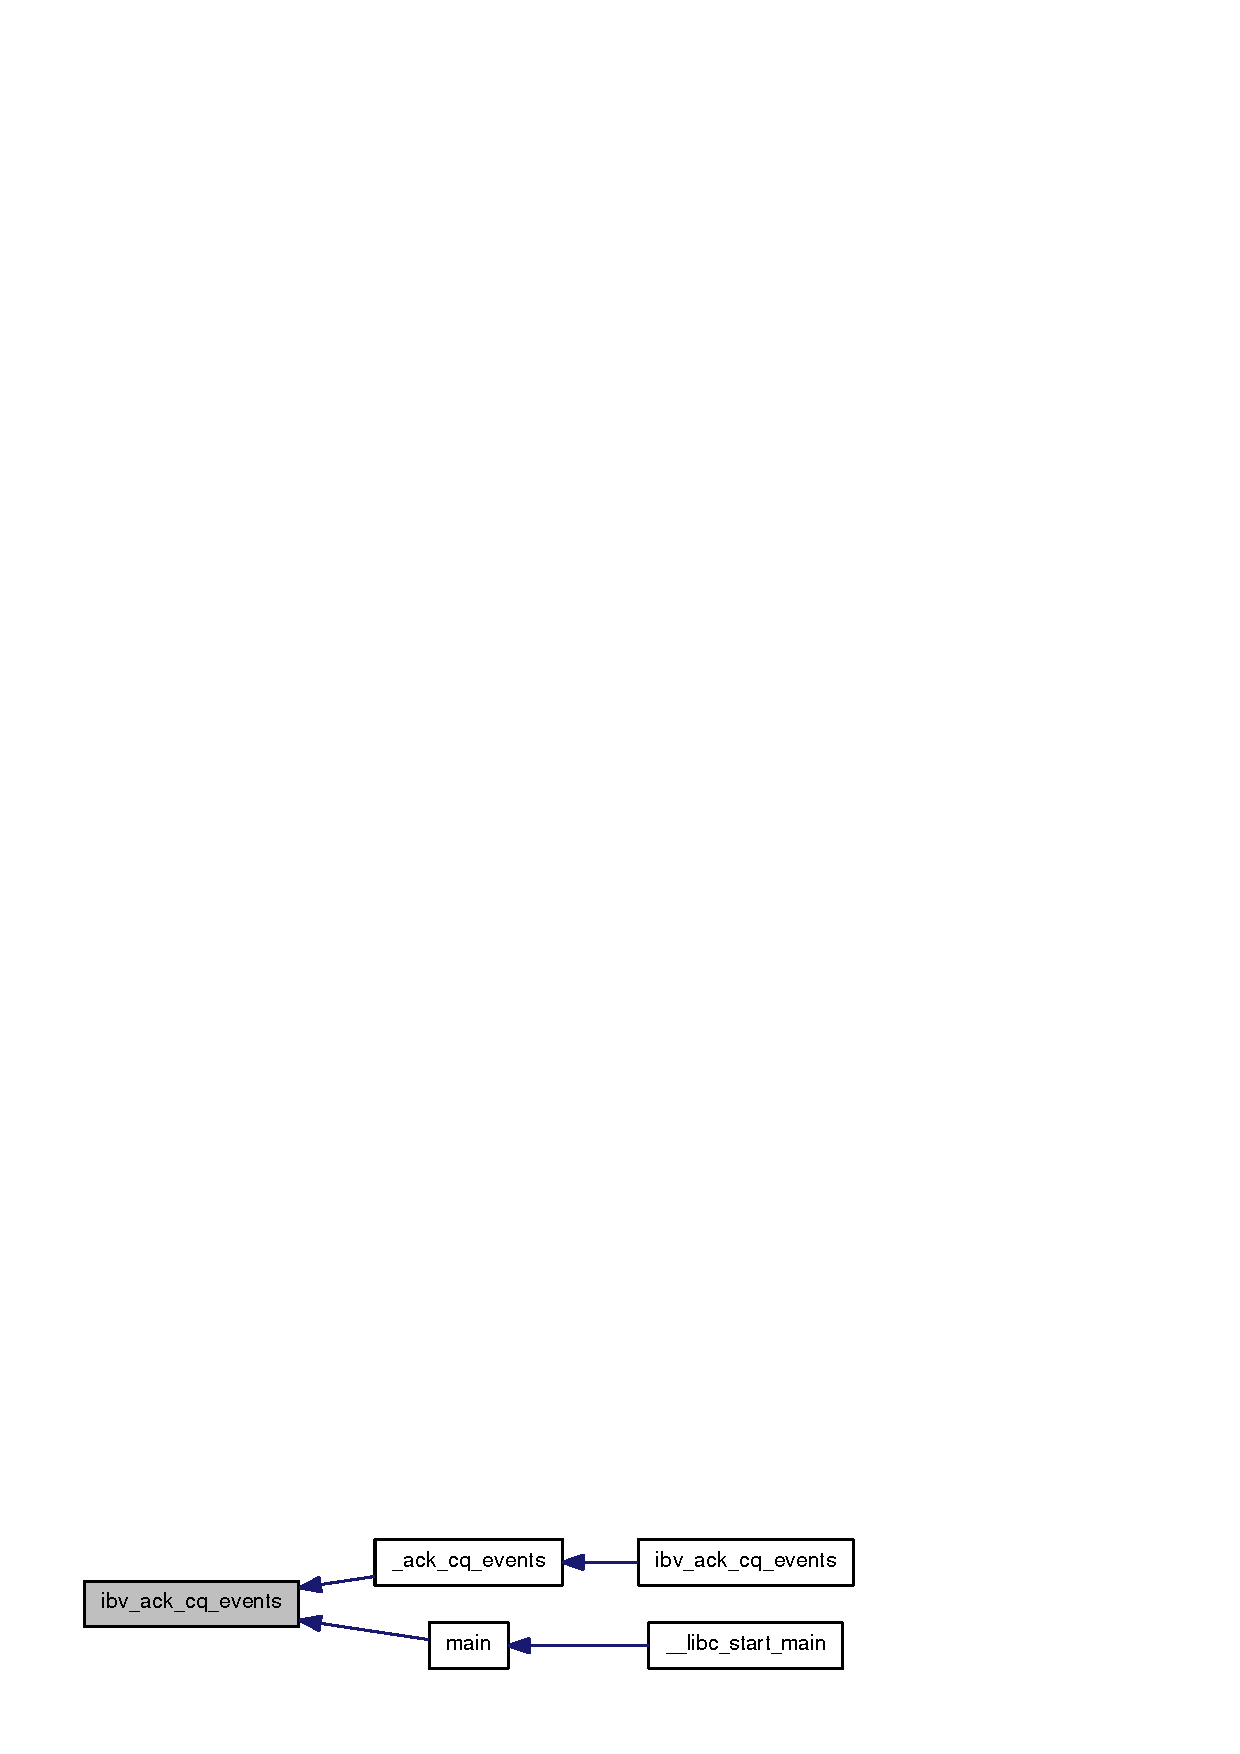
\includegraphics[width=207pt]{ibwrappers_8cpp_a129903db6113f9cf09f2a8fb94275aa4_icgraph}
\end{center}
\end{figure}
\hypertarget{ibwrappers_8cpp_a4d733171c73a340e292b66a91bd81401}{
\index{ibwrappers.cpp@{ibwrappers.cpp}!ibv\_\-create\_\-qp@{ibv\_\-create\_\-qp}}
\index{ibv\_\-create\_\-qp@{ibv\_\-create\_\-qp}!ibwrappers.cpp@{ibwrappers.cpp}}
\subsubsection[{ibv\_\-create\_\-qp}]{\setlength{\rightskip}{0pt plus 5cm}struct ibv\_\-qp$\ast$ ibv\_\-create\_\-qp (struct ibv\_\-pd $\ast$ {\em pd}, \/  struct ibv\_\-qp\_\-init\_\-attr $\ast$ {\em qp\_\-init\_\-attr})\hspace{0.3cm}{\ttfamily  \mbox{[}read\mbox{]}}}}
\label{ibwrappers_8cpp_a4d733171c73a340e292b66a91bd81401}


関数の呼び出しグラフ:\nopagebreak
\begin{figure}[H]
\begin{center}
\leavevmode
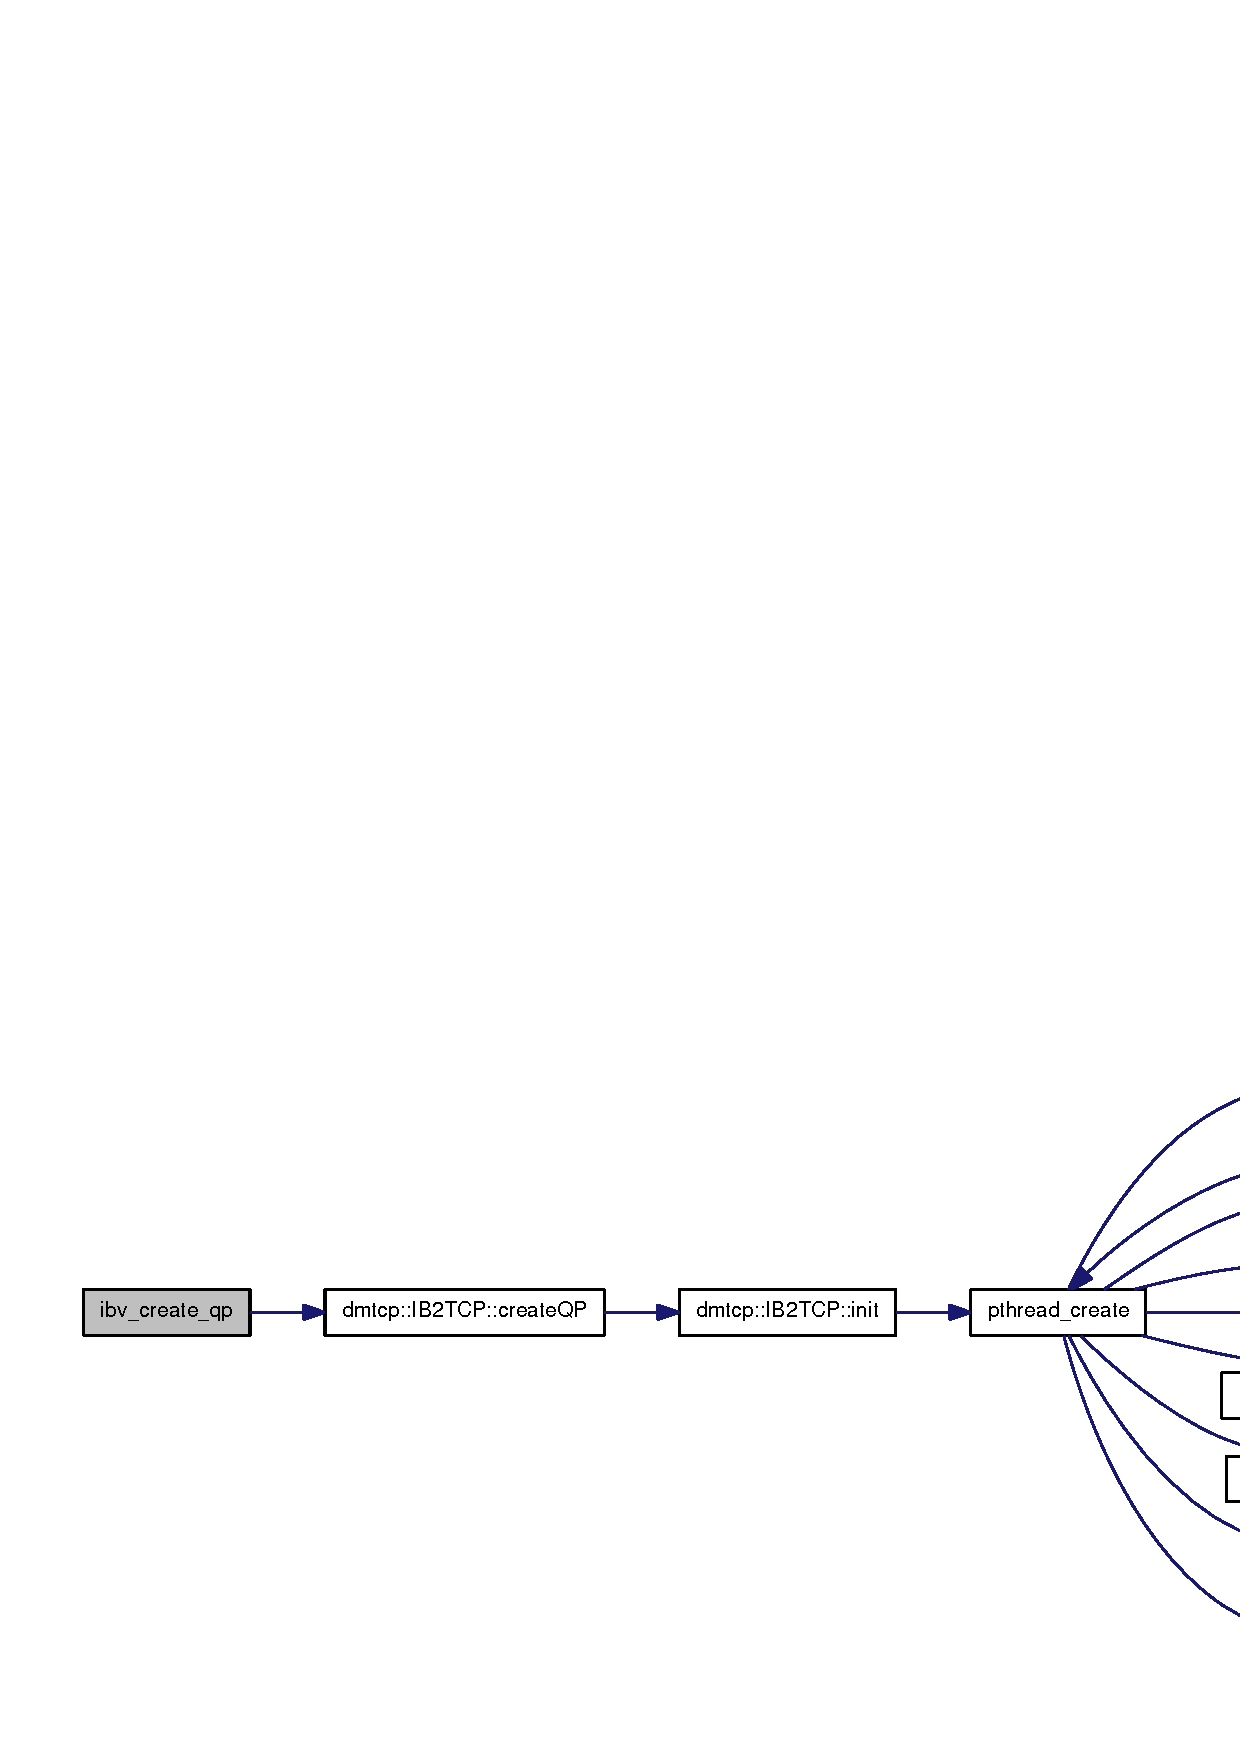
\includegraphics[width=420pt]{ibwrappers_8cpp_a4d733171c73a340e292b66a91bd81401_cgraph}
\end{center}
\end{figure}


呼出しグラフ:\nopagebreak
\begin{figure}[H]
\begin{center}
\leavevmode
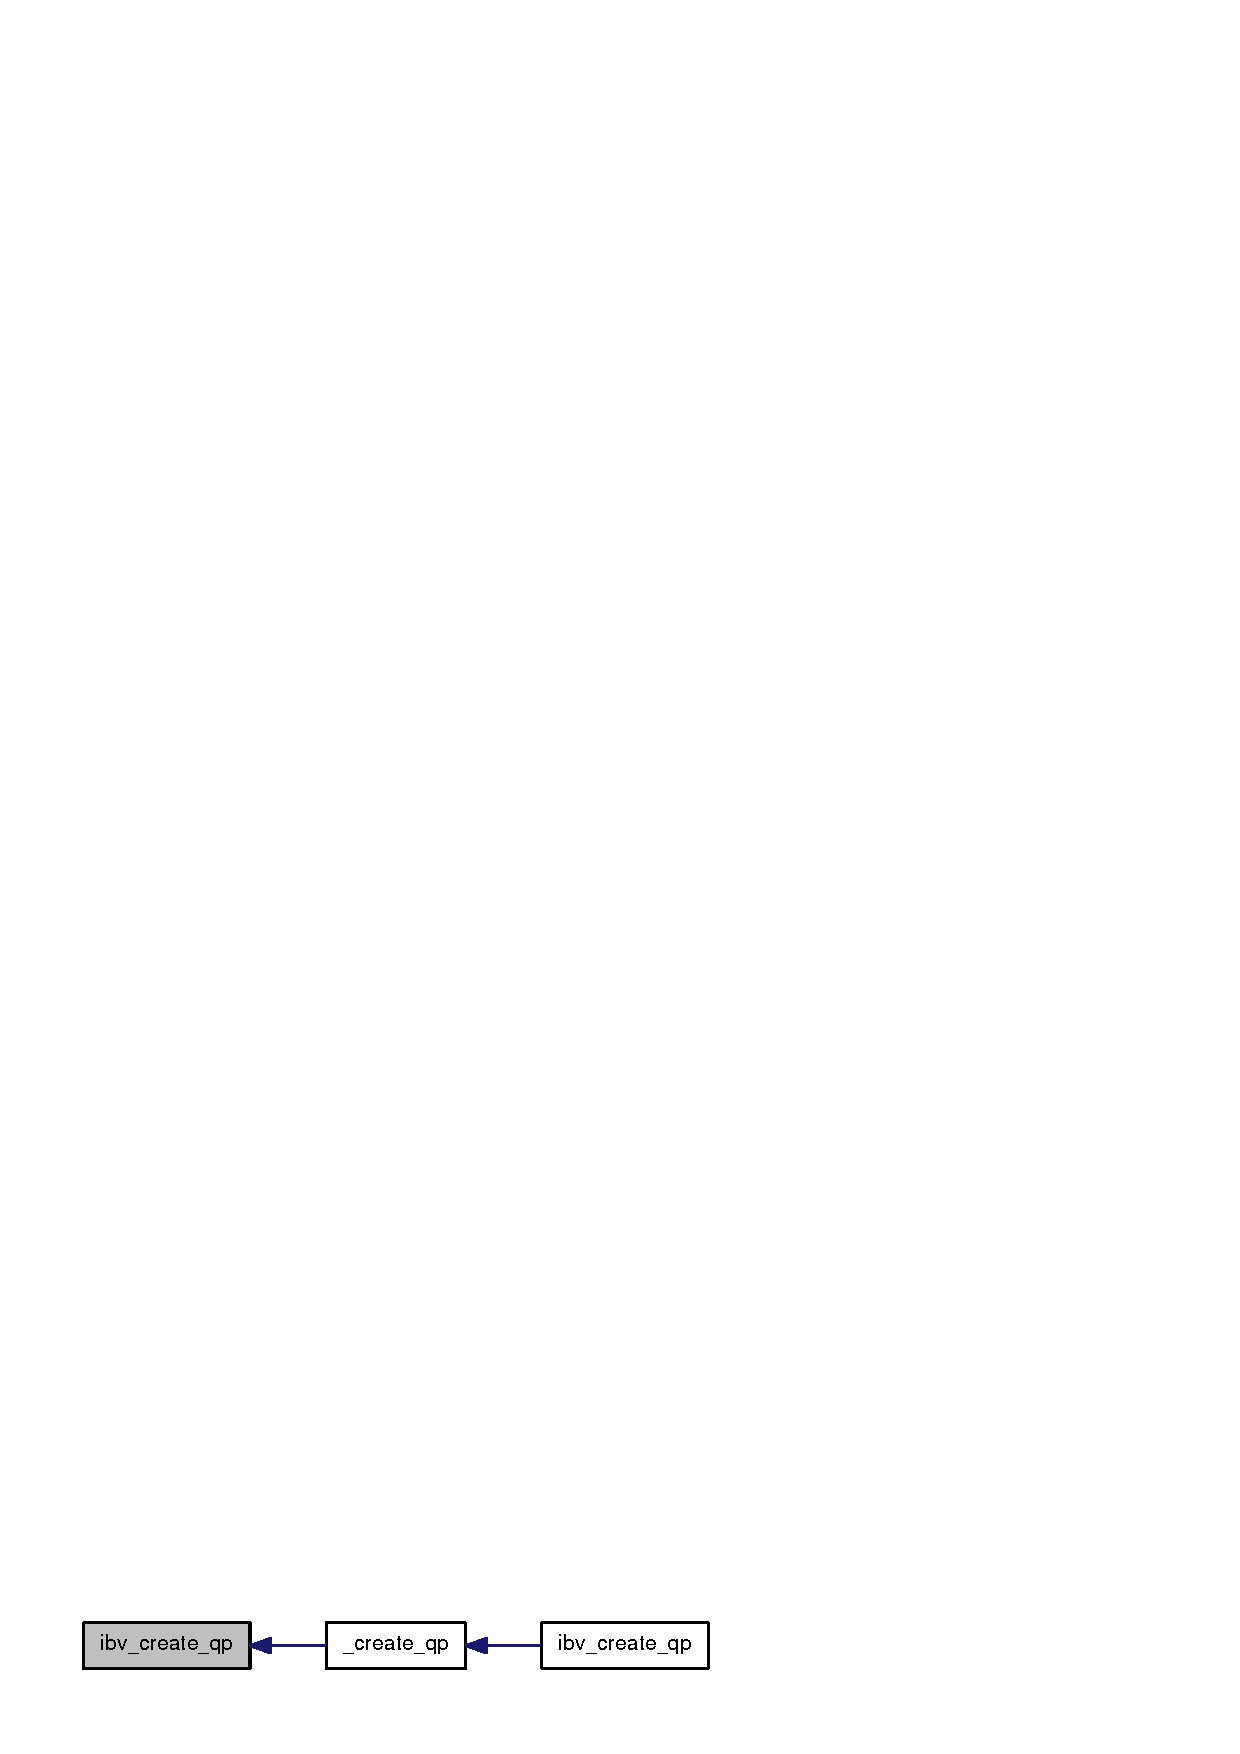
\includegraphics[width=172pt]{ibwrappers_8cpp_a4d733171c73a340e292b66a91bd81401_icgraph}
\end{center}
\end{figure}
\hypertarget{ibwrappers_8cpp_aa0fc78a4ee91da053d4d5be704223411}{
\index{ibwrappers.cpp@{ibwrappers.cpp}!ibv\_\-destroy\_\-qp@{ibv\_\-destroy\_\-qp}}
\index{ibv\_\-destroy\_\-qp@{ibv\_\-destroy\_\-qp}!ibwrappers.cpp@{ibwrappers.cpp}}
\subsubsection[{ibv\_\-destroy\_\-qp}]{\setlength{\rightskip}{0pt plus 5cm}int ibv\_\-destroy\_\-qp (struct ibv\_\-qp $\ast$ {\em qp})}}
\label{ibwrappers_8cpp_aa0fc78a4ee91da053d4d5be704223411}


呼出しグラフ:\nopagebreak
\begin{figure}[H]
\begin{center}
\leavevmode
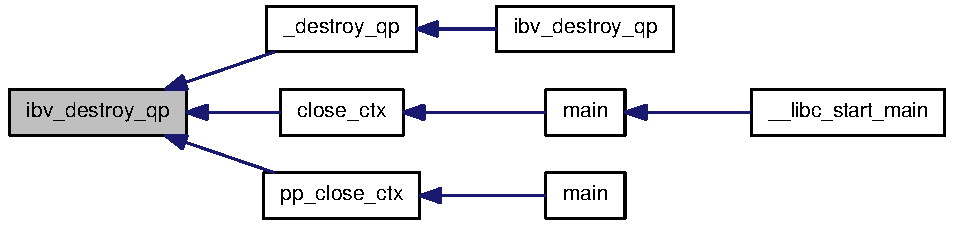
\includegraphics[width=247pt]{ibwrappers_8cpp_aa0fc78a4ee91da053d4d5be704223411_icgraph}
\end{center}
\end{figure}
\hypertarget{ibwrappers_8cpp_ab5c7015df6e9a99d1277f25b4cbb2418}{
\index{ibwrappers.cpp@{ibwrappers.cpp}!ibv\_\-get\_\-async\_\-event@{ibv\_\-get\_\-async\_\-event}}
\index{ibv\_\-get\_\-async\_\-event@{ibv\_\-get\_\-async\_\-event}!ibwrappers.cpp@{ibwrappers.cpp}}
\subsubsection[{ibv\_\-get\_\-async\_\-event}]{\setlength{\rightskip}{0pt plus 5cm}int ibv\_\-get\_\-async\_\-event (struct ibv\_\-context $\ast$ {\em context}, \/  struct ibv\_\-async\_\-event $\ast$ {\em event})}}
\label{ibwrappers_8cpp_ab5c7015df6e9a99d1277f25b4cbb2418}


呼出しグラフ:\nopagebreak
\begin{figure}[H]
\begin{center}
\leavevmode
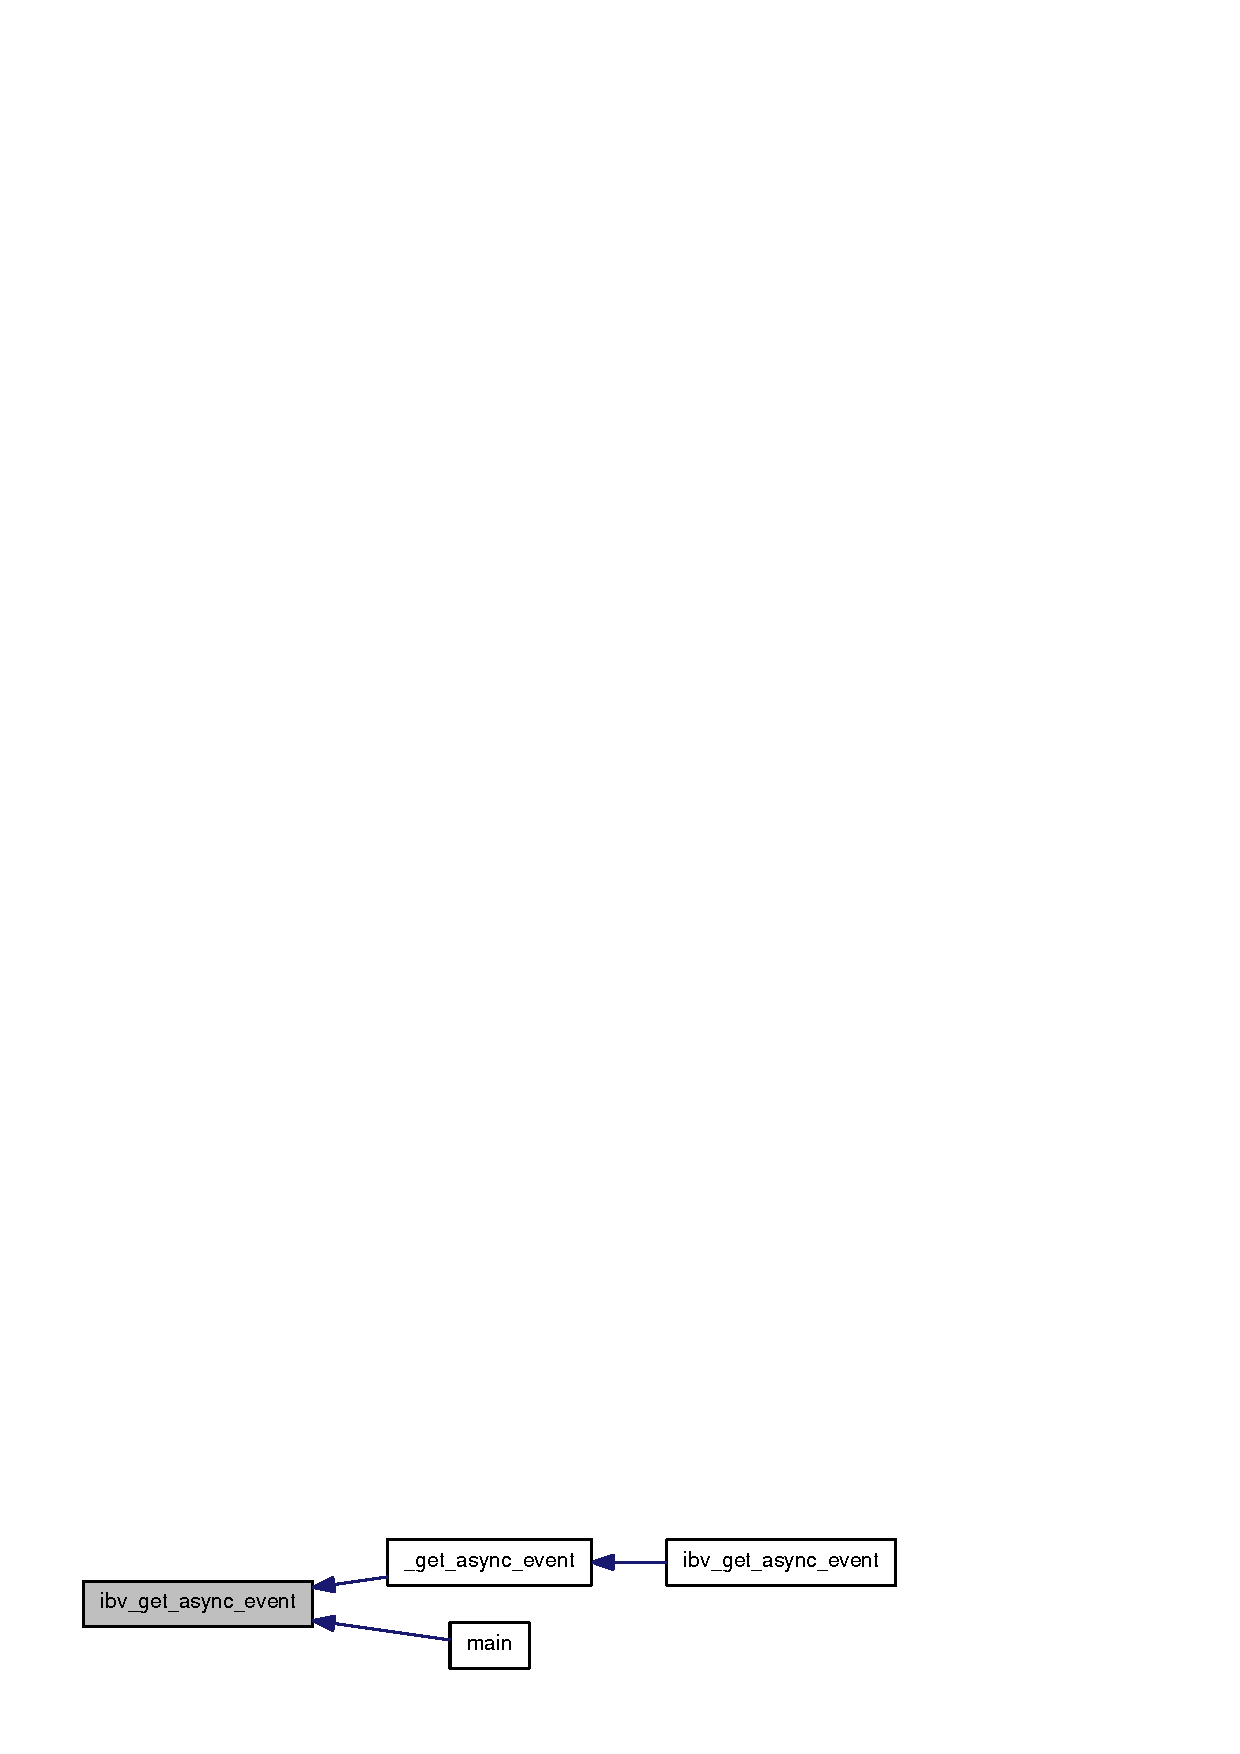
\includegraphics[width=217pt]{ibwrappers_8cpp_ab5c7015df6e9a99d1277f25b4cbb2418_icgraph}
\end{center}
\end{figure}
\hypertarget{ibwrappers_8cpp_a62c43f7b57bb22cce555cc2c853ac8bc}{
\index{ibwrappers.cpp@{ibwrappers.cpp}!ibv\_\-get\_\-cq\_\-event@{ibv\_\-get\_\-cq\_\-event}}
\index{ibv\_\-get\_\-cq\_\-event@{ibv\_\-get\_\-cq\_\-event}!ibwrappers.cpp@{ibwrappers.cpp}}
\subsubsection[{ibv\_\-get\_\-cq\_\-event}]{\setlength{\rightskip}{0pt plus 5cm}int ibv\_\-get\_\-cq\_\-event (struct ibv\_\-comp\_\-channel $\ast$ {\em channel}, \/  struct ibv\_\-cq $\ast$$\ast$ {\em cq}, \/  void $\ast$$\ast$ {\em cq\_\-context})}}
\label{ibwrappers_8cpp_a62c43f7b57bb22cce555cc2c853ac8bc}


呼出しグラフ:\nopagebreak
\begin{figure}[H]
\begin{center}
\leavevmode
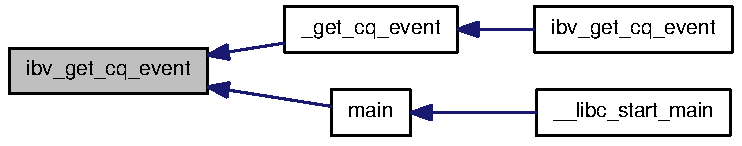
\includegraphics[width=196pt]{ibwrappers_8cpp_a62c43f7b57bb22cce555cc2c853ac8bc_icgraph}
\end{center}
\end{figure}
\hypertarget{ibwrappers_8cpp_a7775daa82f7e8814ead91b40dbd5eb95}{
\index{ibwrappers.cpp@{ibwrappers.cpp}!ibv\_\-modify\_\-qp@{ibv\_\-modify\_\-qp}}
\index{ibv\_\-modify\_\-qp@{ibv\_\-modify\_\-qp}!ibwrappers.cpp@{ibwrappers.cpp}}
\subsubsection[{ibv\_\-modify\_\-qp}]{\setlength{\rightskip}{0pt plus 5cm}int ibv\_\-modify\_\-qp (struct ibv\_\-qp $\ast$ {\em qp}, \/  struct ibv\_\-qp\_\-attr $\ast$ {\em attr}, \/  int {\em attr\_\-mask})}}
\label{ibwrappers_8cpp_a7775daa82f7e8814ead91b40dbd5eb95}


関数の呼び出しグラフ:\nopagebreak
\begin{figure}[H]
\begin{center}
\leavevmode
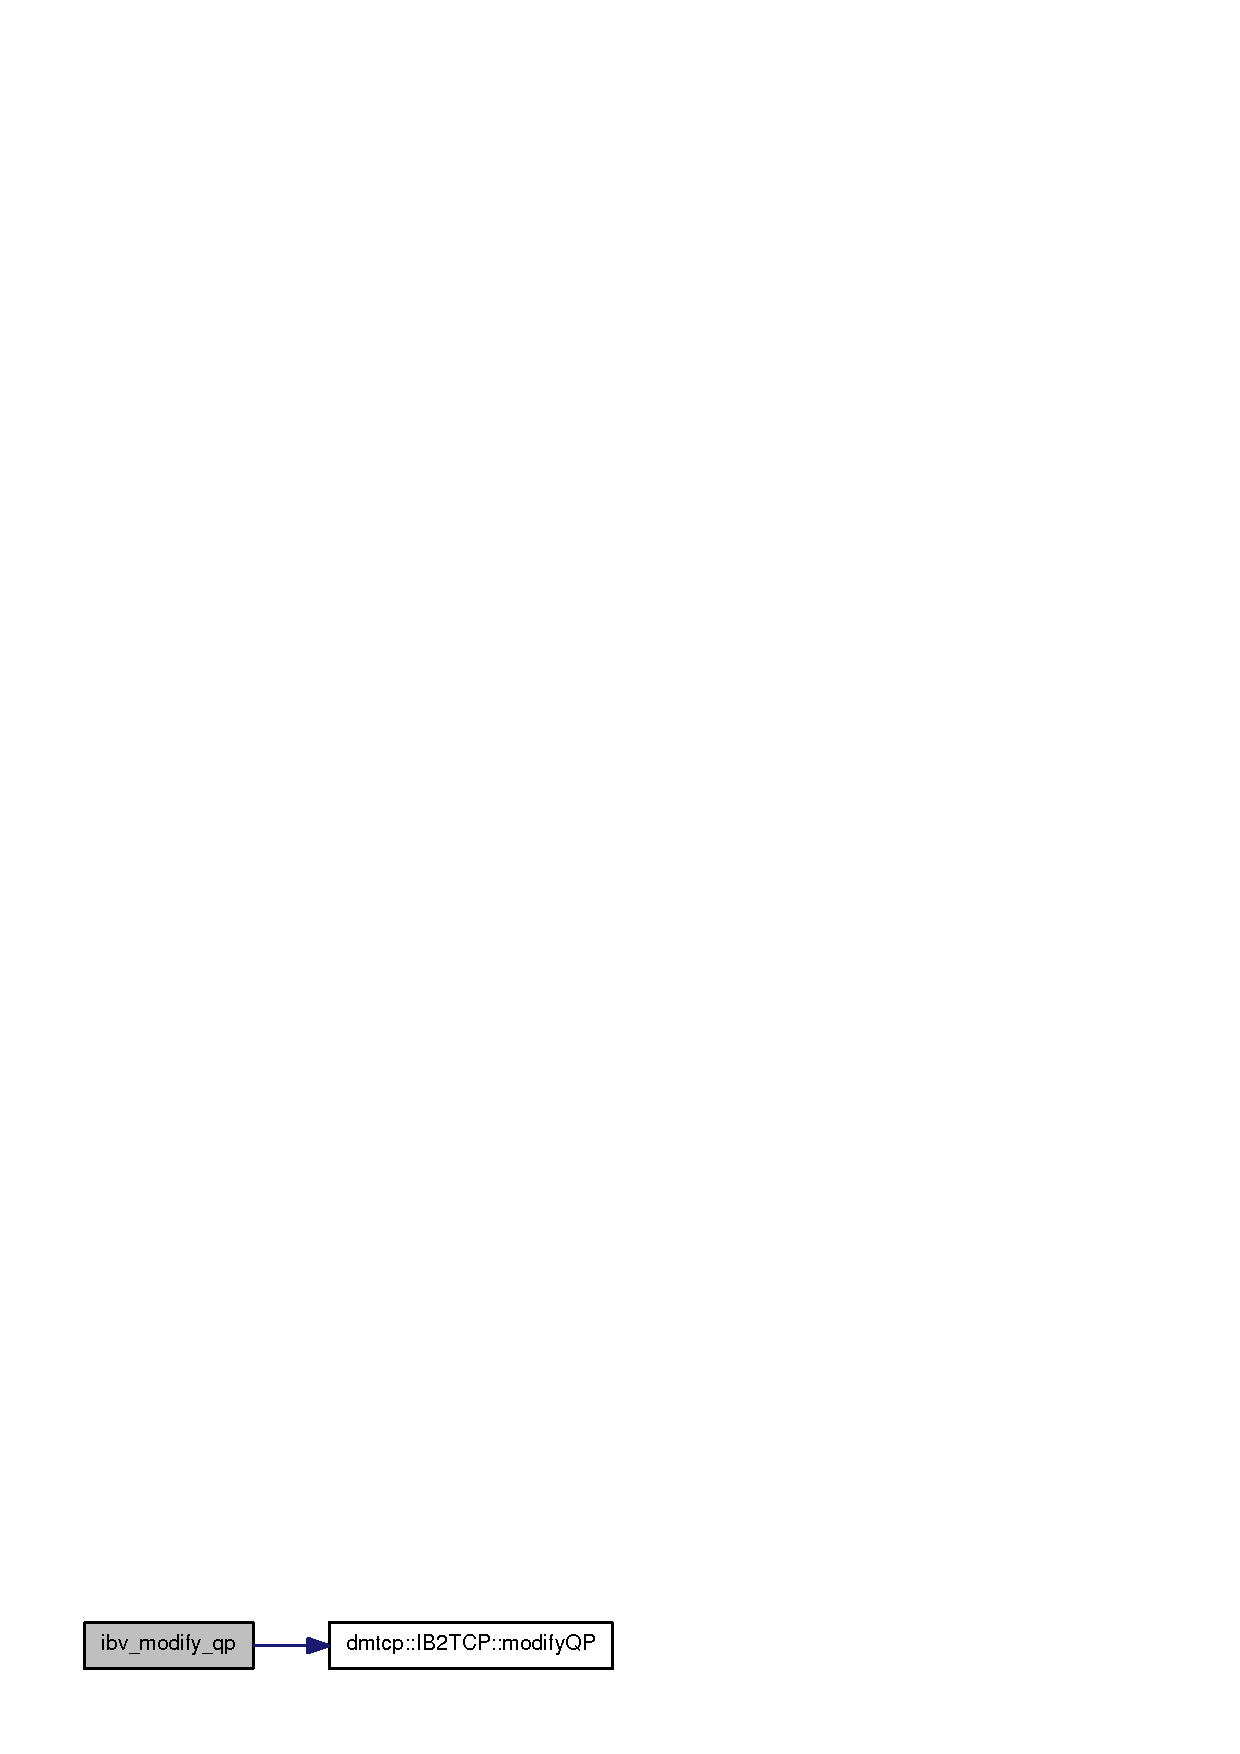
\includegraphics[width=149pt]{ibwrappers_8cpp_a7775daa82f7e8814ead91b40dbd5eb95_cgraph}
\end{center}
\end{figure}


呼出しグラフ:\nopagebreak
\begin{figure}[H]
\begin{center}
\leavevmode
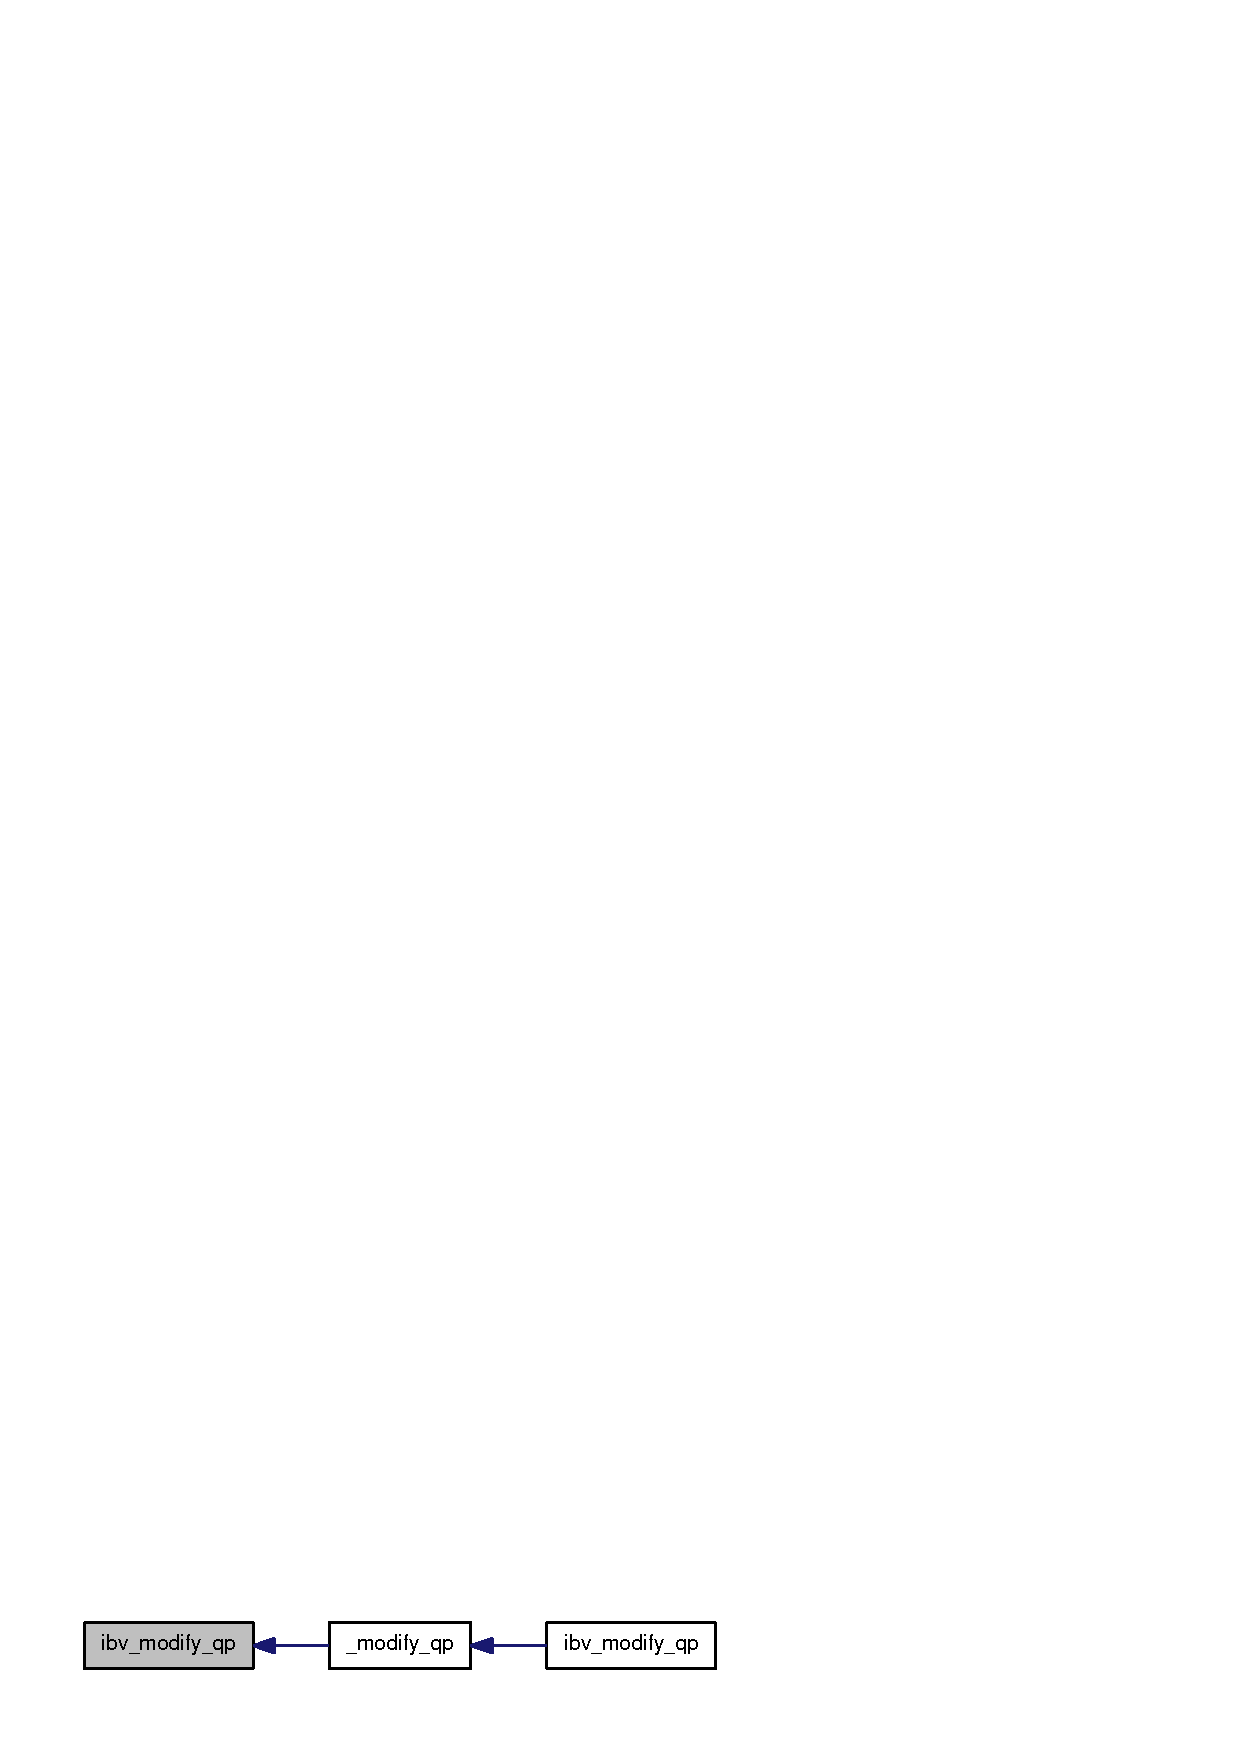
\includegraphics[width=174pt]{ibwrappers_8cpp_a7775daa82f7e8814ead91b40dbd5eb95_icgraph}
\end{center}
\end{figure}
\hypertarget{ibwrappers_8cpp_a8e14823e543fe663dd0bffe6e05708cd}{
\index{ibwrappers.cpp@{ibwrappers.cpp}!ibv\_\-open\_\-device@{ibv\_\-open\_\-device}}
\index{ibv\_\-open\_\-device@{ibv\_\-open\_\-device}!ibwrappers.cpp@{ibwrappers.cpp}}
\subsubsection[{ibv\_\-open\_\-device}]{\setlength{\rightskip}{0pt plus 5cm}struct ibv\_\-context$\ast$ ibv\_\-open\_\-device (struct ibv\_\-device $\ast$ {\em dev})\hspace{0.3cm}{\ttfamily  \mbox{[}read\mbox{]}}}}
\label{ibwrappers_8cpp_a8e14823e543fe663dd0bffe6e05708cd}


関数の呼び出しグラフ:\nopagebreak
\begin{figure}[H]
\begin{center}
\leavevmode
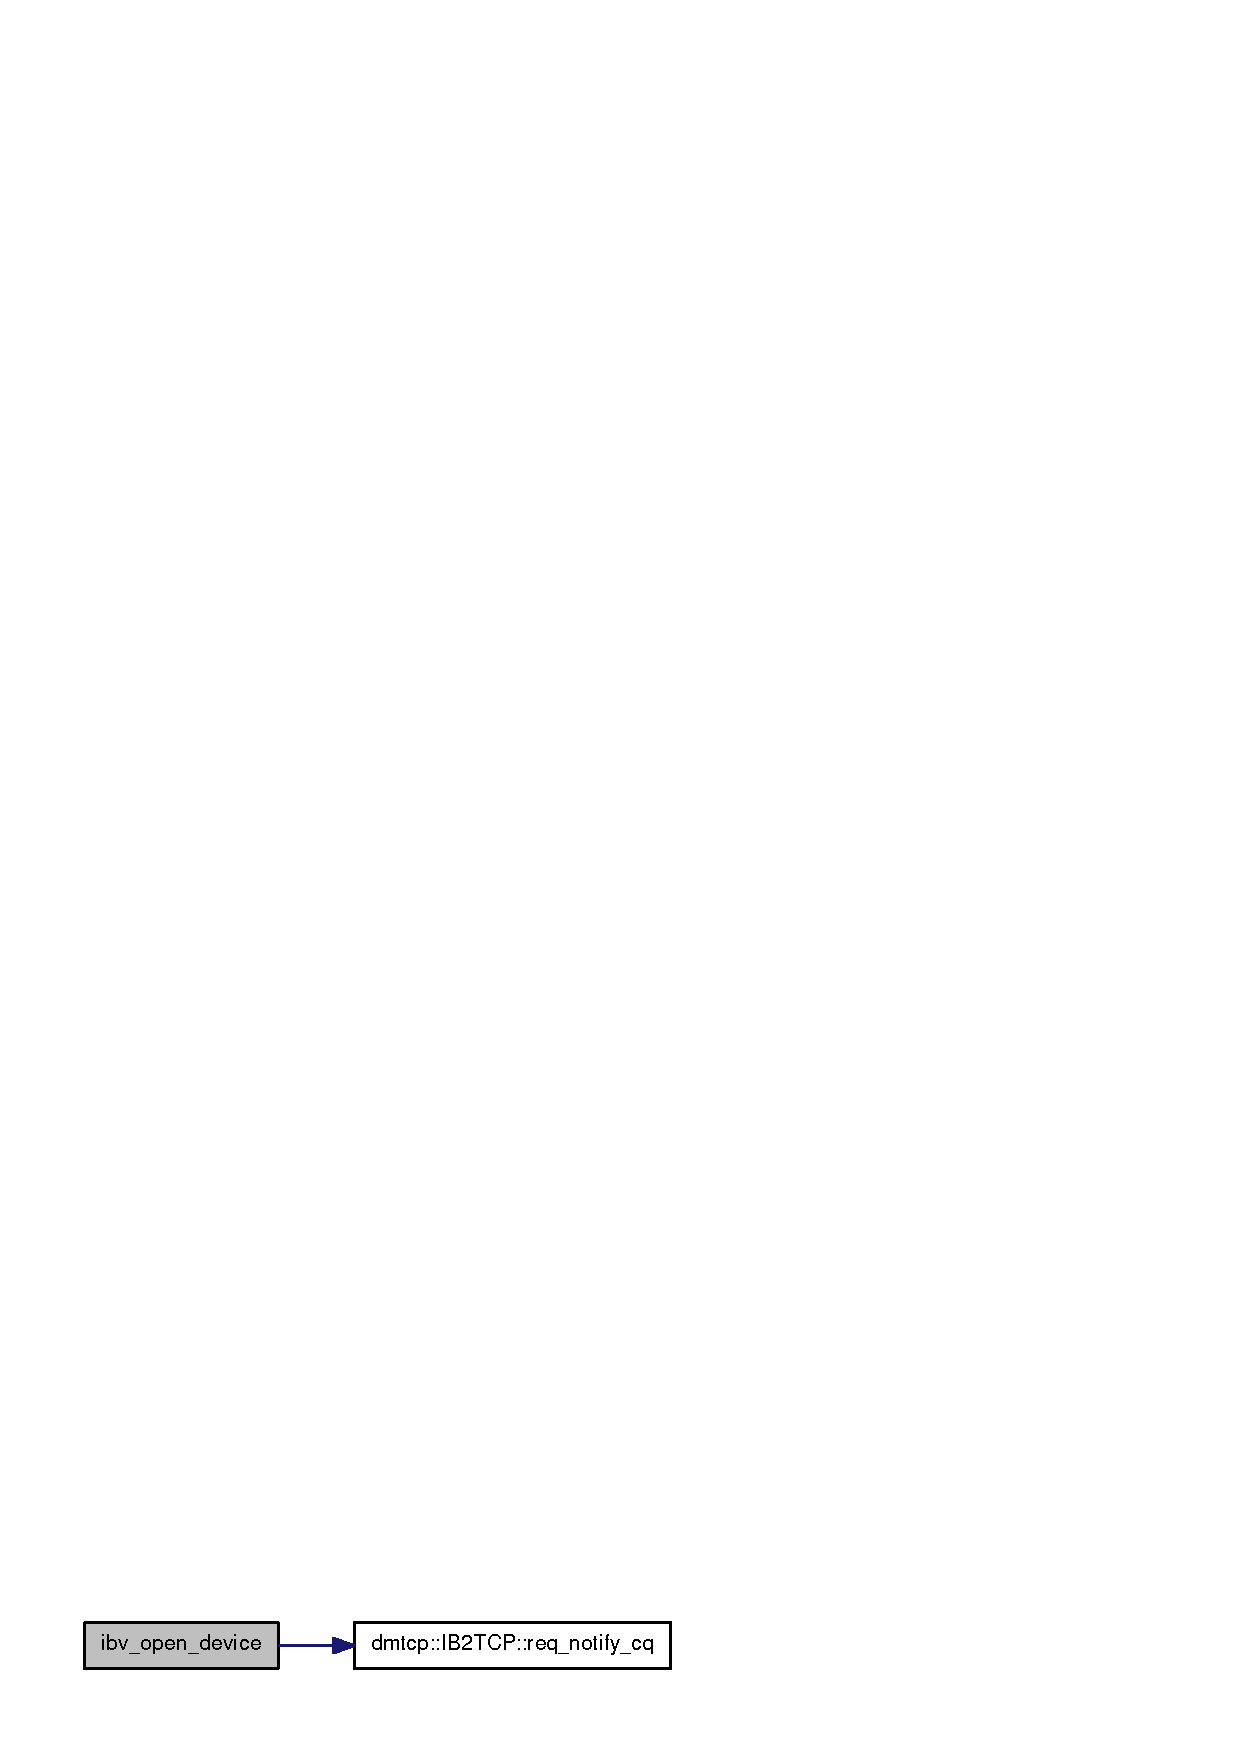
\includegraphics[width=163pt]{ibwrappers_8cpp_a8e14823e543fe663dd0bffe6e05708cd_cgraph}
\end{center}
\end{figure}


呼出しグラフ:\nopagebreak
\begin{figure}[H]
\begin{center}
\leavevmode
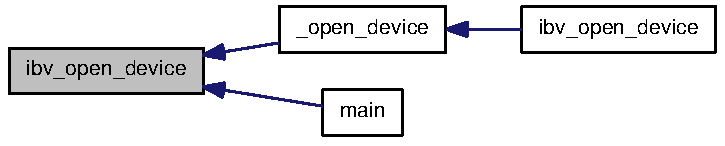
\includegraphics[width=192pt]{ibwrappers_8cpp_a8e14823e543fe663dd0bffe6e05708cd_icgraph}
\end{center}
\end{figure}


\subsection{変数}
\hypertarget{ibwrappers_8cpp_a4eb6e16937eb7b9a7a35540e7a49710d}{
\index{ibwrappers.cpp@{ibwrappers.cpp}!isVirtIB@{isVirtIB}}
\index{isVirtIB@{isVirtIB}!ibwrappers.cpp@{ibwrappers.cpp}}
\subsubsection[{isVirtIB}]{\setlength{\rightskip}{0pt plus 5cm}int {\bf isVirtIB}}}
\label{ibwrappers_8cpp_a4eb6e16937eb7b9a7a35540e7a49710d}

\hypertarget{ibwrappers_8h}{
\section{contrib/ib2tcp/ibwrappers.h}
\label{ibwrappers_8h}\index{contrib/ib2tcp/ibwrappers.h@{contrib/ib2tcp/ibwrappers.h}}
}
{\ttfamily \#include \char`\"{}dmtcp.h\char`\"{}}\par
ibwrappers.hのインクルード依存関係図\nopagebreak
\begin{figure}[H]
\begin{center}
\leavevmode
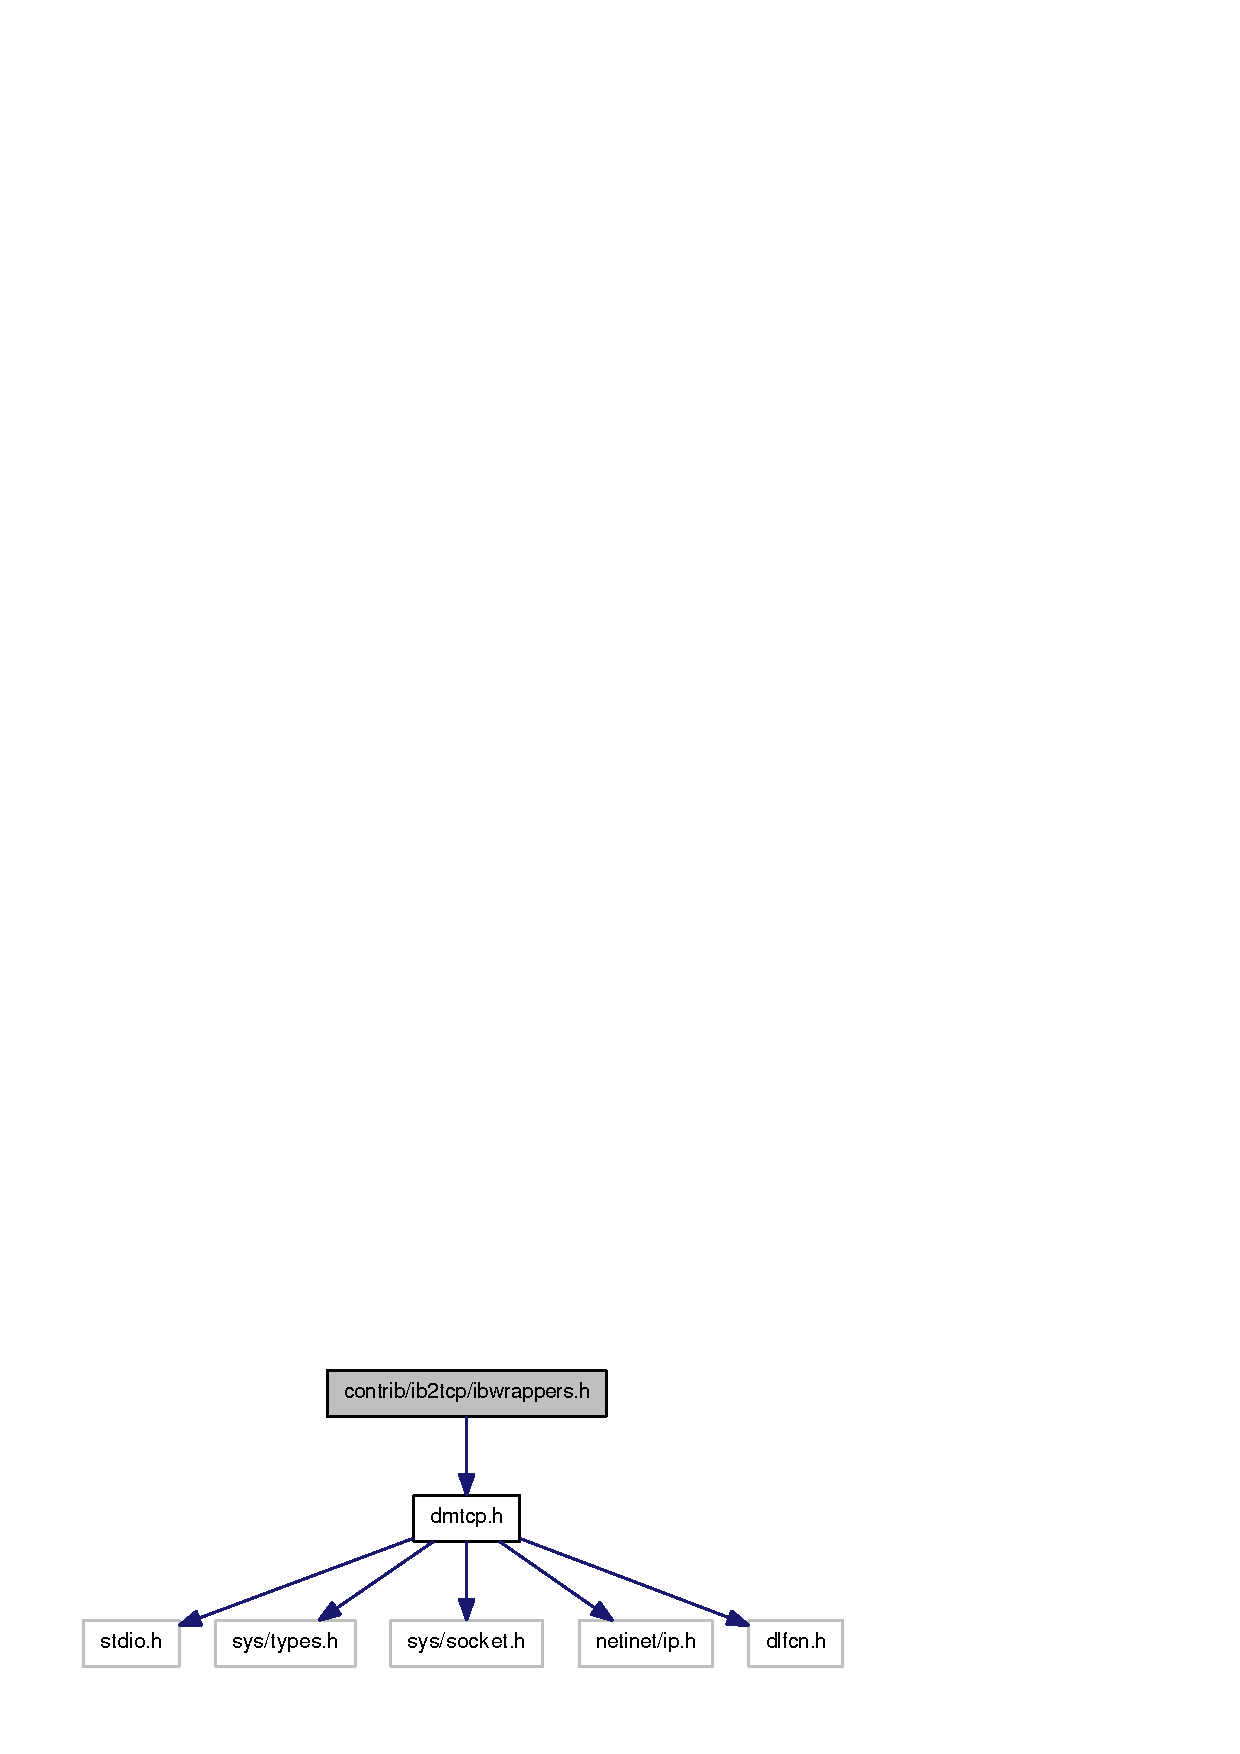
\includegraphics[width=204pt]{ibwrappers_8h__incl}
\end{center}
\end{figure}
このグラフは、どのファイルから直接、間接的にインクルードされているかを示しています。\nopagebreak
\begin{figure}[H]
\begin{center}
\leavevmode
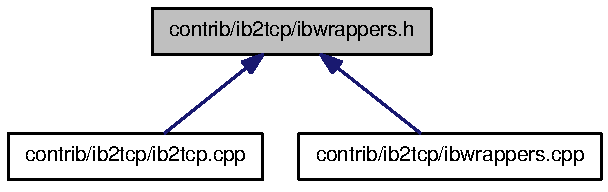
\includegraphics[width=164pt]{ibwrappers_8h__dep__incl}
\end{center}
\end{figure}
\subsection*{マクロ定義}
\begin{DoxyCompactItemize}
\item 
\#define \hyperlink{ibwrappers_8h_a5722a172eb77881f16b3261936b9631d}{\_\-real\_\-ibv\_\-get\_\-device\_\-list}~NEXT\_\-FNC(ibv\_\-get\_\-device\_\-list)
\item 
\#define \hyperlink{ibwrappers_8h_ace0616b8e04985dbc959175c4011fd01}{\_\-real\_\-ibv\_\-open\_\-device}~NEXT\_\-FNC(ibv\_\-open\_\-device)
\item 
\#define \hyperlink{ibwrappers_8h_a4d1a1a86d8377f830b91fd7e66c8856f}{\_\-real\_\-ibv\_\-get\_\-device\_\-name}~NEXT\_\-FNC(ibv\_\-get\_\-device\_\-name)
\item 
\#define \hyperlink{ibwrappers_8h_aed526ddcb01cd61aaf5dd163de335431}{\_\-real\_\-ibv\_\-query\_\-device}~NEXT\_\-FNC(ibv\_\-query\_\-device)
\item 
\#define \hyperlink{ibwrappers_8h_ad518fc956b5401ae5410d844545e58e3}{\_\-real\_\-ibv\_\-query\_\-port}~NEXT\_\-FNC(ibv\_\-query\_\-port)
\item 
\#define \hyperlink{ibwrappers_8h_a12342f2d362fd9dc398062f256c44305}{\_\-real\_\-ibv\_\-query\_\-pkey}~NEXT\_\-FNC(ibv\_\-query\_\-pkey)
\item 
\#define \hyperlink{ibwrappers_8h_aa62d2f84d4aceaaa51c52964d3601aa7}{\_\-real\_\-ibv\_\-query\_\-gid}~NEXT\_\-FNC(ibv\_\-query\_\-gid)
\item 
\#define \hyperlink{ibwrappers_8h_ab1b287cab0f67737416eaebaaae61573}{\_\-real\_\-ibv\_\-get\_\-cq\_\-event}~NEXT\_\-FNC(ibv\_\-get\_\-cq\_\-event)
\item 
\#define \hyperlink{ibwrappers_8h_a151ab74b6cab8e0797c29cdec8d2c1a3}{\_\-real\_\-ibv\_\-get\_\-async\_\-event}~NEXT\_\-FNC(ibv\_\-get\_\-async\_\-event)
\item 
\#define \hyperlink{ibwrappers_8h_a032a75dfad915ee40de344739047f3dd}{\_\-real\_\-ibv\_\-ack\_\-async\_\-event}~NEXT\_\-FNC(ibv\_\-ack\_\-async\_\-event)
\item 
\#define \hyperlink{ibwrappers_8h_a0064314f71e9c26c0a91a0afb39e34b4}{\_\-real\_\-ibv\_\-get\_\-device\_\-guid}~NEXT\_\-FNC(ibv\_\-get\_\-device\_\-guid)
\item 
\#define \hyperlink{ibwrappers_8h_ab7f4fde2b7665b9f1d37b96ed947d223}{\_\-real\_\-ibv\_\-create\_\-comp\_\-channel}~NEXT\_\-FNC(ibv\_\-create\_\-comp\_\-channel)
\item 
\#define \hyperlink{ibwrappers_8h_a11d935d64bfb3be5e54d68c0b20db145}{\_\-real\_\-ibv\_\-destroy\_\-comp\_\-channel}~NEXT\_\-FNC(ibv\_\-destroy\_\-comp\_\-channel)
\item 
\#define \hyperlink{ibwrappers_8h_ab775bd2498244220f6726cd33bb477cf}{\_\-real\_\-ibv\_\-resize\_\-cq}~NEXT\_\-FNC(ibv\_\-resize\_\-cq)
\item 
\#define \hyperlink{ibwrappers_8h_a6084ae1a71546440c1ef416c7a1c07f9}{\_\-real\_\-ibv\_\-alloc\_\-pd}~NEXT\_\-FNC(ibv\_\-alloc\_\-pd)
\item 
\#define \hyperlink{ibwrappers_8h_a39d902077a9cd27f45e9fefb8f3f2d57}{\_\-real\_\-ibv\_\-reg\_\-mr}~NEXT\_\-FNC(ibv\_\-reg\_\-mr)
\item 
\#define \hyperlink{ibwrappers_8h_a3d6171b241dcfce2c595a250ffc7f37b}{\_\-real\_\-ibv\_\-create\_\-cq}~NEXT\_\-FNC(ibv\_\-create\_\-cq)
\item 
\#define \hyperlink{ibwrappers_8h_ae7354de97c76d149bec43642f9f237c9}{\_\-real\_\-ibv\_\-create\_\-srq}~NEXT\_\-FNC(ibv\_\-create\_\-srq)
\item 
\#define \hyperlink{ibwrappers_8h_a87f96f572e23c216b2810fb4582e5494}{\_\-real\_\-ibv\_\-modify\_\-srq}~NEXT\_\-FNC(ibv\_\-modify\_\-srq)
\item 
\#define \hyperlink{ibwrappers_8h_a29a8bace1fd953a0770fb8d5f1bc5e3e}{\_\-real\_\-ibv\_\-query\_\-srq}~NEXT\_\-FNC(ibv\_\-query\_\-srq)
\item 
\#define \hyperlink{ibwrappers_8h_a803881f8bc8b25729328186164f8bc26}{\_\-real\_\-ibv\_\-create\_\-qp}~NEXT\_\-FNC(ibv\_\-create\_\-qp)
\item 
\#define \hyperlink{ibwrappers_8h_a2330eddde5bde51b1feeea4af28bb8d8}{\_\-real\_\-ibv\_\-modify\_\-qp}~NEXT\_\-FNC(ibv\_\-modify\_\-qp)
\item 
\#define \hyperlink{ibwrappers_8h_ace5b18884c17f8937f090a940470da19}{\_\-real\_\-ibv\_\-query\_\-qp}~NEXT\_\-FNC(ibv\_\-query\_\-qp)
\item 
\#define \hyperlink{ibwrappers_8h_a010602debd87e10ca375517282848926}{\_\-real\_\-ibv\_\-ack\_\-cq\_\-events}~NEXT\_\-FNC(ibv\_\-ack\_\-cq\_\-events)
\item 
\#define \hyperlink{ibwrappers_8h_ad0074809ec543cf01738a2c3b3c79268}{\_\-real\_\-ibv\_\-destroy\_\-cq}~NEXT\_\-FNC(ibv\_\-destroy\_\-cq)
\item 
\#define \hyperlink{ibwrappers_8h_a06c22141e2ffda9f3bdaf431b6c4a9a2}{\_\-real\_\-ibv\_\-destroy\_\-qp}~NEXT\_\-FNC(ibv\_\-destroy\_\-qp)
\item 
\#define \hyperlink{ibwrappers_8h_ad88f3cee94e010c6c41f125c4067aff3}{\_\-real\_\-ibv\_\-destroy\_\-srq}~NEXT\_\-FNC(ibv\_\-destroy\_\-srq)
\item 
\#define \hyperlink{ibwrappers_8h_a2abc9e51e66dd18e9530e769794d66eb}{\_\-real\_\-ibv\_\-dereg\_\-mr}~NEXT\_\-FNC(ibv\_\-dereg\_\-mr)
\item 
\#define \hyperlink{ibwrappers_8h_a1fbf0e47bdc746a2806206791498a22f}{\_\-real\_\-ibv\_\-dealloc\_\-pd}~NEXT\_\-FNC(ibv\_\-dealloc\_\-pd)
\item 
\#define \hyperlink{ibwrappers_8h_ae0b826157f6fbfad2a83073a9e5421a0}{\_\-real\_\-ibv\_\-close\_\-device}~NEXT\_\-FNC(ibv\_\-close\_\-device)
\item 
\#define \hyperlink{ibwrappers_8h_a6555d664658212cce236ae7bae590ce9}{\_\-real\_\-ibv\_\-free\_\-device\_\-list}~NEXT\_\-FNC(ibv\_\-free\_\-device\_\-list)
\end{DoxyCompactItemize}


\subsection{マクロ定義}
\hypertarget{ibwrappers_8h_a032a75dfad915ee40de344739047f3dd}{
\index{ibwrappers.h@{ibwrappers.h}!\_\-real\_\-ibv\_\-ack\_\-async\_\-event@{\_\-real\_\-ibv\_\-ack\_\-async\_\-event}}
\index{\_\-real\_\-ibv\_\-ack\_\-async\_\-event@{\_\-real\_\-ibv\_\-ack\_\-async\_\-event}!ibwrappers.h@{ibwrappers.h}}
\subsubsection[{\_\-real\_\-ibv\_\-ack\_\-async\_\-event}]{\setlength{\rightskip}{0pt plus 5cm}\#define \_\-real\_\-ibv\_\-ack\_\-async\_\-event~NEXT\_\-FNC(ibv\_\-ack\_\-async\_\-event)}}
\label{ibwrappers_8h_a032a75dfad915ee40de344739047f3dd}
\hypertarget{ibwrappers_8h_a010602debd87e10ca375517282848926}{
\index{ibwrappers.h@{ibwrappers.h}!\_\-real\_\-ibv\_\-ack\_\-cq\_\-events@{\_\-real\_\-ibv\_\-ack\_\-cq\_\-events}}
\index{\_\-real\_\-ibv\_\-ack\_\-cq\_\-events@{\_\-real\_\-ibv\_\-ack\_\-cq\_\-events}!ibwrappers.h@{ibwrappers.h}}
\subsubsection[{\_\-real\_\-ibv\_\-ack\_\-cq\_\-events}]{\setlength{\rightskip}{0pt plus 5cm}\#define \_\-real\_\-ibv\_\-ack\_\-cq\_\-events~NEXT\_\-FNC(ibv\_\-ack\_\-cq\_\-events)}}
\label{ibwrappers_8h_a010602debd87e10ca375517282848926}
\hypertarget{ibwrappers_8h_a6084ae1a71546440c1ef416c7a1c07f9}{
\index{ibwrappers.h@{ibwrappers.h}!\_\-real\_\-ibv\_\-alloc\_\-pd@{\_\-real\_\-ibv\_\-alloc\_\-pd}}
\index{\_\-real\_\-ibv\_\-alloc\_\-pd@{\_\-real\_\-ibv\_\-alloc\_\-pd}!ibwrappers.h@{ibwrappers.h}}
\subsubsection[{\_\-real\_\-ibv\_\-alloc\_\-pd}]{\setlength{\rightskip}{0pt plus 5cm}\#define \_\-real\_\-ibv\_\-alloc\_\-pd~NEXT\_\-FNC(ibv\_\-alloc\_\-pd)}}
\label{ibwrappers_8h_a6084ae1a71546440c1ef416c7a1c07f9}
\hypertarget{ibwrappers_8h_ae0b826157f6fbfad2a83073a9e5421a0}{
\index{ibwrappers.h@{ibwrappers.h}!\_\-real\_\-ibv\_\-close\_\-device@{\_\-real\_\-ibv\_\-close\_\-device}}
\index{\_\-real\_\-ibv\_\-close\_\-device@{\_\-real\_\-ibv\_\-close\_\-device}!ibwrappers.h@{ibwrappers.h}}
\subsubsection[{\_\-real\_\-ibv\_\-close\_\-device}]{\setlength{\rightskip}{0pt plus 5cm}\#define \_\-real\_\-ibv\_\-close\_\-device~NEXT\_\-FNC(ibv\_\-close\_\-device)}}
\label{ibwrappers_8h_ae0b826157f6fbfad2a83073a9e5421a0}
\hypertarget{ibwrappers_8h_ab7f4fde2b7665b9f1d37b96ed947d223}{
\index{ibwrappers.h@{ibwrappers.h}!\_\-real\_\-ibv\_\-create\_\-comp\_\-channel@{\_\-real\_\-ibv\_\-create\_\-comp\_\-channel}}
\index{\_\-real\_\-ibv\_\-create\_\-comp\_\-channel@{\_\-real\_\-ibv\_\-create\_\-comp\_\-channel}!ibwrappers.h@{ibwrappers.h}}
\subsubsection[{\_\-real\_\-ibv\_\-create\_\-comp\_\-channel}]{\setlength{\rightskip}{0pt plus 5cm}\#define \_\-real\_\-ibv\_\-create\_\-comp\_\-channel~NEXT\_\-FNC(ibv\_\-create\_\-comp\_\-channel)}}
\label{ibwrappers_8h_ab7f4fde2b7665b9f1d37b96ed947d223}
\hypertarget{ibwrappers_8h_a3d6171b241dcfce2c595a250ffc7f37b}{
\index{ibwrappers.h@{ibwrappers.h}!\_\-real\_\-ibv\_\-create\_\-cq@{\_\-real\_\-ibv\_\-create\_\-cq}}
\index{\_\-real\_\-ibv\_\-create\_\-cq@{\_\-real\_\-ibv\_\-create\_\-cq}!ibwrappers.h@{ibwrappers.h}}
\subsubsection[{\_\-real\_\-ibv\_\-create\_\-cq}]{\setlength{\rightskip}{0pt plus 5cm}\#define \_\-real\_\-ibv\_\-create\_\-cq~NEXT\_\-FNC(ibv\_\-create\_\-cq)}}
\label{ibwrappers_8h_a3d6171b241dcfce2c595a250ffc7f37b}
\hypertarget{ibwrappers_8h_a803881f8bc8b25729328186164f8bc26}{
\index{ibwrappers.h@{ibwrappers.h}!\_\-real\_\-ibv\_\-create\_\-qp@{\_\-real\_\-ibv\_\-create\_\-qp}}
\index{\_\-real\_\-ibv\_\-create\_\-qp@{\_\-real\_\-ibv\_\-create\_\-qp}!ibwrappers.h@{ibwrappers.h}}
\subsubsection[{\_\-real\_\-ibv\_\-create\_\-qp}]{\setlength{\rightskip}{0pt plus 5cm}\#define \_\-real\_\-ibv\_\-create\_\-qp~NEXT\_\-FNC(ibv\_\-create\_\-qp)}}
\label{ibwrappers_8h_a803881f8bc8b25729328186164f8bc26}
\hypertarget{ibwrappers_8h_ae7354de97c76d149bec43642f9f237c9}{
\index{ibwrappers.h@{ibwrappers.h}!\_\-real\_\-ibv\_\-create\_\-srq@{\_\-real\_\-ibv\_\-create\_\-srq}}
\index{\_\-real\_\-ibv\_\-create\_\-srq@{\_\-real\_\-ibv\_\-create\_\-srq}!ibwrappers.h@{ibwrappers.h}}
\subsubsection[{\_\-real\_\-ibv\_\-create\_\-srq}]{\setlength{\rightskip}{0pt plus 5cm}\#define \_\-real\_\-ibv\_\-create\_\-srq~NEXT\_\-FNC(ibv\_\-create\_\-srq)}}
\label{ibwrappers_8h_ae7354de97c76d149bec43642f9f237c9}
\hypertarget{ibwrappers_8h_a1fbf0e47bdc746a2806206791498a22f}{
\index{ibwrappers.h@{ibwrappers.h}!\_\-real\_\-ibv\_\-dealloc\_\-pd@{\_\-real\_\-ibv\_\-dealloc\_\-pd}}
\index{\_\-real\_\-ibv\_\-dealloc\_\-pd@{\_\-real\_\-ibv\_\-dealloc\_\-pd}!ibwrappers.h@{ibwrappers.h}}
\subsubsection[{\_\-real\_\-ibv\_\-dealloc\_\-pd}]{\setlength{\rightskip}{0pt plus 5cm}\#define \_\-real\_\-ibv\_\-dealloc\_\-pd~NEXT\_\-FNC(ibv\_\-dealloc\_\-pd)}}
\label{ibwrappers_8h_a1fbf0e47bdc746a2806206791498a22f}
\hypertarget{ibwrappers_8h_a2abc9e51e66dd18e9530e769794d66eb}{
\index{ibwrappers.h@{ibwrappers.h}!\_\-real\_\-ibv\_\-dereg\_\-mr@{\_\-real\_\-ibv\_\-dereg\_\-mr}}
\index{\_\-real\_\-ibv\_\-dereg\_\-mr@{\_\-real\_\-ibv\_\-dereg\_\-mr}!ibwrappers.h@{ibwrappers.h}}
\subsubsection[{\_\-real\_\-ibv\_\-dereg\_\-mr}]{\setlength{\rightskip}{0pt plus 5cm}\#define \_\-real\_\-ibv\_\-dereg\_\-mr~NEXT\_\-FNC(ibv\_\-dereg\_\-mr)}}
\label{ibwrappers_8h_a2abc9e51e66dd18e9530e769794d66eb}
\hypertarget{ibwrappers_8h_a11d935d64bfb3be5e54d68c0b20db145}{
\index{ibwrappers.h@{ibwrappers.h}!\_\-real\_\-ibv\_\-destroy\_\-comp\_\-channel@{\_\-real\_\-ibv\_\-destroy\_\-comp\_\-channel}}
\index{\_\-real\_\-ibv\_\-destroy\_\-comp\_\-channel@{\_\-real\_\-ibv\_\-destroy\_\-comp\_\-channel}!ibwrappers.h@{ibwrappers.h}}
\subsubsection[{\_\-real\_\-ibv\_\-destroy\_\-comp\_\-channel}]{\setlength{\rightskip}{0pt plus 5cm}\#define \_\-real\_\-ibv\_\-destroy\_\-comp\_\-channel~NEXT\_\-FNC(ibv\_\-destroy\_\-comp\_\-channel)}}
\label{ibwrappers_8h_a11d935d64bfb3be5e54d68c0b20db145}
\hypertarget{ibwrappers_8h_ad0074809ec543cf01738a2c3b3c79268}{
\index{ibwrappers.h@{ibwrappers.h}!\_\-real\_\-ibv\_\-destroy\_\-cq@{\_\-real\_\-ibv\_\-destroy\_\-cq}}
\index{\_\-real\_\-ibv\_\-destroy\_\-cq@{\_\-real\_\-ibv\_\-destroy\_\-cq}!ibwrappers.h@{ibwrappers.h}}
\subsubsection[{\_\-real\_\-ibv\_\-destroy\_\-cq}]{\setlength{\rightskip}{0pt plus 5cm}\#define \_\-real\_\-ibv\_\-destroy\_\-cq~NEXT\_\-FNC(ibv\_\-destroy\_\-cq)}}
\label{ibwrappers_8h_ad0074809ec543cf01738a2c3b3c79268}
\hypertarget{ibwrappers_8h_a06c22141e2ffda9f3bdaf431b6c4a9a2}{
\index{ibwrappers.h@{ibwrappers.h}!\_\-real\_\-ibv\_\-destroy\_\-qp@{\_\-real\_\-ibv\_\-destroy\_\-qp}}
\index{\_\-real\_\-ibv\_\-destroy\_\-qp@{\_\-real\_\-ibv\_\-destroy\_\-qp}!ibwrappers.h@{ibwrappers.h}}
\subsubsection[{\_\-real\_\-ibv\_\-destroy\_\-qp}]{\setlength{\rightskip}{0pt plus 5cm}\#define \_\-real\_\-ibv\_\-destroy\_\-qp~NEXT\_\-FNC(ibv\_\-destroy\_\-qp)}}
\label{ibwrappers_8h_a06c22141e2ffda9f3bdaf431b6c4a9a2}
\hypertarget{ibwrappers_8h_ad88f3cee94e010c6c41f125c4067aff3}{
\index{ibwrappers.h@{ibwrappers.h}!\_\-real\_\-ibv\_\-destroy\_\-srq@{\_\-real\_\-ibv\_\-destroy\_\-srq}}
\index{\_\-real\_\-ibv\_\-destroy\_\-srq@{\_\-real\_\-ibv\_\-destroy\_\-srq}!ibwrappers.h@{ibwrappers.h}}
\subsubsection[{\_\-real\_\-ibv\_\-destroy\_\-srq}]{\setlength{\rightskip}{0pt plus 5cm}\#define \_\-real\_\-ibv\_\-destroy\_\-srq~NEXT\_\-FNC(ibv\_\-destroy\_\-srq)}}
\label{ibwrappers_8h_ad88f3cee94e010c6c41f125c4067aff3}
\hypertarget{ibwrappers_8h_a6555d664658212cce236ae7bae590ce9}{
\index{ibwrappers.h@{ibwrappers.h}!\_\-real\_\-ibv\_\-free\_\-device\_\-list@{\_\-real\_\-ibv\_\-free\_\-device\_\-list}}
\index{\_\-real\_\-ibv\_\-free\_\-device\_\-list@{\_\-real\_\-ibv\_\-free\_\-device\_\-list}!ibwrappers.h@{ibwrappers.h}}
\subsubsection[{\_\-real\_\-ibv\_\-free\_\-device\_\-list}]{\setlength{\rightskip}{0pt plus 5cm}\#define \_\-real\_\-ibv\_\-free\_\-device\_\-list~NEXT\_\-FNC(ibv\_\-free\_\-device\_\-list)}}
\label{ibwrappers_8h_a6555d664658212cce236ae7bae590ce9}
\hypertarget{ibwrappers_8h_a151ab74b6cab8e0797c29cdec8d2c1a3}{
\index{ibwrappers.h@{ibwrappers.h}!\_\-real\_\-ibv\_\-get\_\-async\_\-event@{\_\-real\_\-ibv\_\-get\_\-async\_\-event}}
\index{\_\-real\_\-ibv\_\-get\_\-async\_\-event@{\_\-real\_\-ibv\_\-get\_\-async\_\-event}!ibwrappers.h@{ibwrappers.h}}
\subsubsection[{\_\-real\_\-ibv\_\-get\_\-async\_\-event}]{\setlength{\rightskip}{0pt plus 5cm}\#define \_\-real\_\-ibv\_\-get\_\-async\_\-event~NEXT\_\-FNC(ibv\_\-get\_\-async\_\-event)}}
\label{ibwrappers_8h_a151ab74b6cab8e0797c29cdec8d2c1a3}
\hypertarget{ibwrappers_8h_ab1b287cab0f67737416eaebaaae61573}{
\index{ibwrappers.h@{ibwrappers.h}!\_\-real\_\-ibv\_\-get\_\-cq\_\-event@{\_\-real\_\-ibv\_\-get\_\-cq\_\-event}}
\index{\_\-real\_\-ibv\_\-get\_\-cq\_\-event@{\_\-real\_\-ibv\_\-get\_\-cq\_\-event}!ibwrappers.h@{ibwrappers.h}}
\subsubsection[{\_\-real\_\-ibv\_\-get\_\-cq\_\-event}]{\setlength{\rightskip}{0pt plus 5cm}\#define \_\-real\_\-ibv\_\-get\_\-cq\_\-event~NEXT\_\-FNC(ibv\_\-get\_\-cq\_\-event)}}
\label{ibwrappers_8h_ab1b287cab0f67737416eaebaaae61573}
\hypertarget{ibwrappers_8h_a0064314f71e9c26c0a91a0afb39e34b4}{
\index{ibwrappers.h@{ibwrappers.h}!\_\-real\_\-ibv\_\-get\_\-device\_\-guid@{\_\-real\_\-ibv\_\-get\_\-device\_\-guid}}
\index{\_\-real\_\-ibv\_\-get\_\-device\_\-guid@{\_\-real\_\-ibv\_\-get\_\-device\_\-guid}!ibwrappers.h@{ibwrappers.h}}
\subsubsection[{\_\-real\_\-ibv\_\-get\_\-device\_\-guid}]{\setlength{\rightskip}{0pt plus 5cm}\#define \_\-real\_\-ibv\_\-get\_\-device\_\-guid~NEXT\_\-FNC(ibv\_\-get\_\-device\_\-guid)}}
\label{ibwrappers_8h_a0064314f71e9c26c0a91a0afb39e34b4}
\hypertarget{ibwrappers_8h_a5722a172eb77881f16b3261936b9631d}{
\index{ibwrappers.h@{ibwrappers.h}!\_\-real\_\-ibv\_\-get\_\-device\_\-list@{\_\-real\_\-ibv\_\-get\_\-device\_\-list}}
\index{\_\-real\_\-ibv\_\-get\_\-device\_\-list@{\_\-real\_\-ibv\_\-get\_\-device\_\-list}!ibwrappers.h@{ibwrappers.h}}
\subsubsection[{\_\-real\_\-ibv\_\-get\_\-device\_\-list}]{\setlength{\rightskip}{0pt plus 5cm}\#define \_\-real\_\-ibv\_\-get\_\-device\_\-list~NEXT\_\-FNC(ibv\_\-get\_\-device\_\-list)}}
\label{ibwrappers_8h_a5722a172eb77881f16b3261936b9631d}
\hypertarget{ibwrappers_8h_a4d1a1a86d8377f830b91fd7e66c8856f}{
\index{ibwrappers.h@{ibwrappers.h}!\_\-real\_\-ibv\_\-get\_\-device\_\-name@{\_\-real\_\-ibv\_\-get\_\-device\_\-name}}
\index{\_\-real\_\-ibv\_\-get\_\-device\_\-name@{\_\-real\_\-ibv\_\-get\_\-device\_\-name}!ibwrappers.h@{ibwrappers.h}}
\subsubsection[{\_\-real\_\-ibv\_\-get\_\-device\_\-name}]{\setlength{\rightskip}{0pt plus 5cm}\#define \_\-real\_\-ibv\_\-get\_\-device\_\-name~NEXT\_\-FNC(ibv\_\-get\_\-device\_\-name)}}
\label{ibwrappers_8h_a4d1a1a86d8377f830b91fd7e66c8856f}
\hypertarget{ibwrappers_8h_a2330eddde5bde51b1feeea4af28bb8d8}{
\index{ibwrappers.h@{ibwrappers.h}!\_\-real\_\-ibv\_\-modify\_\-qp@{\_\-real\_\-ibv\_\-modify\_\-qp}}
\index{\_\-real\_\-ibv\_\-modify\_\-qp@{\_\-real\_\-ibv\_\-modify\_\-qp}!ibwrappers.h@{ibwrappers.h}}
\subsubsection[{\_\-real\_\-ibv\_\-modify\_\-qp}]{\setlength{\rightskip}{0pt plus 5cm}\#define \_\-real\_\-ibv\_\-modify\_\-qp~NEXT\_\-FNC(ibv\_\-modify\_\-qp)}}
\label{ibwrappers_8h_a2330eddde5bde51b1feeea4af28bb8d8}
\hypertarget{ibwrappers_8h_a87f96f572e23c216b2810fb4582e5494}{
\index{ibwrappers.h@{ibwrappers.h}!\_\-real\_\-ibv\_\-modify\_\-srq@{\_\-real\_\-ibv\_\-modify\_\-srq}}
\index{\_\-real\_\-ibv\_\-modify\_\-srq@{\_\-real\_\-ibv\_\-modify\_\-srq}!ibwrappers.h@{ibwrappers.h}}
\subsubsection[{\_\-real\_\-ibv\_\-modify\_\-srq}]{\setlength{\rightskip}{0pt plus 5cm}\#define \_\-real\_\-ibv\_\-modify\_\-srq~NEXT\_\-FNC(ibv\_\-modify\_\-srq)}}
\label{ibwrappers_8h_a87f96f572e23c216b2810fb4582e5494}
\hypertarget{ibwrappers_8h_ace0616b8e04985dbc959175c4011fd01}{
\index{ibwrappers.h@{ibwrappers.h}!\_\-real\_\-ibv\_\-open\_\-device@{\_\-real\_\-ibv\_\-open\_\-device}}
\index{\_\-real\_\-ibv\_\-open\_\-device@{\_\-real\_\-ibv\_\-open\_\-device}!ibwrappers.h@{ibwrappers.h}}
\subsubsection[{\_\-real\_\-ibv\_\-open\_\-device}]{\setlength{\rightskip}{0pt plus 5cm}\#define \_\-real\_\-ibv\_\-open\_\-device~NEXT\_\-FNC(ibv\_\-open\_\-device)}}
\label{ibwrappers_8h_ace0616b8e04985dbc959175c4011fd01}
\hypertarget{ibwrappers_8h_aed526ddcb01cd61aaf5dd163de335431}{
\index{ibwrappers.h@{ibwrappers.h}!\_\-real\_\-ibv\_\-query\_\-device@{\_\-real\_\-ibv\_\-query\_\-device}}
\index{\_\-real\_\-ibv\_\-query\_\-device@{\_\-real\_\-ibv\_\-query\_\-device}!ibwrappers.h@{ibwrappers.h}}
\subsubsection[{\_\-real\_\-ibv\_\-query\_\-device}]{\setlength{\rightskip}{0pt plus 5cm}\#define \_\-real\_\-ibv\_\-query\_\-device~NEXT\_\-FNC(ibv\_\-query\_\-device)}}
\label{ibwrappers_8h_aed526ddcb01cd61aaf5dd163de335431}
\hypertarget{ibwrappers_8h_aa62d2f84d4aceaaa51c52964d3601aa7}{
\index{ibwrappers.h@{ibwrappers.h}!\_\-real\_\-ibv\_\-query\_\-gid@{\_\-real\_\-ibv\_\-query\_\-gid}}
\index{\_\-real\_\-ibv\_\-query\_\-gid@{\_\-real\_\-ibv\_\-query\_\-gid}!ibwrappers.h@{ibwrappers.h}}
\subsubsection[{\_\-real\_\-ibv\_\-query\_\-gid}]{\setlength{\rightskip}{0pt plus 5cm}\#define \_\-real\_\-ibv\_\-query\_\-gid~NEXT\_\-FNC(ibv\_\-query\_\-gid)}}
\label{ibwrappers_8h_aa62d2f84d4aceaaa51c52964d3601aa7}
\hypertarget{ibwrappers_8h_a12342f2d362fd9dc398062f256c44305}{
\index{ibwrappers.h@{ibwrappers.h}!\_\-real\_\-ibv\_\-query\_\-pkey@{\_\-real\_\-ibv\_\-query\_\-pkey}}
\index{\_\-real\_\-ibv\_\-query\_\-pkey@{\_\-real\_\-ibv\_\-query\_\-pkey}!ibwrappers.h@{ibwrappers.h}}
\subsubsection[{\_\-real\_\-ibv\_\-query\_\-pkey}]{\setlength{\rightskip}{0pt plus 5cm}\#define \_\-real\_\-ibv\_\-query\_\-pkey~NEXT\_\-FNC(ibv\_\-query\_\-pkey)}}
\label{ibwrappers_8h_a12342f2d362fd9dc398062f256c44305}
\hypertarget{ibwrappers_8h_ad518fc956b5401ae5410d844545e58e3}{
\index{ibwrappers.h@{ibwrappers.h}!\_\-real\_\-ibv\_\-query\_\-port@{\_\-real\_\-ibv\_\-query\_\-port}}
\index{\_\-real\_\-ibv\_\-query\_\-port@{\_\-real\_\-ibv\_\-query\_\-port}!ibwrappers.h@{ibwrappers.h}}
\subsubsection[{\_\-real\_\-ibv\_\-query\_\-port}]{\setlength{\rightskip}{0pt plus 5cm}\#define \_\-real\_\-ibv\_\-query\_\-port~NEXT\_\-FNC(ibv\_\-query\_\-port)}}
\label{ibwrappers_8h_ad518fc956b5401ae5410d844545e58e3}
\hypertarget{ibwrappers_8h_ace5b18884c17f8937f090a940470da19}{
\index{ibwrappers.h@{ibwrappers.h}!\_\-real\_\-ibv\_\-query\_\-qp@{\_\-real\_\-ibv\_\-query\_\-qp}}
\index{\_\-real\_\-ibv\_\-query\_\-qp@{\_\-real\_\-ibv\_\-query\_\-qp}!ibwrappers.h@{ibwrappers.h}}
\subsubsection[{\_\-real\_\-ibv\_\-query\_\-qp}]{\setlength{\rightskip}{0pt plus 5cm}\#define \_\-real\_\-ibv\_\-query\_\-qp~NEXT\_\-FNC(ibv\_\-query\_\-qp)}}
\label{ibwrappers_8h_ace5b18884c17f8937f090a940470da19}
\hypertarget{ibwrappers_8h_a29a8bace1fd953a0770fb8d5f1bc5e3e}{
\index{ibwrappers.h@{ibwrappers.h}!\_\-real\_\-ibv\_\-query\_\-srq@{\_\-real\_\-ibv\_\-query\_\-srq}}
\index{\_\-real\_\-ibv\_\-query\_\-srq@{\_\-real\_\-ibv\_\-query\_\-srq}!ibwrappers.h@{ibwrappers.h}}
\subsubsection[{\_\-real\_\-ibv\_\-query\_\-srq}]{\setlength{\rightskip}{0pt plus 5cm}\#define \_\-real\_\-ibv\_\-query\_\-srq~NEXT\_\-FNC(ibv\_\-query\_\-srq)}}
\label{ibwrappers_8h_a29a8bace1fd953a0770fb8d5f1bc5e3e}
\hypertarget{ibwrappers_8h_a39d902077a9cd27f45e9fefb8f3f2d57}{
\index{ibwrappers.h@{ibwrappers.h}!\_\-real\_\-ibv\_\-reg\_\-mr@{\_\-real\_\-ibv\_\-reg\_\-mr}}
\index{\_\-real\_\-ibv\_\-reg\_\-mr@{\_\-real\_\-ibv\_\-reg\_\-mr}!ibwrappers.h@{ibwrappers.h}}
\subsubsection[{\_\-real\_\-ibv\_\-reg\_\-mr}]{\setlength{\rightskip}{0pt plus 5cm}\#define \_\-real\_\-ibv\_\-reg\_\-mr~NEXT\_\-FNC(ibv\_\-reg\_\-mr)}}
\label{ibwrappers_8h_a39d902077a9cd27f45e9fefb8f3f2d57}
\hypertarget{ibwrappers_8h_ab775bd2498244220f6726cd33bb477cf}{
\index{ibwrappers.h@{ibwrappers.h}!\_\-real\_\-ibv\_\-resize\_\-cq@{\_\-real\_\-ibv\_\-resize\_\-cq}}
\index{\_\-real\_\-ibv\_\-resize\_\-cq@{\_\-real\_\-ibv\_\-resize\_\-cq}!ibwrappers.h@{ibwrappers.h}}
\subsubsection[{\_\-real\_\-ibv\_\-resize\_\-cq}]{\setlength{\rightskip}{0pt plus 5cm}\#define \_\-real\_\-ibv\_\-resize\_\-cq~NEXT\_\-FNC(ibv\_\-resize\_\-cq)}}
\label{ibwrappers_8h_ab775bd2498244220f6726cd33bb477cf}

\hypertarget{debug_8h}{
\section{contrib/infiniband/debug.h}
\label{debug_8h}\index{contrib/infiniband/debug.h@{contrib/infiniband/debug.h}}
}
{\ttfamily \#include $<$stdio.h$>$}\par
debug.hのインクルード依存関係図\nopagebreak
\begin{figure}[H]
\begin{center}
\leavevmode
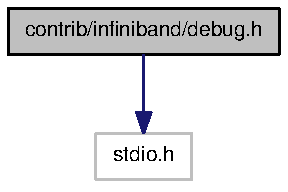
\includegraphics[width=87pt]{debug_8h__incl}
\end{center}
\end{figure}
このグラフは、どのファイルから直接、間接的にインクルードされているかを示しています。\nopagebreak
\begin{figure}[H]
\begin{center}
\leavevmode
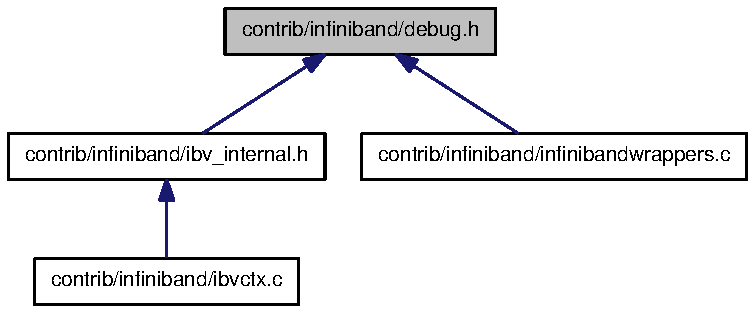
\includegraphics[width=199pt]{debug_8h__dep__incl}
\end{center}
\end{figure}
\subsection*{マクロ定義}
\begin{DoxyCompactItemize}
\item 
\#define \hyperlink{debug_8h_a5a9cc968ee7262fddda93f73341beedb}{PDEBUG}(fmt, args...)~printf(fmt, \#\#args)
\end{DoxyCompactItemize}


\subsection{マクロ定義}
\hypertarget{debug_8h_a5a9cc968ee7262fddda93f73341beedb}{
\index{debug.h@{debug.h}!PDEBUG@{PDEBUG}}
\index{PDEBUG@{PDEBUG}!debug.h@{debug.h}}
\subsubsection[{PDEBUG}]{\setlength{\rightskip}{0pt plus 5cm}\#define PDEBUG(fmt, \/  args...)~printf(fmt, \#\#args)}}
\label{debug_8h_a5a9cc968ee7262fddda93f73341beedb}

\hypertarget{dmtcpinterface_8h}{
\section{contrib/infiniband/dmtcpinterface.h}
\label{dmtcpinterface_8h}\index{contrib/infiniband/dmtcpinterface.h@{contrib/infiniband/dmtcpinterface.h}}
}
\subsection*{型定義}
\begin{DoxyCompactItemize}
\item 
typedef enum \hyperlink{dmtcpinterface_8h_ae62746d6da653108d183b6261c2101a7}{eDmtcpEvent} \hyperlink{dmtcpinterface_8h_a1a2facd3d07dcfbe546435a70edb61ac}{DmtcpEvent\_\-t}
\end{DoxyCompactItemize}
\subsection*{列挙型}
\begin{DoxyCompactItemize}
\item 
enum \hyperlink{dmtcpinterface_8h_ae62746d6da653108d183b6261c2101a7}{eDmtcpEvent} \{ \par
\hyperlink{dmtcpinterface_8h_ae62746d6da653108d183b6261c2101a7a5802c6a097c357228e1fb6eee7384113}{DMTCP\_\-EVENT\_\-INIT}, 
\hyperlink{dmtcpinterface_8h_ae62746d6da653108d183b6261c2101a7a49c41359bfeb759726802faeb41eb5e5}{DMTCP\_\-EVENT\_\-PRE\_\-EXIT}, 
\hyperlink{dmtcpinterface_8h_ae62746d6da653108d183b6261c2101a7a72b772b022beee9e49f6d5d1cc201831}{DMTCP\_\-EVENT\_\-RESET\_\-ON\_\-FORK}, 
\hyperlink{dmtcpinterface_8h_ae62746d6da653108d183b6261c2101a7a69dc96516935b8fa4178148e9eb2090e}{DMTCP\_\-EVENT\_\-POST\_\-SUSPEND}, 
\par
\hyperlink{dmtcpinterface_8h_ae62746d6da653108d183b6261c2101a7a6bab469784ea4fc38e6a1a1d4df0c36e}{DMTCP\_\-EVENT\_\-POST\_\-LEADER\_\-ELECTION}, 
\hyperlink{dmtcpinterface_8h_ae62746d6da653108d183b6261c2101a7a16b7fe325c2b6fb816df949279001c95}{DMTCP\_\-EVENT\_\-POST\_\-DRAIN}, 
\hyperlink{dmtcpinterface_8h_ae62746d6da653108d183b6261c2101a7a562fded7e3eb48e96b65074416915053}{DMTCP\_\-EVENT\_\-PRE\_\-CHECKPOINT}, 
\hyperlink{dmtcpinterface_8h_ae62746d6da653108d183b6261c2101a7a0dd2e11f6c9017cf0b34ab5ba9df84e3}{DMTCP\_\-EVENT\_\-POST\_\-CHECKPOINT}, 
\par
\hyperlink{dmtcpinterface_8h_ae62746d6da653108d183b6261c2101a7a2e8f871534696a5dbb9366089616189d}{DMTCP\_\-EVENT\_\-REGISTER\_\-NAME\_\-SERVICE\_\-DATA}, 
\hyperlink{dmtcpinterface_8h_ae62746d6da653108d183b6261c2101a7a5935dc50bfb92475305d652e834bf630}{DMTCP\_\-EVENT\_\-SEND\_\-QUERIES}, 
\hyperlink{dmtcpinterface_8h_ae62746d6da653108d183b6261c2101a7acc0f23d5fab62a8e8420ffdc81fd1f05}{DMTCP\_\-EVENT\_\-POST\_\-CHECKPOINT\_\-RESUME}, 
\hyperlink{dmtcpinterface_8h_ae62746d6da653108d183b6261c2101a7a02ef977716ca74dcd29cdd6991cadc57}{DMTCP\_\-EVENT\_\-POST\_\-RESTART}, 
\par
\hyperlink{dmtcpinterface_8h_ae62746d6da653108d183b6261c2101a7a60a5f43e0413ef9431bc03dd501536f0}{DMTCP\_\-EVENT\_\-POST\_\-RESTART\_\-RESUME}, 
\hyperlink{dmtcpinterface_8h_ae62746d6da653108d183b6261c2101a7a81e40f4c706a18c7738b48361dbe8135}{nDmtcpEvents}, 
\hyperlink{dmtcp_8h_ae62746d6da653108d183b6261c2101a7a5802c6a097c357228e1fb6eee7384113}{DMTCP\_\-EVENT\_\-INIT}, 
\hyperlink{dmtcp_8h_ae62746d6da653108d183b6261c2101a7ad026c4c7891b6c62228630baab62c504}{DMTCP\_\-EVENT\_\-EXIT}, 
\par
\hyperlink{dmtcp_8h_ae62746d6da653108d183b6261c2101a7a4cad9cbca1d6205cf9da037bacb570dd}{DMTCP\_\-EVENT\_\-PRE\_\-EXEC}, 
\hyperlink{dmtcp_8h_ae62746d6da653108d183b6261c2101a7a9d1b0cac0f6e185d69db9962d481b850}{DMTCP\_\-EVENT\_\-POST\_\-EXEC}, 
\hyperlink{dmtcp_8h_ae62746d6da653108d183b6261c2101a7ae48b2c31aa2393e6ff04f212ae21fdca}{DMTCP\_\-EVENT\_\-ATFORK\_\-PREPARE}, 
\hyperlink{dmtcp_8h_ae62746d6da653108d183b6261c2101a7aafd48068ab9bd15e3f6271a70f413d64}{DMTCP\_\-EVENT\_\-ATFORK\_\-PARENT}, 
\par
\hyperlink{dmtcp_8h_ae62746d6da653108d183b6261c2101a7a497a4841781baf6e1e18a90f410e780b}{DMTCP\_\-EVENT\_\-ATFORK\_\-CHILD}, 
\hyperlink{dmtcp_8h_ae62746d6da653108d183b6261c2101a7ad5272eed974d56fb0e60b1bb300216f9}{DMTCP\_\-EVENT\_\-WAIT\_\-FOR\_\-SUSPEND\_\-MSG}, 
\hyperlink{dmtcp_8h_ae62746d6da653108d183b6261c2101a7a95d43100d4260cf6206f8d827496633b}{DMTCP\_\-EVENT\_\-THREADS\_\-SUSPEND}, 
\hyperlink{dmtcp_8h_ae62746d6da653108d183b6261c2101a7a9e68e0439c03713525bc4cef79dacb42}{DMTCP\_\-EVENT\_\-LEADER\_\-ELECTION}, 
\par
\hyperlink{dmtcp_8h_ae62746d6da653108d183b6261c2101a7ad2390fea85c9ccc4646c2267b9592538}{DMTCP\_\-EVENT\_\-DRAIN}, 
\hyperlink{dmtcp_8h_ae62746d6da653108d183b6261c2101a7ab64f8bdd4e9c6af6aba14bcd241f72c5}{DMTCP\_\-EVENT\_\-WRITE\_\-CKPT}, 
\hyperlink{dmtcp_8h_ae62746d6da653108d183b6261c2101a7ac1a9995c30746a802abb9e9f85211891}{DMTCP\_\-EVENT\_\-RESTART}, 
\hyperlink{dmtcp_8h_ae62746d6da653108d183b6261c2101a7ac4209272d6edeb6eca94aab06754fcf3}{DMTCP\_\-EVENT\_\-RESUME}, 
\par
\hyperlink{dmtcp_8h_ae62746d6da653108d183b6261c2101a7a2e8f871534696a5dbb9366089616189d}{DMTCP\_\-EVENT\_\-REGISTER\_\-NAME\_\-SERVICE\_\-DATA}, 
\hyperlink{dmtcp_8h_ae62746d6da653108d183b6261c2101a7a5935dc50bfb92475305d652e834bf630}{DMTCP\_\-EVENT\_\-SEND\_\-QUERIES}, 
\hyperlink{dmtcp_8h_ae62746d6da653108d183b6261c2101a7a9199507b677d6b0a7dc50d967b866e5f}{DMTCP\_\-EVENT\_\-REFILL}, 
\hyperlink{dmtcp_8h_ae62746d6da653108d183b6261c2101a7a9dbb8b43a3af9d2c80e4126423490f3c}{DMTCP\_\-EVENT\_\-THREADS\_\-RESUME}, 
\par
\hyperlink{dmtcp_8h_ae62746d6da653108d183b6261c2101a7a353b86ad0397eb40faa4c955853bb498}{DMTCP\_\-EVENT\_\-PRE\_\-SUSPEND\_\-USER\_\-THREAD}, 
\hyperlink{dmtcp_8h_ae62746d6da653108d183b6261c2101a7a28e4048dcd385df9f907fef9bd698623}{DMTCP\_\-EVENT\_\-RESUME\_\-USER\_\-THREAD}, 
\hyperlink{dmtcp_8h_ae62746d6da653108d183b6261c2101a7afffc5b019dd7a7d3ca99b4c797e4ded6}{DMTCP\_\-EVENT\_\-THREAD\_\-START}, 
\hyperlink{dmtcp_8h_ae62746d6da653108d183b6261c2101a7a4a0753d61b2c2aa71b3ad951f0a35b07}{DMTCP\_\-EVENT\_\-THREAD\_\-CREATED}, 
\par
\hyperlink{dmtcp_8h_ae62746d6da653108d183b6261c2101a7abbb13958669391068e351c9af85805f3}{DMTCP\_\-EVENT\_\-PTHREAD\_\-START}, 
\hyperlink{dmtcp_8h_ae62746d6da653108d183b6261c2101a7a0917c5b450b2844b6090913940cef74c}{DMTCP\_\-EVENT\_\-PTHREAD\_\-EXIT}, 
\hyperlink{dmtcp_8h_ae62746d6da653108d183b6261c2101a7a6d6168617d3af70a4152b176a43c9f7e}{DMTCP\_\-EVENT\_\-PTHREAD\_\-RETURN}, 
\hyperlink{dmtcp_8h_ae62746d6da653108d183b6261c2101a7a81e40f4c706a18c7738b48361dbe8135}{nDmtcpEvents}
 \}
\end{DoxyCompactItemize}
\subsection*{関数}
\begin{DoxyCompactItemize}
\item 
void \hyperlink{dmtcpinterface_8h_ab84d885ac90fd3a2490f353906df9548}{process\_\-dmtcp\_\-event} (\hyperlink{dmtcp_8h_a1a2facd3d07dcfbe546435a70edb61ac}{DmtcpEvent\_\-t} event, void $\ast$data)
\item 
int \hyperlink{dmtcpinterface_8h_a586917e27ae1ef796f9a1d3632f1fc84}{dmtcp\_\-get\_\-ckpt\_\-signal} ()
\item 
const char $\ast$ \hyperlink{dmtcpinterface_8h_a566b789c5968c2e760171ac01dbb6d91}{dmtcp\_\-get\_\-tmpdir} ()
\item 
const char $\ast$ \hyperlink{dmtcpinterface_8h_ad66efb25452c3dc520dc0aef3b126543}{dmtcp\_\-get\_\-uniquepid\_\-str} ()
\item 
int \hyperlink{dmtcpinterface_8h_a63b295126a98768b49e59652a5856031}{dmtcp\_\-is\_\-running\_\-state} ()
\end{DoxyCompactItemize}


\subsection{型定義}
\hypertarget{dmtcpinterface_8h_a1a2facd3d07dcfbe546435a70edb61ac}{
\index{dmtcpinterface.h@{dmtcpinterface.h}!DmtcpEvent\_\-t@{DmtcpEvent\_\-t}}
\index{DmtcpEvent\_\-t@{DmtcpEvent\_\-t}!dmtcpinterface.h@{dmtcpinterface.h}}
\subsubsection[{DmtcpEvent\_\-t}]{\setlength{\rightskip}{0pt plus 5cm}typedef enum {\bf eDmtcpEvent}  {\bf DmtcpEvent\_\-t}}}
\label{dmtcpinterface_8h_a1a2facd3d07dcfbe546435a70edb61ac}


\subsection{列挙型}
\hypertarget{dmtcpinterface_8h_ae62746d6da653108d183b6261c2101a7}{
\index{dmtcpinterface.h@{dmtcpinterface.h}!eDmtcpEvent@{eDmtcpEvent}}
\index{eDmtcpEvent@{eDmtcpEvent}!dmtcpinterface.h@{dmtcpinterface.h}}
\subsubsection[{eDmtcpEvent}]{\setlength{\rightskip}{0pt plus 5cm}enum {\bf eDmtcpEvent}}}
\label{dmtcpinterface_8h_ae62746d6da653108d183b6261c2101a7}
\begin{Desc}
\item[列挙型の値: ]\par
\begin{description}
\index{DMTCP\_\-EVENT\_\-INIT@{DMTCP\_\-EVENT\_\-INIT}!dmtcpinterface.h@{dmtcpinterface.h}}\index{dmtcpinterface.h@{dmtcpinterface.h}!DMTCP\_\-EVENT\_\-INIT@{DMTCP\_\-EVENT\_\-INIT}}\item[{\em 
\hypertarget{dmtcpinterface_8h_ae62746d6da653108d183b6261c2101a7a5802c6a097c357228e1fb6eee7384113}{
DMTCP\_\-EVENT\_\-INIT}
\label{dmtcpinterface_8h_ae62746d6da653108d183b6261c2101a7a5802c6a097c357228e1fb6eee7384113}
}]\index{DMTCP\_\-EVENT\_\-PRE\_\-EXIT@{DMTCP\_\-EVENT\_\-PRE\_\-EXIT}!dmtcpinterface.h@{dmtcpinterface.h}}\index{dmtcpinterface.h@{dmtcpinterface.h}!DMTCP\_\-EVENT\_\-PRE\_\-EXIT@{DMTCP\_\-EVENT\_\-PRE\_\-EXIT}}\item[{\em 
\hypertarget{dmtcpinterface_8h_ae62746d6da653108d183b6261c2101a7a49c41359bfeb759726802faeb41eb5e5}{
DMTCP\_\-EVENT\_\-PRE\_\-EXIT}
\label{dmtcpinterface_8h_ae62746d6da653108d183b6261c2101a7a49c41359bfeb759726802faeb41eb5e5}
}]\index{DMTCP\_\-EVENT\_\-RESET\_\-ON\_\-FORK@{DMTCP\_\-EVENT\_\-RESET\_\-ON\_\-FORK}!dmtcpinterface.h@{dmtcpinterface.h}}\index{dmtcpinterface.h@{dmtcpinterface.h}!DMTCP\_\-EVENT\_\-RESET\_\-ON\_\-FORK@{DMTCP\_\-EVENT\_\-RESET\_\-ON\_\-FORK}}\item[{\em 
\hypertarget{dmtcpinterface_8h_ae62746d6da653108d183b6261c2101a7a72b772b022beee9e49f6d5d1cc201831}{
DMTCP\_\-EVENT\_\-RESET\_\-ON\_\-FORK}
\label{dmtcpinterface_8h_ae62746d6da653108d183b6261c2101a7a72b772b022beee9e49f6d5d1cc201831}
}]\index{DMTCP\_\-EVENT\_\-POST\_\-SUSPEND@{DMTCP\_\-EVENT\_\-POST\_\-SUSPEND}!dmtcpinterface.h@{dmtcpinterface.h}}\index{dmtcpinterface.h@{dmtcpinterface.h}!DMTCP\_\-EVENT\_\-POST\_\-SUSPEND@{DMTCP\_\-EVENT\_\-POST\_\-SUSPEND}}\item[{\em 
\hypertarget{dmtcpinterface_8h_ae62746d6da653108d183b6261c2101a7a69dc96516935b8fa4178148e9eb2090e}{
DMTCP\_\-EVENT\_\-POST\_\-SUSPEND}
\label{dmtcpinterface_8h_ae62746d6da653108d183b6261c2101a7a69dc96516935b8fa4178148e9eb2090e}
}]\index{DMTCP\_\-EVENT\_\-POST\_\-LEADER\_\-ELECTION@{DMTCP\_\-EVENT\_\-POST\_\-LEADER\_\-ELECTION}!dmtcpinterface.h@{dmtcpinterface.h}}\index{dmtcpinterface.h@{dmtcpinterface.h}!DMTCP\_\-EVENT\_\-POST\_\-LEADER\_\-ELECTION@{DMTCP\_\-EVENT\_\-POST\_\-LEADER\_\-ELECTION}}\item[{\em 
\hypertarget{dmtcpinterface_8h_ae62746d6da653108d183b6261c2101a7a6bab469784ea4fc38e6a1a1d4df0c36e}{
DMTCP\_\-EVENT\_\-POST\_\-LEADER\_\-ELECTION}
\label{dmtcpinterface_8h_ae62746d6da653108d183b6261c2101a7a6bab469784ea4fc38e6a1a1d4df0c36e}
}]\index{DMTCP\_\-EVENT\_\-POST\_\-DRAIN@{DMTCP\_\-EVENT\_\-POST\_\-DRAIN}!dmtcpinterface.h@{dmtcpinterface.h}}\index{dmtcpinterface.h@{dmtcpinterface.h}!DMTCP\_\-EVENT\_\-POST\_\-DRAIN@{DMTCP\_\-EVENT\_\-POST\_\-DRAIN}}\item[{\em 
\hypertarget{dmtcpinterface_8h_ae62746d6da653108d183b6261c2101a7a16b7fe325c2b6fb816df949279001c95}{
DMTCP\_\-EVENT\_\-POST\_\-DRAIN}
\label{dmtcpinterface_8h_ae62746d6da653108d183b6261c2101a7a16b7fe325c2b6fb816df949279001c95}
}]\index{DMTCP\_\-EVENT\_\-PRE\_\-CHECKPOINT@{DMTCP\_\-EVENT\_\-PRE\_\-CHECKPOINT}!dmtcpinterface.h@{dmtcpinterface.h}}\index{dmtcpinterface.h@{dmtcpinterface.h}!DMTCP\_\-EVENT\_\-PRE\_\-CHECKPOINT@{DMTCP\_\-EVENT\_\-PRE\_\-CHECKPOINT}}\item[{\em 
\hypertarget{dmtcpinterface_8h_ae62746d6da653108d183b6261c2101a7a562fded7e3eb48e96b65074416915053}{
DMTCP\_\-EVENT\_\-PRE\_\-CHECKPOINT}
\label{dmtcpinterface_8h_ae62746d6da653108d183b6261c2101a7a562fded7e3eb48e96b65074416915053}
}]\index{DMTCP\_\-EVENT\_\-POST\_\-CHECKPOINT@{DMTCP\_\-EVENT\_\-POST\_\-CHECKPOINT}!dmtcpinterface.h@{dmtcpinterface.h}}\index{dmtcpinterface.h@{dmtcpinterface.h}!DMTCP\_\-EVENT\_\-POST\_\-CHECKPOINT@{DMTCP\_\-EVENT\_\-POST\_\-CHECKPOINT}}\item[{\em 
\hypertarget{dmtcpinterface_8h_ae62746d6da653108d183b6261c2101a7a0dd2e11f6c9017cf0b34ab5ba9df84e3}{
DMTCP\_\-EVENT\_\-POST\_\-CHECKPOINT}
\label{dmtcpinterface_8h_ae62746d6da653108d183b6261c2101a7a0dd2e11f6c9017cf0b34ab5ba9df84e3}
}]\index{DMTCP\_\-EVENT\_\-REGISTER\_\-NAME\_\-SERVICE\_\-DATA@{DMTCP\_\-EVENT\_\-REGISTER\_\-NAME\_\-SERVICE\_\-DATA}!dmtcpinterface.h@{dmtcpinterface.h}}\index{dmtcpinterface.h@{dmtcpinterface.h}!DMTCP\_\-EVENT\_\-REGISTER\_\-NAME\_\-SERVICE\_\-DATA@{DMTCP\_\-EVENT\_\-REGISTER\_\-NAME\_\-SERVICE\_\-DATA}}\item[{\em 
\hypertarget{dmtcpinterface_8h_ae62746d6da653108d183b6261c2101a7a2e8f871534696a5dbb9366089616189d}{
DMTCP\_\-EVENT\_\-REGISTER\_\-NAME\_\-SERVICE\_\-DATA}
\label{dmtcpinterface_8h_ae62746d6da653108d183b6261c2101a7a2e8f871534696a5dbb9366089616189d}
}]\index{DMTCP\_\-EVENT\_\-SEND\_\-QUERIES@{DMTCP\_\-EVENT\_\-SEND\_\-QUERIES}!dmtcpinterface.h@{dmtcpinterface.h}}\index{dmtcpinterface.h@{dmtcpinterface.h}!DMTCP\_\-EVENT\_\-SEND\_\-QUERIES@{DMTCP\_\-EVENT\_\-SEND\_\-QUERIES}}\item[{\em 
\hypertarget{dmtcpinterface_8h_ae62746d6da653108d183b6261c2101a7a5935dc50bfb92475305d652e834bf630}{
DMTCP\_\-EVENT\_\-SEND\_\-QUERIES}
\label{dmtcpinterface_8h_ae62746d6da653108d183b6261c2101a7a5935dc50bfb92475305d652e834bf630}
}]\index{DMTCP\_\-EVENT\_\-POST\_\-CHECKPOINT\_\-RESUME@{DMTCP\_\-EVENT\_\-POST\_\-CHECKPOINT\_\-RESUME}!dmtcpinterface.h@{dmtcpinterface.h}}\index{dmtcpinterface.h@{dmtcpinterface.h}!DMTCP\_\-EVENT\_\-POST\_\-CHECKPOINT\_\-RESUME@{DMTCP\_\-EVENT\_\-POST\_\-CHECKPOINT\_\-RESUME}}\item[{\em 
\hypertarget{dmtcpinterface_8h_ae62746d6da653108d183b6261c2101a7acc0f23d5fab62a8e8420ffdc81fd1f05}{
DMTCP\_\-EVENT\_\-POST\_\-CHECKPOINT\_\-RESUME}
\label{dmtcpinterface_8h_ae62746d6da653108d183b6261c2101a7acc0f23d5fab62a8e8420ffdc81fd1f05}
}]\index{DMTCP\_\-EVENT\_\-POST\_\-RESTART@{DMTCP\_\-EVENT\_\-POST\_\-RESTART}!dmtcpinterface.h@{dmtcpinterface.h}}\index{dmtcpinterface.h@{dmtcpinterface.h}!DMTCP\_\-EVENT\_\-POST\_\-RESTART@{DMTCP\_\-EVENT\_\-POST\_\-RESTART}}\item[{\em 
\hypertarget{dmtcpinterface_8h_ae62746d6da653108d183b6261c2101a7a02ef977716ca74dcd29cdd6991cadc57}{
DMTCP\_\-EVENT\_\-POST\_\-RESTART}
\label{dmtcpinterface_8h_ae62746d6da653108d183b6261c2101a7a02ef977716ca74dcd29cdd6991cadc57}
}]\index{DMTCP\_\-EVENT\_\-POST\_\-RESTART\_\-RESUME@{DMTCP\_\-EVENT\_\-POST\_\-RESTART\_\-RESUME}!dmtcpinterface.h@{dmtcpinterface.h}}\index{dmtcpinterface.h@{dmtcpinterface.h}!DMTCP\_\-EVENT\_\-POST\_\-RESTART\_\-RESUME@{DMTCP\_\-EVENT\_\-POST\_\-RESTART\_\-RESUME}}\item[{\em 
\hypertarget{dmtcpinterface_8h_ae62746d6da653108d183b6261c2101a7a60a5f43e0413ef9431bc03dd501536f0}{
DMTCP\_\-EVENT\_\-POST\_\-RESTART\_\-RESUME}
\label{dmtcpinterface_8h_ae62746d6da653108d183b6261c2101a7a60a5f43e0413ef9431bc03dd501536f0}
}]\index{nDmtcpEvents@{nDmtcpEvents}!dmtcpinterface.h@{dmtcpinterface.h}}\index{dmtcpinterface.h@{dmtcpinterface.h}!nDmtcpEvents@{nDmtcpEvents}}\item[{\em 
\hypertarget{dmtcpinterface_8h_ae62746d6da653108d183b6261c2101a7a81e40f4c706a18c7738b48361dbe8135}{
nDmtcpEvents}
\label{dmtcpinterface_8h_ae62746d6da653108d183b6261c2101a7a81e40f4c706a18c7738b48361dbe8135}
}]\index{DMTCP\_\-EVENT\_\-INIT@{DMTCP\_\-EVENT\_\-INIT}!dmtcpinterface.h@{dmtcpinterface.h}}\index{dmtcpinterface.h@{dmtcpinterface.h}!DMTCP\_\-EVENT\_\-INIT@{DMTCP\_\-EVENT\_\-INIT}}\item[{\em 
\hypertarget{dmtcpinterface_8h_ae62746d6da653108d183b6261c2101a7a5802c6a097c357228e1fb6eee7384113}{
DMTCP\_\-EVENT\_\-INIT}
\label{dmtcpinterface_8h_ae62746d6da653108d183b6261c2101a7a5802c6a097c357228e1fb6eee7384113}
}]\index{DMTCP\_\-EVENT\_\-EXIT@{DMTCP\_\-EVENT\_\-EXIT}!dmtcpinterface.h@{dmtcpinterface.h}}\index{dmtcpinterface.h@{dmtcpinterface.h}!DMTCP\_\-EVENT\_\-EXIT@{DMTCP\_\-EVENT\_\-EXIT}}\item[{\em 
\hypertarget{dmtcpinterface_8h_ae62746d6da653108d183b6261c2101a7ad026c4c7891b6c62228630baab62c504}{
DMTCP\_\-EVENT\_\-EXIT}
\label{dmtcpinterface_8h_ae62746d6da653108d183b6261c2101a7ad026c4c7891b6c62228630baab62c504}
}]\index{DMTCP\_\-EVENT\_\-PRE\_\-EXEC@{DMTCP\_\-EVENT\_\-PRE\_\-EXEC}!dmtcpinterface.h@{dmtcpinterface.h}}\index{dmtcpinterface.h@{dmtcpinterface.h}!DMTCP\_\-EVENT\_\-PRE\_\-EXEC@{DMTCP\_\-EVENT\_\-PRE\_\-EXEC}}\item[{\em 
\hypertarget{dmtcpinterface_8h_ae62746d6da653108d183b6261c2101a7a4cad9cbca1d6205cf9da037bacb570dd}{
DMTCP\_\-EVENT\_\-PRE\_\-EXEC}
\label{dmtcpinterface_8h_ae62746d6da653108d183b6261c2101a7a4cad9cbca1d6205cf9da037bacb570dd}
}]\index{DMTCP\_\-EVENT\_\-POST\_\-EXEC@{DMTCP\_\-EVENT\_\-POST\_\-EXEC}!dmtcpinterface.h@{dmtcpinterface.h}}\index{dmtcpinterface.h@{dmtcpinterface.h}!DMTCP\_\-EVENT\_\-POST\_\-EXEC@{DMTCP\_\-EVENT\_\-POST\_\-EXEC}}\item[{\em 
\hypertarget{dmtcpinterface_8h_ae62746d6da653108d183b6261c2101a7a9d1b0cac0f6e185d69db9962d481b850}{
DMTCP\_\-EVENT\_\-POST\_\-EXEC}
\label{dmtcpinterface_8h_ae62746d6da653108d183b6261c2101a7a9d1b0cac0f6e185d69db9962d481b850}
}]\index{DMTCP\_\-EVENT\_\-ATFORK\_\-PREPARE@{DMTCP\_\-EVENT\_\-ATFORK\_\-PREPARE}!dmtcpinterface.h@{dmtcpinterface.h}}\index{dmtcpinterface.h@{dmtcpinterface.h}!DMTCP\_\-EVENT\_\-ATFORK\_\-PREPARE@{DMTCP\_\-EVENT\_\-ATFORK\_\-PREPARE}}\item[{\em 
\hypertarget{dmtcpinterface_8h_ae62746d6da653108d183b6261c2101a7ae48b2c31aa2393e6ff04f212ae21fdca}{
DMTCP\_\-EVENT\_\-ATFORK\_\-PREPARE}
\label{dmtcpinterface_8h_ae62746d6da653108d183b6261c2101a7ae48b2c31aa2393e6ff04f212ae21fdca}
}]\index{DMTCP\_\-EVENT\_\-ATFORK\_\-PARENT@{DMTCP\_\-EVENT\_\-ATFORK\_\-PARENT}!dmtcpinterface.h@{dmtcpinterface.h}}\index{dmtcpinterface.h@{dmtcpinterface.h}!DMTCP\_\-EVENT\_\-ATFORK\_\-PARENT@{DMTCP\_\-EVENT\_\-ATFORK\_\-PARENT}}\item[{\em 
\hypertarget{dmtcpinterface_8h_ae62746d6da653108d183b6261c2101a7aafd48068ab9bd15e3f6271a70f413d64}{
DMTCP\_\-EVENT\_\-ATFORK\_\-PARENT}
\label{dmtcpinterface_8h_ae62746d6da653108d183b6261c2101a7aafd48068ab9bd15e3f6271a70f413d64}
}]\index{DMTCP\_\-EVENT\_\-ATFORK\_\-CHILD@{DMTCP\_\-EVENT\_\-ATFORK\_\-CHILD}!dmtcpinterface.h@{dmtcpinterface.h}}\index{dmtcpinterface.h@{dmtcpinterface.h}!DMTCP\_\-EVENT\_\-ATFORK\_\-CHILD@{DMTCP\_\-EVENT\_\-ATFORK\_\-CHILD}}\item[{\em 
\hypertarget{dmtcpinterface_8h_ae62746d6da653108d183b6261c2101a7a497a4841781baf6e1e18a90f410e780b}{
DMTCP\_\-EVENT\_\-ATFORK\_\-CHILD}
\label{dmtcpinterface_8h_ae62746d6da653108d183b6261c2101a7a497a4841781baf6e1e18a90f410e780b}
}]\index{DMTCP\_\-EVENT\_\-WAIT\_\-FOR\_\-SUSPEND\_\-MSG@{DMTCP\_\-EVENT\_\-WAIT\_\-FOR\_\-SUSPEND\_\-MSG}!dmtcpinterface.h@{dmtcpinterface.h}}\index{dmtcpinterface.h@{dmtcpinterface.h}!DMTCP\_\-EVENT\_\-WAIT\_\-FOR\_\-SUSPEND\_\-MSG@{DMTCP\_\-EVENT\_\-WAIT\_\-FOR\_\-SUSPEND\_\-MSG}}\item[{\em 
\hypertarget{dmtcpinterface_8h_ae62746d6da653108d183b6261c2101a7ad5272eed974d56fb0e60b1bb300216f9}{
DMTCP\_\-EVENT\_\-WAIT\_\-FOR\_\-SUSPEND\_\-MSG}
\label{dmtcpinterface_8h_ae62746d6da653108d183b6261c2101a7ad5272eed974d56fb0e60b1bb300216f9}
}]\index{DMTCP\_\-EVENT\_\-THREADS\_\-SUSPEND@{DMTCP\_\-EVENT\_\-THREADS\_\-SUSPEND}!dmtcpinterface.h@{dmtcpinterface.h}}\index{dmtcpinterface.h@{dmtcpinterface.h}!DMTCP\_\-EVENT\_\-THREADS\_\-SUSPEND@{DMTCP\_\-EVENT\_\-THREADS\_\-SUSPEND}}\item[{\em 
\hypertarget{dmtcpinterface_8h_ae62746d6da653108d183b6261c2101a7a95d43100d4260cf6206f8d827496633b}{
DMTCP\_\-EVENT\_\-THREADS\_\-SUSPEND}
\label{dmtcpinterface_8h_ae62746d6da653108d183b6261c2101a7a95d43100d4260cf6206f8d827496633b}
}]\index{DMTCP\_\-EVENT\_\-LEADER\_\-ELECTION@{DMTCP\_\-EVENT\_\-LEADER\_\-ELECTION}!dmtcpinterface.h@{dmtcpinterface.h}}\index{dmtcpinterface.h@{dmtcpinterface.h}!DMTCP\_\-EVENT\_\-LEADER\_\-ELECTION@{DMTCP\_\-EVENT\_\-LEADER\_\-ELECTION}}\item[{\em 
\hypertarget{dmtcpinterface_8h_ae62746d6da653108d183b6261c2101a7a9e68e0439c03713525bc4cef79dacb42}{
DMTCP\_\-EVENT\_\-LEADER\_\-ELECTION}
\label{dmtcpinterface_8h_ae62746d6da653108d183b6261c2101a7a9e68e0439c03713525bc4cef79dacb42}
}]\index{DMTCP\_\-EVENT\_\-DRAIN@{DMTCP\_\-EVENT\_\-DRAIN}!dmtcpinterface.h@{dmtcpinterface.h}}\index{dmtcpinterface.h@{dmtcpinterface.h}!DMTCP\_\-EVENT\_\-DRAIN@{DMTCP\_\-EVENT\_\-DRAIN}}\item[{\em 
\hypertarget{dmtcpinterface_8h_ae62746d6da653108d183b6261c2101a7ad2390fea85c9ccc4646c2267b9592538}{
DMTCP\_\-EVENT\_\-DRAIN}
\label{dmtcpinterface_8h_ae62746d6da653108d183b6261c2101a7ad2390fea85c9ccc4646c2267b9592538}
}]\index{DMTCP\_\-EVENT\_\-WRITE\_\-CKPT@{DMTCP\_\-EVENT\_\-WRITE\_\-CKPT}!dmtcpinterface.h@{dmtcpinterface.h}}\index{dmtcpinterface.h@{dmtcpinterface.h}!DMTCP\_\-EVENT\_\-WRITE\_\-CKPT@{DMTCP\_\-EVENT\_\-WRITE\_\-CKPT}}\item[{\em 
\hypertarget{dmtcpinterface_8h_ae62746d6da653108d183b6261c2101a7ab64f8bdd4e9c6af6aba14bcd241f72c5}{
DMTCP\_\-EVENT\_\-WRITE\_\-CKPT}
\label{dmtcpinterface_8h_ae62746d6da653108d183b6261c2101a7ab64f8bdd4e9c6af6aba14bcd241f72c5}
}]\index{DMTCP\_\-EVENT\_\-RESTART@{DMTCP\_\-EVENT\_\-RESTART}!dmtcpinterface.h@{dmtcpinterface.h}}\index{dmtcpinterface.h@{dmtcpinterface.h}!DMTCP\_\-EVENT\_\-RESTART@{DMTCP\_\-EVENT\_\-RESTART}}\item[{\em 
\hypertarget{dmtcpinterface_8h_ae62746d6da653108d183b6261c2101a7ac1a9995c30746a802abb9e9f85211891}{
DMTCP\_\-EVENT\_\-RESTART}
\label{dmtcpinterface_8h_ae62746d6da653108d183b6261c2101a7ac1a9995c30746a802abb9e9f85211891}
}]\index{DMTCP\_\-EVENT\_\-RESUME@{DMTCP\_\-EVENT\_\-RESUME}!dmtcpinterface.h@{dmtcpinterface.h}}\index{dmtcpinterface.h@{dmtcpinterface.h}!DMTCP\_\-EVENT\_\-RESUME@{DMTCP\_\-EVENT\_\-RESUME}}\item[{\em 
\hypertarget{dmtcpinterface_8h_ae62746d6da653108d183b6261c2101a7ac4209272d6edeb6eca94aab06754fcf3}{
DMTCP\_\-EVENT\_\-RESUME}
\label{dmtcpinterface_8h_ae62746d6da653108d183b6261c2101a7ac4209272d6edeb6eca94aab06754fcf3}
}]\index{DMTCP\_\-EVENT\_\-REGISTER\_\-NAME\_\-SERVICE\_\-DATA@{DMTCP\_\-EVENT\_\-REGISTER\_\-NAME\_\-SERVICE\_\-DATA}!dmtcpinterface.h@{dmtcpinterface.h}}\index{dmtcpinterface.h@{dmtcpinterface.h}!DMTCP\_\-EVENT\_\-REGISTER\_\-NAME\_\-SERVICE\_\-DATA@{DMTCP\_\-EVENT\_\-REGISTER\_\-NAME\_\-SERVICE\_\-DATA}}\item[{\em 
\hypertarget{dmtcpinterface_8h_ae62746d6da653108d183b6261c2101a7a2e8f871534696a5dbb9366089616189d}{
DMTCP\_\-EVENT\_\-REGISTER\_\-NAME\_\-SERVICE\_\-DATA}
\label{dmtcpinterface_8h_ae62746d6da653108d183b6261c2101a7a2e8f871534696a5dbb9366089616189d}
}]\index{DMTCP\_\-EVENT\_\-SEND\_\-QUERIES@{DMTCP\_\-EVENT\_\-SEND\_\-QUERIES}!dmtcpinterface.h@{dmtcpinterface.h}}\index{dmtcpinterface.h@{dmtcpinterface.h}!DMTCP\_\-EVENT\_\-SEND\_\-QUERIES@{DMTCP\_\-EVENT\_\-SEND\_\-QUERIES}}\item[{\em 
\hypertarget{dmtcpinterface_8h_ae62746d6da653108d183b6261c2101a7a5935dc50bfb92475305d652e834bf630}{
DMTCP\_\-EVENT\_\-SEND\_\-QUERIES}
\label{dmtcpinterface_8h_ae62746d6da653108d183b6261c2101a7a5935dc50bfb92475305d652e834bf630}
}]\index{DMTCP\_\-EVENT\_\-REFILL@{DMTCP\_\-EVENT\_\-REFILL}!dmtcpinterface.h@{dmtcpinterface.h}}\index{dmtcpinterface.h@{dmtcpinterface.h}!DMTCP\_\-EVENT\_\-REFILL@{DMTCP\_\-EVENT\_\-REFILL}}\item[{\em 
\hypertarget{dmtcpinterface_8h_ae62746d6da653108d183b6261c2101a7a9199507b677d6b0a7dc50d967b866e5f}{
DMTCP\_\-EVENT\_\-REFILL}
\label{dmtcpinterface_8h_ae62746d6da653108d183b6261c2101a7a9199507b677d6b0a7dc50d967b866e5f}
}]\index{DMTCP\_\-EVENT\_\-THREADS\_\-RESUME@{DMTCP\_\-EVENT\_\-THREADS\_\-RESUME}!dmtcpinterface.h@{dmtcpinterface.h}}\index{dmtcpinterface.h@{dmtcpinterface.h}!DMTCP\_\-EVENT\_\-THREADS\_\-RESUME@{DMTCP\_\-EVENT\_\-THREADS\_\-RESUME}}\item[{\em 
\hypertarget{dmtcpinterface_8h_ae62746d6da653108d183b6261c2101a7a9dbb8b43a3af9d2c80e4126423490f3c}{
DMTCP\_\-EVENT\_\-THREADS\_\-RESUME}
\label{dmtcpinterface_8h_ae62746d6da653108d183b6261c2101a7a9dbb8b43a3af9d2c80e4126423490f3c}
}]\index{DMTCP\_\-EVENT\_\-PRE\_\-SUSPEND\_\-USER\_\-THREAD@{DMTCP\_\-EVENT\_\-PRE\_\-SUSPEND\_\-USER\_\-THREAD}!dmtcpinterface.h@{dmtcpinterface.h}}\index{dmtcpinterface.h@{dmtcpinterface.h}!DMTCP\_\-EVENT\_\-PRE\_\-SUSPEND\_\-USER\_\-THREAD@{DMTCP\_\-EVENT\_\-PRE\_\-SUSPEND\_\-USER\_\-THREAD}}\item[{\em 
\hypertarget{dmtcpinterface_8h_ae62746d6da653108d183b6261c2101a7a353b86ad0397eb40faa4c955853bb498}{
DMTCP\_\-EVENT\_\-PRE\_\-SUSPEND\_\-USER\_\-THREAD}
\label{dmtcpinterface_8h_ae62746d6da653108d183b6261c2101a7a353b86ad0397eb40faa4c955853bb498}
}]\index{DMTCP\_\-EVENT\_\-RESUME\_\-USER\_\-THREAD@{DMTCP\_\-EVENT\_\-RESUME\_\-USER\_\-THREAD}!dmtcpinterface.h@{dmtcpinterface.h}}\index{dmtcpinterface.h@{dmtcpinterface.h}!DMTCP\_\-EVENT\_\-RESUME\_\-USER\_\-THREAD@{DMTCP\_\-EVENT\_\-RESUME\_\-USER\_\-THREAD}}\item[{\em 
\hypertarget{dmtcpinterface_8h_ae62746d6da653108d183b6261c2101a7a28e4048dcd385df9f907fef9bd698623}{
DMTCP\_\-EVENT\_\-RESUME\_\-USER\_\-THREAD}
\label{dmtcpinterface_8h_ae62746d6da653108d183b6261c2101a7a28e4048dcd385df9f907fef9bd698623}
}]\index{DMTCP\_\-EVENT\_\-THREAD\_\-START@{DMTCP\_\-EVENT\_\-THREAD\_\-START}!dmtcpinterface.h@{dmtcpinterface.h}}\index{dmtcpinterface.h@{dmtcpinterface.h}!DMTCP\_\-EVENT\_\-THREAD\_\-START@{DMTCP\_\-EVENT\_\-THREAD\_\-START}}\item[{\em 
\hypertarget{dmtcpinterface_8h_ae62746d6da653108d183b6261c2101a7afffc5b019dd7a7d3ca99b4c797e4ded6}{
DMTCP\_\-EVENT\_\-THREAD\_\-START}
\label{dmtcpinterface_8h_ae62746d6da653108d183b6261c2101a7afffc5b019dd7a7d3ca99b4c797e4ded6}
}]\index{DMTCP\_\-EVENT\_\-THREAD\_\-CREATED@{DMTCP\_\-EVENT\_\-THREAD\_\-CREATED}!dmtcpinterface.h@{dmtcpinterface.h}}\index{dmtcpinterface.h@{dmtcpinterface.h}!DMTCP\_\-EVENT\_\-THREAD\_\-CREATED@{DMTCP\_\-EVENT\_\-THREAD\_\-CREATED}}\item[{\em 
\hypertarget{dmtcpinterface_8h_ae62746d6da653108d183b6261c2101a7a4a0753d61b2c2aa71b3ad951f0a35b07}{
DMTCP\_\-EVENT\_\-THREAD\_\-CREATED}
\label{dmtcpinterface_8h_ae62746d6da653108d183b6261c2101a7a4a0753d61b2c2aa71b3ad951f0a35b07}
}]\index{DMTCP\_\-EVENT\_\-PTHREAD\_\-START@{DMTCP\_\-EVENT\_\-PTHREAD\_\-START}!dmtcpinterface.h@{dmtcpinterface.h}}\index{dmtcpinterface.h@{dmtcpinterface.h}!DMTCP\_\-EVENT\_\-PTHREAD\_\-START@{DMTCP\_\-EVENT\_\-PTHREAD\_\-START}}\item[{\em 
\hypertarget{dmtcpinterface_8h_ae62746d6da653108d183b6261c2101a7abbb13958669391068e351c9af85805f3}{
DMTCP\_\-EVENT\_\-PTHREAD\_\-START}
\label{dmtcpinterface_8h_ae62746d6da653108d183b6261c2101a7abbb13958669391068e351c9af85805f3}
}]\index{DMTCP\_\-EVENT\_\-PTHREAD\_\-EXIT@{DMTCP\_\-EVENT\_\-PTHREAD\_\-EXIT}!dmtcpinterface.h@{dmtcpinterface.h}}\index{dmtcpinterface.h@{dmtcpinterface.h}!DMTCP\_\-EVENT\_\-PTHREAD\_\-EXIT@{DMTCP\_\-EVENT\_\-PTHREAD\_\-EXIT}}\item[{\em 
\hypertarget{dmtcpinterface_8h_ae62746d6da653108d183b6261c2101a7a0917c5b450b2844b6090913940cef74c}{
DMTCP\_\-EVENT\_\-PTHREAD\_\-EXIT}
\label{dmtcpinterface_8h_ae62746d6da653108d183b6261c2101a7a0917c5b450b2844b6090913940cef74c}
}]\index{DMTCP\_\-EVENT\_\-PTHREAD\_\-RETURN@{DMTCP\_\-EVENT\_\-PTHREAD\_\-RETURN}!dmtcpinterface.h@{dmtcpinterface.h}}\index{dmtcpinterface.h@{dmtcpinterface.h}!DMTCP\_\-EVENT\_\-PTHREAD\_\-RETURN@{DMTCP\_\-EVENT\_\-PTHREAD\_\-RETURN}}\item[{\em 
\hypertarget{dmtcpinterface_8h_ae62746d6da653108d183b6261c2101a7a6d6168617d3af70a4152b176a43c9f7e}{
DMTCP\_\-EVENT\_\-PTHREAD\_\-RETURN}
\label{dmtcpinterface_8h_ae62746d6da653108d183b6261c2101a7a6d6168617d3af70a4152b176a43c9f7e}
}]\index{nDmtcpEvents@{nDmtcpEvents}!dmtcpinterface.h@{dmtcpinterface.h}}\index{dmtcpinterface.h@{dmtcpinterface.h}!nDmtcpEvents@{nDmtcpEvents}}\item[{\em 
\hypertarget{dmtcpinterface_8h_ae62746d6da653108d183b6261c2101a7a81e40f4c706a18c7738b48361dbe8135}{
nDmtcpEvents}
\label{dmtcpinterface_8h_ae62746d6da653108d183b6261c2101a7a81e40f4c706a18c7738b48361dbe8135}
}]\end{description}
\end{Desc}



\subsection{関数}
\hypertarget{dmtcpinterface_8h_a586917e27ae1ef796f9a1d3632f1fc84}{
\index{dmtcpinterface.h@{dmtcpinterface.h}!dmtcp\_\-get\_\-ckpt\_\-signal@{dmtcp\_\-get\_\-ckpt\_\-signal}}
\index{dmtcp\_\-get\_\-ckpt\_\-signal@{dmtcp\_\-get\_\-ckpt\_\-signal}!dmtcpinterface.h@{dmtcpinterface.h}}
\subsubsection[{dmtcp\_\-get\_\-ckpt\_\-signal}]{\setlength{\rightskip}{0pt plus 5cm}int dmtcp\_\-get\_\-ckpt\_\-signal ()}}
\label{dmtcpinterface_8h_a586917e27ae1ef796f9a1d3632f1fc84}


呼出しグラフ:\nopagebreak
\begin{figure}[H]
\begin{center}
\leavevmode
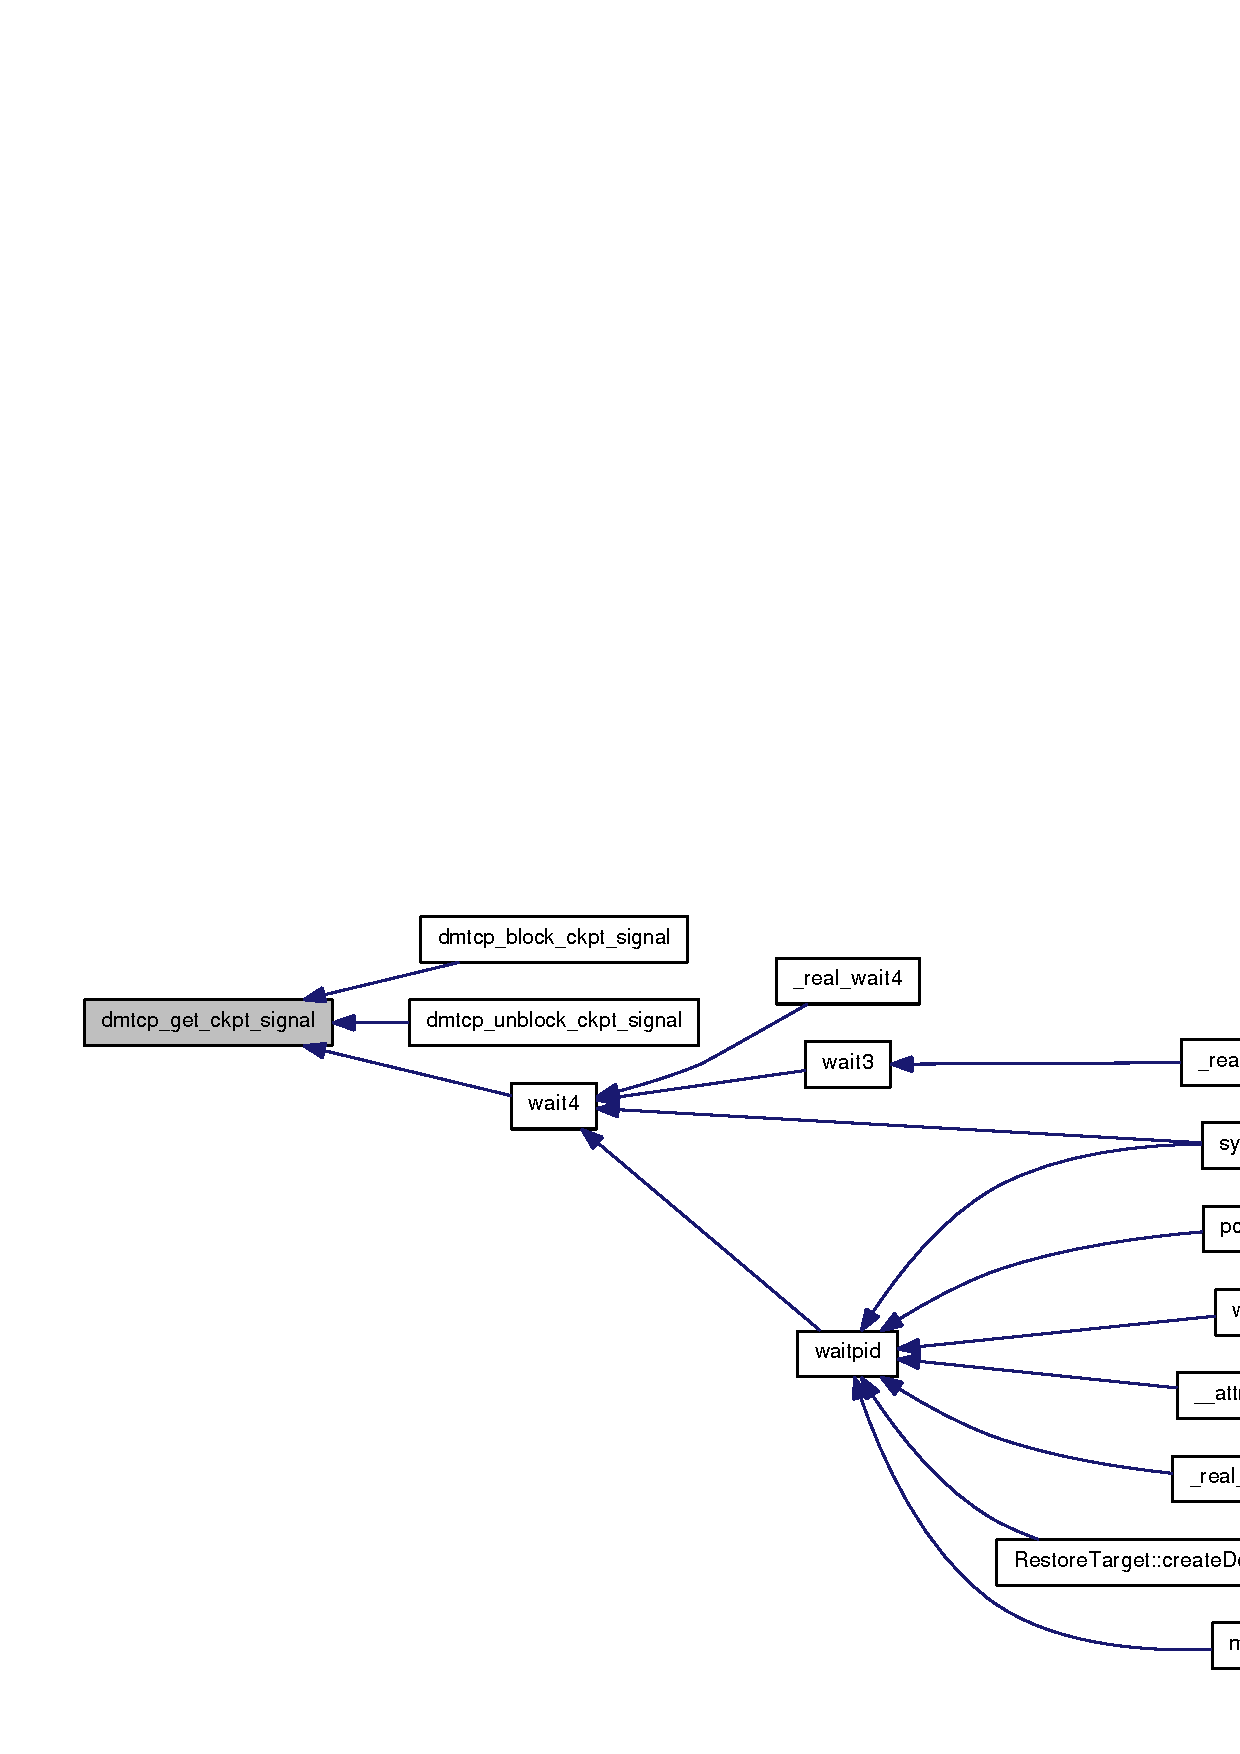
\includegraphics[width=420pt]{dmtcpinterface_8h_a586917e27ae1ef796f9a1d3632f1fc84_icgraph}
\end{center}
\end{figure}
\hypertarget{dmtcpinterface_8h_a566b789c5968c2e760171ac01dbb6d91}{
\index{dmtcpinterface.h@{dmtcpinterface.h}!dmtcp\_\-get\_\-tmpdir@{dmtcp\_\-get\_\-tmpdir}}
\index{dmtcp\_\-get\_\-tmpdir@{dmtcp\_\-get\_\-tmpdir}!dmtcpinterface.h@{dmtcpinterface.h}}
\subsubsection[{dmtcp\_\-get\_\-tmpdir}]{\setlength{\rightskip}{0pt plus 5cm}const char$\ast$ dmtcp\_\-get\_\-tmpdir ()}}
\label{dmtcpinterface_8h_a566b789c5968c2e760171ac01dbb6d91}


呼出しグラフ:\nopagebreak
\begin{figure}[H]
\begin{center}
\leavevmode
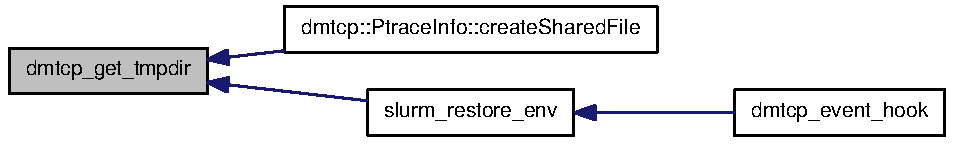
\includegraphics[width=247pt]{dmtcpinterface_8h_a566b789c5968c2e760171ac01dbb6d91_icgraph}
\end{center}
\end{figure}
\hypertarget{dmtcpinterface_8h_ad66efb25452c3dc520dc0aef3b126543}{
\index{dmtcpinterface.h@{dmtcpinterface.h}!dmtcp\_\-get\_\-uniquepid\_\-str@{dmtcp\_\-get\_\-uniquepid\_\-str}}
\index{dmtcp\_\-get\_\-uniquepid\_\-str@{dmtcp\_\-get\_\-uniquepid\_\-str}!dmtcpinterface.h@{dmtcpinterface.h}}
\subsubsection[{dmtcp\_\-get\_\-uniquepid\_\-str}]{\setlength{\rightskip}{0pt plus 5cm}const char$\ast$ dmtcp\_\-get\_\-uniquepid\_\-str ()}}
\label{dmtcpinterface_8h_ad66efb25452c3dc520dc0aef3b126543}


関数の呼び出しグラフ:\nopagebreak
\begin{figure}[H]
\begin{center}
\leavevmode
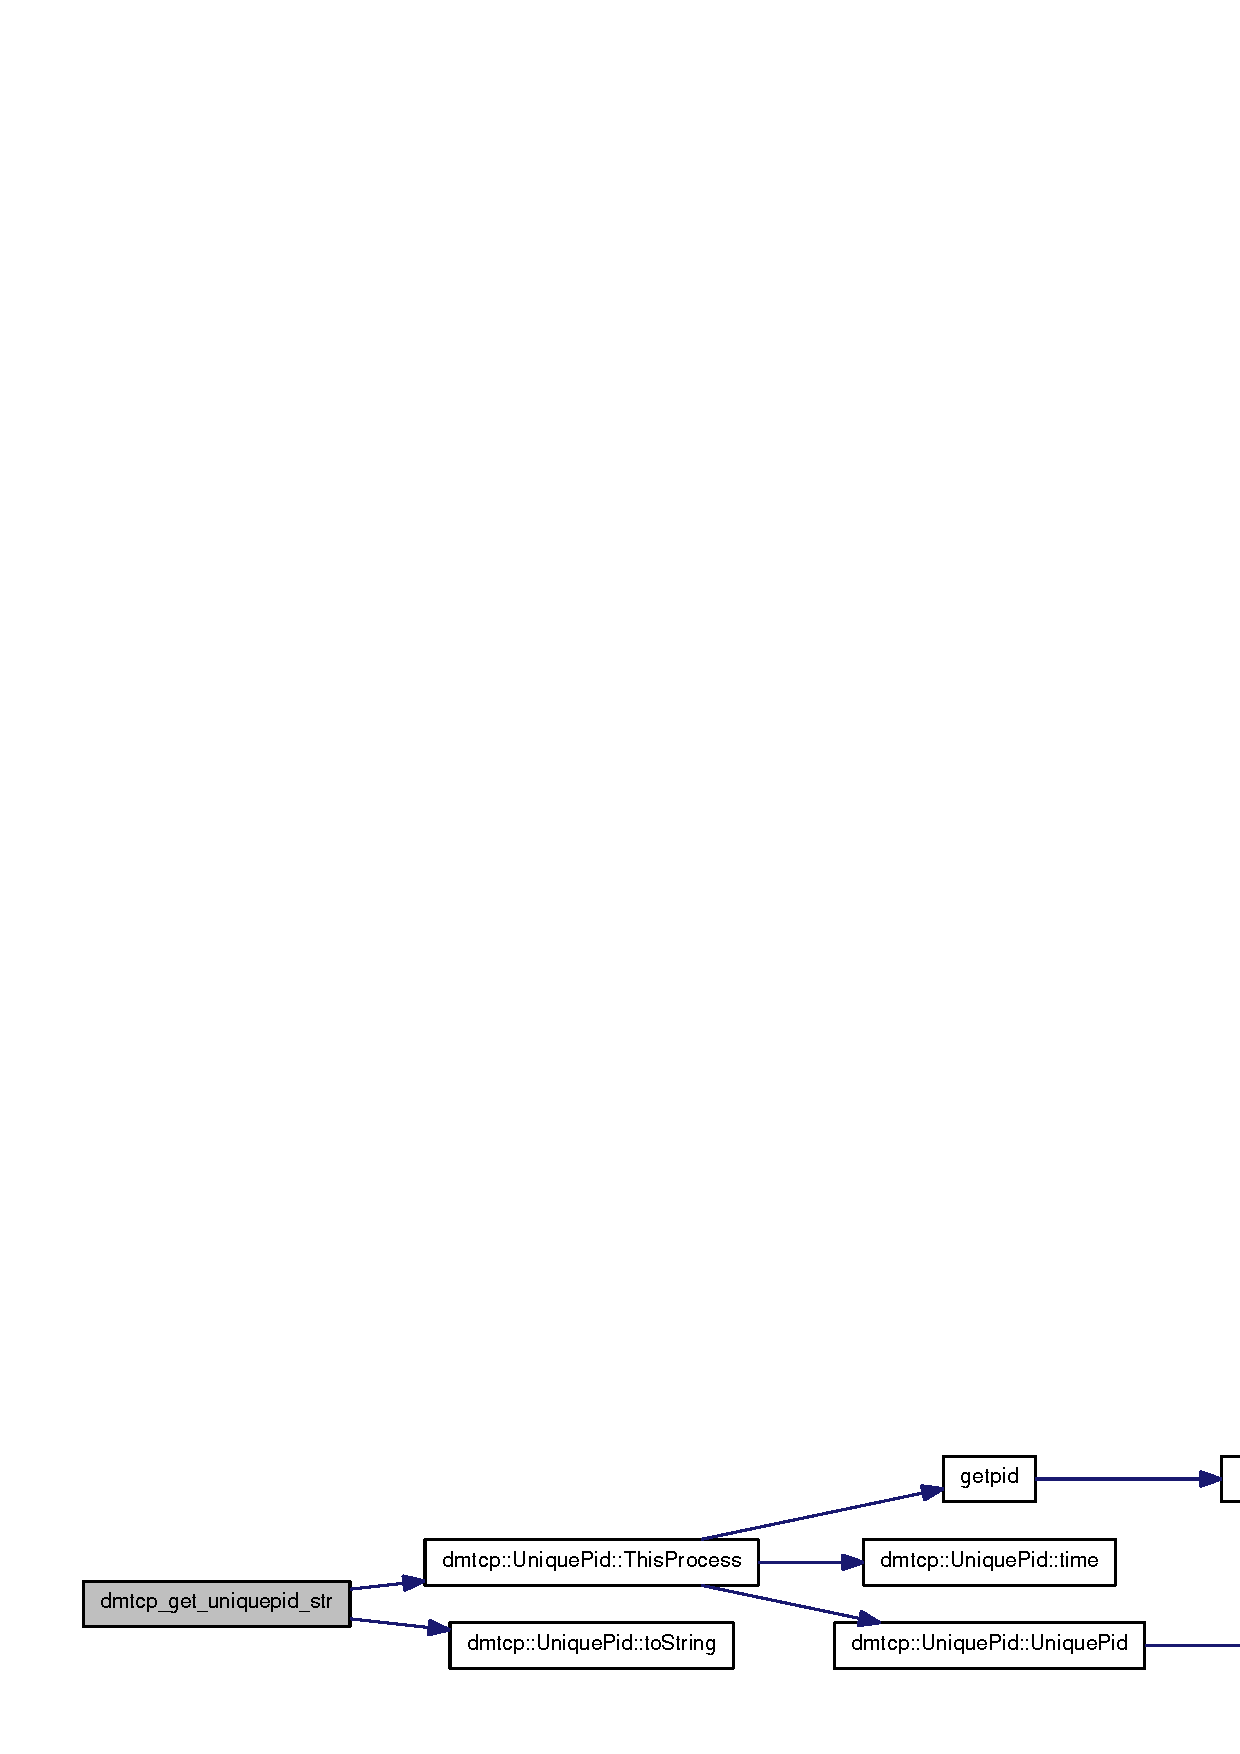
\includegraphics[width=420pt]{dmtcpinterface_8h_ad66efb25452c3dc520dc0aef3b126543_cgraph}
\end{center}
\end{figure}
\hypertarget{dmtcpinterface_8h_a63b295126a98768b49e59652a5856031}{
\index{dmtcpinterface.h@{dmtcpinterface.h}!dmtcp\_\-is\_\-running\_\-state@{dmtcp\_\-is\_\-running\_\-state}}
\index{dmtcp\_\-is\_\-running\_\-state@{dmtcp\_\-is\_\-running\_\-state}!dmtcpinterface.h@{dmtcpinterface.h}}
\subsubsection[{dmtcp\_\-is\_\-running\_\-state}]{\setlength{\rightskip}{0pt plus 5cm}int dmtcp\_\-is\_\-running\_\-state ()}}
\label{dmtcpinterface_8h_a63b295126a98768b49e59652a5856031}


呼出しグラフ:\nopagebreak
\begin{figure}[H]
\begin{center}
\leavevmode
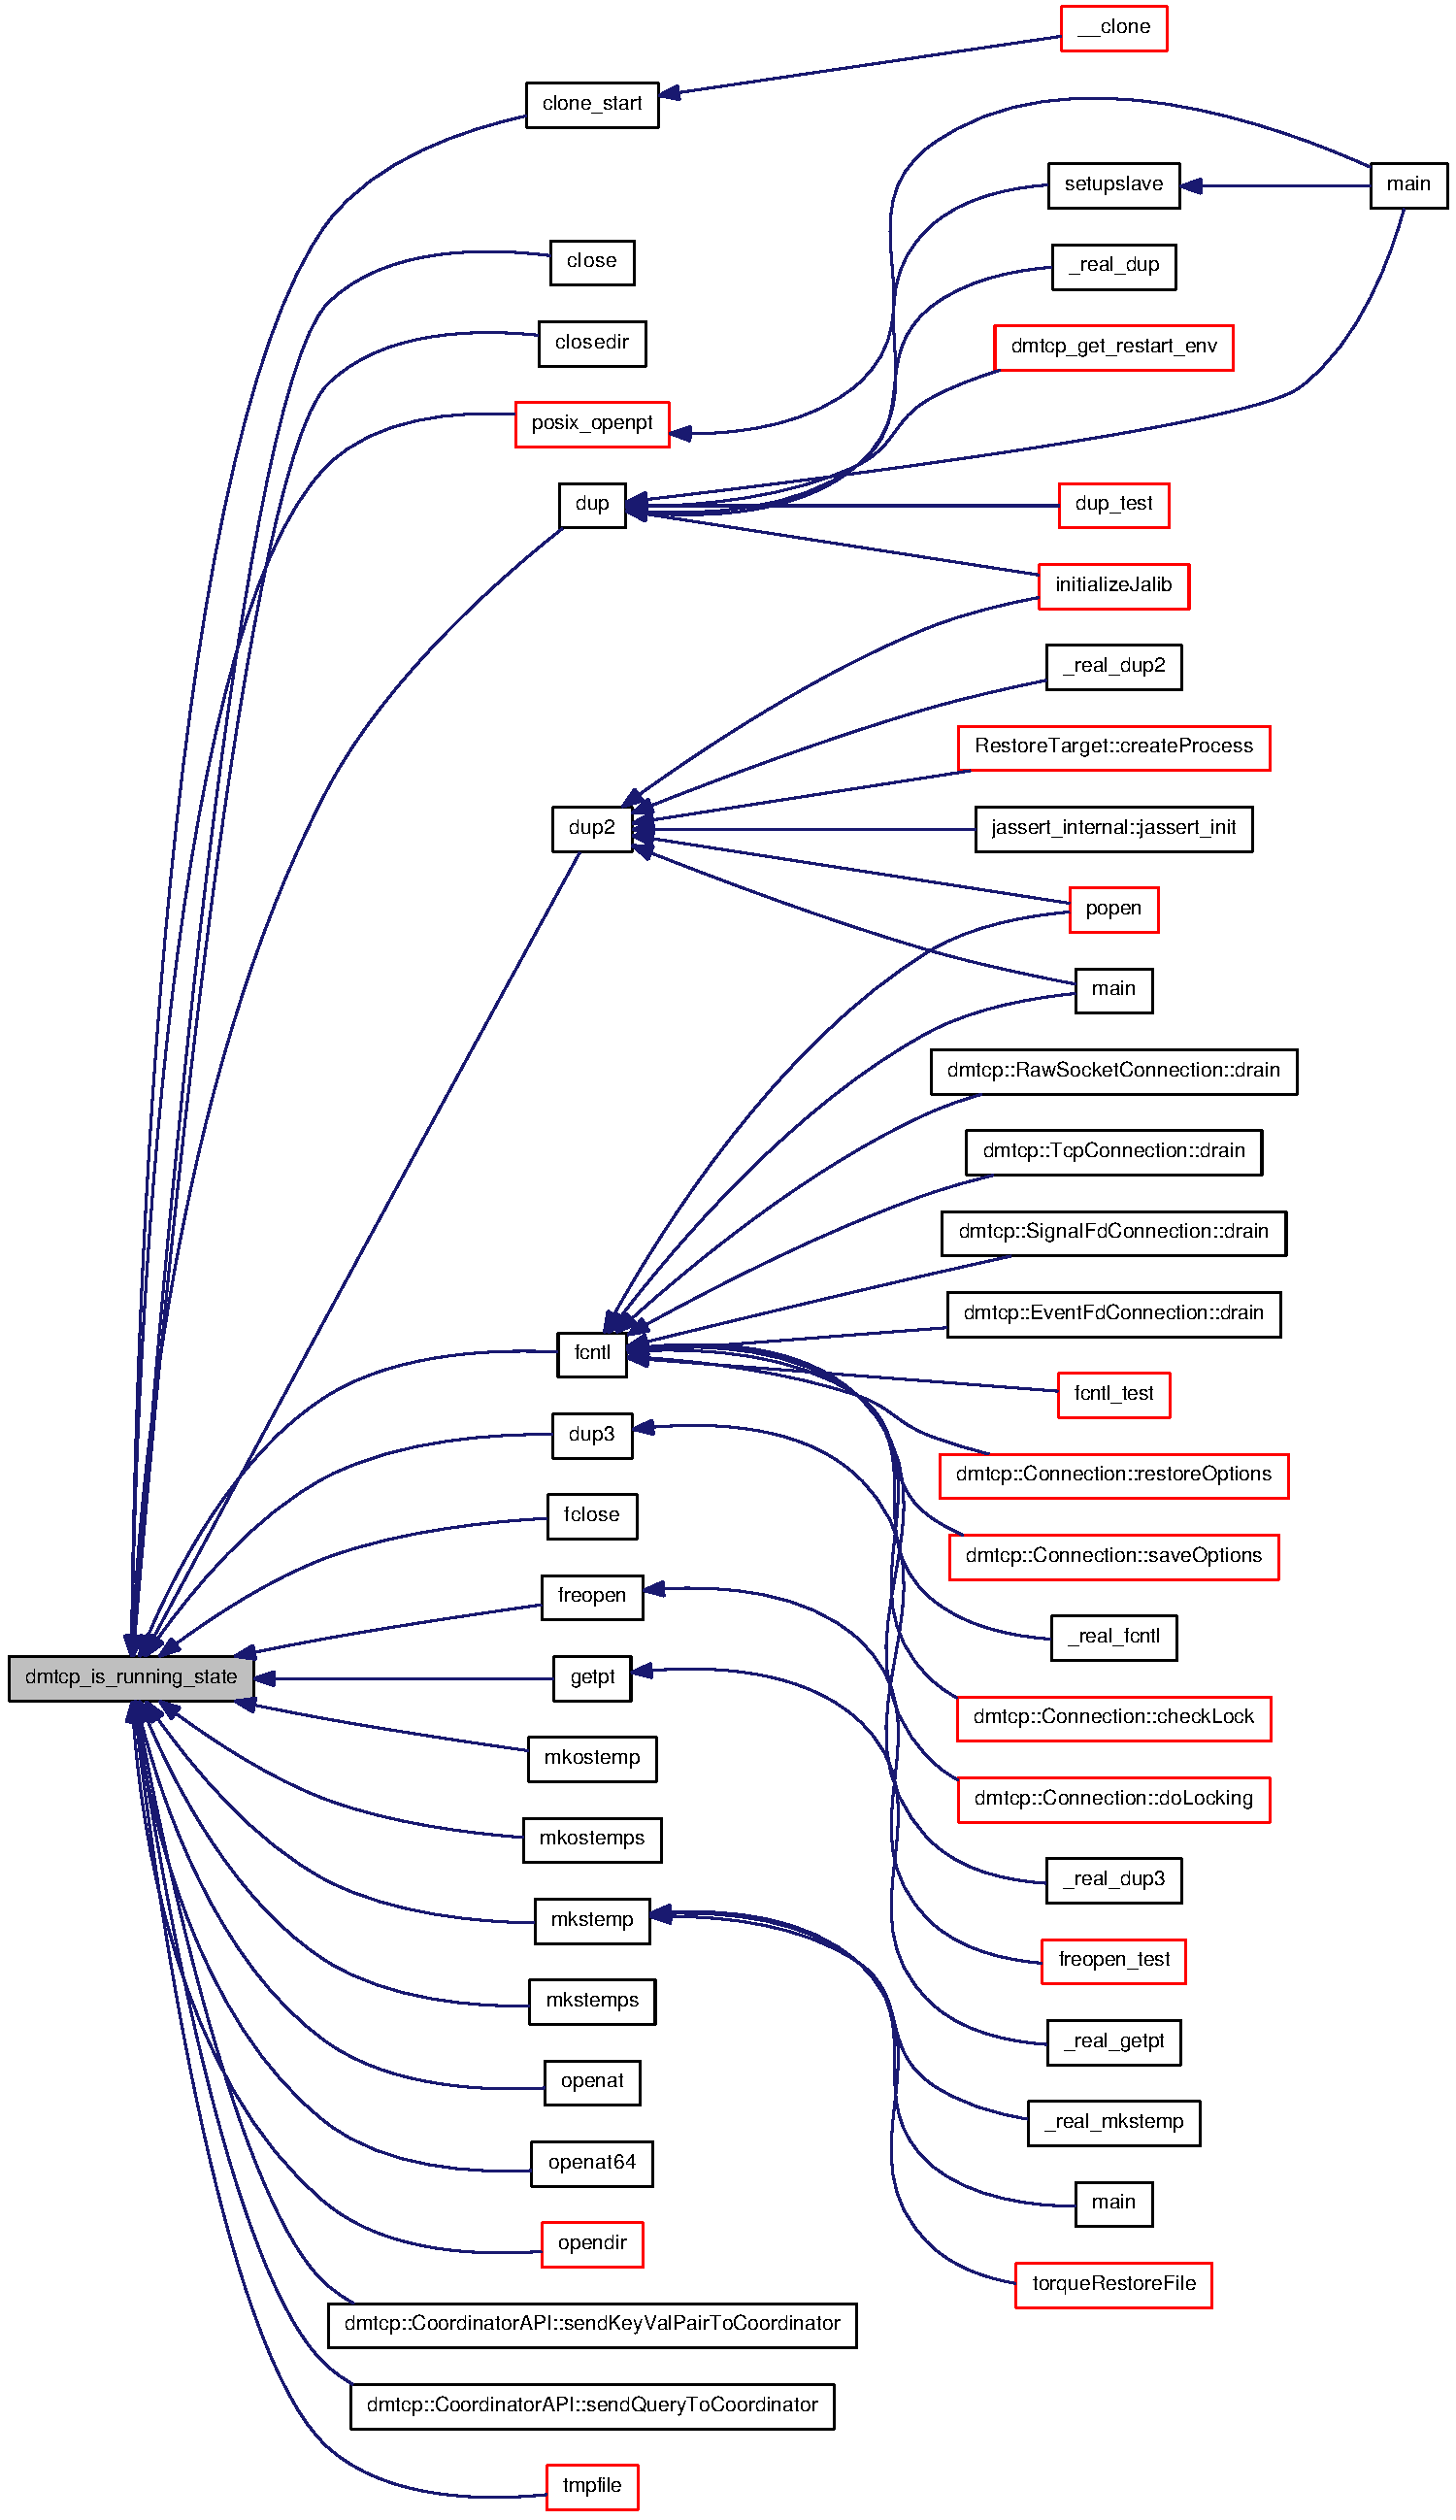
\includegraphics[width=378pt]{dmtcpinterface_8h_a63b295126a98768b49e59652a5856031_icgraph}
\end{center}
\end{figure}
\hypertarget{dmtcpinterface_8h_ab84d885ac90fd3a2490f353906df9548}{
\index{dmtcpinterface.h@{dmtcpinterface.h}!process\_\-dmtcp\_\-event@{process\_\-dmtcp\_\-event}}
\index{process\_\-dmtcp\_\-event@{process\_\-dmtcp\_\-event}!dmtcpinterface.h@{dmtcpinterface.h}}
\subsubsection[{process\_\-dmtcp\_\-event}]{\setlength{\rightskip}{0pt plus 5cm}void process\_\-dmtcp\_\-event ({\bf DmtcpEvent\_\-t} {\em event}, \/  void $\ast$ {\em data})}}
\label{dmtcpinterface_8h_ab84d885ac90fd3a2490f353906df9548}

\hypertarget{artem__rc__pingpong_8c}{
\section{contrib/infiniband/examples/artem\_\-rc\_\-pingpong.c}
\label{artem__rc__pingpong_8c}\index{contrib/infiniband/examples/artem\_\-rc\_\-pingpong.c@{contrib/infiniband/examples/artem\_\-rc\_\-pingpong.c}}
}
{\ttfamily \#include $<$stdio.h$>$}\par
{\ttfamily \#include $<$stdlib.h$>$}\par
{\ttfamily \#include $<$unistd.h$>$}\par
{\ttfamily \#include $<$string.h$>$}\par
{\ttfamily \#include $<$sys/types.h$>$}\par
{\ttfamily \#include $<$sys/socket.h$>$}\par
{\ttfamily \#include $<$sys/time.h$>$}\par
{\ttfamily \#include $<$netdb.h$>$}\par
{\ttfamily \#include $<$malloc.h$>$}\par
{\ttfamily \#include $<$getopt.h$>$}\par
{\ttfamily \#include $<$arpa/inet.h$>$}\par
{\ttfamily \#include $<$time.h$>$}\par
{\ttfamily \#include \char`\"{}pingpong.h\char`\"{}}\par
artem\_\-rc\_\-pingpong.cのインクルード依存関係図\nopagebreak
\begin{figure}[H]
\begin{center}
\leavevmode
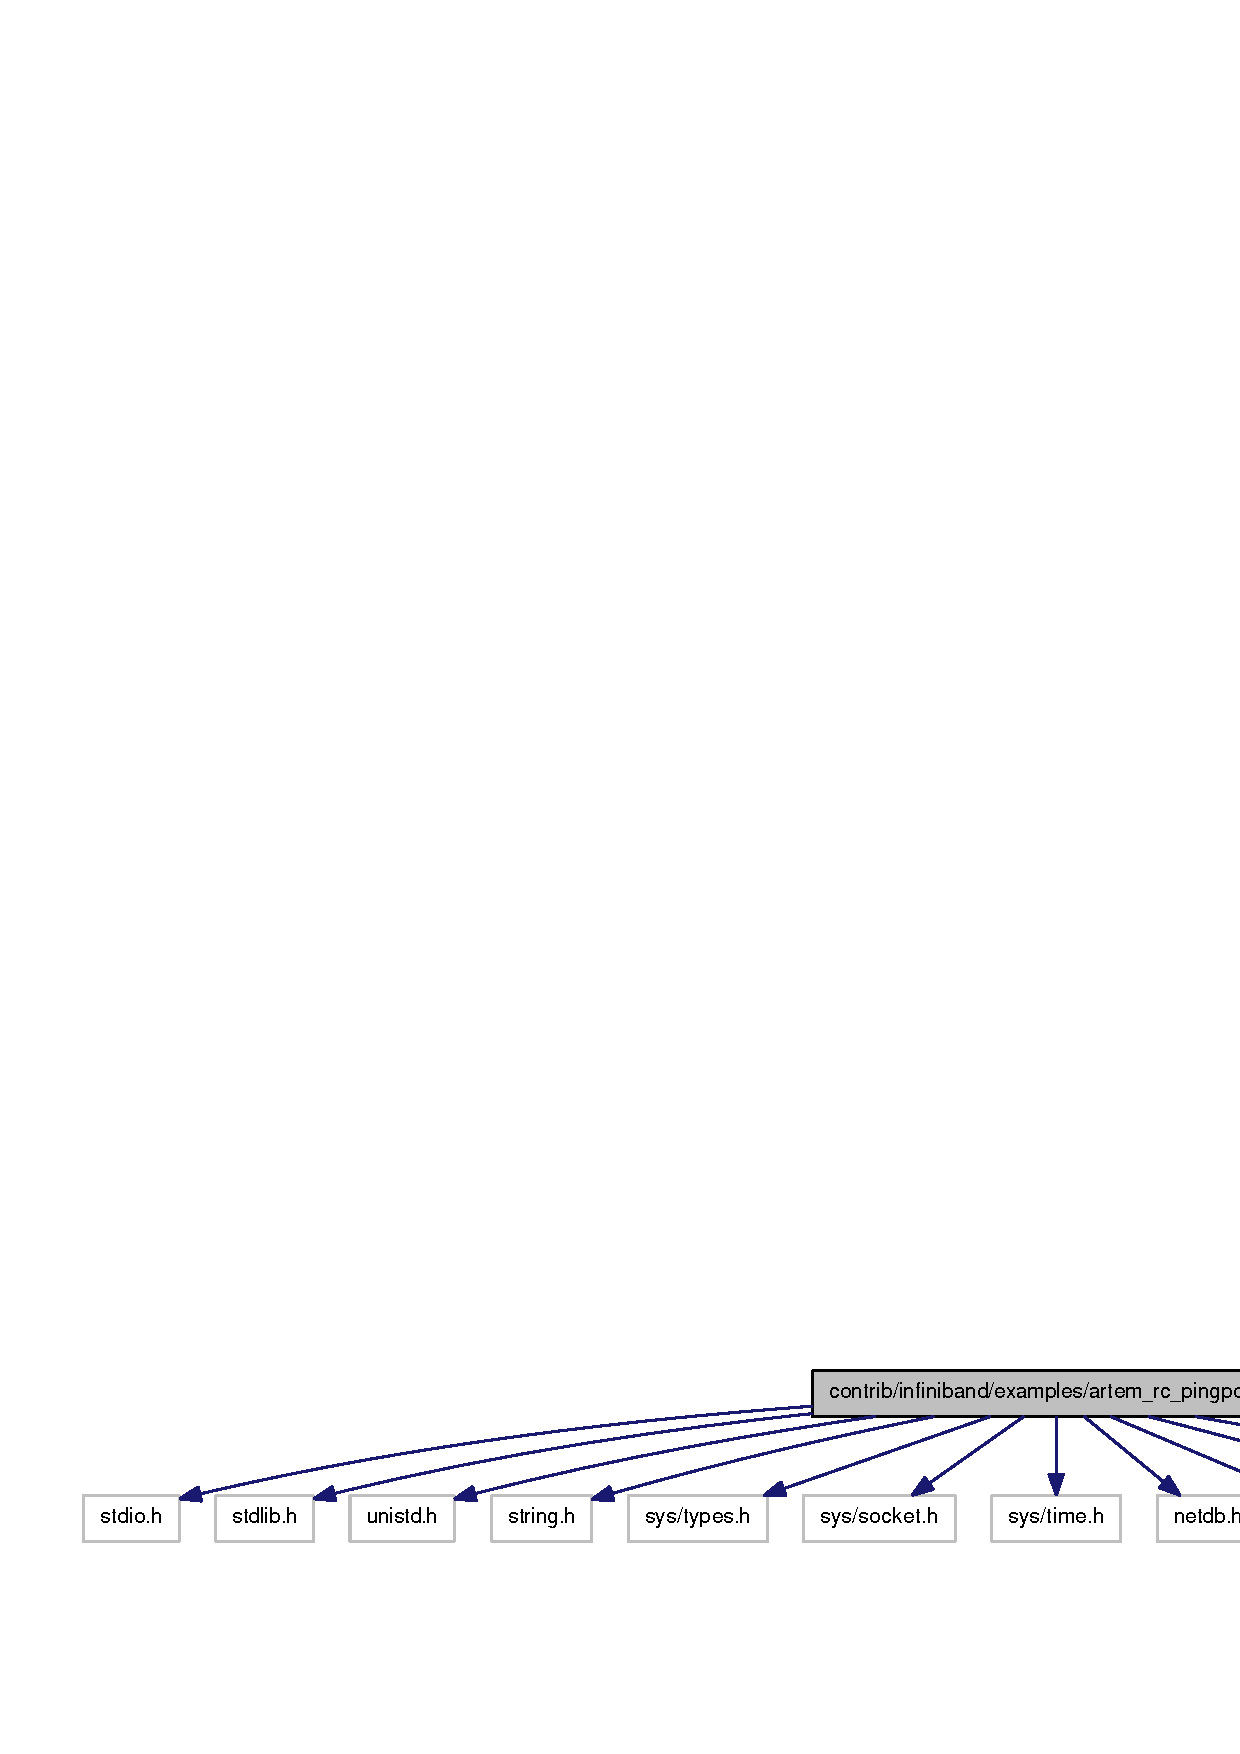
\includegraphics[width=420pt]{artem__rc__pingpong_8c__incl}
\end{center}
\end{figure}
\subsection*{構成}
\begin{DoxyCompactItemize}
\item 
struct \hyperlink{structbuffer}{buffer}
\item 
struct \hyperlink{structpcontext}{pcontext}
\item 
struct \hyperlink{structpdest}{pdest}
\end{DoxyCompactItemize}
\subsection*{マクロ定義}
\begin{DoxyCompactItemize}
\item 
\#define \hyperlink{artem__rc__pingpong_8c_a5a9cc968ee7262fddda93f73341beedb}{PDEBUG}(fmt, args...)~printf(fmt\char`\"{}$\backslash$n\char`\"{}, \#\#args );
\item 
\#define \hyperlink{artem__rc__pingpong_8c_a403cf3149c084cea115b85c90721039a}{BSIZE}~256
\end{DoxyCompactItemize}
\subsection*{型定義}
\begin{DoxyCompactItemize}
\item 
typedef unsigned int \hyperlink{artem__rc__pingpong_8c_a91ad9478d81a7aaf2593e8d9c3d06a14}{uint}
\end{DoxyCompactItemize}
\subsection*{列挙型}
\begin{DoxyCompactItemize}
\item 
enum \{ \hyperlink{artem__rc__pingpong_8c_a06fc87d81c62e9abb8790b6e5713c55ba40a98b3dc4da4afaad19e4b24bab3d4b}{PINGPONG\_\-RECV\_\-WRID} =  1, 
\hyperlink{artem__rc__pingpong_8c_a06fc87d81c62e9abb8790b6e5713c55ba808d047a9dae56ee90046924355b6069}{PINGPONG\_\-SEND\_\-WRID} =  2
 \}
\end{DoxyCompactItemize}
\subsection*{関数}
\begin{DoxyCompactItemize}
\item 
\hyperlink{artem__rc__pingpong_8c_a91ad9478d81a7aaf2593e8d9c3d06a14}{uint} \hyperlink{artem__rc__pingpong_8c_a618f0b791ad7905aca1be71cdd3e17b7}{buf\_\-inc} (\hyperlink{artem__rc__pingpong_8c_a91ad9478d81a7aaf2593e8d9c3d06a14}{uint} c, \hyperlink{artem__rc__pingpong_8c_a91ad9478d81a7aaf2593e8d9c3d06a14}{uint} modulo)
\item 
int \hyperlink{artem__rc__pingpong_8c_a5f4d21f4eaa1361b1a7b844fa7f4af94}{buf\_\-add} (struct \hyperlink{structbuffer}{buffer} $\ast$b)
\item 
int \hyperlink{artem__rc__pingpong_8c_a53c1d629466d88bc87055cd2efa52335}{buf\_\-del} (struct \hyperlink{structbuffer}{buffer} $\ast$b)
\item 
unsigned int \hyperlink{artem__rc__pingpong_8c_ac81621b9bd04e17b6eb4bcd80f78fcdd}{buf\_\-free} (struct \hyperlink{structbuffer}{buffer} $\ast$b)
\item 
\hyperlink{artem__rc__pingpong_8c_a91ad9478d81a7aaf2593e8d9c3d06a14}{uint} \hyperlink{artem__rc__pingpong_8c_a58b5a10b205f160534641abd5b7792dd}{buf\_\-used} (struct \hyperlink{structbuffer}{buffer} $\ast$b)
\item 
int \hyperlink{artem__rc__pingpong_8c_a7a76c3673a201262ddad0e6b4e7dab9c}{close\_\-ctx} (struct \hyperlink{structpcontext}{pcontext} $\ast$ctx)
\item 
int \hyperlink{artem__rc__pingpong_8c_a0ddf1224851353fc92bfbff6f499fa97}{main} (int argc, char $\ast$argv\mbox{[}$\,$\mbox{]})
\end{DoxyCompactItemize}
\subsection*{変数}
\begin{DoxyCompactItemize}
\item 
\hyperlink{artem__rc__pingpong_8c_a91ad9478d81a7aaf2593e8d9c3d06a14}{uint} \hyperlink{artem__rc__pingpong_8c_abab635a378d9ff76cbc0b91e997081e4}{rem\_\-unack\_\-tot} = 0
\item 
\hyperlink{artem__rc__pingpong_8c_a91ad9478d81a7aaf2593e8d9c3d06a14}{uint} \hyperlink{artem__rc__pingpong_8c_ad06efed141aae735dde3d59c3cf93890}{rem\_\-unack\_\-count} = 0
\item 
\hyperlink{artem__rc__pingpong_8c_a91ad9478d81a7aaf2593e8d9c3d06a14}{uint} \hyperlink{artem__rc__pingpong_8c_a7f508a72aa28dbdbfa0dc82d191c0983}{local\_\-unack\_\-tot} = 0
\item 
\hyperlink{artem__rc__pingpong_8c_a91ad9478d81a7aaf2593e8d9c3d06a14}{uint} \hyperlink{artem__rc__pingpong_8c_ac070153ead1986a5f0bed7b57ded8888}{local\_\-unack\_\-count} = 0
\end{DoxyCompactItemize}


\subsection{マクロ定義}
\hypertarget{artem__rc__pingpong_8c_a403cf3149c084cea115b85c90721039a}{
\index{artem\_\-rc\_\-pingpong.c@{artem\_\-rc\_\-pingpong.c}!BSIZE@{BSIZE}}
\index{BSIZE@{BSIZE}!artem_rc_pingpong.c@{artem\_\-rc\_\-pingpong.c}}
\subsubsection[{BSIZE}]{\setlength{\rightskip}{0pt plus 5cm}\#define BSIZE~256}}
\label{artem__rc__pingpong_8c_a403cf3149c084cea115b85c90721039a}
\hypertarget{artem__rc__pingpong_8c_a5a9cc968ee7262fddda93f73341beedb}{
\index{artem\_\-rc\_\-pingpong.c@{artem\_\-rc\_\-pingpong.c}!PDEBUG@{PDEBUG}}
\index{PDEBUG@{PDEBUG}!artem_rc_pingpong.c@{artem\_\-rc\_\-pingpong.c}}
\subsubsection[{PDEBUG}]{\setlength{\rightskip}{0pt plus 5cm}\#define PDEBUG(fmt, \/  args...)~printf(fmt\char`\"{}$\backslash$n\char`\"{}, \#\#args );}}
\label{artem__rc__pingpong_8c_a5a9cc968ee7262fddda93f73341beedb}


\subsection{型定義}
\hypertarget{artem__rc__pingpong_8c_a91ad9478d81a7aaf2593e8d9c3d06a14}{
\index{artem\_\-rc\_\-pingpong.c@{artem\_\-rc\_\-pingpong.c}!uint@{uint}}
\index{uint@{uint}!artem_rc_pingpong.c@{artem\_\-rc\_\-pingpong.c}}
\subsubsection[{uint}]{\setlength{\rightskip}{0pt plus 5cm}typedef unsigned int {\bf uint}}}
\label{artem__rc__pingpong_8c_a91ad9478d81a7aaf2593e8d9c3d06a14}


\subsection{列挙型}
\hypertarget{artem__rc__pingpong_8c_a06fc87d81c62e9abb8790b6e5713c55b}{
\subsubsection[{"@0}]{\setlength{\rightskip}{0pt plus 5cm}anonymous enum}}
\label{artem__rc__pingpong_8c_a06fc87d81c62e9abb8790b6e5713c55b}
\begin{Desc}
\item[列挙型の値: ]\par
\begin{description}
\index{PINGPONG\_\-RECV\_\-WRID@{PINGPONG\_\-RECV\_\-WRID}!artem\_\-rc\_\-pingpong.c@{artem\_\-rc\_\-pingpong.c}}\index{artem\_\-rc\_\-pingpong.c@{artem\_\-rc\_\-pingpong.c}!PINGPONG\_\-RECV\_\-WRID@{PINGPONG\_\-RECV\_\-WRID}}\item[{\em 
\hypertarget{artem__rc__pingpong_8c_a06fc87d81c62e9abb8790b6e5713c55ba40a98b3dc4da4afaad19e4b24bab3d4b}{
PINGPONG\_\-RECV\_\-WRID}
\label{artem__rc__pingpong_8c_a06fc87d81c62e9abb8790b6e5713c55ba40a98b3dc4da4afaad19e4b24bab3d4b}
}]\index{PINGPONG\_\-SEND\_\-WRID@{PINGPONG\_\-SEND\_\-WRID}!artem\_\-rc\_\-pingpong.c@{artem\_\-rc\_\-pingpong.c}}\index{artem\_\-rc\_\-pingpong.c@{artem\_\-rc\_\-pingpong.c}!PINGPONG\_\-SEND\_\-WRID@{PINGPONG\_\-SEND\_\-WRID}}\item[{\em 
\hypertarget{artem__rc__pingpong_8c_a06fc87d81c62e9abb8790b6e5713c55ba808d047a9dae56ee90046924355b6069}{
PINGPONG\_\-SEND\_\-WRID}
\label{artem__rc__pingpong_8c_a06fc87d81c62e9abb8790b6e5713c55ba808d047a9dae56ee90046924355b6069}
}]\end{description}
\end{Desc}



\subsection{関数}
\hypertarget{artem__rc__pingpong_8c_a5f4d21f4eaa1361b1a7b844fa7f4af94}{
\index{artem\_\-rc\_\-pingpong.c@{artem\_\-rc\_\-pingpong.c}!buf\_\-add@{buf\_\-add}}
\index{buf\_\-add@{buf\_\-add}!artem_rc_pingpong.c@{artem\_\-rc\_\-pingpong.c}}
\subsubsection[{buf\_\-add}]{\setlength{\rightskip}{0pt plus 5cm}int buf\_\-add (struct {\bf buffer} $\ast$ {\em b})\hspace{0.3cm}{\ttfamily  \mbox{[}inline\mbox{]}}}}
\label{artem__rc__pingpong_8c_a5f4d21f4eaa1361b1a7b844fa7f4af94}


関数の呼び出しグラフ:\nopagebreak
\begin{figure}[H]
\begin{center}
\leavevmode
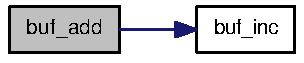
\includegraphics[width=91pt]{artem__rc__pingpong_8c_a5f4d21f4eaa1361b1a7b844fa7f4af94_cgraph}
\end{center}
\end{figure}
\hypertarget{artem__rc__pingpong_8c_a53c1d629466d88bc87055cd2efa52335}{
\index{artem\_\-rc\_\-pingpong.c@{artem\_\-rc\_\-pingpong.c}!buf\_\-del@{buf\_\-del}}
\index{buf\_\-del@{buf\_\-del}!artem_rc_pingpong.c@{artem\_\-rc\_\-pingpong.c}}
\subsubsection[{buf\_\-del}]{\setlength{\rightskip}{0pt plus 5cm}int buf\_\-del (struct {\bf buffer} $\ast$ {\em b})\hspace{0.3cm}{\ttfamily  \mbox{[}inline\mbox{]}}}}
\label{artem__rc__pingpong_8c_a53c1d629466d88bc87055cd2efa52335}


関数の呼び出しグラフ:\nopagebreak
\begin{figure}[H]
\begin{center}
\leavevmode
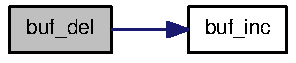
\includegraphics[width=89pt]{artem__rc__pingpong_8c_a53c1d629466d88bc87055cd2efa52335_cgraph}
\end{center}
\end{figure}


呼出しグラフ:\nopagebreak
\begin{figure}[H]
\begin{center}
\leavevmode
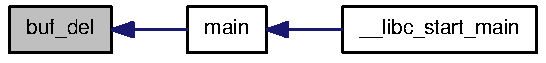
\includegraphics[width=149pt]{artem__rc__pingpong_8c_a53c1d629466d88bc87055cd2efa52335_icgraph}
\end{center}
\end{figure}
\hypertarget{artem__rc__pingpong_8c_ac81621b9bd04e17b6eb4bcd80f78fcdd}{
\index{artem\_\-rc\_\-pingpong.c@{artem\_\-rc\_\-pingpong.c}!buf\_\-free@{buf\_\-free}}
\index{buf\_\-free@{buf\_\-free}!artem_rc_pingpong.c@{artem\_\-rc\_\-pingpong.c}}
\subsubsection[{buf\_\-free}]{\setlength{\rightskip}{0pt plus 5cm}unsigned int buf\_\-free (struct {\bf buffer} $\ast$ {\em b})\hspace{0.3cm}{\ttfamily  \mbox{[}inline\mbox{]}}}}
\label{artem__rc__pingpong_8c_ac81621b9bd04e17b6eb4bcd80f78fcdd}


呼出しグラフ:\nopagebreak
\begin{figure}[H]
\begin{center}
\leavevmode
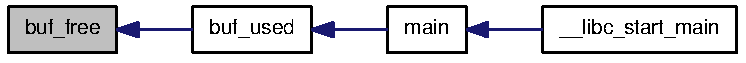
\includegraphics[width=197pt]{artem__rc__pingpong_8c_ac81621b9bd04e17b6eb4bcd80f78fcdd_icgraph}
\end{center}
\end{figure}
\hypertarget{artem__rc__pingpong_8c_a618f0b791ad7905aca1be71cdd3e17b7}{
\index{artem\_\-rc\_\-pingpong.c@{artem\_\-rc\_\-pingpong.c}!buf\_\-inc@{buf\_\-inc}}
\index{buf\_\-inc@{buf\_\-inc}!artem_rc_pingpong.c@{artem\_\-rc\_\-pingpong.c}}
\subsubsection[{buf\_\-inc}]{\setlength{\rightskip}{0pt plus 5cm}{\bf uint} buf\_\-inc ({\bf uint} {\em c}, \/  {\bf uint} {\em modulo})\hspace{0.3cm}{\ttfamily  \mbox{[}inline\mbox{]}}}}
\label{artem__rc__pingpong_8c_a618f0b791ad7905aca1be71cdd3e17b7}


呼出しグラフ:\nopagebreak
\begin{figure}[H]
\begin{center}
\leavevmode
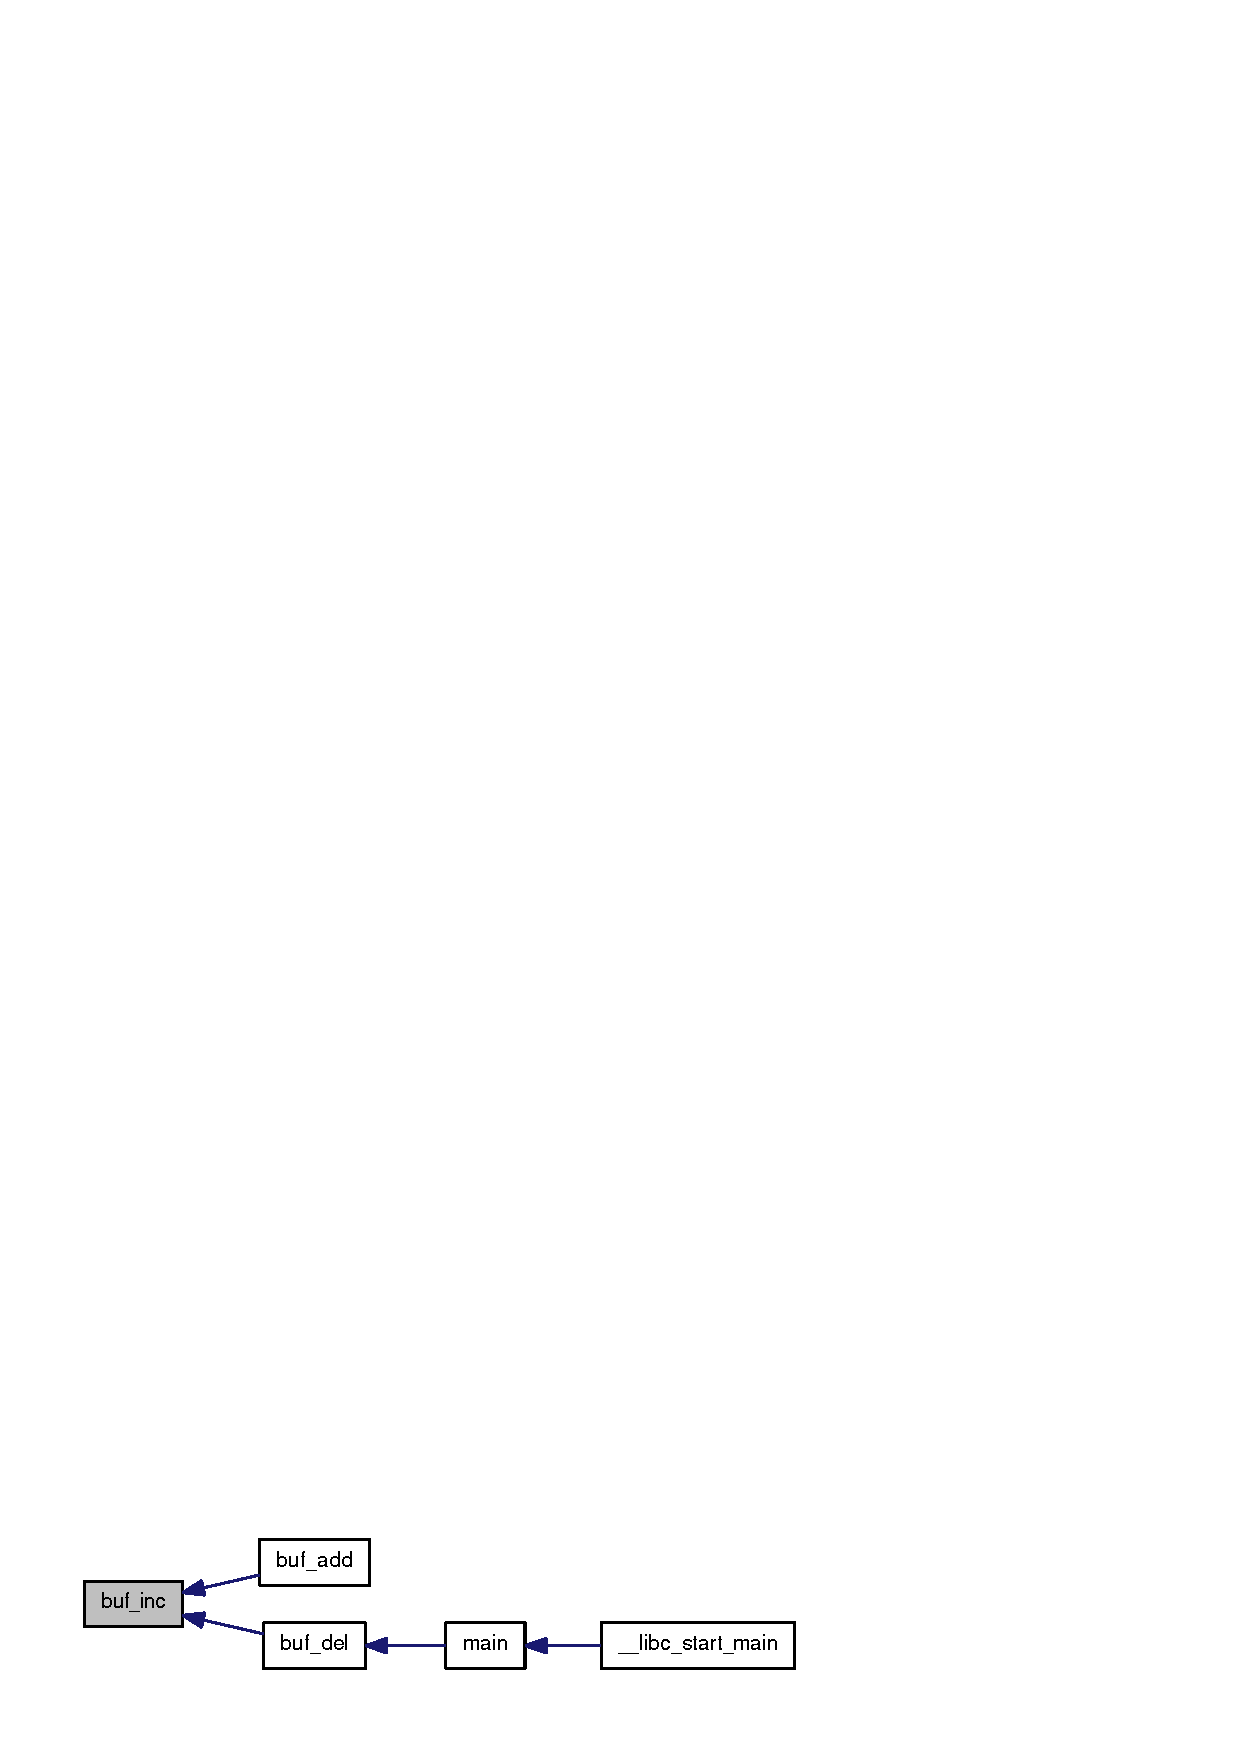
\includegraphics[width=193pt]{artem__rc__pingpong_8c_a618f0b791ad7905aca1be71cdd3e17b7_icgraph}
\end{center}
\end{figure}
\hypertarget{artem__rc__pingpong_8c_a58b5a10b205f160534641abd5b7792dd}{
\index{artem\_\-rc\_\-pingpong.c@{artem\_\-rc\_\-pingpong.c}!buf\_\-used@{buf\_\-used}}
\index{buf\_\-used@{buf\_\-used}!artem_rc_pingpong.c@{artem\_\-rc\_\-pingpong.c}}
\subsubsection[{buf\_\-used}]{\setlength{\rightskip}{0pt plus 5cm}{\bf uint} buf\_\-used (struct {\bf buffer} $\ast$ {\em b})\hspace{0.3cm}{\ttfamily  \mbox{[}inline\mbox{]}}}}
\label{artem__rc__pingpong_8c_a58b5a10b205f160534641abd5b7792dd}


関数の呼び出しグラフ:\nopagebreak
\begin{figure}[H]
\begin{center}
\leavevmode
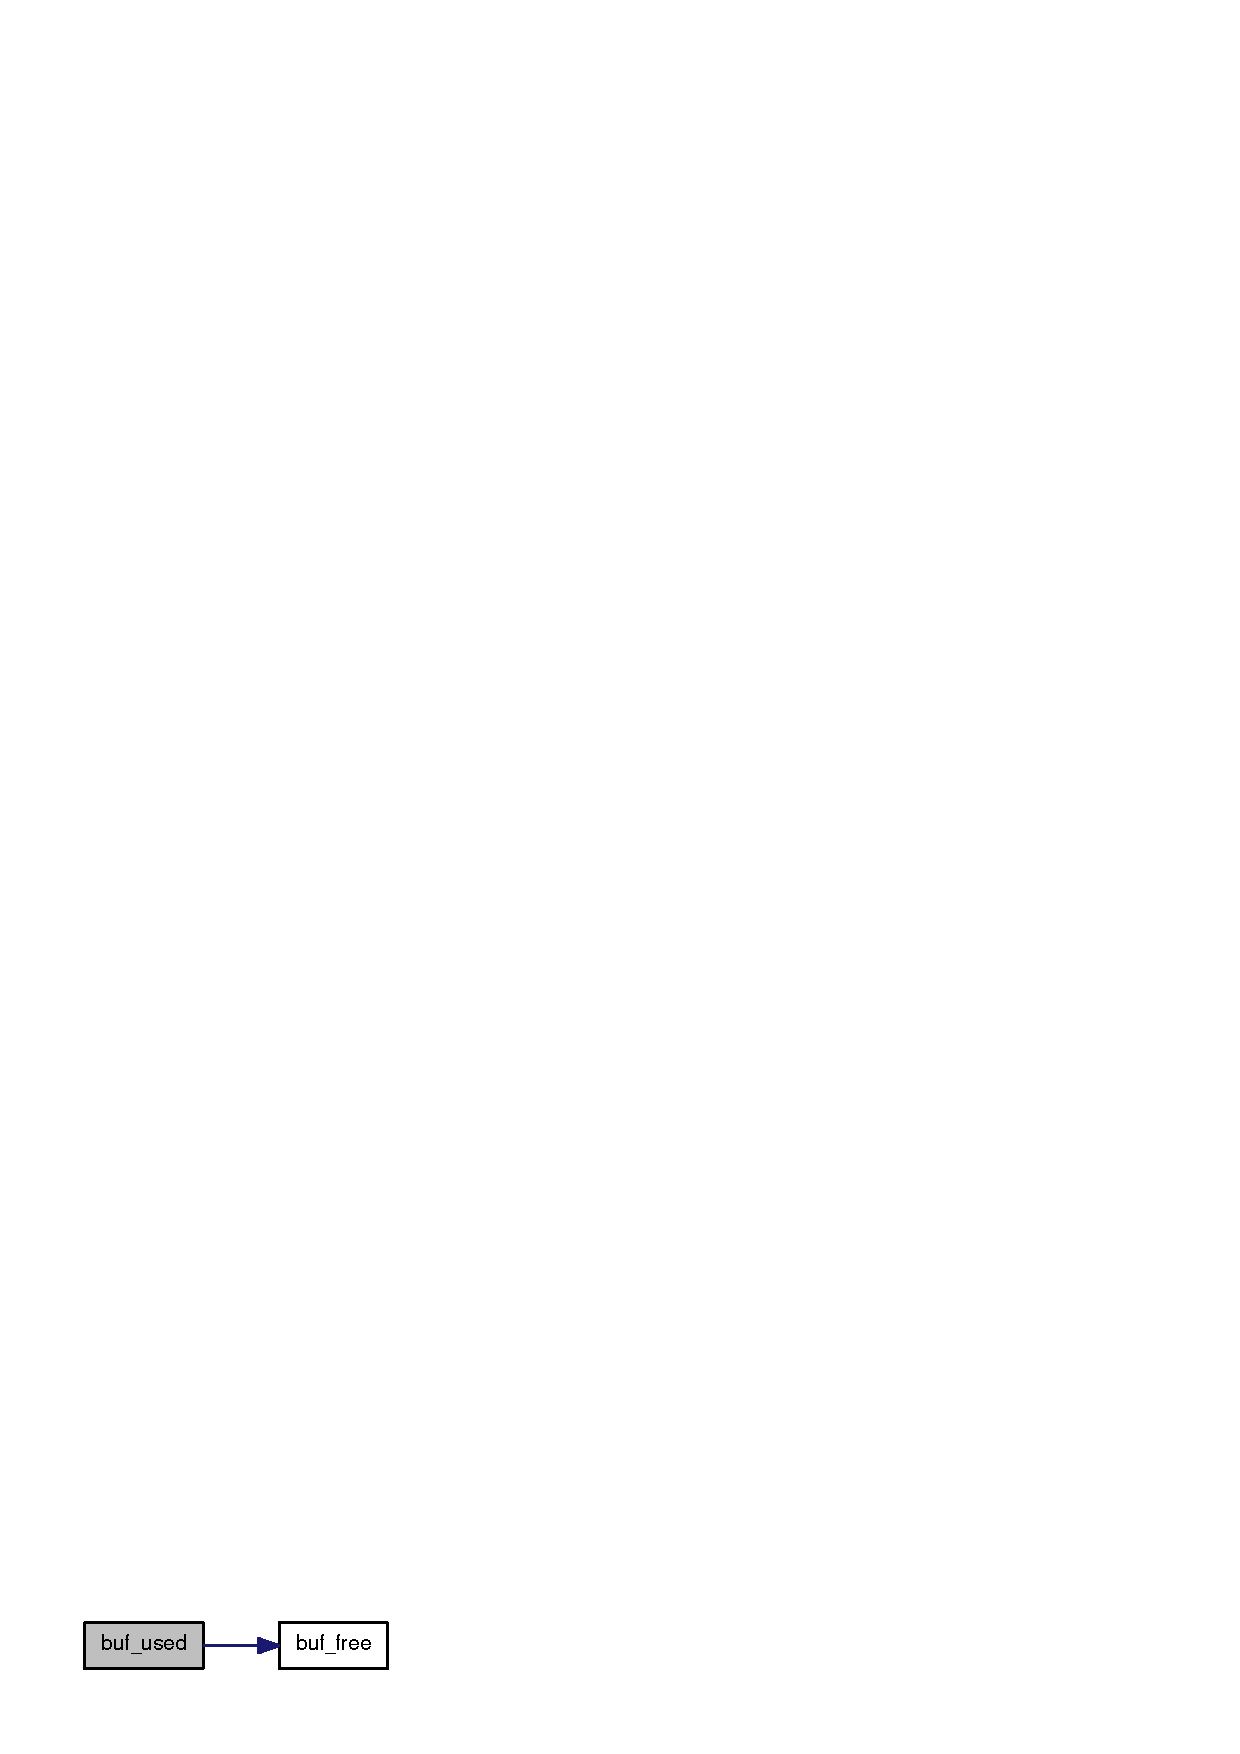
\includegraphics[width=95pt]{artem__rc__pingpong_8c_a58b5a10b205f160534641abd5b7792dd_cgraph}
\end{center}
\end{figure}


呼出しグラフ:\nopagebreak
\begin{figure}[H]
\begin{center}
\leavevmode
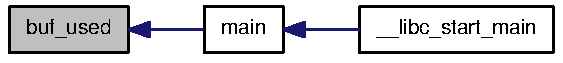
\includegraphics[width=153pt]{artem__rc__pingpong_8c_a58b5a10b205f160534641abd5b7792dd_icgraph}
\end{center}
\end{figure}
\hypertarget{artem__rc__pingpong_8c_a7a76c3673a201262ddad0e6b4e7dab9c}{
\index{artem\_\-rc\_\-pingpong.c@{artem\_\-rc\_\-pingpong.c}!close\_\-ctx@{close\_\-ctx}}
\index{close\_\-ctx@{close\_\-ctx}!artem_rc_pingpong.c@{artem\_\-rc\_\-pingpong.c}}
\subsubsection[{close\_\-ctx}]{\setlength{\rightskip}{0pt plus 5cm}int close\_\-ctx (struct {\bf pcontext} $\ast$ {\em ctx})}}
\label{artem__rc__pingpong_8c_a7a76c3673a201262ddad0e6b4e7dab9c}


関数の呼び出しグラフ:\nopagebreak
\begin{figure}[H]
\begin{center}
\leavevmode
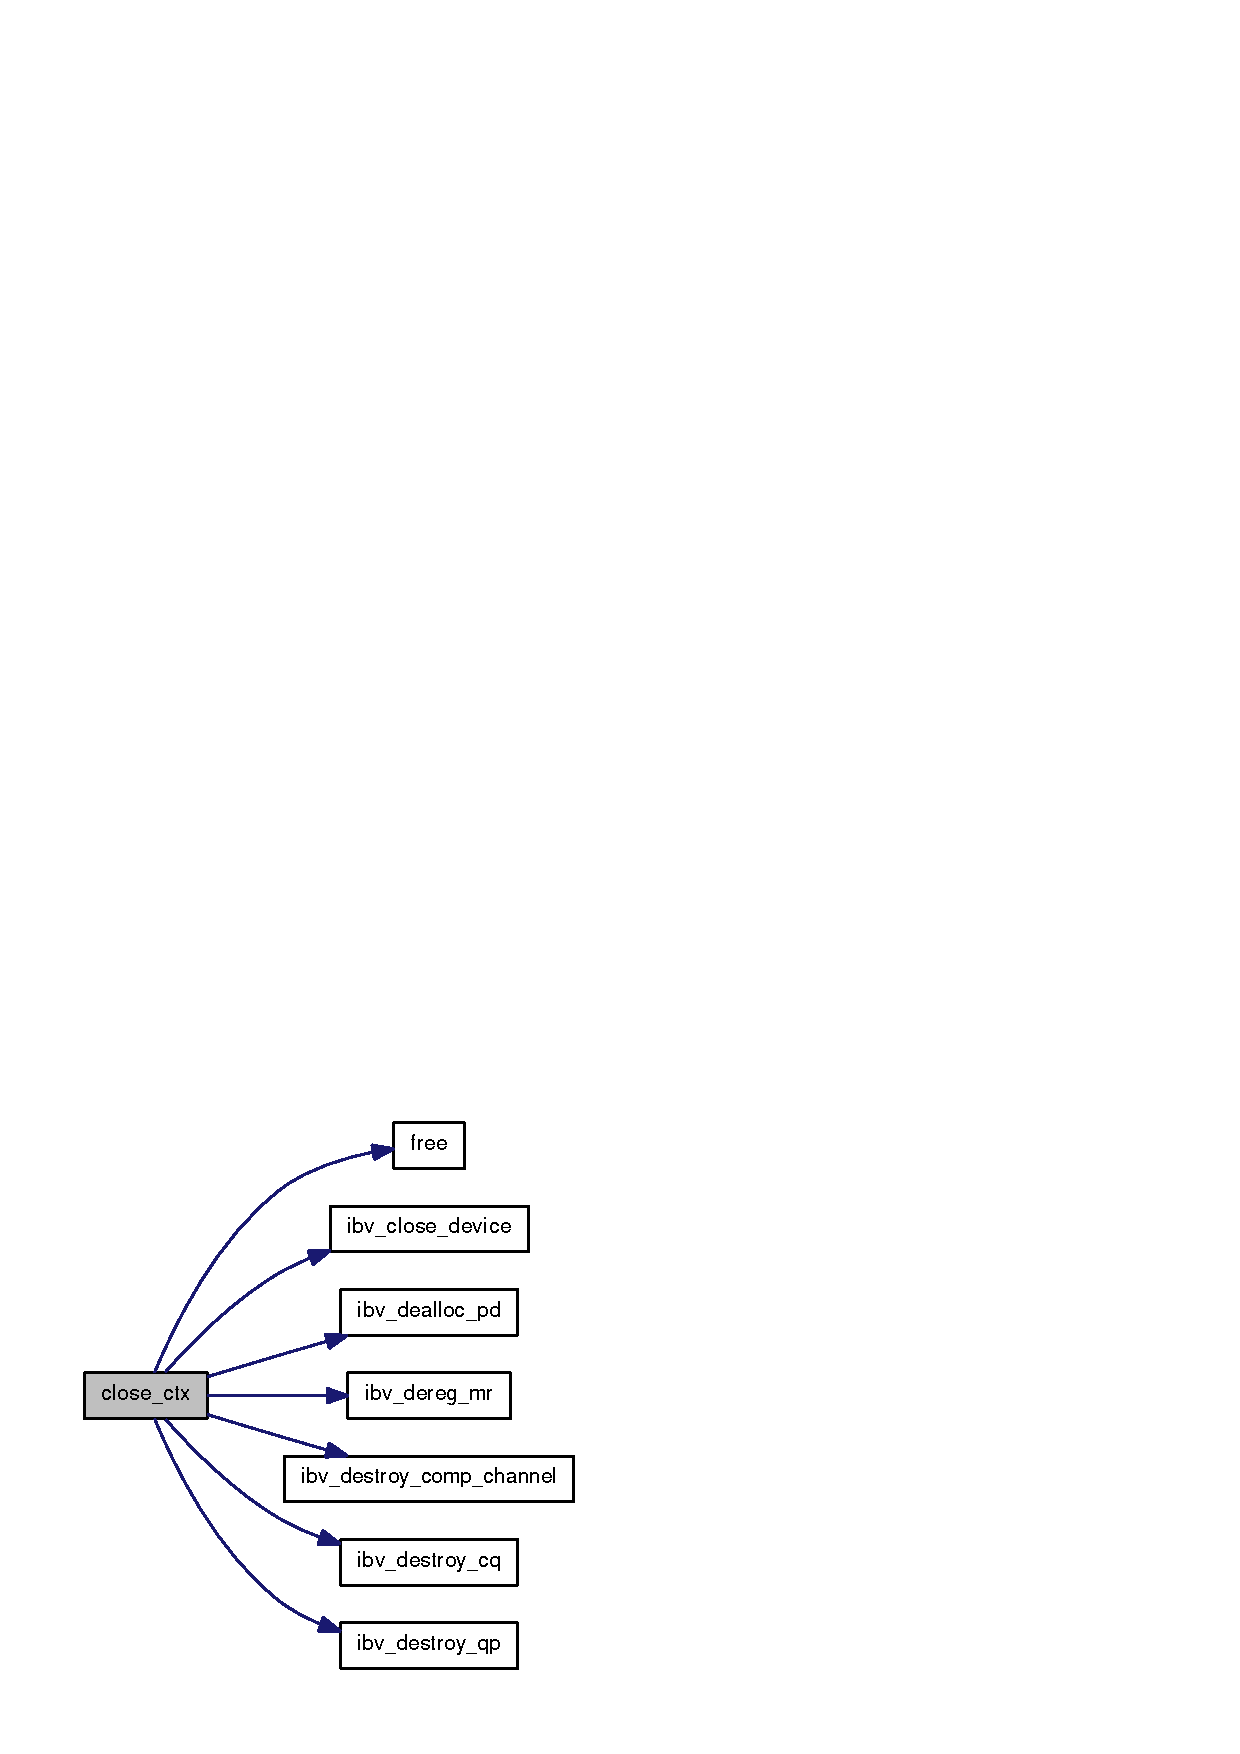
\includegraphics[width=140pt]{artem__rc__pingpong_8c_a7a76c3673a201262ddad0e6b4e7dab9c_cgraph}
\end{center}
\end{figure}


呼出しグラフ:\nopagebreak
\begin{figure}[H]
\begin{center}
\leavevmode
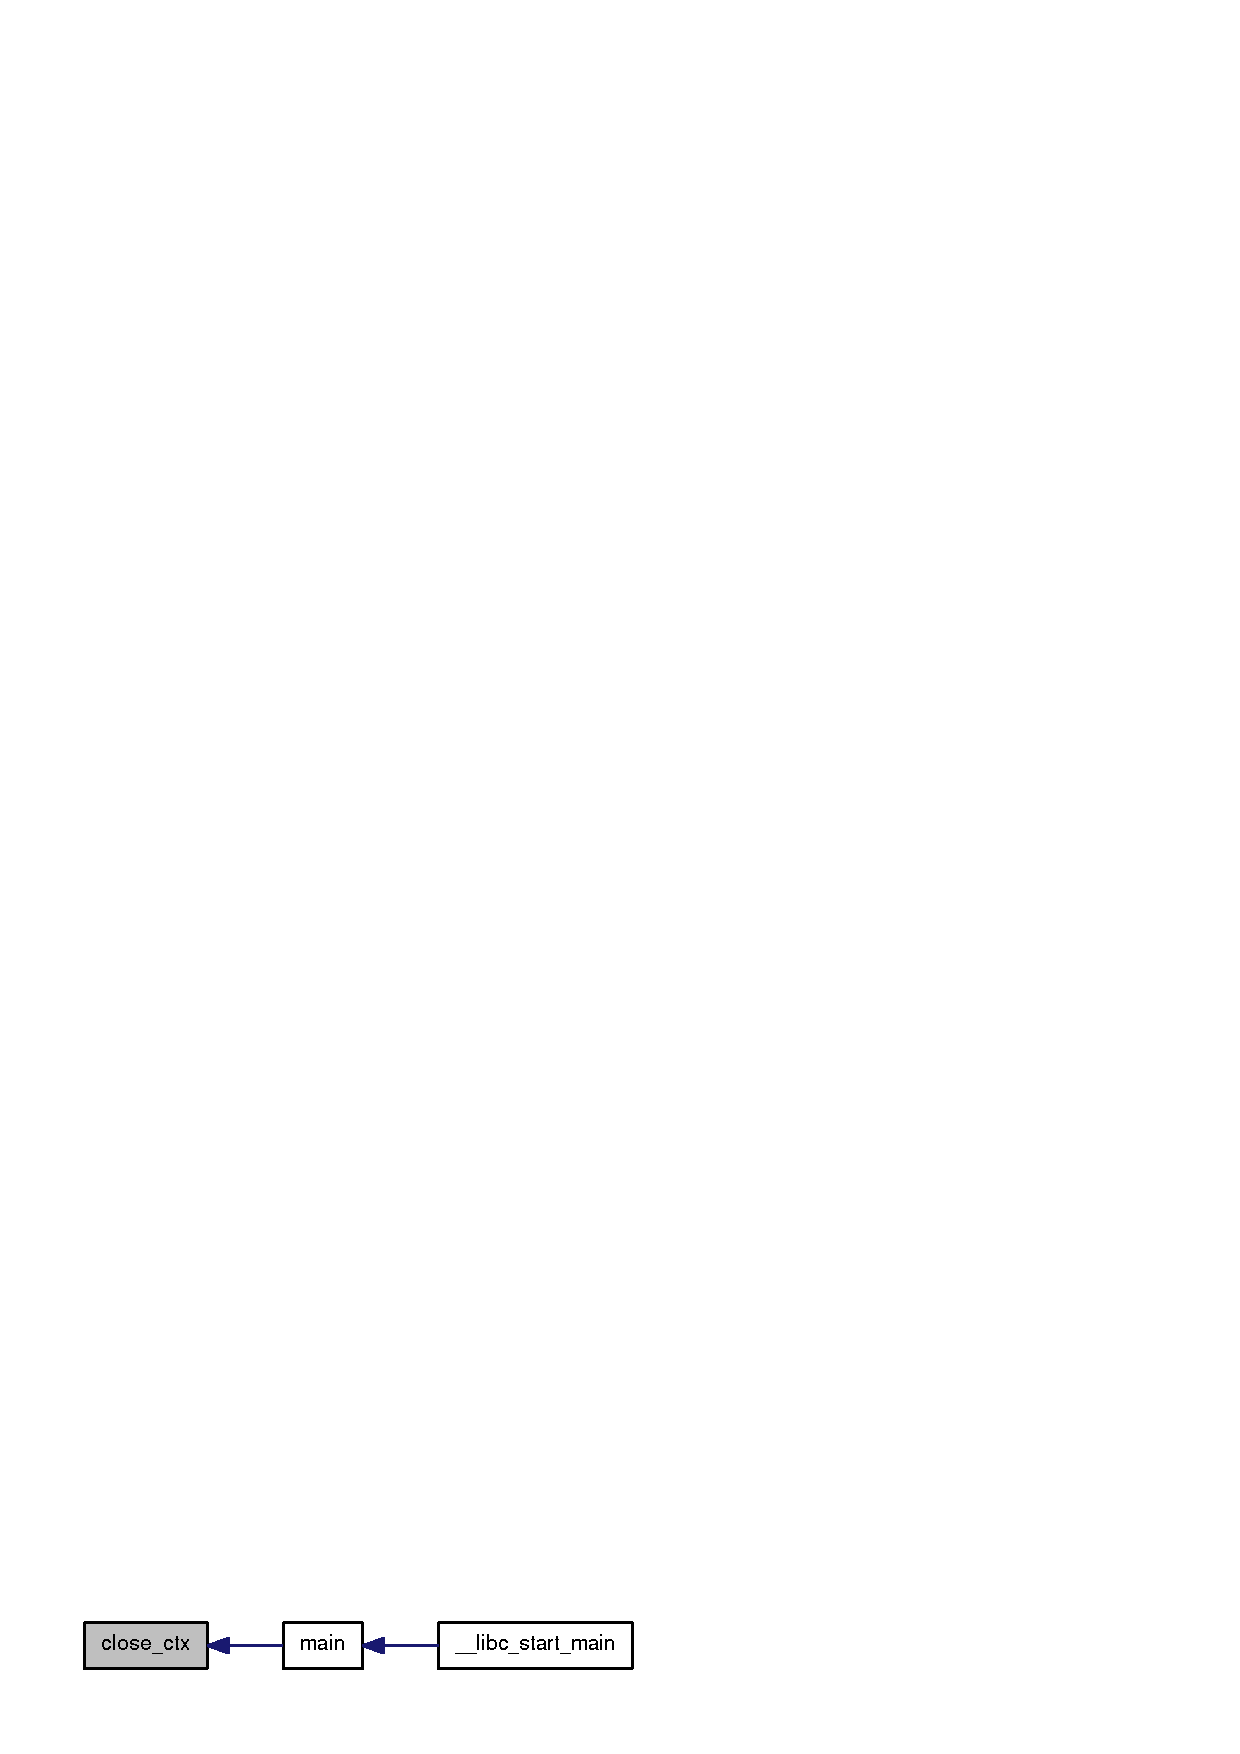
\includegraphics[width=154pt]{artem__rc__pingpong_8c_a7a76c3673a201262ddad0e6b4e7dab9c_icgraph}
\end{center}
\end{figure}
\hypertarget{artem__rc__pingpong_8c_a0ddf1224851353fc92bfbff6f499fa97}{
\index{artem\_\-rc\_\-pingpong.c@{artem\_\-rc\_\-pingpong.c}!main@{main}}
\index{main@{main}!artem_rc_pingpong.c@{artem\_\-rc\_\-pingpong.c}}
\subsubsection[{main}]{\setlength{\rightskip}{0pt plus 5cm}int main (int {\em argc}, \/  char $\ast$ {\em argv}\mbox{[}$\,$\mbox{]})}}
\label{artem__rc__pingpong_8c_a0ddf1224851353fc92bfbff6f499fa97}


関数の呼び出しグラフ:\nopagebreak
\begin{figure}[H]
\begin{center}
\leavevmode
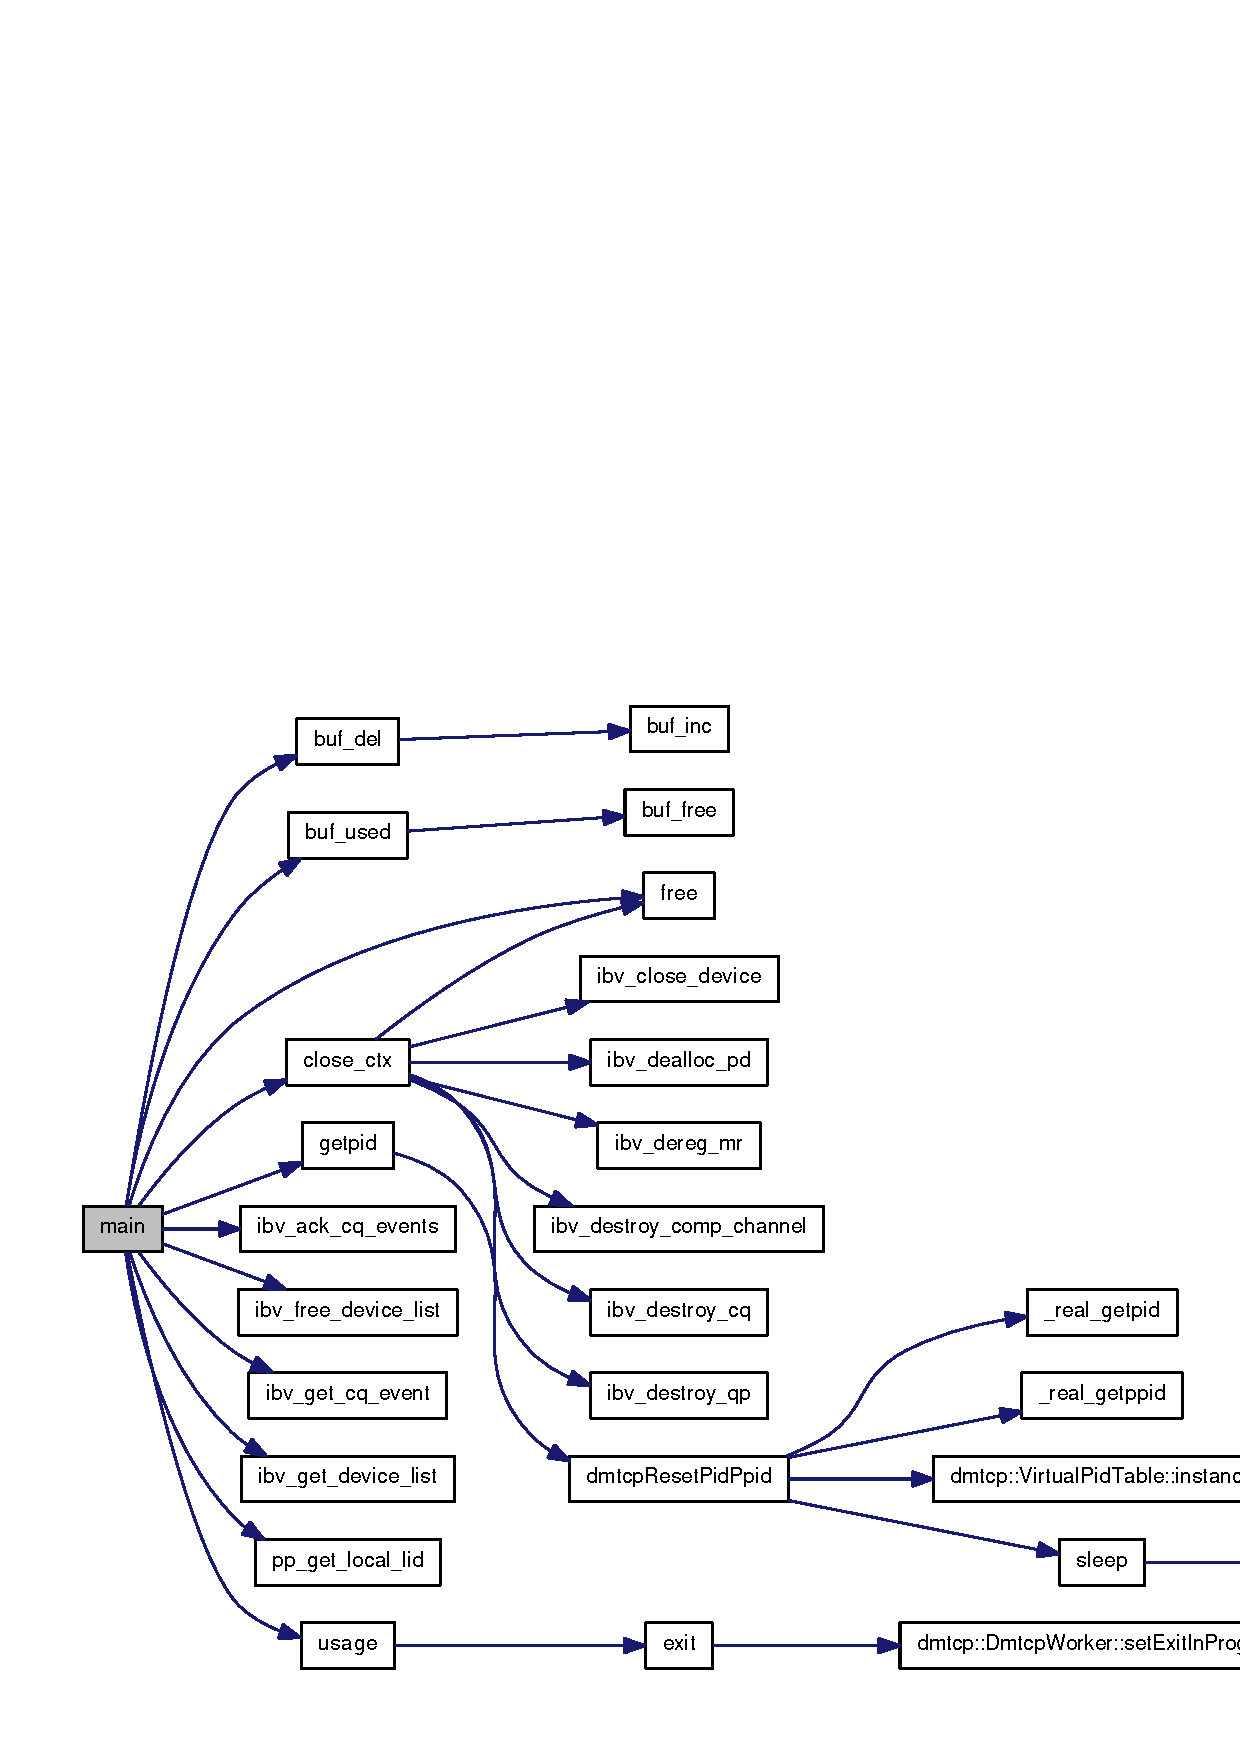
\includegraphics[width=420pt]{artem__rc__pingpong_8c_a0ddf1224851353fc92bfbff6f499fa97_cgraph}
\end{center}
\end{figure}


呼出しグラフ:\nopagebreak
\begin{figure}[H]
\begin{center}
\leavevmode
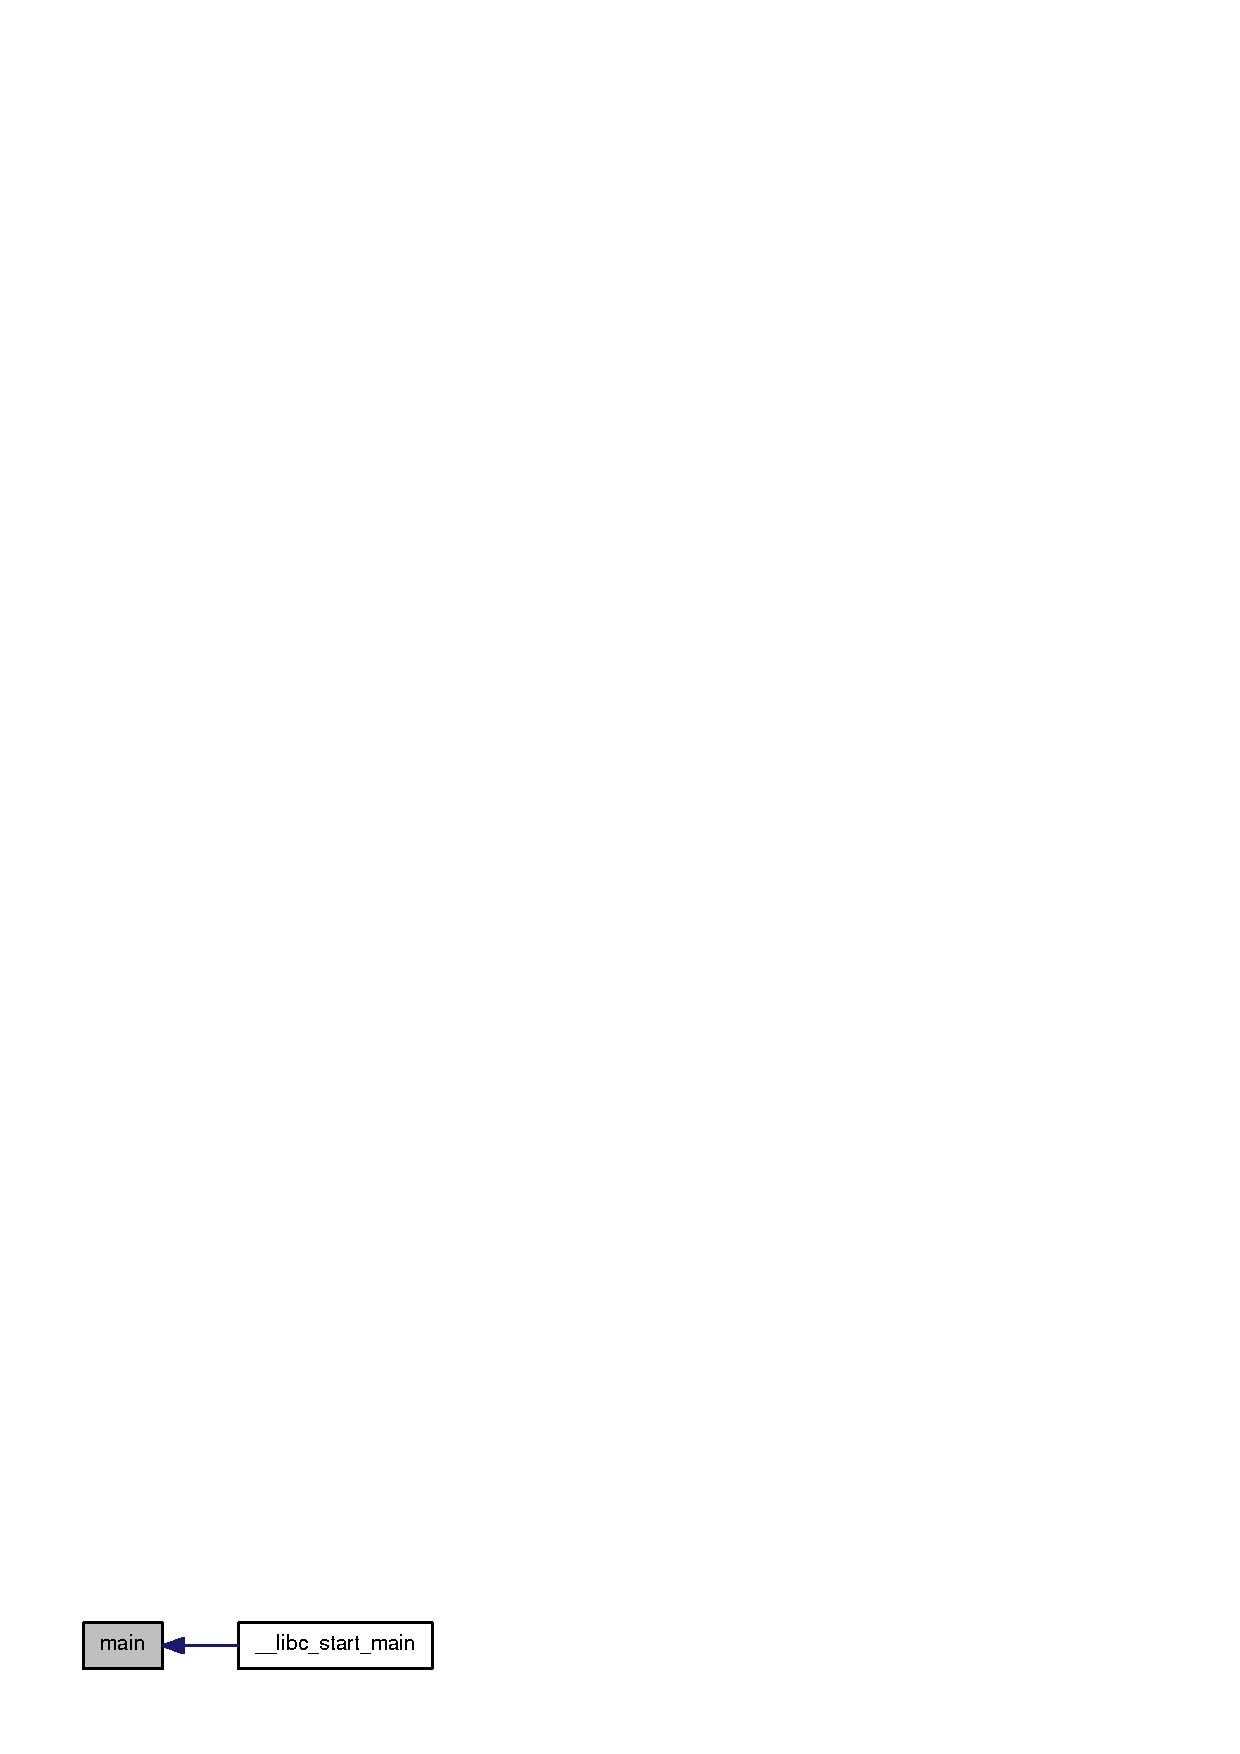
\includegraphics[width=106pt]{artem__rc__pingpong_8c_a0ddf1224851353fc92bfbff6f499fa97_icgraph}
\end{center}
\end{figure}


\subsection{変数}
\hypertarget{artem__rc__pingpong_8c_ac070153ead1986a5f0bed7b57ded8888}{
\index{artem\_\-rc\_\-pingpong.c@{artem\_\-rc\_\-pingpong.c}!local\_\-unack\_\-count@{local\_\-unack\_\-count}}
\index{local\_\-unack\_\-count@{local\_\-unack\_\-count}!artem_rc_pingpong.c@{artem\_\-rc\_\-pingpong.c}}
\subsubsection[{local\_\-unack\_\-count}]{\setlength{\rightskip}{0pt plus 5cm}{\bf uint} {\bf local\_\-unack\_\-count} = 0}}
\label{artem__rc__pingpong_8c_ac070153ead1986a5f0bed7b57ded8888}
\hypertarget{artem__rc__pingpong_8c_a7f508a72aa28dbdbfa0dc82d191c0983}{
\index{artem\_\-rc\_\-pingpong.c@{artem\_\-rc\_\-pingpong.c}!local\_\-unack\_\-tot@{local\_\-unack\_\-tot}}
\index{local\_\-unack\_\-tot@{local\_\-unack\_\-tot}!artem_rc_pingpong.c@{artem\_\-rc\_\-pingpong.c}}
\subsubsection[{local\_\-unack\_\-tot}]{\setlength{\rightskip}{0pt plus 5cm}{\bf uint} {\bf local\_\-unack\_\-tot} = 0}}
\label{artem__rc__pingpong_8c_a7f508a72aa28dbdbfa0dc82d191c0983}
\hypertarget{artem__rc__pingpong_8c_ad06efed141aae735dde3d59c3cf93890}{
\index{artem\_\-rc\_\-pingpong.c@{artem\_\-rc\_\-pingpong.c}!rem\_\-unack\_\-count@{rem\_\-unack\_\-count}}
\index{rem\_\-unack\_\-count@{rem\_\-unack\_\-count}!artem_rc_pingpong.c@{artem\_\-rc\_\-pingpong.c}}
\subsubsection[{rem\_\-unack\_\-count}]{\setlength{\rightskip}{0pt plus 5cm}{\bf uint} {\bf rem\_\-unack\_\-count} = 0}}
\label{artem__rc__pingpong_8c_ad06efed141aae735dde3d59c3cf93890}
\hypertarget{artem__rc__pingpong_8c_abab635a378d9ff76cbc0b91e997081e4}{
\index{artem\_\-rc\_\-pingpong.c@{artem\_\-rc\_\-pingpong.c}!rem\_\-unack\_\-tot@{rem\_\-unack\_\-tot}}
\index{rem\_\-unack\_\-tot@{rem\_\-unack\_\-tot}!artem_rc_pingpong.c@{artem\_\-rc\_\-pingpong.c}}
\subsubsection[{rem\_\-unack\_\-tot}]{\setlength{\rightskip}{0pt plus 5cm}{\bf uint} {\bf rem\_\-unack\_\-tot} = 0}}
\label{artem__rc__pingpong_8c_abab635a378d9ff76cbc0b91e997081e4}

\hypertarget{asyncwatch_8c}{
\section{contrib/infiniband/examples/asyncwatch.c}
\label{asyncwatch_8c}\index{contrib/infiniband/examples/asyncwatch.c@{contrib/infiniband/examples/asyncwatch.c}}
}
{\ttfamily \#include $<$stdio.h$>$}\par
{\ttfamily \#include $<$endian.h$>$}\par
{\ttfamily \#include $<$byteswap.h$>$}\par
{\ttfamily \#include $<$infiniband/verbs.h$>$}\par
asyncwatch.cのインクルード依存関係図\nopagebreak
\begin{figure}[H]
\begin{center}
\leavevmode
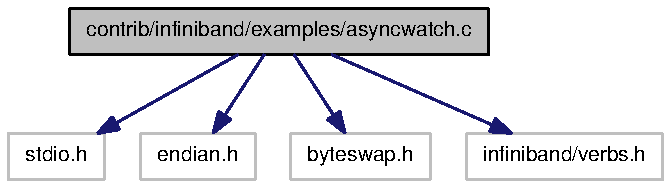
\includegraphics[width=179pt]{asyncwatch_8c__incl}
\end{center}
\end{figure}
\subsection*{関数}
\begin{DoxyCompactItemize}
\item 
int \hyperlink{asyncwatch_8c_a0ddf1224851353fc92bfbff6f499fa97}{main} (int argc, char $\ast$argv\mbox{[}$\,$\mbox{]})
\end{DoxyCompactItemize}


\subsection{関数}
\hypertarget{asyncwatch_8c_a0ddf1224851353fc92bfbff6f499fa97}{
\index{asyncwatch.c@{asyncwatch.c}!main@{main}}
\index{main@{main}!asyncwatch.c@{asyncwatch.c}}
\subsubsection[{main}]{\setlength{\rightskip}{0pt plus 5cm}int main (int {\em argc}, \/  char $\ast$ {\em argv}\mbox{[}$\,$\mbox{]})}}
\label{asyncwatch_8c_a0ddf1224851353fc92bfbff6f499fa97}


関数の呼び出しグラフ:\nopagebreak
\begin{figure}[H]
\begin{center}
\leavevmode
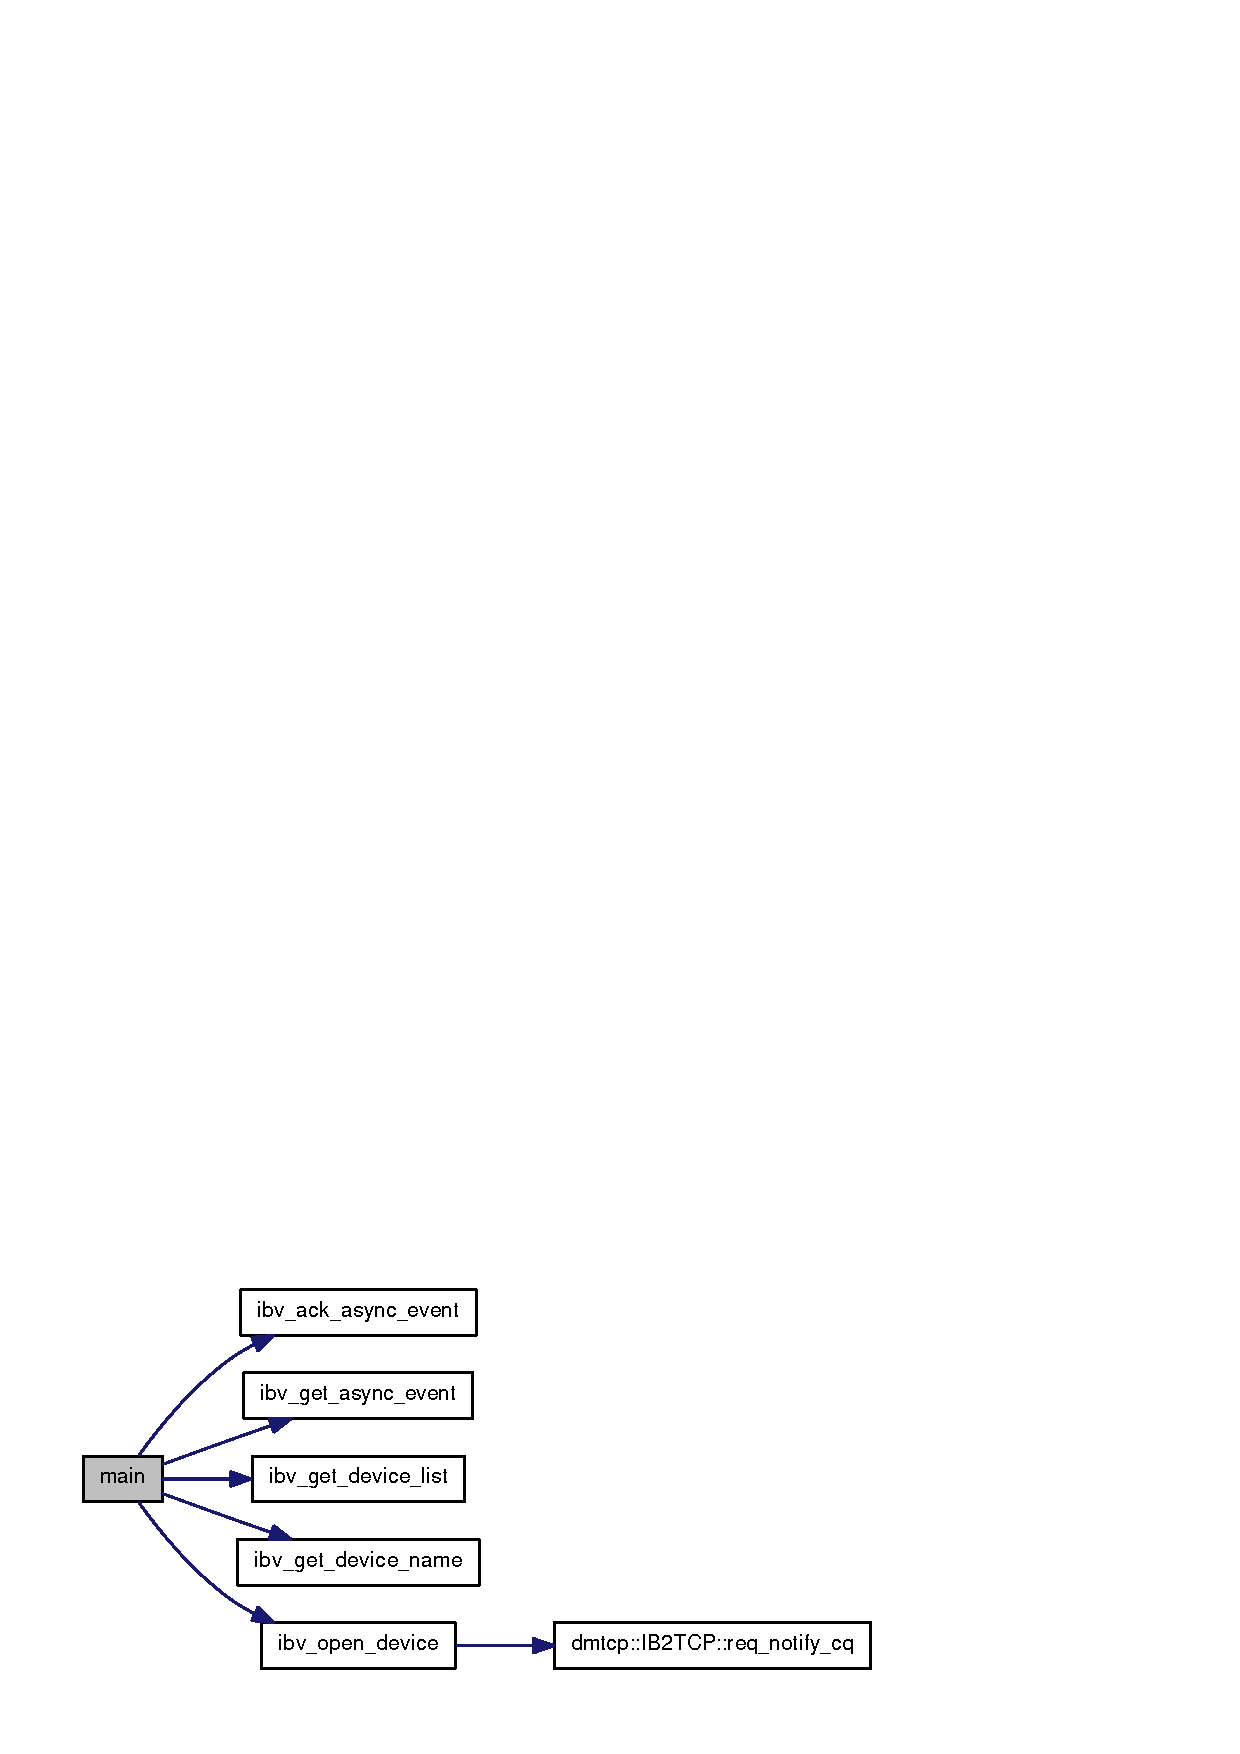
\includegraphics[width=211pt]{asyncwatch_8c_a0ddf1224851353fc92bfbff6f499fa97_cgraph}
\end{center}
\end{figure}

\hypertarget{device__list_8c}{
\section{contrib/infiniband/examples/device\_\-list.c}
\label{device__list_8c}\index{contrib/infiniband/examples/device\_\-list.c@{contrib/infiniband/examples/device\_\-list.c}}
}
{\ttfamily \#include $<$stdio.h$>$}\par
{\ttfamily \#include $<$endian.h$>$}\par
{\ttfamily \#include $<$byteswap.h$>$}\par
{\ttfamily \#include $<$infiniband/verbs.h$>$}\par
{\ttfamily \#include $<$infiniband/arch.h$>$}\par
device\_\-list.cのインクルード依存関係図\nopagebreak
\begin{figure}[H]
\begin{center}
\leavevmode
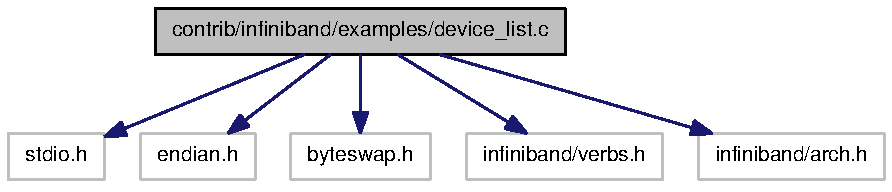
\includegraphics[width=232pt]{device__list_8c__incl}
\end{center}
\end{figure}
\subsection*{関数}
\begin{DoxyCompactItemize}
\item 
int \hyperlink{device__list_8c_a0ddf1224851353fc92bfbff6f499fa97}{main} (int argc, char $\ast$argv\mbox{[}$\,$\mbox{]})
\end{DoxyCompactItemize}


\subsection{関数}
\hypertarget{device__list_8c_a0ddf1224851353fc92bfbff6f499fa97}{
\index{device\_\-list.c@{device\_\-list.c}!main@{main}}
\index{main@{main}!device_list.c@{device\_\-list.c}}
\subsubsection[{main}]{\setlength{\rightskip}{0pt plus 5cm}int main (int {\em argc}, \/  char $\ast$ {\em argv}\mbox{[}$\,$\mbox{]})}}
\label{device__list_8c_a0ddf1224851353fc92bfbff6f499fa97}


関数の呼び出しグラフ:\nopagebreak
\begin{figure}[H]
\begin{center}
\leavevmode
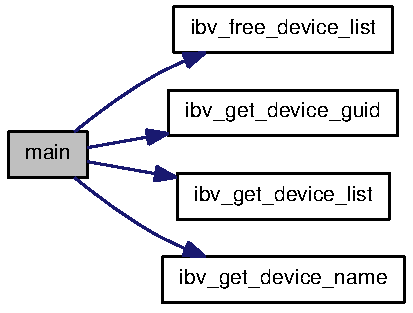
\includegraphics[width=117pt]{device__list_8c_a0ddf1224851353fc92bfbff6f499fa97_cgraph}
\end{center}
\end{figure}

\hypertarget{devinfo_8c}{
\section{contrib/infiniband/examples/devinfo.c}
\label{devinfo_8c}\index{contrib/infiniband/examples/devinfo.c@{contrib/infiniband/examples/devinfo.c}}
}
{\ttfamily \#include $<$stdio.h$>$}\par
{\ttfamily \#include $<$stdlib.h$>$}\par
{\ttfamily \#include $<$unistd.h$>$}\par
{\ttfamily \#include $<$string.h$>$}\par
{\ttfamily \#include $<$getopt.h$>$}\par
{\ttfamily \#include $<$netinet/in.h$>$}\par
{\ttfamily \#include $<$endian.h$>$}\par
{\ttfamily \#include $<$byteswap.h$>$}\par
{\ttfamily \#include $<$infiniband/verbs.h$>$}\par
{\ttfamily \#include $<$infiniband/driver.h$>$}\par
{\ttfamily \#include $<$infiniband/arch.h$>$}\par
devinfo.cのインクルード依存関係図\nopagebreak
\begin{figure}[H]
\begin{center}
\leavevmode
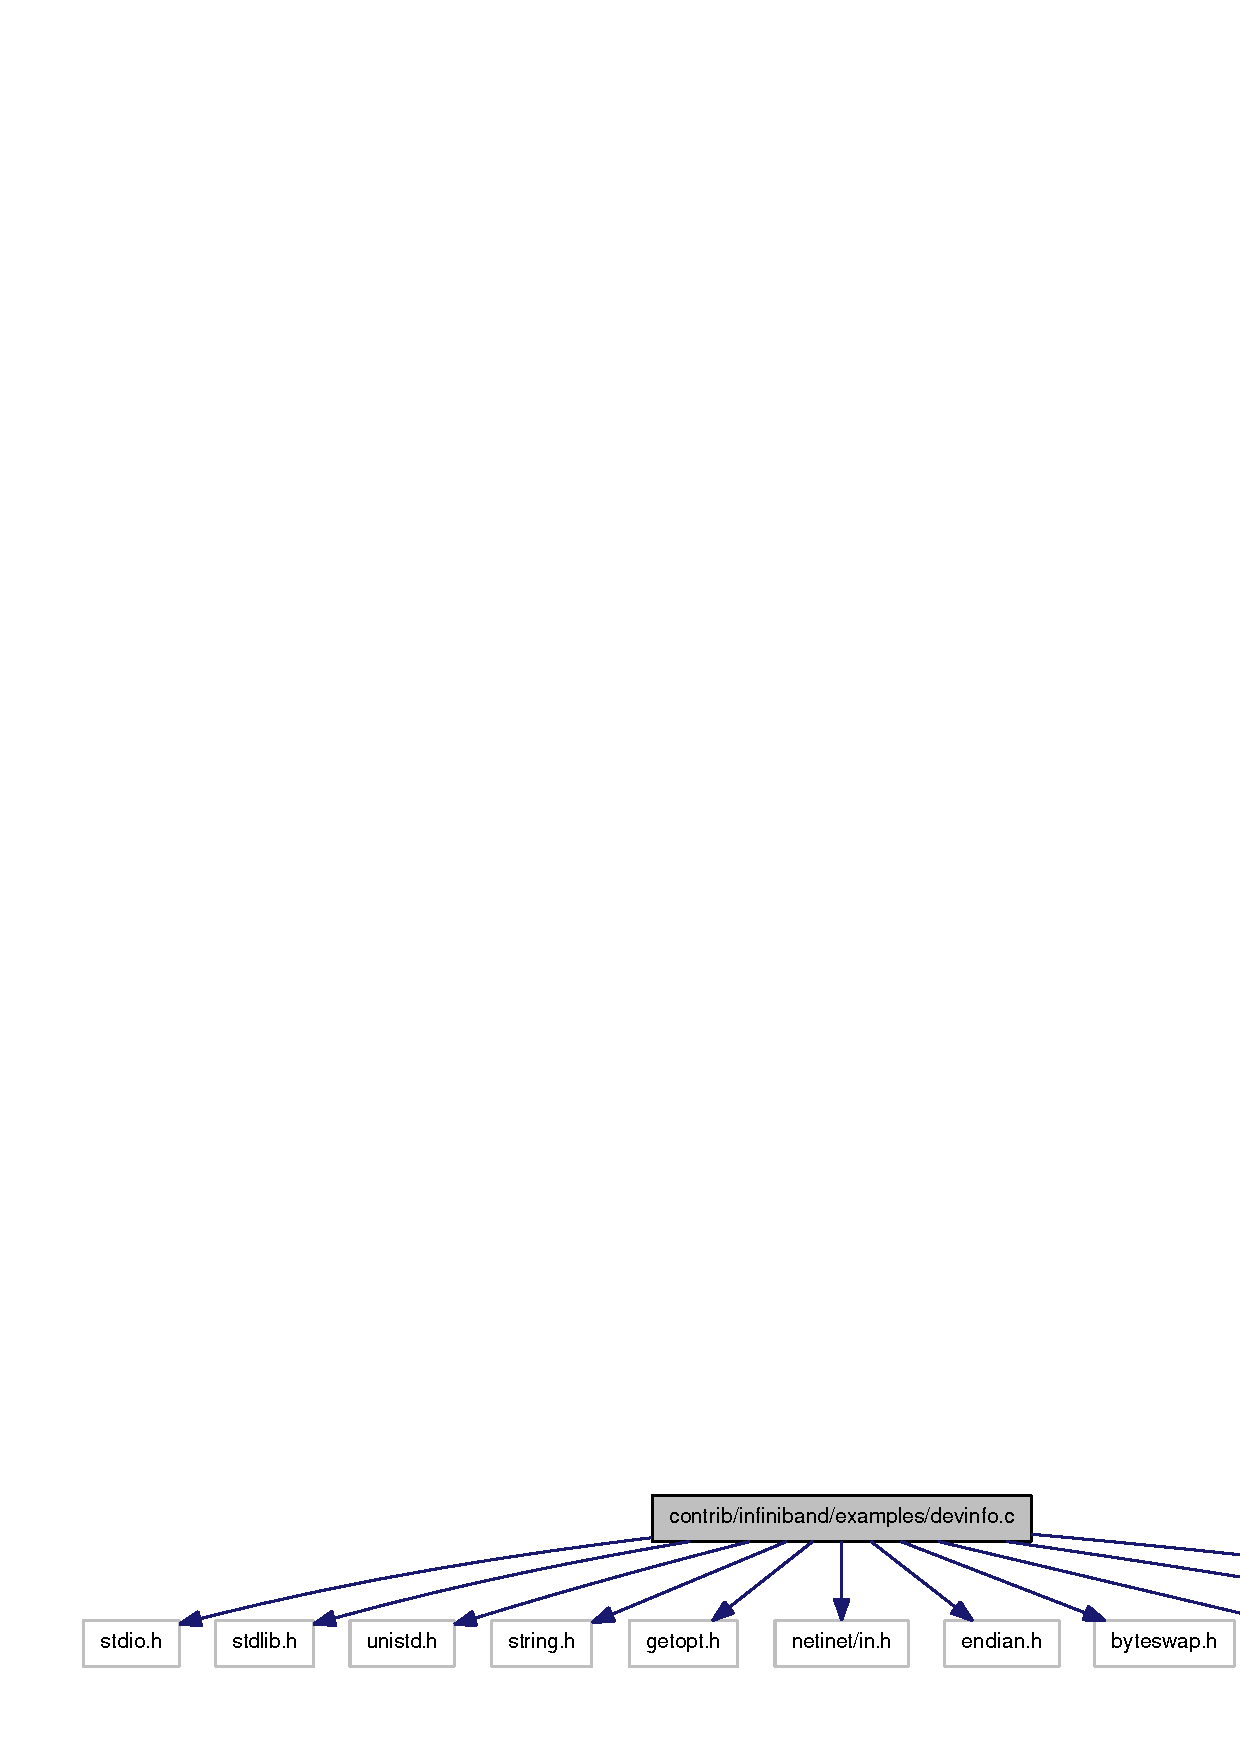
\includegraphics[width=420pt]{devinfo_8c__incl}
\end{center}
\end{figure}
\subsection*{関数}
\begin{DoxyCompactItemize}
\item 
int \hyperlink{devinfo_8c_a0ddf1224851353fc92bfbff6f499fa97}{main} (int argc, char $\ast$argv\mbox{[}$\,$\mbox{]})
\end{DoxyCompactItemize}


\subsection{関数}
\hypertarget{devinfo_8c_a0ddf1224851353fc92bfbff6f499fa97}{
\index{devinfo.c@{devinfo.c}!main@{main}}
\index{main@{main}!devinfo.c@{devinfo.c}}
\subsubsection[{main}]{\setlength{\rightskip}{0pt plus 5cm}int main (int {\em argc}, \/  char $\ast$ {\em argv}\mbox{[}$\,$\mbox{]})}}
\label{devinfo_8c_a0ddf1224851353fc92bfbff6f499fa97}


関数の呼び出しグラフ:\nopagebreak
\begin{figure}[H]
\begin{center}
\leavevmode
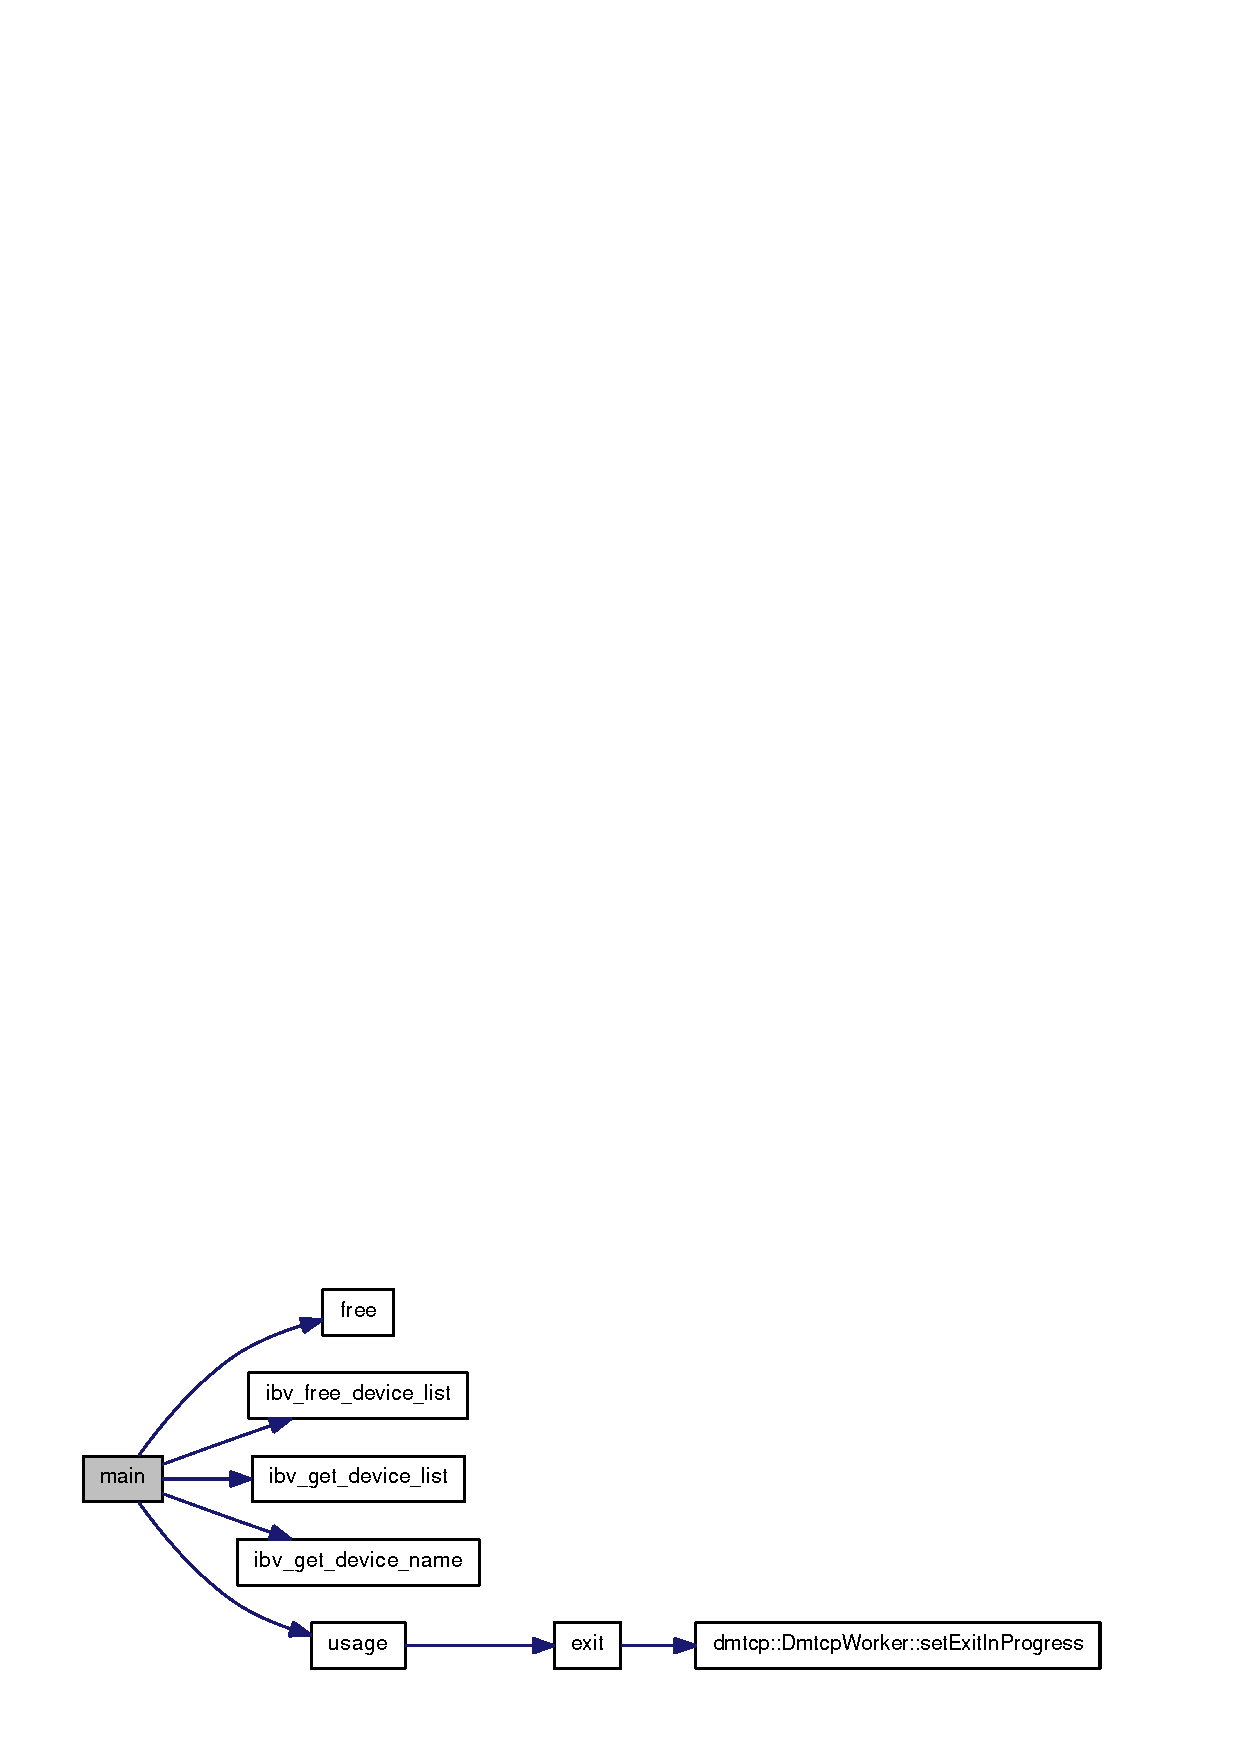
\includegraphics[width=266pt]{devinfo_8c_a0ddf1224851353fc92bfbff6f499fa97_cgraph}
\end{center}
\end{figure}

\hypertarget{pingpong_8c}{
\section{contrib/infiniband/examples/pingpong.c}
\label{pingpong_8c}\index{contrib/infiniband/examples/pingpong.c@{contrib/infiniband/examples/pingpong.c}}
}
{\ttfamily \#include \char`\"{}pingpong.h\char`\"{}}\par
{\ttfamily \#include $<$arpa/inet.h$>$}\par
{\ttfamily \#include $<$stdlib.h$>$}\par
{\ttfamily \#include $<$stdio.h$>$}\par
{\ttfamily \#include $<$string.h$>$}\par
pingpong.cのインクルード依存関係図\nopagebreak
\begin{figure}[H]
\begin{center}
\leavevmode
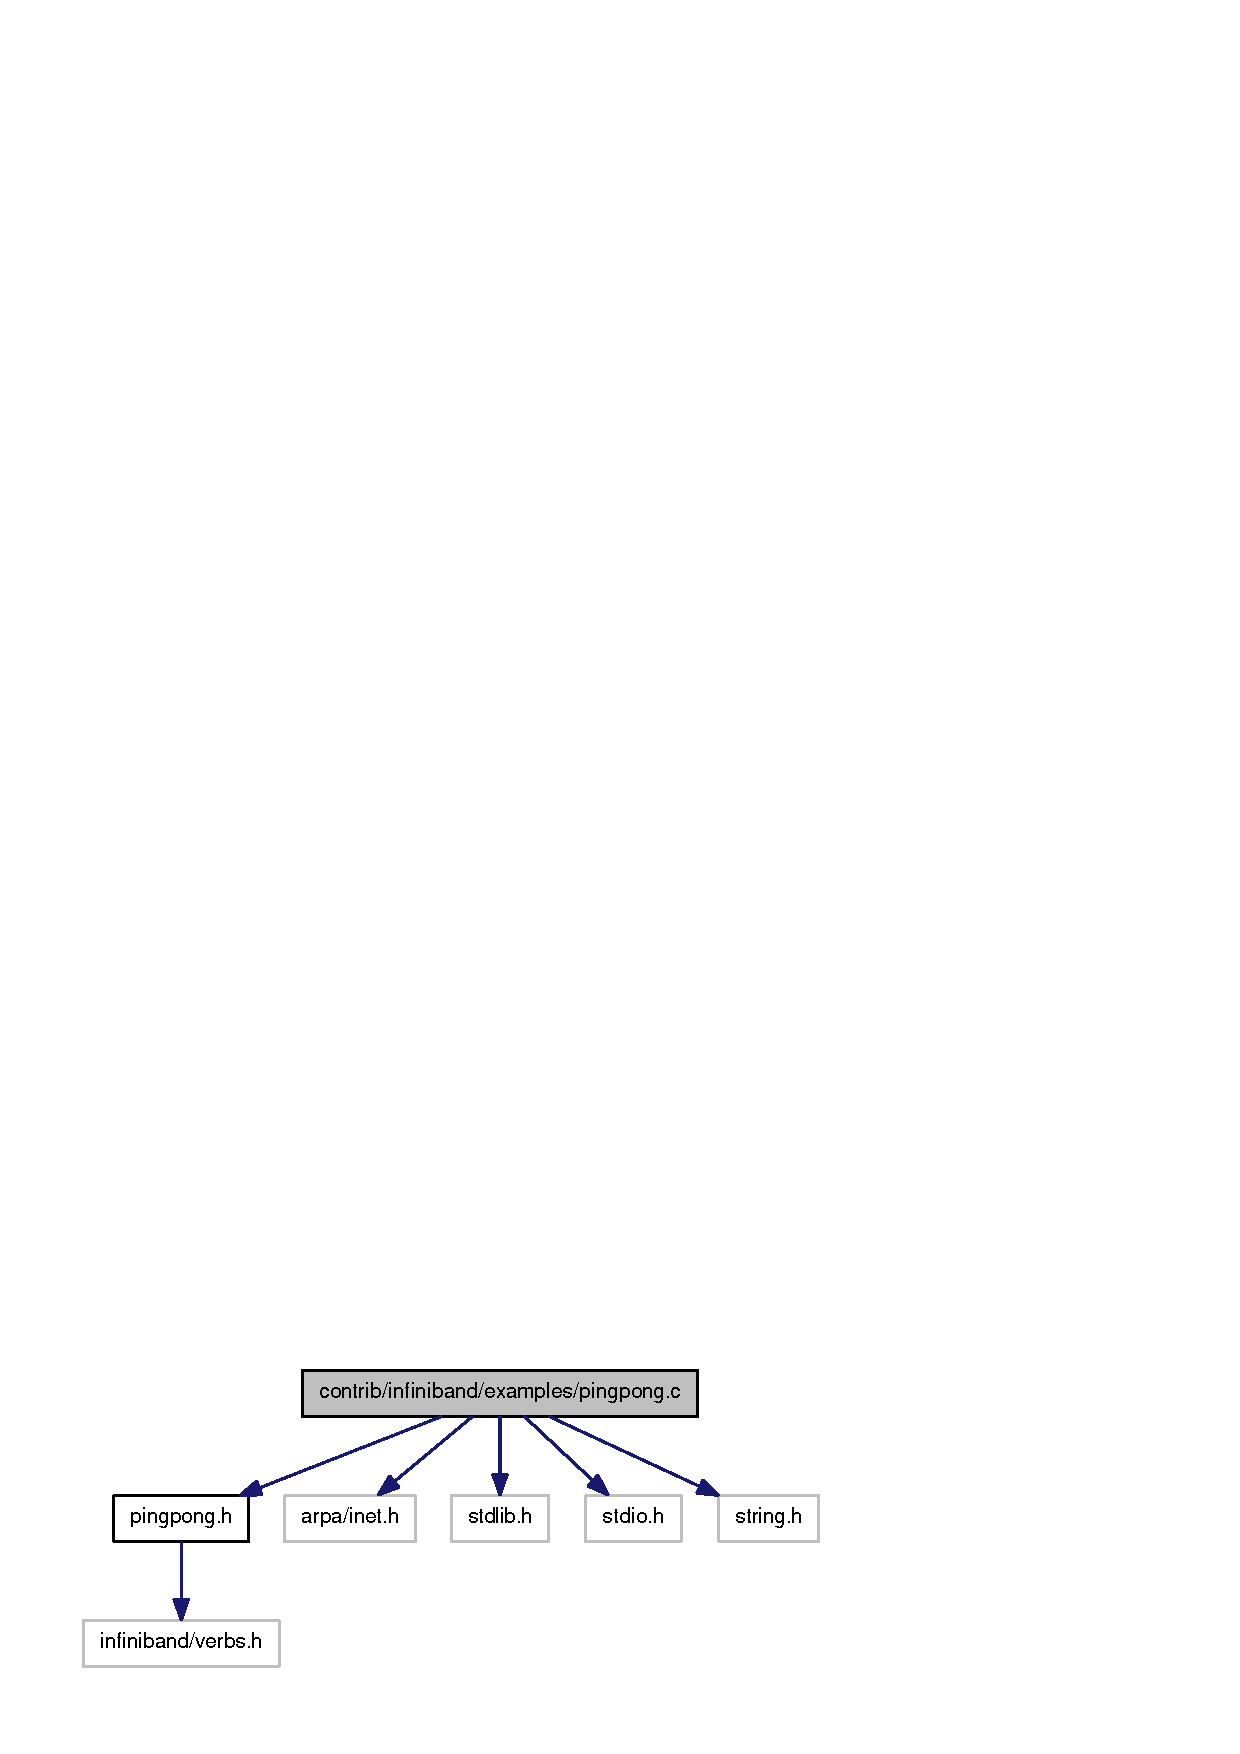
\includegraphics[width=198pt]{pingpong_8c__incl}
\end{center}
\end{figure}
\subsection*{関数}
\begin{DoxyCompactItemize}
\item 
enum ibv\_\-mtu \hyperlink{pingpong_8c_a33e1c8a476557b41756d0e417b1056b4}{pp\_\-mtu\_\-to\_\-enum} (int mtu)
\item 
uint16\_\-t \hyperlink{pingpong_8c_a0e318c8b87253380ec891a6372515a28}{pp\_\-get\_\-local\_\-lid} (struct ibv\_\-context $\ast$\hyperlink{structcontext}{context}, int port)
\item 
int \hyperlink{pingpong_8c_ab1ab3764c449c63a0d98caeb8ec5458e}{pp\_\-get\_\-port\_\-info} (struct ibv\_\-context $\ast$\hyperlink{structcontext}{context}, int port, struct ibv\_\-port\_\-attr $\ast$attr)
\item 
void \hyperlink{pingpong_8c_aab36fd488327288bd176f34544648b70}{wire\_\-gid\_\-to\_\-gid} (const char $\ast$wgid, union ibv\_\-gid $\ast$gid)
\item 
void \hyperlink{pingpong_8c_a2b4e53497de0ba125ad41bc77d25c1ef}{gid\_\-to\_\-wire\_\-gid} (const union ibv\_\-gid $\ast$gid, char wgid\mbox{[}$\,$\mbox{]})
\end{DoxyCompactItemize}


\subsection{関数}
\hypertarget{pingpong_8c_a2b4e53497de0ba125ad41bc77d25c1ef}{
\index{pingpong.c@{pingpong.c}!gid\_\-to\_\-wire\_\-gid@{gid\_\-to\_\-wire\_\-gid}}
\index{gid\_\-to\_\-wire\_\-gid@{gid\_\-to\_\-wire\_\-gid}!pingpong.c@{pingpong.c}}
\subsubsection[{gid\_\-to\_\-wire\_\-gid}]{\setlength{\rightskip}{0pt plus 5cm}void gid\_\-to\_\-wire\_\-gid (const union ibv\_\-gid $\ast$ {\em gid}, \/  char {\em wgid}\mbox{[}$\,$\mbox{]})}}
\label{pingpong_8c_a2b4e53497de0ba125ad41bc77d25c1ef}
\hypertarget{pingpong_8c_a0e318c8b87253380ec891a6372515a28}{
\index{pingpong.c@{pingpong.c}!pp\_\-get\_\-local\_\-lid@{pp\_\-get\_\-local\_\-lid}}
\index{pp\_\-get\_\-local\_\-lid@{pp\_\-get\_\-local\_\-lid}!pingpong.c@{pingpong.c}}
\subsubsection[{pp\_\-get\_\-local\_\-lid}]{\setlength{\rightskip}{0pt plus 5cm}uint16\_\-t pp\_\-get\_\-local\_\-lid (struct ibv\_\-context $\ast$ {\em context}, \/  int {\em port})}}
\label{pingpong_8c_a0e318c8b87253380ec891a6372515a28}


呼出しグラフ:\nopagebreak
\begin{figure}[H]
\begin{center}
\leavevmode
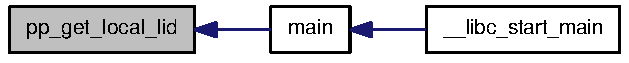
\includegraphics[width=169pt]{pingpong_8c_a0e318c8b87253380ec891a6372515a28_icgraph}
\end{center}
\end{figure}
\hypertarget{pingpong_8c_ab1ab3764c449c63a0d98caeb8ec5458e}{
\index{pingpong.c@{pingpong.c}!pp\_\-get\_\-port\_\-info@{pp\_\-get\_\-port\_\-info}}
\index{pp\_\-get\_\-port\_\-info@{pp\_\-get\_\-port\_\-info}!pingpong.c@{pingpong.c}}
\subsubsection[{pp\_\-get\_\-port\_\-info}]{\setlength{\rightskip}{0pt plus 5cm}int pp\_\-get\_\-port\_\-info (struct ibv\_\-context $\ast$ {\em context}, \/  int {\em port}, \/  struct ibv\_\-port\_\-attr $\ast$ {\em attr})}}
\label{pingpong_8c_ab1ab3764c449c63a0d98caeb8ec5458e}


呼出しグラフ:\nopagebreak
\begin{figure}[H]
\begin{center}
\leavevmode
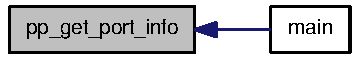
\includegraphics[width=104pt]{pingpong_8c_ab1ab3764c449c63a0d98caeb8ec5458e_icgraph}
\end{center}
\end{figure}
\hypertarget{pingpong_8c_a33e1c8a476557b41756d0e417b1056b4}{
\index{pingpong.c@{pingpong.c}!pp\_\-mtu\_\-to\_\-enum@{pp\_\-mtu\_\-to\_\-enum}}
\index{pp\_\-mtu\_\-to\_\-enum@{pp\_\-mtu\_\-to\_\-enum}!pingpong.c@{pingpong.c}}
\subsubsection[{pp\_\-mtu\_\-to\_\-enum}]{\setlength{\rightskip}{0pt plus 5cm}enum ibv\_\-mtu pp\_\-mtu\_\-to\_\-enum (int {\em mtu})}}
\label{pingpong_8c_a33e1c8a476557b41756d0e417b1056b4}


呼出しグラフ:\nopagebreak
\begin{figure}[H]
\begin{center}
\leavevmode
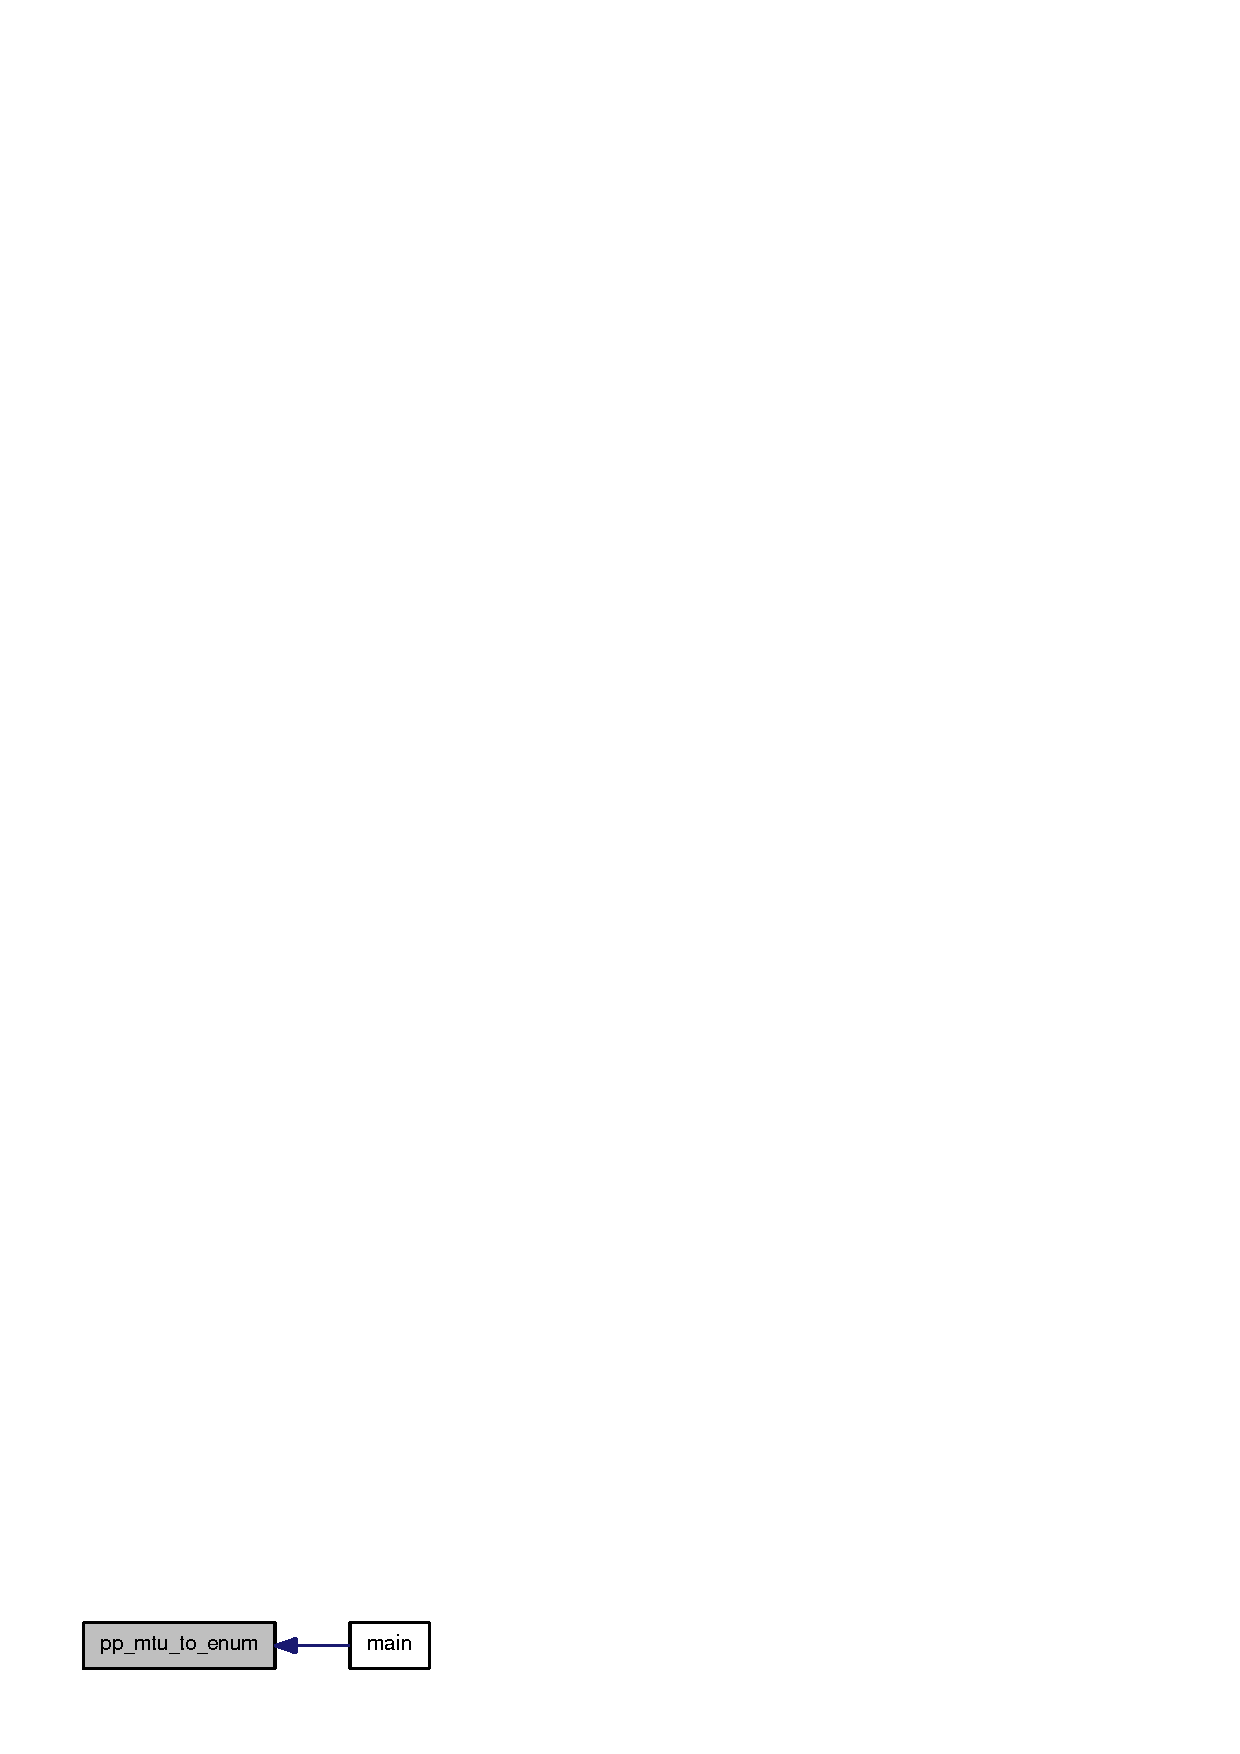
\includegraphics[width=105pt]{pingpong_8c_a33e1c8a476557b41756d0e417b1056b4_icgraph}
\end{center}
\end{figure}
\hypertarget{pingpong_8c_aab36fd488327288bd176f34544648b70}{
\index{pingpong.c@{pingpong.c}!wire\_\-gid\_\-to\_\-gid@{wire\_\-gid\_\-to\_\-gid}}
\index{wire\_\-gid\_\-to\_\-gid@{wire\_\-gid\_\-to\_\-gid}!pingpong.c@{pingpong.c}}
\subsubsection[{wire\_\-gid\_\-to\_\-gid}]{\setlength{\rightskip}{0pt plus 5cm}void wire\_\-gid\_\-to\_\-gid (const char $\ast$ {\em wgid}, \/  union ibv\_\-gid $\ast$ {\em gid})}}
\label{pingpong_8c_aab36fd488327288bd176f34544648b70}


関数の呼び出しグラフ:\nopagebreak
\begin{figure}[H]
\begin{center}
\leavevmode
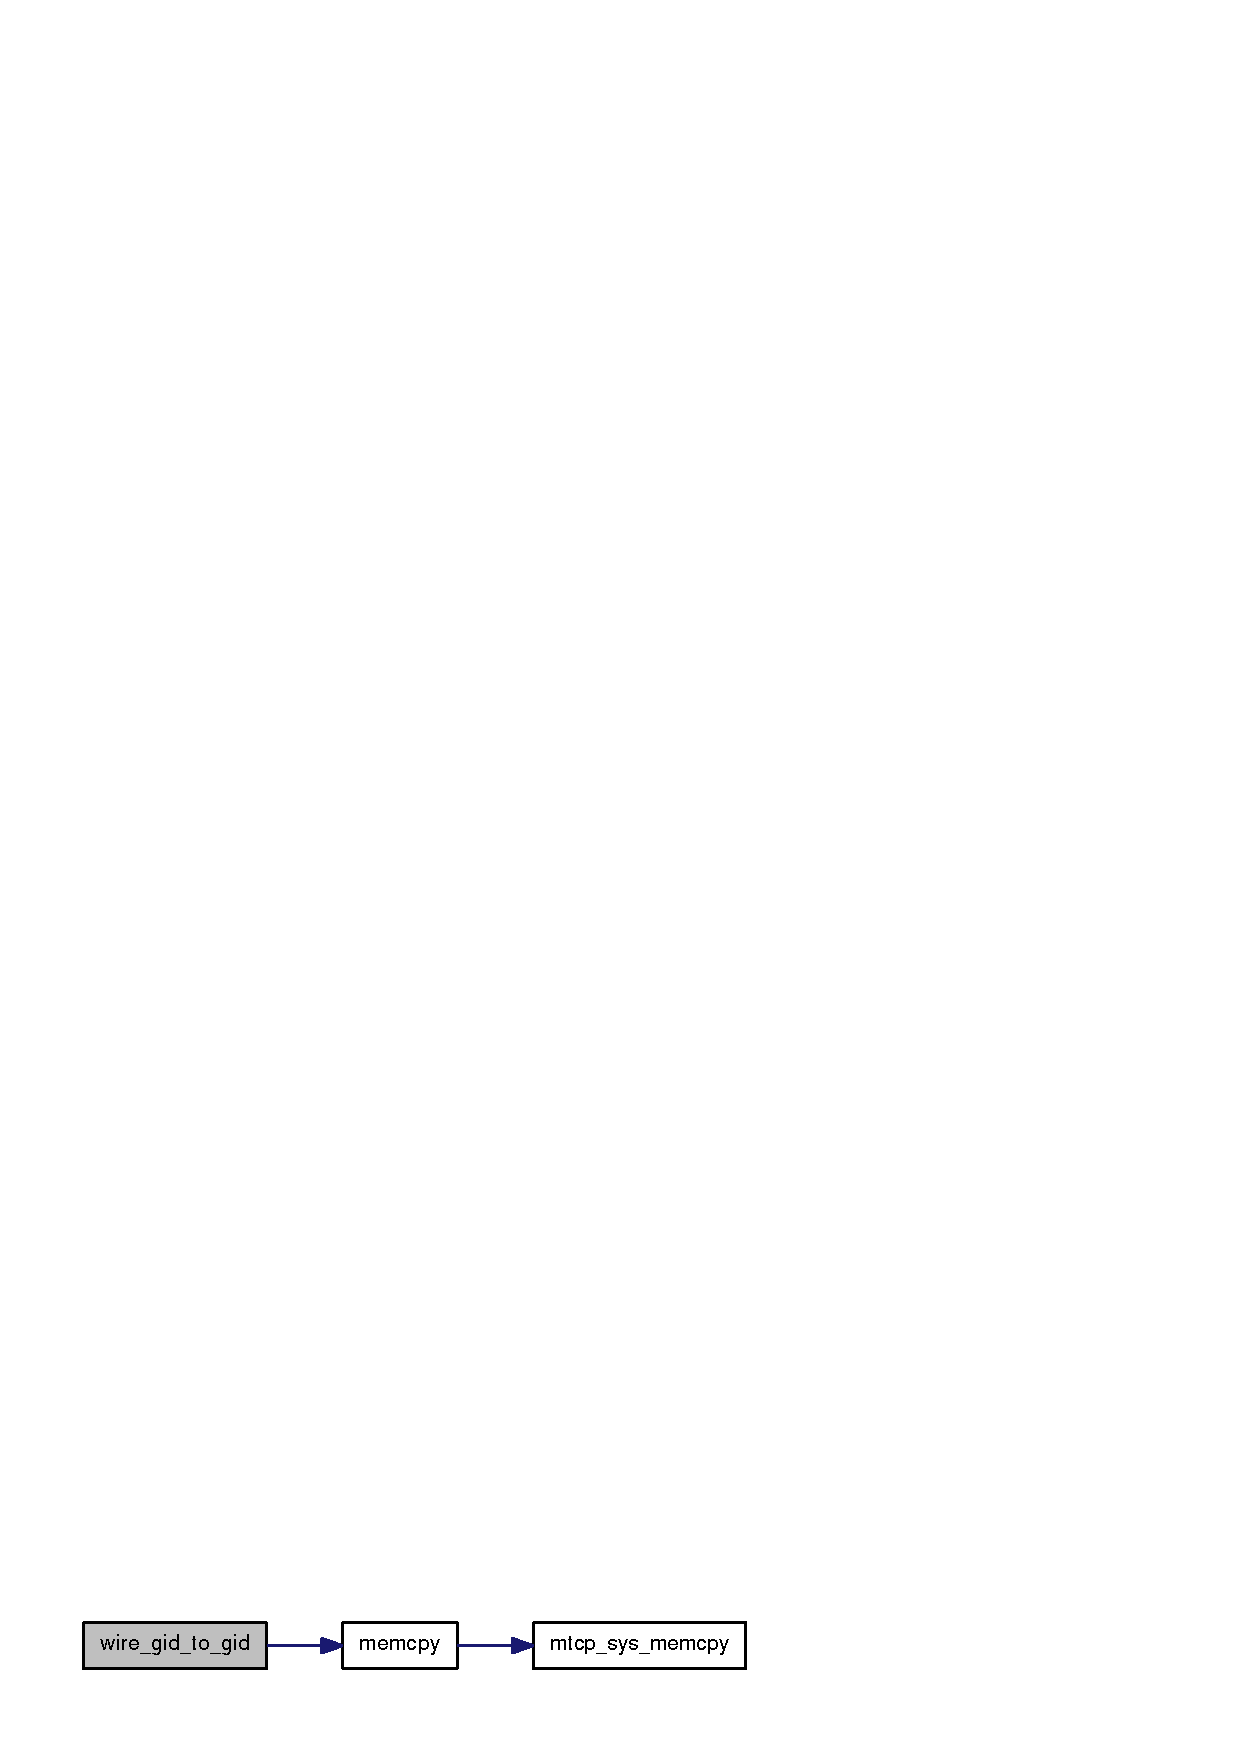
\includegraphics[width=181pt]{pingpong_8c_aab36fd488327288bd176f34544648b70_cgraph}
\end{center}
\end{figure}

\hypertarget{pingpong_8h}{
\section{contrib/infiniband/examples/pingpong.h}
\label{pingpong_8h}\index{contrib/infiniband/examples/pingpong.h@{contrib/infiniband/examples/pingpong.h}}
}
{\ttfamily \#include $<$infiniband/verbs.h$>$}\par
pingpong.hのインクルード依存関係図\nopagebreak
\begin{figure}[H]
\begin{center}
\leavevmode
\includegraphics[width=117pt]{pingpong_8h__incl}
\end{center}
\end{figure}
このグラフは、どのファイルから直接、間接的にインクルードされているかを示しています。\nopagebreak
\begin{figure}[H]
\begin{center}
\leavevmode
\includegraphics[width=420pt]{pingpong_8h__dep__incl}
\end{center}
\end{figure}
\subsection*{関数}
\begin{DoxyCompactItemize}
\item 
enum ibv\_\-mtu \hyperlink{pingpong_8h_a33e1c8a476557b41756d0e417b1056b4}{pp\_\-mtu\_\-to\_\-enum} (int mtu)
\item 
uint16\_\-t \hyperlink{pingpong_8h_a0e318c8b87253380ec891a6372515a28}{pp\_\-get\_\-local\_\-lid} (struct ibv\_\-context $\ast$\hyperlink{structcontext}{context}, int port)
\item 
int \hyperlink{pingpong_8h_ab1ab3764c449c63a0d98caeb8ec5458e}{pp\_\-get\_\-port\_\-info} (struct ibv\_\-context $\ast$\hyperlink{structcontext}{context}, int port, struct ibv\_\-port\_\-attr $\ast$attr)
\item 
void \hyperlink{pingpong_8h_aab36fd488327288bd176f34544648b70}{wire\_\-gid\_\-to\_\-gid} (const char $\ast$wgid, union ibv\_\-gid $\ast$gid)
\item 
void \hyperlink{pingpong_8h_a2b4e53497de0ba125ad41bc77d25c1ef}{gid\_\-to\_\-wire\_\-gid} (const union ibv\_\-gid $\ast$gid, char wgid\mbox{[}$\,$\mbox{]})
\end{DoxyCompactItemize}


\subsection{関数}
\hypertarget{pingpong_8h_a2b4e53497de0ba125ad41bc77d25c1ef}{
\index{pingpong.h@{pingpong.h}!gid\_\-to\_\-wire\_\-gid@{gid\_\-to\_\-wire\_\-gid}}
\index{gid\_\-to\_\-wire\_\-gid@{gid\_\-to\_\-wire\_\-gid}!pingpong.h@{pingpong.h}}
\subsubsection[{gid\_\-to\_\-wire\_\-gid}]{\setlength{\rightskip}{0pt plus 5cm}void gid\_\-to\_\-wire\_\-gid (const union ibv\_\-gid $\ast$ {\em gid}, \/  char {\em wgid}\mbox{[}$\,$\mbox{]})}}
\label{pingpong_8h_a2b4e53497de0ba125ad41bc77d25c1ef}
\hypertarget{pingpong_8h_a0e318c8b87253380ec891a6372515a28}{
\index{pingpong.h@{pingpong.h}!pp\_\-get\_\-local\_\-lid@{pp\_\-get\_\-local\_\-lid}}
\index{pp\_\-get\_\-local\_\-lid@{pp\_\-get\_\-local\_\-lid}!pingpong.h@{pingpong.h}}
\subsubsection[{pp\_\-get\_\-local\_\-lid}]{\setlength{\rightskip}{0pt plus 5cm}uint16\_\-t pp\_\-get\_\-local\_\-lid (struct ibv\_\-context $\ast$ {\em context}, \/  int {\em port})}}
\label{pingpong_8h_a0e318c8b87253380ec891a6372515a28}


呼出しグラフ:\nopagebreak
\begin{figure}[H]
\begin{center}
\leavevmode
\includegraphics[width=169pt]{pingpong_8h_a0e318c8b87253380ec891a6372515a28_icgraph}
\end{center}
\end{figure}
\hypertarget{pingpong_8h_ab1ab3764c449c63a0d98caeb8ec5458e}{
\index{pingpong.h@{pingpong.h}!pp\_\-get\_\-port\_\-info@{pp\_\-get\_\-port\_\-info}}
\index{pp\_\-get\_\-port\_\-info@{pp\_\-get\_\-port\_\-info}!pingpong.h@{pingpong.h}}
\subsubsection[{pp\_\-get\_\-port\_\-info}]{\setlength{\rightskip}{0pt plus 5cm}int pp\_\-get\_\-port\_\-info (struct ibv\_\-context $\ast$ {\em context}, \/  int {\em port}, \/  struct ibv\_\-port\_\-attr $\ast$ {\em attr})}}
\label{pingpong_8h_ab1ab3764c449c63a0d98caeb8ec5458e}


呼出しグラフ:\nopagebreak
\begin{figure}[H]
\begin{center}
\leavevmode
\includegraphics[width=104pt]{pingpong_8h_ab1ab3764c449c63a0d98caeb8ec5458e_icgraph}
\end{center}
\end{figure}
\hypertarget{pingpong_8h_a33e1c8a476557b41756d0e417b1056b4}{
\index{pingpong.h@{pingpong.h}!pp\_\-mtu\_\-to\_\-enum@{pp\_\-mtu\_\-to\_\-enum}}
\index{pp\_\-mtu\_\-to\_\-enum@{pp\_\-mtu\_\-to\_\-enum}!pingpong.h@{pingpong.h}}
\subsubsection[{pp\_\-mtu\_\-to\_\-enum}]{\setlength{\rightskip}{0pt plus 5cm}enum ibv\_\-mtu pp\_\-mtu\_\-to\_\-enum (int {\em mtu})}}
\label{pingpong_8h_a33e1c8a476557b41756d0e417b1056b4}


呼出しグラフ:\nopagebreak
\begin{figure}[H]
\begin{center}
\leavevmode
\includegraphics[width=105pt]{pingpong_8h_a33e1c8a476557b41756d0e417b1056b4_icgraph}
\end{center}
\end{figure}
\hypertarget{pingpong_8h_aab36fd488327288bd176f34544648b70}{
\index{pingpong.h@{pingpong.h}!wire\_\-gid\_\-to\_\-gid@{wire\_\-gid\_\-to\_\-gid}}
\index{wire\_\-gid\_\-to\_\-gid@{wire\_\-gid\_\-to\_\-gid}!pingpong.h@{pingpong.h}}
\subsubsection[{wire\_\-gid\_\-to\_\-gid}]{\setlength{\rightskip}{0pt plus 5cm}void wire\_\-gid\_\-to\_\-gid (const char $\ast$ {\em wgid}, \/  union ibv\_\-gid $\ast$ {\em gid})}}
\label{pingpong_8h_aab36fd488327288bd176f34544648b70}


関数の呼び出しグラフ:\nopagebreak
\begin{figure}[H]
\begin{center}
\leavevmode
\includegraphics[width=181pt]{pingpong_8h_aab36fd488327288bd176f34544648b70_cgraph}
\end{center}
\end{figure}

\hypertarget{pingpong__multiple__buffers_8c}{
\section{contrib/infiniband/examples/pingpong\_\-multiple\_\-buffers.c}
\label{pingpong__multiple__buffers_8c}\index{contrib/infiniband/examples/pingpong\_\-multiple\_\-buffers.c@{contrib/infiniband/examples/pingpong\_\-multiple\_\-buffers.c}}
}
{\ttfamily \#include $<$stdio.h$>$}\par
{\ttfamily \#include $<$stdlib.h$>$}\par
{\ttfamily \#include $<$unistd.h$>$}\par
{\ttfamily \#include $<$string.h$>$}\par
{\ttfamily \#include $<$sys/types.h$>$}\par
{\ttfamily \#include $<$sys/socket.h$>$}\par
{\ttfamily \#include $<$sys/time.h$>$}\par
{\ttfamily \#include $<$netdb.h$>$}\par
{\ttfamily \#include $<$malloc.h$>$}\par
{\ttfamily \#include $<$getopt.h$>$}\par
{\ttfamily \#include $<$arpa/inet.h$>$}\par
{\ttfamily \#include $<$time.h$>$}\par
{\ttfamily \#include \char`\"{}pingpong.h\char`\"{}}\par
pingpong\_\-multiple\_\-buffers.cのインクルード依存関係図\nopagebreak
\begin{figure}[H]
\begin{center}
\leavevmode
\includegraphics[width=420pt]{pingpong__multiple__buffers_8c__incl}
\end{center}
\end{figure}
\subsection*{構成}
\begin{DoxyCompactItemize}
\item 
struct \hyperlink{structpingpong__context}{pingpong\_\-context}
\item 
struct \hyperlink{structpingpong__dest}{pingpong\_\-dest}
\end{DoxyCompactItemize}
\subsection*{マクロ定義}
\begin{DoxyCompactItemize}
\item 
\#define \hyperlink{pingpong__multiple__buffers_8c_a369266c24eacffb87046522897a570d5}{\_\-GNU\_\-SOURCE}
\end{DoxyCompactItemize}
\subsection*{列挙型}
\begin{DoxyCompactItemize}
\item 
enum \{ \hyperlink{pingpong__multiple__buffers_8c_adf764cbdea00d65edcd07bb9953ad2b7a40a98b3dc4da4afaad19e4b24bab3d4b}{PINGPONG\_\-RECV\_\-WRID} =  1, 
\hyperlink{pingpong__multiple__buffers_8c_adf764cbdea00d65edcd07bb9953ad2b7a808d047a9dae56ee90046924355b6069}{PINGPONG\_\-SEND\_\-WRID} =  2
 \}
\end{DoxyCompactItemize}
\subsection*{関数}
\begin{DoxyCompactItemize}
\item 
int \hyperlink{pingpong__multiple__buffers_8c_a27d0ae65b02f52a4cde564c4f019ff0d}{pp\_\-close\_\-ctx} (struct \hyperlink{structpingpong__context}{pingpong\_\-context} $\ast$ctx)
\item 
int \hyperlink{pingpong__multiple__buffers_8c_a0ddf1224851353fc92bfbff6f499fa97}{main} (int argc, char $\ast$argv\mbox{[}$\,$\mbox{]})
\end{DoxyCompactItemize}


\subsection{マクロ定義}
\hypertarget{pingpong__multiple__buffers_8c_a369266c24eacffb87046522897a570d5}{
\index{pingpong\_\-multiple\_\-buffers.c@{pingpong\_\-multiple\_\-buffers.c}!\_\-GNU\_\-SOURCE@{\_\-GNU\_\-SOURCE}}
\index{\_\-GNU\_\-SOURCE@{\_\-GNU\_\-SOURCE}!pingpong_multiple_buffers.c@{pingpong\_\-multiple\_\-buffers.c}}
\subsubsection[{\_\-GNU\_\-SOURCE}]{\setlength{\rightskip}{0pt plus 5cm}\#define \_\-GNU\_\-SOURCE}}
\label{pingpong__multiple__buffers_8c_a369266c24eacffb87046522897a570d5}


\subsection{列挙型}
\hypertarget{pingpong__multiple__buffers_8c_adf764cbdea00d65edcd07bb9953ad2b7}{
\subsubsection[{"@1}]{\setlength{\rightskip}{0pt plus 5cm}anonymous enum}}
\label{pingpong__multiple__buffers_8c_adf764cbdea00d65edcd07bb9953ad2b7}
\begin{Desc}
\item[列挙型の値: ]\par
\begin{description}
\index{PINGPONG\_\-RECV\_\-WRID@{PINGPONG\_\-RECV\_\-WRID}!pingpong\_\-multiple\_\-buffers.c@{pingpong\_\-multiple\_\-buffers.c}}\index{pingpong\_\-multiple\_\-buffers.c@{pingpong\_\-multiple\_\-buffers.c}!PINGPONG\_\-RECV\_\-WRID@{PINGPONG\_\-RECV\_\-WRID}}\item[{\em 
\hypertarget{pingpong__multiple__buffers_8c_adf764cbdea00d65edcd07bb9953ad2b7a40a98b3dc4da4afaad19e4b24bab3d4b}{
PINGPONG\_\-RECV\_\-WRID}
\label{pingpong__multiple__buffers_8c_adf764cbdea00d65edcd07bb9953ad2b7a40a98b3dc4da4afaad19e4b24bab3d4b}
}]\index{PINGPONG\_\-SEND\_\-WRID@{PINGPONG\_\-SEND\_\-WRID}!pingpong\_\-multiple\_\-buffers.c@{pingpong\_\-multiple\_\-buffers.c}}\index{pingpong\_\-multiple\_\-buffers.c@{pingpong\_\-multiple\_\-buffers.c}!PINGPONG\_\-SEND\_\-WRID@{PINGPONG\_\-SEND\_\-WRID}}\item[{\em 
\hypertarget{pingpong__multiple__buffers_8c_adf764cbdea00d65edcd07bb9953ad2b7a808d047a9dae56ee90046924355b6069}{
PINGPONG\_\-SEND\_\-WRID}
\label{pingpong__multiple__buffers_8c_adf764cbdea00d65edcd07bb9953ad2b7a808d047a9dae56ee90046924355b6069}
}]\end{description}
\end{Desc}



\subsection{関数}
\hypertarget{pingpong__multiple__buffers_8c_a0ddf1224851353fc92bfbff6f499fa97}{
\index{pingpong\_\-multiple\_\-buffers.c@{pingpong\_\-multiple\_\-buffers.c}!main@{main}}
\index{main@{main}!pingpong_multiple_buffers.c@{pingpong\_\-multiple\_\-buffers.c}}
\subsubsection[{main}]{\setlength{\rightskip}{0pt plus 5cm}int main (int {\em argc}, \/  char $\ast$ {\em argv}\mbox{[}$\,$\mbox{]})}}
\label{pingpong__multiple__buffers_8c_a0ddf1224851353fc92bfbff6f499fa97}


関数の呼び出しグラフ:\nopagebreak
\begin{figure}[H]
\begin{center}
\leavevmode
\includegraphics[width=420pt]{pingpong__multiple__buffers_8c_a0ddf1224851353fc92bfbff6f499fa97_cgraph}
\end{center}
\end{figure}
\hypertarget{pingpong__multiple__buffers_8c_a27d0ae65b02f52a4cde564c4f019ff0d}{
\index{pingpong\_\-multiple\_\-buffers.c@{pingpong\_\-multiple\_\-buffers.c}!pp\_\-close\_\-ctx@{pp\_\-close\_\-ctx}}
\index{pp\_\-close\_\-ctx@{pp\_\-close\_\-ctx}!pingpong_multiple_buffers.c@{pingpong\_\-multiple\_\-buffers.c}}
\subsubsection[{pp\_\-close\_\-ctx}]{\setlength{\rightskip}{0pt plus 5cm}int pp\_\-close\_\-ctx (struct {\bf pingpong\_\-context} $\ast$ {\em ctx})}}
\label{pingpong__multiple__buffers_8c_a27d0ae65b02f52a4cde564c4f019ff0d}


関数の呼び出しグラフ:\nopagebreak
\begin{figure}[H]
\begin{center}
\leavevmode
\includegraphics[width=148pt]{pingpong__multiple__buffers_8c_a27d0ae65b02f52a4cde564c4f019ff0d_cgraph}
\end{center}
\end{figure}


呼出しグラフ:\nopagebreak
\begin{figure}[H]
\begin{center}
\leavevmode
\includegraphics[width=97pt]{pingpong__multiple__buffers_8c_a27d0ae65b02f52a4cde564c4f019ff0d_icgraph}
\end{center}
\end{figure}

\hypertarget{pingpong__multiple__wr_8c}{
\section{contrib/infiniband/examples/pingpong\_\-multiple\_\-wr.c}
\label{pingpong__multiple__wr_8c}\index{contrib/infiniband/examples/pingpong\_\-multiple\_\-wr.c@{contrib/infiniband/examples/pingpong\_\-multiple\_\-wr.c}}
}
{\ttfamily \#include $<$stdio.h$>$}\par
{\ttfamily \#include $<$stdlib.h$>$}\par
{\ttfamily \#include $<$unistd.h$>$}\par
{\ttfamily \#include $<$string.h$>$}\par
{\ttfamily \#include $<$sys/types.h$>$}\par
{\ttfamily \#include $<$sys/socket.h$>$}\par
{\ttfamily \#include $<$sys/time.h$>$}\par
{\ttfamily \#include $<$netdb.h$>$}\par
{\ttfamily \#include $<$malloc.h$>$}\par
{\ttfamily \#include $<$getopt.h$>$}\par
{\ttfamily \#include $<$arpa/inet.h$>$}\par
{\ttfamily \#include $<$time.h$>$}\par
{\ttfamily \#include \char`\"{}pingpong.h\char`\"{}}\par
pingpong\_\-multiple\_\-wr.cのインクルード依存関係図\nopagebreak
\begin{figure}[H]
\begin{center}
\leavevmode
\includegraphics[width=420pt]{pingpong__multiple__wr_8c__incl}
\end{center}
\end{figure}
\subsection*{構成}
\begin{DoxyCompactItemize}
\item 
struct \hyperlink{structpingpong__context}{pingpong\_\-context}
\item 
struct \hyperlink{structpingpong__dest}{pingpong\_\-dest}
\end{DoxyCompactItemize}
\subsection*{マクロ定義}
\begin{DoxyCompactItemize}
\item 
\#define \hyperlink{pingpong__multiple__wr_8c_a369266c24eacffb87046522897a570d5}{\_\-GNU\_\-SOURCE}
\end{DoxyCompactItemize}
\subsection*{列挙型}
\begin{DoxyCompactItemize}
\item 
enum \{ \hyperlink{pingpong__multiple__wr_8c_a99fb83031ce9923c84392b4e92f956b5a40a98b3dc4da4afaad19e4b24bab3d4b}{PINGPONG\_\-RECV\_\-WRID} =  1, 
\hyperlink{pingpong__multiple__wr_8c_a99fb83031ce9923c84392b4e92f956b5a808d047a9dae56ee90046924355b6069}{PINGPONG\_\-SEND\_\-WRID} =  2
 \}
\end{DoxyCompactItemize}
\subsection*{関数}
\begin{DoxyCompactItemize}
\item 
int \hyperlink{pingpong__multiple__wr_8c_a27d0ae65b02f52a4cde564c4f019ff0d}{pp\_\-close\_\-ctx} (struct \hyperlink{structpingpong__context}{pingpong\_\-context} $\ast$ctx)
\item 
int \hyperlink{pingpong__multiple__wr_8c_a0ddf1224851353fc92bfbff6f499fa97}{main} (int argc, char $\ast$argv\mbox{[}$\,$\mbox{]})
\end{DoxyCompactItemize}


\subsection{マクロ定義}
\hypertarget{pingpong__multiple__wr_8c_a369266c24eacffb87046522897a570d5}{
\index{pingpong\_\-multiple\_\-wr.c@{pingpong\_\-multiple\_\-wr.c}!\_\-GNU\_\-SOURCE@{\_\-GNU\_\-SOURCE}}
\index{\_\-GNU\_\-SOURCE@{\_\-GNU\_\-SOURCE}!pingpong_multiple_wr.c@{pingpong\_\-multiple\_\-wr.c}}
\subsubsection[{\_\-GNU\_\-SOURCE}]{\setlength{\rightskip}{0pt plus 5cm}\#define \_\-GNU\_\-SOURCE}}
\label{pingpong__multiple__wr_8c_a369266c24eacffb87046522897a570d5}


\subsection{列挙型}
\hypertarget{pingpong__multiple__wr_8c_a99fb83031ce9923c84392b4e92f956b5}{
\subsubsection[{"@2}]{\setlength{\rightskip}{0pt plus 5cm}anonymous enum}}
\label{pingpong__multiple__wr_8c_a99fb83031ce9923c84392b4e92f956b5}
\begin{Desc}
\item[列挙型の値: ]\par
\begin{description}
\index{PINGPONG\_\-RECV\_\-WRID@{PINGPONG\_\-RECV\_\-WRID}!pingpong\_\-multiple\_\-wr.c@{pingpong\_\-multiple\_\-wr.c}}\index{pingpong\_\-multiple\_\-wr.c@{pingpong\_\-multiple\_\-wr.c}!PINGPONG\_\-RECV\_\-WRID@{PINGPONG\_\-RECV\_\-WRID}}\item[{\em 
\hypertarget{pingpong__multiple__wr_8c_a99fb83031ce9923c84392b4e92f956b5a40a98b3dc4da4afaad19e4b24bab3d4b}{
PINGPONG\_\-RECV\_\-WRID}
\label{pingpong__multiple__wr_8c_a99fb83031ce9923c84392b4e92f956b5a40a98b3dc4da4afaad19e4b24bab3d4b}
}]\index{PINGPONG\_\-SEND\_\-WRID@{PINGPONG\_\-SEND\_\-WRID}!pingpong\_\-multiple\_\-wr.c@{pingpong\_\-multiple\_\-wr.c}}\index{pingpong\_\-multiple\_\-wr.c@{pingpong\_\-multiple\_\-wr.c}!PINGPONG\_\-SEND\_\-WRID@{PINGPONG\_\-SEND\_\-WRID}}\item[{\em 
\hypertarget{pingpong__multiple__wr_8c_a99fb83031ce9923c84392b4e92f956b5a808d047a9dae56ee90046924355b6069}{
PINGPONG\_\-SEND\_\-WRID}
\label{pingpong__multiple__wr_8c_a99fb83031ce9923c84392b4e92f956b5a808d047a9dae56ee90046924355b6069}
}]\end{description}
\end{Desc}



\subsection{関数}
\hypertarget{pingpong__multiple__wr_8c_a0ddf1224851353fc92bfbff6f499fa97}{
\index{pingpong\_\-multiple\_\-wr.c@{pingpong\_\-multiple\_\-wr.c}!main@{main}}
\index{main@{main}!pingpong_multiple_wr.c@{pingpong\_\-multiple\_\-wr.c}}
\subsubsection[{main}]{\setlength{\rightskip}{0pt plus 5cm}int main (int {\em argc}, \/  char $\ast$ {\em argv}\mbox{[}$\,$\mbox{]})}}
\label{pingpong__multiple__wr_8c_a0ddf1224851353fc92bfbff6f499fa97}


関数の呼び出しグラフ:\nopagebreak
\begin{figure}[H]
\begin{center}
\leavevmode
\includegraphics[width=420pt]{pingpong__multiple__wr_8c_a0ddf1224851353fc92bfbff6f499fa97_cgraph}
\end{center}
\end{figure}
\hypertarget{pingpong__multiple__wr_8c_a27d0ae65b02f52a4cde564c4f019ff0d}{
\index{pingpong\_\-multiple\_\-wr.c@{pingpong\_\-multiple\_\-wr.c}!pp\_\-close\_\-ctx@{pp\_\-close\_\-ctx}}
\index{pp\_\-close\_\-ctx@{pp\_\-close\_\-ctx}!pingpong_multiple_wr.c@{pingpong\_\-multiple\_\-wr.c}}
\subsubsection[{pp\_\-close\_\-ctx}]{\setlength{\rightskip}{0pt plus 5cm}int pp\_\-close\_\-ctx (struct {\bf pingpong\_\-context} $\ast$ {\em ctx})}}
\label{pingpong__multiple__wr_8c_a27d0ae65b02f52a4cde564c4f019ff0d}


関数の呼び出しグラフ:\nopagebreak
\begin{figure}[H]
\begin{center}
\leavevmode
\includegraphics[width=148pt]{pingpong__multiple__wr_8c_a27d0ae65b02f52a4cde564c4f019ff0d_cgraph}
\end{center}
\end{figure}

\hypertarget{pingpong__orig_8c}{
\section{contrib/infiniband/examples/pingpong\_\-orig.c}
\label{pingpong__orig_8c}\index{contrib/infiniband/examples/pingpong\_\-orig.c@{contrib/infiniband/examples/pingpong\_\-orig.c}}
}
{\ttfamily \#include $<$stdio.h$>$}\par
{\ttfamily \#include $<$stdlib.h$>$}\par
{\ttfamily \#include $<$unistd.h$>$}\par
{\ttfamily \#include $<$string.h$>$}\par
{\ttfamily \#include $<$sys/types.h$>$}\par
{\ttfamily \#include $<$sys/socket.h$>$}\par
{\ttfamily \#include $<$sys/time.h$>$}\par
{\ttfamily \#include $<$netdb.h$>$}\par
{\ttfamily \#include $<$malloc.h$>$}\par
{\ttfamily \#include $<$getopt.h$>$}\par
{\ttfamily \#include $<$arpa/inet.h$>$}\par
{\ttfamily \#include $<$time.h$>$}\par
{\ttfamily \#include \char`\"{}pingpong.h\char`\"{}}\par
pingpong\_\-orig.cのインクルード依存関係図\nopagebreak
\begin{figure}[H]
\begin{center}
\leavevmode
\includegraphics[width=420pt]{pingpong__orig_8c__incl}
\end{center}
\end{figure}
\subsection*{構成}
\begin{DoxyCompactItemize}
\item 
struct \hyperlink{structpingpong__context}{pingpong\_\-context}
\item 
struct \hyperlink{structpingpong__dest}{pingpong\_\-dest}
\end{DoxyCompactItemize}
\subsection*{マクロ定義}
\begin{DoxyCompactItemize}
\item 
\#define \hyperlink{pingpong__orig_8c_a369266c24eacffb87046522897a570d5}{\_\-GNU\_\-SOURCE}
\end{DoxyCompactItemize}
\subsection*{列挙型}
\begin{DoxyCompactItemize}
\item 
enum \{ \hyperlink{pingpong__orig_8c_abc6126af1d45847bc59afa0aa3216b04a40a98b3dc4da4afaad19e4b24bab3d4b}{PINGPONG\_\-RECV\_\-WRID} =  1, 
\hyperlink{pingpong__orig_8c_abc6126af1d45847bc59afa0aa3216b04a808d047a9dae56ee90046924355b6069}{PINGPONG\_\-SEND\_\-WRID} =  2
 \}
\end{DoxyCompactItemize}
\subsection*{関数}
\begin{DoxyCompactItemize}
\item 
int \hyperlink{pingpong__orig_8c_a27d0ae65b02f52a4cde564c4f019ff0d}{pp\_\-close\_\-ctx} (struct \hyperlink{structpingpong__context}{pingpong\_\-context} $\ast$ctx)
\item 
int \hyperlink{pingpong__orig_8c_a0ddf1224851353fc92bfbff6f499fa97}{main} (int argc, char $\ast$argv\mbox{[}$\,$\mbox{]})
\end{DoxyCompactItemize}


\subsection{マクロ定義}
\hypertarget{pingpong__orig_8c_a369266c24eacffb87046522897a570d5}{
\index{pingpong\_\-orig.c@{pingpong\_\-orig.c}!\_\-GNU\_\-SOURCE@{\_\-GNU\_\-SOURCE}}
\index{\_\-GNU\_\-SOURCE@{\_\-GNU\_\-SOURCE}!pingpong_orig.c@{pingpong\_\-orig.c}}
\subsubsection[{\_\-GNU\_\-SOURCE}]{\setlength{\rightskip}{0pt plus 5cm}\#define \_\-GNU\_\-SOURCE}}
\label{pingpong__orig_8c_a369266c24eacffb87046522897a570d5}


\subsection{列挙型}
\hypertarget{pingpong__orig_8c_abc6126af1d45847bc59afa0aa3216b04}{
\subsubsection[{"@3}]{\setlength{\rightskip}{0pt plus 5cm}anonymous enum}}
\label{pingpong__orig_8c_abc6126af1d45847bc59afa0aa3216b04}
\begin{Desc}
\item[列挙型の値: ]\par
\begin{description}
\index{PINGPONG\_\-RECV\_\-WRID@{PINGPONG\_\-RECV\_\-WRID}!pingpong\_\-orig.c@{pingpong\_\-orig.c}}\index{pingpong\_\-orig.c@{pingpong\_\-orig.c}!PINGPONG\_\-RECV\_\-WRID@{PINGPONG\_\-RECV\_\-WRID}}\item[{\em 
\hypertarget{pingpong__orig_8c_abc6126af1d45847bc59afa0aa3216b04a40a98b3dc4da4afaad19e4b24bab3d4b}{
PINGPONG\_\-RECV\_\-WRID}
\label{pingpong__orig_8c_abc6126af1d45847bc59afa0aa3216b04a40a98b3dc4da4afaad19e4b24bab3d4b}
}]\index{PINGPONG\_\-SEND\_\-WRID@{PINGPONG\_\-SEND\_\-WRID}!pingpong\_\-orig.c@{pingpong\_\-orig.c}}\index{pingpong\_\-orig.c@{pingpong\_\-orig.c}!PINGPONG\_\-SEND\_\-WRID@{PINGPONG\_\-SEND\_\-WRID}}\item[{\em 
\hypertarget{pingpong__orig_8c_abc6126af1d45847bc59afa0aa3216b04a808d047a9dae56ee90046924355b6069}{
PINGPONG\_\-SEND\_\-WRID}
\label{pingpong__orig_8c_abc6126af1d45847bc59afa0aa3216b04a808d047a9dae56ee90046924355b6069}
}]\end{description}
\end{Desc}



\subsection{関数}
\hypertarget{pingpong__orig_8c_a0ddf1224851353fc92bfbff6f499fa97}{
\index{pingpong\_\-orig.c@{pingpong\_\-orig.c}!main@{main}}
\index{main@{main}!pingpong_orig.c@{pingpong\_\-orig.c}}
\subsubsection[{main}]{\setlength{\rightskip}{0pt plus 5cm}int main (int {\em argc}, \/  char $\ast$ {\em argv}\mbox{[}$\,$\mbox{]})}}
\label{pingpong__orig_8c_a0ddf1224851353fc92bfbff6f499fa97}


関数の呼び出しグラフ:\nopagebreak
\begin{figure}[H]
\begin{center}
\leavevmode
\includegraphics[width=420pt]{pingpong__orig_8c_a0ddf1224851353fc92bfbff6f499fa97_cgraph}
\end{center}
\end{figure}
\hypertarget{pingpong__orig_8c_a27d0ae65b02f52a4cde564c4f019ff0d}{
\index{pingpong\_\-orig.c@{pingpong\_\-orig.c}!pp\_\-close\_\-ctx@{pp\_\-close\_\-ctx}}
\index{pp\_\-close\_\-ctx@{pp\_\-close\_\-ctx}!pingpong_orig.c@{pingpong\_\-orig.c}}
\subsubsection[{pp\_\-close\_\-ctx}]{\setlength{\rightskip}{0pt plus 5cm}int pp\_\-close\_\-ctx (struct {\bf pingpong\_\-context} $\ast$ {\em ctx})}}
\label{pingpong__orig_8c_a27d0ae65b02f52a4cde564c4f019ff0d}


関数の呼び出しグラフ:\nopagebreak
\begin{figure}[H]
\begin{center}
\leavevmode
\includegraphics[width=148pt]{pingpong__orig_8c_a27d0ae65b02f52a4cde564c4f019ff0d_cgraph}
\end{center}
\end{figure}

\hypertarget{rc__pingpong_8c}{
\section{contrib/infiniband/examples/rc\_\-pingpong.c}
\label{rc__pingpong_8c}\index{contrib/infiniband/examples/rc\_\-pingpong.c@{contrib/infiniband/examples/rc\_\-pingpong.c}}
}
{\ttfamily \#include $<$stdio.h$>$}\par
{\ttfamily \#include $<$stdlib.h$>$}\par
{\ttfamily \#include $<$unistd.h$>$}\par
{\ttfamily \#include $<$string.h$>$}\par
{\ttfamily \#include $<$sys/types.h$>$}\par
{\ttfamily \#include $<$sys/socket.h$>$}\par
{\ttfamily \#include $<$sys/time.h$>$}\par
{\ttfamily \#include $<$netdb.h$>$}\par
{\ttfamily \#include $<$malloc.h$>$}\par
{\ttfamily \#include $<$getopt.h$>$}\par
{\ttfamily \#include $<$arpa/inet.h$>$}\par
{\ttfamily \#include $<$time.h$>$}\par
{\ttfamily \#include \char`\"{}pingpong.h\char`\"{}}\par
rc\_\-pingpong.cのインクルード依存関係図\nopagebreak
\begin{figure}[H]
\begin{center}
\leavevmode
\includegraphics[width=420pt]{rc__pingpong_8c__incl}
\end{center}
\end{figure}
\subsection*{構成}
\begin{DoxyCompactItemize}
\item 
struct \hyperlink{structpingpong__context}{pingpong\_\-context}
\item 
struct \hyperlink{structpingpong__dest}{pingpong\_\-dest}
\end{DoxyCompactItemize}
\subsection*{マクロ定義}
\begin{DoxyCompactItemize}
\item 
\#define \hyperlink{rc__pingpong_8c_a369266c24eacffb87046522897a570d5}{\_\-GNU\_\-SOURCE}
\end{DoxyCompactItemize}
\subsection*{列挙型}
\begin{DoxyCompactItemize}
\item 
enum \{ \hyperlink{rc__pingpong_8c_adc29c2ff13d900c2f185ee95427fb06ca40a98b3dc4da4afaad19e4b24bab3d4b}{PINGPONG\_\-RECV\_\-WRID} =  1, 
\hyperlink{rc__pingpong_8c_adc29c2ff13d900c2f185ee95427fb06ca808d047a9dae56ee90046924355b6069}{PINGPONG\_\-SEND\_\-WRID} =  2
 \}
\end{DoxyCompactItemize}
\subsection*{関数}
\begin{DoxyCompactItemize}
\item 
int \hyperlink{rc__pingpong_8c_a27d0ae65b02f52a4cde564c4f019ff0d}{pp\_\-close\_\-ctx} (struct \hyperlink{structpingpong__context}{pingpong\_\-context} $\ast$ctx)
\item 
int \hyperlink{rc__pingpong_8c_a0ddf1224851353fc92bfbff6f499fa97}{main} (int argc, char $\ast$argv\mbox{[}$\,$\mbox{]})
\end{DoxyCompactItemize}


\subsection{マクロ定義}
\hypertarget{rc__pingpong_8c_a369266c24eacffb87046522897a570d5}{
\index{rc\_\-pingpong.c@{rc\_\-pingpong.c}!\_\-GNU\_\-SOURCE@{\_\-GNU\_\-SOURCE}}
\index{\_\-GNU\_\-SOURCE@{\_\-GNU\_\-SOURCE}!rc_pingpong.c@{rc\_\-pingpong.c}}
\subsubsection[{\_\-GNU\_\-SOURCE}]{\setlength{\rightskip}{0pt plus 5cm}\#define \_\-GNU\_\-SOURCE}}
\label{rc__pingpong_8c_a369266c24eacffb87046522897a570d5}


\subsection{列挙型}
\hypertarget{rc__pingpong_8c_adc29c2ff13d900c2f185ee95427fb06c}{
\subsubsection[{"@4}]{\setlength{\rightskip}{0pt plus 5cm}anonymous enum}}
\label{rc__pingpong_8c_adc29c2ff13d900c2f185ee95427fb06c}
\begin{Desc}
\item[列挙型の値: ]\par
\begin{description}
\index{PINGPONG\_\-RECV\_\-WRID@{PINGPONG\_\-RECV\_\-WRID}!rc\_\-pingpong.c@{rc\_\-pingpong.c}}\index{rc\_\-pingpong.c@{rc\_\-pingpong.c}!PINGPONG\_\-RECV\_\-WRID@{PINGPONG\_\-RECV\_\-WRID}}\item[{\em 
\hypertarget{rc__pingpong_8c_adc29c2ff13d900c2f185ee95427fb06ca40a98b3dc4da4afaad19e4b24bab3d4b}{
PINGPONG\_\-RECV\_\-WRID}
\label{rc__pingpong_8c_adc29c2ff13d900c2f185ee95427fb06ca40a98b3dc4da4afaad19e4b24bab3d4b}
}]\index{PINGPONG\_\-SEND\_\-WRID@{PINGPONG\_\-SEND\_\-WRID}!rc\_\-pingpong.c@{rc\_\-pingpong.c}}\index{rc\_\-pingpong.c@{rc\_\-pingpong.c}!PINGPONG\_\-SEND\_\-WRID@{PINGPONG\_\-SEND\_\-WRID}}\item[{\em 
\hypertarget{rc__pingpong_8c_adc29c2ff13d900c2f185ee95427fb06ca808d047a9dae56ee90046924355b6069}{
PINGPONG\_\-SEND\_\-WRID}
\label{rc__pingpong_8c_adc29c2ff13d900c2f185ee95427fb06ca808d047a9dae56ee90046924355b6069}
}]\end{description}
\end{Desc}



\subsection{関数}
\hypertarget{rc__pingpong_8c_a0ddf1224851353fc92bfbff6f499fa97}{
\index{rc\_\-pingpong.c@{rc\_\-pingpong.c}!main@{main}}
\index{main@{main}!rc_pingpong.c@{rc\_\-pingpong.c}}
\subsubsection[{main}]{\setlength{\rightskip}{0pt plus 5cm}int main (int {\em argc}, \/  char $\ast$ {\em argv}\mbox{[}$\,$\mbox{]})}}
\label{rc__pingpong_8c_a0ddf1224851353fc92bfbff6f499fa97}


関数の呼び出しグラフ:\nopagebreak
\begin{figure}[H]
\begin{center}
\leavevmode
\includegraphics[width=420pt]{rc__pingpong_8c_a0ddf1224851353fc92bfbff6f499fa97_cgraph}
\end{center}
\end{figure}
\hypertarget{rc__pingpong_8c_a27d0ae65b02f52a4cde564c4f019ff0d}{
\index{rc\_\-pingpong.c@{rc\_\-pingpong.c}!pp\_\-close\_\-ctx@{pp\_\-close\_\-ctx}}
\index{pp\_\-close\_\-ctx@{pp\_\-close\_\-ctx}!rc_pingpong.c@{rc\_\-pingpong.c}}
\subsubsection[{pp\_\-close\_\-ctx}]{\setlength{\rightskip}{0pt plus 5cm}int pp\_\-close\_\-ctx (struct {\bf pingpong\_\-context} $\ast$ {\em ctx})}}
\label{rc__pingpong_8c_a27d0ae65b02f52a4cde564c4f019ff0d}


関数の呼び出しグラフ:\nopagebreak
\begin{figure}[H]
\begin{center}
\leavevmode
\includegraphics[width=148pt]{rc__pingpong_8c_a27d0ae65b02f52a4cde564c4f019ff0d_cgraph}
\end{center}
\end{figure}

\hypertarget{rdma-client_8c}{
\section{contrib/infiniband/examples/rdma/rdma-\/client.c}
\label{rdma-client_8c}\index{contrib/infiniband/examples/rdma/rdma-\/client.c@{contrib/infiniband/examples/rdma/rdma-\/client.c}}
}
{\ttfamily \#include \char`\"{}rdma-\/common.h\char`\"{}}\par
rdma-\/client.cのインクルード依存関係図\nopagebreak
\begin{figure}[H]
\begin{center}
\leavevmode
\includegraphics[width=235pt]{rdma-client_8c__incl}
\end{center}
\end{figure}
\subsection*{関数}
\begin{DoxyCompactItemize}
\item 
int \hyperlink{rdma-client_8c_a3c04138a5bfe5d72780bb7e82a18e627}{main} (int argc, char $\ast$$\ast$argv)
\end{DoxyCompactItemize}
\subsection*{変数}
\begin{DoxyCompactItemize}
\item 
const int \hyperlink{rdma-client_8c_a76e9fc9cbd322318bf712c4077ca9251}{TIMEOUT\_\-IN\_\-MS} = 500
\end{DoxyCompactItemize}


\subsection{関数}
\hypertarget{rdma-client_8c_a3c04138a5bfe5d72780bb7e82a18e627}{
\index{rdma-\/client.c@{rdma-\/client.c}!main@{main}}
\index{main@{main}!rdma-client.c@{rdma-\/client.c}}
\subsubsection[{main}]{\setlength{\rightskip}{0pt plus 5cm}int main (int {\em argc}, \/  char $\ast$$\ast$ {\em argv})}}
\label{rdma-client_8c_a3c04138a5bfe5d72780bb7e82a18e627}


関数の呼び出しグラフ:\nopagebreak
\begin{figure}[H]
\begin{center}
\leavevmode
\includegraphics[width=277pt]{rdma-client_8c_a3c04138a5bfe5d72780bb7e82a18e627_cgraph}
\end{center}
\end{figure}


\subsection{変数}
\hypertarget{rdma-client_8c_a76e9fc9cbd322318bf712c4077ca9251}{
\index{rdma-\/client.c@{rdma-\/client.c}!TIMEOUT\_\-IN\_\-MS@{TIMEOUT\_\-IN\_\-MS}}
\index{TIMEOUT\_\-IN\_\-MS@{TIMEOUT\_\-IN\_\-MS}!rdma-client.c@{rdma-\/client.c}}
\subsubsection[{TIMEOUT\_\-IN\_\-MS}]{\setlength{\rightskip}{0pt plus 5cm}const int {\bf TIMEOUT\_\-IN\_\-MS} = 500}}
\label{rdma-client_8c_a76e9fc9cbd322318bf712c4077ca9251}

\hypertarget{rdma-common_8c}{
\section{contrib/infiniband/examples/rdma/rdma-\/common.c}
\label{rdma-common_8c}\index{contrib/infiniband/examples/rdma/rdma-\/common.c@{contrib/infiniband/examples/rdma/rdma-\/common.c}}
}
{\ttfamily \#include \char`\"{}rdma-\/common.h\char`\"{}}\par
rdma-\/common.cのインクルード依存関係図\nopagebreak
\begin{figure}[H]
\begin{center}
\leavevmode
\includegraphics[width=235pt]{rdma-common_8c__incl}
\end{center}
\end{figure}
\subsection*{構成}
\begin{DoxyCompactItemize}
\item 
struct \hyperlink{structmessage}{message}
\item 
struct \hyperlink{structcontext}{context}
\item 
struct \hyperlink{structconnection}{connection}
\end{DoxyCompactItemize}
\subsection*{関数}
\begin{DoxyCompactItemize}
\item 
void \hyperlink{rdma-common_8c_aac69fbddfabaad6d61082ad9e6f94505}{die} (const char $\ast$reason)
\item 
void \hyperlink{rdma-common_8c_a57b367ce7e3ae058aa4e2ad739e13ec2}{build\_\-connection} (struct rdma\_\-cm\_\-id $\ast$id)
\item 
void \hyperlink{rdma-common_8c_a1fa64af8a437eea7c184fbae1713e7cb}{build\_\-params} (struct rdma\_\-conn\_\-param $\ast$params)
\item 
void \hyperlink{rdma-common_8c_a54feeefad62ea6509ced24a1a06a7a6e}{destroy\_\-connection} (void $\ast$\hyperlink{structcontext}{context})
\item 
void $\ast$ \hyperlink{rdma-common_8c_a0162804c064e82d210197b0163278f39}{get\_\-local\_\-message\_\-region} (void $\ast$\hyperlink{structcontext}{context})
\item 
void \hyperlink{rdma-common_8c_a302021034f42b123904f59dad3990962}{on\_\-connect} (void $\ast$\hyperlink{structcontext}{context})
\item 
void \hyperlink{rdma-common_8c_aa7bbf375e749e0c78b50ff21ad9013f7}{send\_\-mr} (void $\ast$\hyperlink{structcontext}{context})
\item 
void \hyperlink{rdma-common_8c_abe5494f2e0e27dd073dafa13b2f89f5e}{set\_\-mode} (enum \hyperlink{rdma-common_8h_a1a6b6fb557d8d37d59700faf4e4c9167}{mode} m)
\end{DoxyCompactItemize}


\subsection{関数}
\hypertarget{rdma-common_8c_a57b367ce7e3ae058aa4e2ad739e13ec2}{
\index{rdma-\/common.c@{rdma-\/common.c}!build\_\-connection@{build\_\-connection}}
\index{build\_\-connection@{build\_\-connection}!rdma-common.c@{rdma-\/common.c}}
\subsubsection[{build\_\-connection}]{\setlength{\rightskip}{0pt plus 5cm}void build\_\-connection (struct rdma\_\-cm\_\-id $\ast$ {\em id})}}
\label{rdma-common_8c_a57b367ce7e3ae058aa4e2ad739e13ec2}


関数の呼び出しグラフ:\nopagebreak
\begin{figure}[H]
\begin{center}
\leavevmode
\includegraphics[width=110pt]{rdma-common_8c_a57b367ce7e3ae058aa4e2ad739e13ec2_cgraph}
\end{center}
\end{figure}
\hypertarget{rdma-common_8c_a1fa64af8a437eea7c184fbae1713e7cb}{
\index{rdma-\/common.c@{rdma-\/common.c}!build\_\-params@{build\_\-params}}
\index{build\_\-params@{build\_\-params}!rdma-common.c@{rdma-\/common.c}}
\subsubsection[{build\_\-params}]{\setlength{\rightskip}{0pt plus 5cm}void build\_\-params (struct rdma\_\-conn\_\-param $\ast$ {\em params})}}
\label{rdma-common_8c_a1fa64af8a437eea7c184fbae1713e7cb}


関数の呼び出しグラフ:\nopagebreak
\begin{figure}[H]
\begin{center}
\leavevmode
\includegraphics[width=106pt]{rdma-common_8c_a1fa64af8a437eea7c184fbae1713e7cb_cgraph}
\end{center}
\end{figure}
\hypertarget{rdma-common_8c_a54feeefad62ea6509ced24a1a06a7a6e}{
\index{rdma-\/common.c@{rdma-\/common.c}!destroy\_\-connection@{destroy\_\-connection}}
\index{destroy\_\-connection@{destroy\_\-connection}!rdma-common.c@{rdma-\/common.c}}
\subsubsection[{destroy\_\-connection}]{\setlength{\rightskip}{0pt plus 5cm}void destroy\_\-connection (void $\ast$ {\em context})}}
\label{rdma-common_8c_a54feeefad62ea6509ced24a1a06a7a6e}


関数の呼び出しグラフ:\nopagebreak
\begin{figure}[H]
\begin{center}
\leavevmode
\includegraphics[width=131pt]{rdma-common_8c_a54feeefad62ea6509ced24a1a06a7a6e_cgraph}
\end{center}
\end{figure}
\hypertarget{rdma-common_8c_aac69fbddfabaad6d61082ad9e6f94505}{
\index{rdma-\/common.c@{rdma-\/common.c}!die@{die}}
\index{die@{die}!rdma-common.c@{rdma-\/common.c}}
\subsubsection[{die}]{\setlength{\rightskip}{0pt plus 5cm}void die (const char $\ast$ {\em reason})}}
\label{rdma-common_8c_aac69fbddfabaad6d61082ad9e6f94505}


関数の呼び出しグラフ:\nopagebreak
\begin{figure}[H]
\begin{center}
\leavevmode
\includegraphics[width=187pt]{rdma-common_8c_aac69fbddfabaad6d61082ad9e6f94505_cgraph}
\end{center}
\end{figure}


呼出しグラフ:\nopagebreak
\begin{figure}[H]
\begin{center}
\leavevmode
\includegraphics[width=75pt]{rdma-common_8c_aac69fbddfabaad6d61082ad9e6f94505_icgraph}
\end{center}
\end{figure}
\hypertarget{rdma-common_8c_a0162804c064e82d210197b0163278f39}{
\index{rdma-\/common.c@{rdma-\/common.c}!get\_\-local\_\-message\_\-region@{get\_\-local\_\-message\_\-region}}
\index{get\_\-local\_\-message\_\-region@{get\_\-local\_\-message\_\-region}!rdma-common.c@{rdma-\/common.c}}
\subsubsection[{get\_\-local\_\-message\_\-region}]{\setlength{\rightskip}{0pt plus 5cm}void$\ast$ get\_\-local\_\-message\_\-region (void $\ast$ {\em context})}}
\label{rdma-common_8c_a0162804c064e82d210197b0163278f39}
\hypertarget{rdma-common_8c_a302021034f42b123904f59dad3990962}{
\index{rdma-\/common.c@{rdma-\/common.c}!on\_\-connect@{on\_\-connect}}
\index{on\_\-connect@{on\_\-connect}!rdma-common.c@{rdma-\/common.c}}
\subsubsection[{on\_\-connect}]{\setlength{\rightskip}{0pt plus 5cm}void on\_\-connect (void $\ast$ {\em context})}}
\label{rdma-common_8c_a302021034f42b123904f59dad3990962}
\hypertarget{rdma-common_8c_aa7bbf375e749e0c78b50ff21ad9013f7}{
\index{rdma-\/common.c@{rdma-\/common.c}!send\_\-mr@{send\_\-mr}}
\index{send\_\-mr@{send\_\-mr}!rdma-common.c@{rdma-\/common.c}}
\subsubsection[{send\_\-mr}]{\setlength{\rightskip}{0pt plus 5cm}void send\_\-mr (void $\ast$ {\em context})}}
\label{rdma-common_8c_aa7bbf375e749e0c78b50ff21ad9013f7}


関数の呼び出しグラフ:\nopagebreak
\begin{figure}[H]
\begin{center}
\leavevmode
\includegraphics[width=165pt]{rdma-common_8c_aa7bbf375e749e0c78b50ff21ad9013f7_cgraph}
\end{center}
\end{figure}
\hypertarget{rdma-common_8c_abe5494f2e0e27dd073dafa13b2f89f5e}{
\index{rdma-\/common.c@{rdma-\/common.c}!set\_\-mode@{set\_\-mode}}
\index{set\_\-mode@{set\_\-mode}!rdma-common.c@{rdma-\/common.c}}
\subsubsection[{set\_\-mode}]{\setlength{\rightskip}{0pt plus 5cm}void set\_\-mode (enum {\bf mode} {\em m})}}
\label{rdma-common_8c_abe5494f2e0e27dd073dafa13b2f89f5e}


呼出しグラフ:\nopagebreak
\begin{figure}[H]
\begin{center}
\leavevmode
\includegraphics[width=90pt]{rdma-common_8c_abe5494f2e0e27dd073dafa13b2f89f5e_icgraph}
\end{center}
\end{figure}

\hypertarget{rdma-common_8h}{
\section{contrib/infiniband/examples/rdma/rdma-\/common.h}
\label{rdma-common_8h}\index{contrib/infiniband/examples/rdma/rdma-\/common.h@{contrib/infiniband/examples/rdma/rdma-\/common.h}}
}
{\ttfamily \#include $<$netdb.h$>$}\par
{\ttfamily \#include $<$stdio.h$>$}\par
{\ttfamily \#include $<$stdlib.h$>$}\par
{\ttfamily \#include $<$string.h$>$}\par
{\ttfamily \#include $<$unistd.h$>$}\par
{\ttfamily \#include $<$rdma/rdma\_\-cma.h$>$}\par
rdma-\/common.hのインクルード依存関係図\nopagebreak
\begin{figure}[H]
\begin{center}
\leavevmode
\includegraphics[width=235pt]{rdma-common_8h__incl}
\end{center}
\end{figure}
このグラフは、どのファイルから直接、間接的にインクルードされているかを示しています。\nopagebreak
\begin{figure}[H]
\begin{center}
\leavevmode
\includegraphics[width=386pt]{rdma-common_8h__dep__incl}
\end{center}
\end{figure}
\subsection*{マクロ定義}
\begin{DoxyCompactItemize}
\item 
\#define \hyperlink{rdma-common_8h_a6f9c312997bf9d056f521b73c4d74b75}{TEST\_\-NZ}(x)~do \{ if ( (x)) die(\char`\"{}error: \char`\"{} \#x \char`\"{} failed (returned non-\/zero).\char`\"{} ); \} while (0)
\item 
\#define \hyperlink{rdma-common_8h_aaddb23fe07ec45e6fdcc24f53c8196df}{TEST\_\-Z}(x)~do \{ if (!(x)) die(\char`\"{}error: \char`\"{} \#x \char`\"{} failed (returned zero/null).\char`\"{}); \} while (0)
\end{DoxyCompactItemize}
\subsection*{列挙型}
\begin{DoxyCompactItemize}
\item 
enum \hyperlink{rdma-common_8h_a1a6b6fb557d8d37d59700faf4e4c9167}{mode} \{ \hyperlink{rdma-common_8h_a1a6b6fb557d8d37d59700faf4e4c9167a7af369c035a45a9babde5a9443b5ef01}{M\_\-WRITE}, 
\hyperlink{rdma-common_8h_a1a6b6fb557d8d37d59700faf4e4c9167a0cb0be5475011ea9319ce55b30e74634}{M\_\-READ}
 \}
\end{DoxyCompactItemize}
\subsection*{関数}
\begin{DoxyCompactItemize}
\item 
void \hyperlink{rdma-common_8h_aac69fbddfabaad6d61082ad9e6f94505}{die} (const char $\ast$reason)
\item 
void \hyperlink{rdma-common_8h_a57b367ce7e3ae058aa4e2ad739e13ec2}{build\_\-connection} (struct rdma\_\-cm\_\-id $\ast$id)
\item 
void \hyperlink{rdma-common_8h_a1fa64af8a437eea7c184fbae1713e7cb}{build\_\-params} (struct rdma\_\-conn\_\-param $\ast$params)
\item 
void \hyperlink{rdma-common_8h_a54feeefad62ea6509ced24a1a06a7a6e}{destroy\_\-connection} (void $\ast$\hyperlink{structcontext}{context})
\item 
void $\ast$ \hyperlink{rdma-common_8h_a0162804c064e82d210197b0163278f39}{get\_\-local\_\-message\_\-region} (void $\ast$\hyperlink{structcontext}{context})
\item 
void \hyperlink{rdma-common_8h_a302021034f42b123904f59dad3990962}{on\_\-connect} (void $\ast$\hyperlink{structcontext}{context})
\item 
void \hyperlink{rdma-common_8h_aa7bbf375e749e0c78b50ff21ad9013f7}{send\_\-mr} (void $\ast$\hyperlink{structcontext}{context})
\item 
void \hyperlink{rdma-common_8h_abe5494f2e0e27dd073dafa13b2f89f5e}{set\_\-mode} (enum \hyperlink{rdma-common_8h_a1a6b6fb557d8d37d59700faf4e4c9167}{mode} m)
\end{DoxyCompactItemize}


\subsection{マクロ定義}
\hypertarget{rdma-common_8h_a6f9c312997bf9d056f521b73c4d74b75}{
\index{rdma-\/common.h@{rdma-\/common.h}!TEST\_\-NZ@{TEST\_\-NZ}}
\index{TEST\_\-NZ@{TEST\_\-NZ}!rdma-common.h@{rdma-\/common.h}}
\subsubsection[{TEST\_\-NZ}]{\setlength{\rightskip}{0pt plus 5cm}\#define TEST\_\-NZ(x)~do \{ if ( (x)) die(\char`\"{}error: \char`\"{} \#x \char`\"{} failed (returned non-\/zero).\char`\"{} ); \} while (0)}}
\label{rdma-common_8h_a6f9c312997bf9d056f521b73c4d74b75}
\hypertarget{rdma-common_8h_aaddb23fe07ec45e6fdcc24f53c8196df}{
\index{rdma-\/common.h@{rdma-\/common.h}!TEST\_\-Z@{TEST\_\-Z}}
\index{TEST\_\-Z@{TEST\_\-Z}!rdma-common.h@{rdma-\/common.h}}
\subsubsection[{TEST\_\-Z}]{\setlength{\rightskip}{0pt plus 5cm}\#define TEST\_\-Z(x)~do \{ if (!(x)) die(\char`\"{}error: \char`\"{} \#x \char`\"{} failed (returned zero/null).\char`\"{}); \} while (0)}}
\label{rdma-common_8h_aaddb23fe07ec45e6fdcc24f53c8196df}


\subsection{列挙型}
\hypertarget{rdma-common_8h_a1a6b6fb557d8d37d59700faf4e4c9167}{
\index{rdma-\/common.h@{rdma-\/common.h}!mode@{mode}}
\index{mode@{mode}!rdma-common.h@{rdma-\/common.h}}
\subsubsection[{mode}]{\setlength{\rightskip}{0pt plus 5cm}enum {\bf mode}}}
\label{rdma-common_8h_a1a6b6fb557d8d37d59700faf4e4c9167}
\begin{Desc}
\item[列挙型の値: ]\par
\begin{description}
\index{M\_\-WRITE@{M\_\-WRITE}!rdma-\/common.h@{rdma-\/common.h}}\index{rdma-\/common.h@{rdma-\/common.h}!M\_\-WRITE@{M\_\-WRITE}}\item[{\em 
\hypertarget{rdma-common_8h_a1a6b6fb557d8d37d59700faf4e4c9167a7af369c035a45a9babde5a9443b5ef01}{
M\_\-WRITE}
\label{rdma-common_8h_a1a6b6fb557d8d37d59700faf4e4c9167a7af369c035a45a9babde5a9443b5ef01}
}]\index{M\_\-READ@{M\_\-READ}!rdma-\/common.h@{rdma-\/common.h}}\index{rdma-\/common.h@{rdma-\/common.h}!M\_\-READ@{M\_\-READ}}\item[{\em 
\hypertarget{rdma-common_8h_a1a6b6fb557d8d37d59700faf4e4c9167a0cb0be5475011ea9319ce55b30e74634}{
M\_\-READ}
\label{rdma-common_8h_a1a6b6fb557d8d37d59700faf4e4c9167a0cb0be5475011ea9319ce55b30e74634}
}]\end{description}
\end{Desc}



\subsection{関数}
\hypertarget{rdma-common_8h_a57b367ce7e3ae058aa4e2ad739e13ec2}{
\index{rdma-\/common.h@{rdma-\/common.h}!build\_\-connection@{build\_\-connection}}
\index{build\_\-connection@{build\_\-connection}!rdma-common.h@{rdma-\/common.h}}
\subsubsection[{build\_\-connection}]{\setlength{\rightskip}{0pt plus 5cm}void build\_\-connection (struct rdma\_\-cm\_\-id $\ast$ {\em id})}}
\label{rdma-common_8h_a57b367ce7e3ae058aa4e2ad739e13ec2}


関数の呼び出しグラフ:\nopagebreak
\begin{figure}[H]
\begin{center}
\leavevmode
\includegraphics[width=110pt]{rdma-common_8h_a57b367ce7e3ae058aa4e2ad739e13ec2_cgraph}
\end{center}
\end{figure}
\hypertarget{rdma-common_8h_a1fa64af8a437eea7c184fbae1713e7cb}{
\index{rdma-\/common.h@{rdma-\/common.h}!build\_\-params@{build\_\-params}}
\index{build\_\-params@{build\_\-params}!rdma-common.h@{rdma-\/common.h}}
\subsubsection[{build\_\-params}]{\setlength{\rightskip}{0pt plus 5cm}void build\_\-params (struct rdma\_\-conn\_\-param $\ast$ {\em params})}}
\label{rdma-common_8h_a1fa64af8a437eea7c184fbae1713e7cb}


関数の呼び出しグラフ:\nopagebreak
\begin{figure}[H]
\begin{center}
\leavevmode
\includegraphics[width=106pt]{rdma-common_8h_a1fa64af8a437eea7c184fbae1713e7cb_cgraph}
\end{center}
\end{figure}
\hypertarget{rdma-common_8h_a54feeefad62ea6509ced24a1a06a7a6e}{
\index{rdma-\/common.h@{rdma-\/common.h}!destroy\_\-connection@{destroy\_\-connection}}
\index{destroy\_\-connection@{destroy\_\-connection}!rdma-common.h@{rdma-\/common.h}}
\subsubsection[{destroy\_\-connection}]{\setlength{\rightskip}{0pt plus 5cm}void destroy\_\-connection (void $\ast$ {\em context})}}
\label{rdma-common_8h_a54feeefad62ea6509ced24a1a06a7a6e}


関数の呼び出しグラフ:\nopagebreak
\begin{figure}[H]
\begin{center}
\leavevmode
\includegraphics[width=131pt]{rdma-common_8h_a54feeefad62ea6509ced24a1a06a7a6e_cgraph}
\end{center}
\end{figure}
\hypertarget{rdma-common_8h_aac69fbddfabaad6d61082ad9e6f94505}{
\index{rdma-\/common.h@{rdma-\/common.h}!die@{die}}
\index{die@{die}!rdma-common.h@{rdma-\/common.h}}
\subsubsection[{die}]{\setlength{\rightskip}{0pt plus 5cm}void die (const char $\ast$ {\em reason})}}
\label{rdma-common_8h_aac69fbddfabaad6d61082ad9e6f94505}


関数の呼び出しグラフ:\nopagebreak
\begin{figure}[H]
\begin{center}
\leavevmode
\includegraphics[width=187pt]{rdma-common_8h_aac69fbddfabaad6d61082ad9e6f94505_cgraph}
\end{center}
\end{figure}


呼出しグラフ:\nopagebreak
\begin{figure}[H]
\begin{center}
\leavevmode
\includegraphics[width=75pt]{rdma-common_8h_aac69fbddfabaad6d61082ad9e6f94505_icgraph}
\end{center}
\end{figure}
\hypertarget{rdma-common_8h_a0162804c064e82d210197b0163278f39}{
\index{rdma-\/common.h@{rdma-\/common.h}!get\_\-local\_\-message\_\-region@{get\_\-local\_\-message\_\-region}}
\index{get\_\-local\_\-message\_\-region@{get\_\-local\_\-message\_\-region}!rdma-common.h@{rdma-\/common.h}}
\subsubsection[{get\_\-local\_\-message\_\-region}]{\setlength{\rightskip}{0pt plus 5cm}void$\ast$ get\_\-local\_\-message\_\-region (void $\ast$ {\em context})}}
\label{rdma-common_8h_a0162804c064e82d210197b0163278f39}
\hypertarget{rdma-common_8h_a302021034f42b123904f59dad3990962}{
\index{rdma-\/common.h@{rdma-\/common.h}!on\_\-connect@{on\_\-connect}}
\index{on\_\-connect@{on\_\-connect}!rdma-common.h@{rdma-\/common.h}}
\subsubsection[{on\_\-connect}]{\setlength{\rightskip}{0pt plus 5cm}void on\_\-connect (void $\ast$ {\em context})}}
\label{rdma-common_8h_a302021034f42b123904f59dad3990962}
\hypertarget{rdma-common_8h_aa7bbf375e749e0c78b50ff21ad9013f7}{
\index{rdma-\/common.h@{rdma-\/common.h}!send\_\-mr@{send\_\-mr}}
\index{send\_\-mr@{send\_\-mr}!rdma-common.h@{rdma-\/common.h}}
\subsubsection[{send\_\-mr}]{\setlength{\rightskip}{0pt plus 5cm}void send\_\-mr (void $\ast$ {\em context})}}
\label{rdma-common_8h_aa7bbf375e749e0c78b50ff21ad9013f7}


関数の呼び出しグラフ:\nopagebreak
\begin{figure}[H]
\begin{center}
\leavevmode
\includegraphics[width=165pt]{rdma-common_8h_aa7bbf375e749e0c78b50ff21ad9013f7_cgraph}
\end{center}
\end{figure}
\hypertarget{rdma-common_8h_abe5494f2e0e27dd073dafa13b2f89f5e}{
\index{rdma-\/common.h@{rdma-\/common.h}!set\_\-mode@{set\_\-mode}}
\index{set\_\-mode@{set\_\-mode}!rdma-common.h@{rdma-\/common.h}}
\subsubsection[{set\_\-mode}]{\setlength{\rightskip}{0pt plus 5cm}void set\_\-mode (enum {\bf mode} {\em m})}}
\label{rdma-common_8h_abe5494f2e0e27dd073dafa13b2f89f5e}


呼出しグラフ:\nopagebreak
\begin{figure}[H]
\begin{center}
\leavevmode
\includegraphics[width=90pt]{rdma-common_8h_abe5494f2e0e27dd073dafa13b2f89f5e_icgraph}
\end{center}
\end{figure}

\hypertarget{rdma-server_8c}{
\section{contrib/infiniband/examples/rdma/rdma-\/server.c}
\label{rdma-server_8c}\index{contrib/infiniband/examples/rdma/rdma-\/server.c@{contrib/infiniband/examples/rdma/rdma-\/server.c}}
}
{\ttfamily \#include \char`\"{}rdma-\/common.h\char`\"{}}\par
rdma-\/server.cのインクルード依存関係図\nopagebreak
\begin{figure}[H]
\begin{center}
\leavevmode
\includegraphics[width=235pt]{rdma-server_8c__incl}
\end{center}
\end{figure}
\subsection*{関数}
\begin{DoxyCompactItemize}
\item 
int \hyperlink{rdma-server_8c_a3c04138a5bfe5d72780bb7e82a18e627}{main} (int argc, char $\ast$$\ast$argv)
\end{DoxyCompactItemize}


\subsection{関数}
\hypertarget{rdma-server_8c_a3c04138a5bfe5d72780bb7e82a18e627}{
\index{rdma-\/server.c@{rdma-\/server.c}!main@{main}}
\index{main@{main}!rdma-server.c@{rdma-\/server.c}}
\subsubsection[{main}]{\setlength{\rightskip}{0pt plus 5cm}int main (int {\em argc}, \/  char $\ast$$\ast$ {\em argv})}}
\label{rdma-server_8c_a3c04138a5bfe5d72780bb7e82a18e627}


関数の呼び出しグラフ:\nopagebreak
\begin{figure}[H]
\begin{center}
\leavevmode
\includegraphics[width=274pt]{rdma-server_8c_a3c04138a5bfe5d72780bb7e82a18e627_cgraph}
\end{center}
\end{figure}

\hypertarget{srq__pingpong_8c}{
\section{contrib/infiniband/examples/srq\_\-pingpong.c}
\label{srq__pingpong_8c}\index{contrib/infiniband/examples/srq\_\-pingpong.c@{contrib/infiniband/examples/srq\_\-pingpong.c}}
}
{\ttfamily \#include $<$stdio.h$>$}\par
{\ttfamily \#include $<$stdlib.h$>$}\par
{\ttfamily \#include $<$unistd.h$>$}\par
{\ttfamily \#include $<$string.h$>$}\par
{\ttfamily \#include $<$sys/types.h$>$}\par
{\ttfamily \#include $<$sys/socket.h$>$}\par
{\ttfamily \#include $<$sys/time.h$>$}\par
{\ttfamily \#include $<$netdb.h$>$}\par
{\ttfamily \#include $<$malloc.h$>$}\par
{\ttfamily \#include $<$getopt.h$>$}\par
{\ttfamily \#include $<$arpa/inet.h$>$}\par
{\ttfamily \#include $<$time.h$>$}\par
{\ttfamily \#include \char`\"{}pingpong.h\char`\"{}}\par
srq\_\-pingpong.cのインクルード依存関係図\nopagebreak
\begin{figure}[H]
\begin{center}
\leavevmode
\includegraphics[width=420pt]{srq__pingpong_8c__incl}
\end{center}
\end{figure}
\subsection*{構成}
\begin{DoxyCompactItemize}
\item 
struct \hyperlink{structpingpong__context}{pingpong\_\-context}
\item 
struct \hyperlink{structpingpong__dest}{pingpong\_\-dest}
\end{DoxyCompactItemize}
\subsection*{マクロ定義}
\begin{DoxyCompactItemize}
\item 
\#define \hyperlink{srq__pingpong_8c_a369266c24eacffb87046522897a570d5}{\_\-GNU\_\-SOURCE}
\end{DoxyCompactItemize}
\subsection*{列挙型}
\begin{DoxyCompactItemize}
\item 
enum \{ \hyperlink{srq__pingpong_8c_ab04a0655cd1e3bcac5e8f48c18df1a57a40a98b3dc4da4afaad19e4b24bab3d4b}{PINGPONG\_\-RECV\_\-WRID} =  1, 
\hyperlink{srq__pingpong_8c_ab04a0655cd1e3bcac5e8f48c18df1a57a808d047a9dae56ee90046924355b6069}{PINGPONG\_\-SEND\_\-WRID} =  2, 
\hyperlink{srq__pingpong_8c_ab04a0655cd1e3bcac5e8f48c18df1a57a6a93aca2c42a57acb7881ee768f5f3f5}{MAX\_\-QP} =  256
 \}
\end{DoxyCompactItemize}
\subsection*{関数}
\begin{DoxyCompactItemize}
\item 
int \hyperlink{srq__pingpong_8c_a0b31f7855c4e2d8ebf3c6a1b137caa17}{pp\_\-close\_\-ctx} (struct \hyperlink{structpingpong__context}{pingpong\_\-context} $\ast$ctx, int num\_\-qp)
\item 
int \hyperlink{srq__pingpong_8c_a0ddf1224851353fc92bfbff6f499fa97}{main} (int argc, char $\ast$argv\mbox{[}$\,$\mbox{]})
\end{DoxyCompactItemize}


\subsection{マクロ定義}
\hypertarget{srq__pingpong_8c_a369266c24eacffb87046522897a570d5}{
\index{srq\_\-pingpong.c@{srq\_\-pingpong.c}!\_\-GNU\_\-SOURCE@{\_\-GNU\_\-SOURCE}}
\index{\_\-GNU\_\-SOURCE@{\_\-GNU\_\-SOURCE}!srq_pingpong.c@{srq\_\-pingpong.c}}
\subsubsection[{\_\-GNU\_\-SOURCE}]{\setlength{\rightskip}{0pt plus 5cm}\#define \_\-GNU\_\-SOURCE}}
\label{srq__pingpong_8c_a369266c24eacffb87046522897a570d5}


\subsection{列挙型}
\hypertarget{srq__pingpong_8c_ab04a0655cd1e3bcac5e8f48c18df1a57}{
\subsubsection[{"@9}]{\setlength{\rightskip}{0pt plus 5cm}anonymous enum}}
\label{srq__pingpong_8c_ab04a0655cd1e3bcac5e8f48c18df1a57}
\begin{Desc}
\item[列挙型の値: ]\par
\begin{description}
\index{PINGPONG\_\-RECV\_\-WRID@{PINGPONG\_\-RECV\_\-WRID}!srq\_\-pingpong.c@{srq\_\-pingpong.c}}\index{srq\_\-pingpong.c@{srq\_\-pingpong.c}!PINGPONG\_\-RECV\_\-WRID@{PINGPONG\_\-RECV\_\-WRID}}\item[{\em 
\hypertarget{srq__pingpong_8c_ab04a0655cd1e3bcac5e8f48c18df1a57a40a98b3dc4da4afaad19e4b24bab3d4b}{
PINGPONG\_\-RECV\_\-WRID}
\label{srq__pingpong_8c_ab04a0655cd1e3bcac5e8f48c18df1a57a40a98b3dc4da4afaad19e4b24bab3d4b}
}]\index{PINGPONG\_\-SEND\_\-WRID@{PINGPONG\_\-SEND\_\-WRID}!srq\_\-pingpong.c@{srq\_\-pingpong.c}}\index{srq\_\-pingpong.c@{srq\_\-pingpong.c}!PINGPONG\_\-SEND\_\-WRID@{PINGPONG\_\-SEND\_\-WRID}}\item[{\em 
\hypertarget{srq__pingpong_8c_ab04a0655cd1e3bcac5e8f48c18df1a57a808d047a9dae56ee90046924355b6069}{
PINGPONG\_\-SEND\_\-WRID}
\label{srq__pingpong_8c_ab04a0655cd1e3bcac5e8f48c18df1a57a808d047a9dae56ee90046924355b6069}
}]\index{MAX\_\-QP@{MAX\_\-QP}!srq\_\-pingpong.c@{srq\_\-pingpong.c}}\index{srq\_\-pingpong.c@{srq\_\-pingpong.c}!MAX\_\-QP@{MAX\_\-QP}}\item[{\em 
\hypertarget{srq__pingpong_8c_ab04a0655cd1e3bcac5e8f48c18df1a57a6a93aca2c42a57acb7881ee768f5f3f5}{
MAX\_\-QP}
\label{srq__pingpong_8c_ab04a0655cd1e3bcac5e8f48c18df1a57a6a93aca2c42a57acb7881ee768f5f3f5}
}]\end{description}
\end{Desc}



\subsection{関数}
\hypertarget{srq__pingpong_8c_a0ddf1224851353fc92bfbff6f499fa97}{
\index{srq\_\-pingpong.c@{srq\_\-pingpong.c}!main@{main}}
\index{main@{main}!srq_pingpong.c@{srq\_\-pingpong.c}}
\subsubsection[{main}]{\setlength{\rightskip}{0pt plus 5cm}int main (int {\em argc}, \/  char $\ast$ {\em argv}\mbox{[}$\,$\mbox{]})}}
\label{srq__pingpong_8c_a0ddf1224851353fc92bfbff6f499fa97}


関数の呼び出しグラフ:\nopagebreak
\begin{figure}[H]
\begin{center}
\leavevmode
\includegraphics[width=420pt]{srq__pingpong_8c_a0ddf1224851353fc92bfbff6f499fa97_cgraph}
\end{center}
\end{figure}
\hypertarget{srq__pingpong_8c_a0b31f7855c4e2d8ebf3c6a1b137caa17}{
\index{srq\_\-pingpong.c@{srq\_\-pingpong.c}!pp\_\-close\_\-ctx@{pp\_\-close\_\-ctx}}
\index{pp\_\-close\_\-ctx@{pp\_\-close\_\-ctx}!srq_pingpong.c@{srq\_\-pingpong.c}}
\subsubsection[{pp\_\-close\_\-ctx}]{\setlength{\rightskip}{0pt plus 5cm}int pp\_\-close\_\-ctx (struct {\bf pingpong\_\-context} $\ast$ {\em ctx}, \/  int {\em num\_\-qp})}}
\label{srq__pingpong_8c_a0b31f7855c4e2d8ebf3c6a1b137caa17}


関数の呼び出しグラフ:\nopagebreak
\begin{figure}[H]
\begin{center}
\leavevmode
\includegraphics[width=420pt]{srq__pingpong_8c_a0b31f7855c4e2d8ebf3c6a1b137caa17_cgraph}
\end{center}
\end{figure}

\hypertarget{uc__pingpong_8c}{
\section{contrib/infiniband/examples/uc\_\-pingpong.c}
\label{uc__pingpong_8c}\index{contrib/infiniband/examples/uc\_\-pingpong.c@{contrib/infiniband/examples/uc\_\-pingpong.c}}
}
{\ttfamily \#include $<$stdio.h$>$}\par
{\ttfamily \#include $<$stdlib.h$>$}\par
{\ttfamily \#include $<$unistd.h$>$}\par
{\ttfamily \#include $<$string.h$>$}\par
{\ttfamily \#include $<$sys/types.h$>$}\par
{\ttfamily \#include $<$sys/socket.h$>$}\par
{\ttfamily \#include $<$sys/time.h$>$}\par
{\ttfamily \#include $<$netdb.h$>$}\par
{\ttfamily \#include $<$malloc.h$>$}\par
{\ttfamily \#include $<$getopt.h$>$}\par
{\ttfamily \#include $<$arpa/inet.h$>$}\par
{\ttfamily \#include $<$time.h$>$}\par
{\ttfamily \#include \char`\"{}pingpong.h\char`\"{}}\par
uc\_\-pingpong.cのインクルード依存関係図\nopagebreak
\begin{figure}[H]
\begin{center}
\leavevmode
\includegraphics[width=420pt]{uc__pingpong_8c__incl}
\end{center}
\end{figure}
\subsection*{構成}
\begin{DoxyCompactItemize}
\item 
struct \hyperlink{structpingpong__context}{pingpong\_\-context}
\item 
struct \hyperlink{structpingpong__dest}{pingpong\_\-dest}
\end{DoxyCompactItemize}
\subsection*{列挙型}
\begin{DoxyCompactItemize}
\item 
enum \{ \hyperlink{uc__pingpong_8c_a385c44f6fb256e5716a2302a5b940388a40a98b3dc4da4afaad19e4b24bab3d4b}{PINGPONG\_\-RECV\_\-WRID} =  1, 
\hyperlink{uc__pingpong_8c_a385c44f6fb256e5716a2302a5b940388a808d047a9dae56ee90046924355b6069}{PINGPONG\_\-SEND\_\-WRID} =  2
 \}
\end{DoxyCompactItemize}
\subsection*{関数}
\begin{DoxyCompactItemize}
\item 
int \hyperlink{uc__pingpong_8c_a27d0ae65b02f52a4cde564c4f019ff0d}{pp\_\-close\_\-ctx} (struct \hyperlink{structpingpong__context}{pingpong\_\-context} $\ast$ctx)
\item 
int \hyperlink{uc__pingpong_8c_a0ddf1224851353fc92bfbff6f499fa97}{main} (int argc, char $\ast$argv\mbox{[}$\,$\mbox{]})
\end{DoxyCompactItemize}


\subsection{列挙型}
\hypertarget{uc__pingpong_8c_a385c44f6fb256e5716a2302a5b940388}{
\subsubsection[{"@10}]{\setlength{\rightskip}{0pt plus 5cm}anonymous enum}}
\label{uc__pingpong_8c_a385c44f6fb256e5716a2302a5b940388}
\begin{Desc}
\item[列挙型の値: ]\par
\begin{description}
\index{PINGPONG\_\-RECV\_\-WRID@{PINGPONG\_\-RECV\_\-WRID}!uc\_\-pingpong.c@{uc\_\-pingpong.c}}\index{uc\_\-pingpong.c@{uc\_\-pingpong.c}!PINGPONG\_\-RECV\_\-WRID@{PINGPONG\_\-RECV\_\-WRID}}\item[{\em 
\hypertarget{uc__pingpong_8c_a385c44f6fb256e5716a2302a5b940388a40a98b3dc4da4afaad19e4b24bab3d4b}{
PINGPONG\_\-RECV\_\-WRID}
\label{uc__pingpong_8c_a385c44f6fb256e5716a2302a5b940388a40a98b3dc4da4afaad19e4b24bab3d4b}
}]\index{PINGPONG\_\-SEND\_\-WRID@{PINGPONG\_\-SEND\_\-WRID}!uc\_\-pingpong.c@{uc\_\-pingpong.c}}\index{uc\_\-pingpong.c@{uc\_\-pingpong.c}!PINGPONG\_\-SEND\_\-WRID@{PINGPONG\_\-SEND\_\-WRID}}\item[{\em 
\hypertarget{uc__pingpong_8c_a385c44f6fb256e5716a2302a5b940388a808d047a9dae56ee90046924355b6069}{
PINGPONG\_\-SEND\_\-WRID}
\label{uc__pingpong_8c_a385c44f6fb256e5716a2302a5b940388a808d047a9dae56ee90046924355b6069}
}]\end{description}
\end{Desc}



\subsection{関数}
\hypertarget{uc__pingpong_8c_a0ddf1224851353fc92bfbff6f499fa97}{
\index{uc\_\-pingpong.c@{uc\_\-pingpong.c}!main@{main}}
\index{main@{main}!uc_pingpong.c@{uc\_\-pingpong.c}}
\subsubsection[{main}]{\setlength{\rightskip}{0pt plus 5cm}int main (int {\em argc}, \/  char $\ast$ {\em argv}\mbox{[}$\,$\mbox{]})}}
\label{uc__pingpong_8c_a0ddf1224851353fc92bfbff6f499fa97}


関数の呼び出しグラフ:\nopagebreak
\begin{figure}[H]
\begin{center}
\leavevmode
\includegraphics[width=420pt]{uc__pingpong_8c_a0ddf1224851353fc92bfbff6f499fa97_cgraph}
\end{center}
\end{figure}
\hypertarget{uc__pingpong_8c_a27d0ae65b02f52a4cde564c4f019ff0d}{
\index{uc\_\-pingpong.c@{uc\_\-pingpong.c}!pp\_\-close\_\-ctx@{pp\_\-close\_\-ctx}}
\index{pp\_\-close\_\-ctx@{pp\_\-close\_\-ctx}!uc_pingpong.c@{uc\_\-pingpong.c}}
\subsubsection[{pp\_\-close\_\-ctx}]{\setlength{\rightskip}{0pt plus 5cm}int pp\_\-close\_\-ctx (struct {\bf pingpong\_\-context} $\ast$ {\em ctx})}}
\label{uc__pingpong_8c_a27d0ae65b02f52a4cde564c4f019ff0d}


関数の呼び出しグラフ:\nopagebreak
\begin{figure}[H]
\begin{center}
\leavevmode
\includegraphics[width=148pt]{uc__pingpong_8c_a27d0ae65b02f52a4cde564c4f019ff0d_cgraph}
\end{center}
\end{figure}

\hypertarget{ud__pingpong_8c}{
\section{contrib/infiniband/examples/ud\_\-pingpong.c}
\label{ud__pingpong_8c}\index{contrib/infiniband/examples/ud\_\-pingpong.c@{contrib/infiniband/examples/ud\_\-pingpong.c}}
}
{\ttfamily \#include $<$stdio.h$>$}\par
{\ttfamily \#include $<$stdlib.h$>$}\par
{\ttfamily \#include $<$unistd.h$>$}\par
{\ttfamily \#include $<$string.h$>$}\par
{\ttfamily \#include $<$sys/types.h$>$}\par
{\ttfamily \#include $<$sys/socket.h$>$}\par
{\ttfamily \#include $<$sys/time.h$>$}\par
{\ttfamily \#include $<$netdb.h$>$}\par
{\ttfamily \#include $<$malloc.h$>$}\par
{\ttfamily \#include $<$getopt.h$>$}\par
{\ttfamily \#include $<$arpa/inet.h$>$}\par
{\ttfamily \#include $<$time.h$>$}\par
{\ttfamily \#include \char`\"{}pingpong.h\char`\"{}}\par
ud\_\-pingpong.cのインクルード依存関係図\nopagebreak
\begin{figure}[H]
\begin{center}
\leavevmode
\includegraphics[width=420pt]{ud__pingpong_8c__incl}
\end{center}
\end{figure}
\subsection*{構成}
\begin{DoxyCompactItemize}
\item 
struct \hyperlink{structpingpong__context}{pingpong\_\-context}
\item 
struct \hyperlink{structpingpong__dest}{pingpong\_\-dest}
\end{DoxyCompactItemize}
\subsection*{列挙型}
\begin{DoxyCompactItemize}
\item 
enum \{ \hyperlink{ud__pingpong_8c_abc5c98fcc1211af2b80116dd6e0a035da40a98b3dc4da4afaad19e4b24bab3d4b}{PINGPONG\_\-RECV\_\-WRID} =  1, 
\hyperlink{ud__pingpong_8c_abc5c98fcc1211af2b80116dd6e0a035da808d047a9dae56ee90046924355b6069}{PINGPONG\_\-SEND\_\-WRID} =  2
 \}
\end{DoxyCompactItemize}
\subsection*{関数}
\begin{DoxyCompactItemize}
\item 
int \hyperlink{ud__pingpong_8c_a27d0ae65b02f52a4cde564c4f019ff0d}{pp\_\-close\_\-ctx} (struct \hyperlink{structpingpong__context}{pingpong\_\-context} $\ast$ctx)
\item 
int \hyperlink{ud__pingpong_8c_a0ddf1224851353fc92bfbff6f499fa97}{main} (int argc, char $\ast$argv\mbox{[}$\,$\mbox{]})
\end{DoxyCompactItemize}


\subsection{列挙型}
\hypertarget{ud__pingpong_8c_abc5c98fcc1211af2b80116dd6e0a035d}{
\subsubsection[{"@11}]{\setlength{\rightskip}{0pt plus 5cm}anonymous enum}}
\label{ud__pingpong_8c_abc5c98fcc1211af2b80116dd6e0a035d}
\begin{Desc}
\item[列挙型の値: ]\par
\begin{description}
\index{PINGPONG\_\-RECV\_\-WRID@{PINGPONG\_\-RECV\_\-WRID}!ud\_\-pingpong.c@{ud\_\-pingpong.c}}\index{ud\_\-pingpong.c@{ud\_\-pingpong.c}!PINGPONG\_\-RECV\_\-WRID@{PINGPONG\_\-RECV\_\-WRID}}\item[{\em 
\hypertarget{ud__pingpong_8c_abc5c98fcc1211af2b80116dd6e0a035da40a98b3dc4da4afaad19e4b24bab3d4b}{
PINGPONG\_\-RECV\_\-WRID}
\label{ud__pingpong_8c_abc5c98fcc1211af2b80116dd6e0a035da40a98b3dc4da4afaad19e4b24bab3d4b}
}]\index{PINGPONG\_\-SEND\_\-WRID@{PINGPONG\_\-SEND\_\-WRID}!ud\_\-pingpong.c@{ud\_\-pingpong.c}}\index{ud\_\-pingpong.c@{ud\_\-pingpong.c}!PINGPONG\_\-SEND\_\-WRID@{PINGPONG\_\-SEND\_\-WRID}}\item[{\em 
\hypertarget{ud__pingpong_8c_abc5c98fcc1211af2b80116dd6e0a035da808d047a9dae56ee90046924355b6069}{
PINGPONG\_\-SEND\_\-WRID}
\label{ud__pingpong_8c_abc5c98fcc1211af2b80116dd6e0a035da808d047a9dae56ee90046924355b6069}
}]\end{description}
\end{Desc}



\subsection{関数}
\hypertarget{ud__pingpong_8c_a0ddf1224851353fc92bfbff6f499fa97}{
\index{ud\_\-pingpong.c@{ud\_\-pingpong.c}!main@{main}}
\index{main@{main}!ud_pingpong.c@{ud\_\-pingpong.c}}
\subsubsection[{main}]{\setlength{\rightskip}{0pt plus 5cm}int main (int {\em argc}, \/  char $\ast$ {\em argv}\mbox{[}$\,$\mbox{]})}}
\label{ud__pingpong_8c_a0ddf1224851353fc92bfbff6f499fa97}


関数の呼び出しグラフ:\nopagebreak
\begin{figure}[H]
\begin{center}
\leavevmode
\includegraphics[width=420pt]{ud__pingpong_8c_a0ddf1224851353fc92bfbff6f499fa97_cgraph}
\end{center}
\end{figure}
\hypertarget{ud__pingpong_8c_a27d0ae65b02f52a4cde564c4f019ff0d}{
\index{ud\_\-pingpong.c@{ud\_\-pingpong.c}!pp\_\-close\_\-ctx@{pp\_\-close\_\-ctx}}
\index{pp\_\-close\_\-ctx@{pp\_\-close\_\-ctx}!ud_pingpong.c@{ud\_\-pingpong.c}}
\subsubsection[{pp\_\-close\_\-ctx}]{\setlength{\rightskip}{0pt plus 5cm}int pp\_\-close\_\-ctx (struct {\bf pingpong\_\-context} $\ast$ {\em ctx})}}
\label{ud__pingpong_8c_a27d0ae65b02f52a4cde564c4f019ff0d}


関数の呼び出しグラフ:\nopagebreak
\begin{figure}[H]
\begin{center}
\leavevmode
\includegraphics[width=148pt]{ud__pingpong_8c_a27d0ae65b02f52a4cde564c4f019ff0d_cgraph}
\end{center}
\end{figure}

\hypertarget{ibv__internal_8h}{
\section{contrib/infiniband/ibv\_\-internal.h}
\label{ibv__internal_8h}\index{contrib/infiniband/ibv\_\-internal.h@{contrib/infiniband/ibv\_\-internal.h}}
}
{\ttfamily \#include $<$infiniband/verbs.h$>$}\par
{\ttfamily \#include \char`\"{}ibvidentifier.h\char`\"{}}\par
{\ttfamily \#include \char`\"{}lib/list.h\char`\"{}}\par
{\ttfamily \#include \char`\"{}debug.h\char`\"{}}\par
ibv\_\-internal.hのインクルード依存関係図\nopagebreak
\begin{figure}[H]
\begin{center}
\leavevmode
\includegraphics[width=345pt]{ibv__internal_8h__incl}
\end{center}
\end{figure}
このグラフは、どのファイルから直接、間接的にインクルードされているかを示しています。\nopagebreak
\begin{figure}[H]
\begin{center}
\leavevmode
\includegraphics[width=98pt]{ibv__internal_8h__dep__incl}
\end{center}
\end{figure}
\subsection*{構成}
\begin{DoxyCompactItemize}
\item 
struct \hyperlink{structinternal__ibv__dev}{internal\_\-ibv\_\-dev}
\begin{DoxyCompactList}\small\item\em A wrapper around a device. \item\end{DoxyCompactList}\item 
struct \hyperlink{structaddress__pair}{address\_\-pair}
\item 
struct \hyperlink{structinternal__ibv__ctx}{internal\_\-ibv\_\-ctx}
\begin{DoxyCompactList}\small\item\em A wrapper around a \hyperlink{structcontext}{context}. \item\end{DoxyCompactList}\item 
struct \hyperlink{structinternal__ibv__comp__channel}{internal\_\-ibv\_\-comp\_\-channel}
\begin{DoxyCompactList}\small\item\em A wrapper around a comp channel. \item\end{DoxyCompactList}\item 
struct \hyperlink{structinternal__ibv__pd}{internal\_\-ibv\_\-pd}
\begin{DoxyCompactList}\small\item\em A wrapper around a protection domain. \item\end{DoxyCompactList}\item 
struct \hyperlink{structinternal__ibv__mr}{internal\_\-ibv\_\-mr}
\begin{DoxyCompactList}\small\item\em A wrapper around a memory region. \item\end{DoxyCompactList}\item 
struct \hyperlink{structibv__wc__wrapper}{ibv\_\-wc\_\-wrapper}
\begin{DoxyCompactList}\small\item\em A wrapper around a work completion so it can be put into a \hyperlink{structlist}{list}. \item\end{DoxyCompactList}\item 
struct \hyperlink{structinternal__ibv__cq}{internal\_\-ibv\_\-cq}
\begin{DoxyCompactList}\small\item\em A wrapper around a completion queue. \item\end{DoxyCompactList}\item 
struct \hyperlink{structinternal__ibv__qp}{internal\_\-ibv\_\-qp}
\begin{DoxyCompactList}\small\item\em A wrapper around a queue pair. \item\end{DoxyCompactList}\item 
struct \hyperlink{structinternal__ibv__srq}{internal\_\-ibv\_\-srq}
\begin{DoxyCompactList}\small\item\em A wrapper around a shared receive queue. \item\end{DoxyCompactList}\item 
struct \hyperlink{structibv__modify__qp__log}{ibv\_\-modify\_\-qp\_\-log}
\begin{DoxyCompactList}\small\item\em A log entry of a call made to ibv\_\-modify\_\-qp. \item\end{DoxyCompactList}\item 
struct \hyperlink{structibv__modify__srq__log}{ibv\_\-modify\_\-srq\_\-log}
\begin{DoxyCompactList}\small\item\em A log entry of a call made to ibv\_\-modify\_\-srq. \item\end{DoxyCompactList}\item 
struct \hyperlink{structibv__post__recv__log}{ibv\_\-post\_\-recv\_\-log}
\begin{DoxyCompactList}\small\item\em A log entry of a recv work request. \item\end{DoxyCompactList}\item 
struct \hyperlink{structibv__post__srq__recv__log}{ibv\_\-post\_\-srq\_\-recv\_\-log}
\item 
struct \hyperlink{structibv__post__send__log}{ibv\_\-post\_\-send\_\-log}
\begin{DoxyCompactList}\small\item\em A log entry of a send work request. \item\end{DoxyCompactList}\item 
struct \hyperlink{structibv__req__notify__cq__log}{ibv\_\-req\_\-notify\_\-cq\_\-log}
\begin{DoxyCompactList}\small\item\em A log entry of a call made to ibv\_\-req\_\-notify\_\-cq. \item\end{DoxyCompactList}\item 
struct \hyperlink{structibv__rkey__pair}{ibv\_\-rkey\_\-pair}
\end{DoxyCompactItemize}
\subsection*{マクロ定義}
\begin{DoxyCompactItemize}
\item 
\#define \hyperlink{ibv__internal_8h_aef19dc6231e39851405a8e2e7dec6a37}{SEND\_\-MAGIC}~0xdeadbabe
\end{DoxyCompactItemize}


\subsection{説明}


\subsection{マクロ定義}
\hypertarget{ibv__internal_8h_aef19dc6231e39851405a8e2e7dec6a37}{
\index{ibv\_\-internal.h@{ibv\_\-internal.h}!SEND\_\-MAGIC@{SEND\_\-MAGIC}}
\index{SEND\_\-MAGIC@{SEND\_\-MAGIC}!ibv_internal.h@{ibv\_\-internal.h}}
\subsubsection[{SEND\_\-MAGIC}]{\setlength{\rightskip}{0pt plus 5cm}\#define SEND\_\-MAGIC~0xdeadbabe}}
\label{ibv__internal_8h_aef19dc6231e39851405a8e2e7dec6a37}

\hypertarget{ibvctx_8c}{
\section{contrib/infiniband/ibvctx.c}
\label{ibvctx_8c}\index{contrib/infiniband/ibvctx.c@{contrib/infiniband/ibvctx.c}}
}
{\ttfamily \#include \char`\"{}ibvctx.h\char`\"{}}\par
{\ttfamily \#include $<$infiniband/verbs.h$>$}\par
{\ttfamily \#include $<$linux/types.h$>$}\par
{\ttfamily \#include $<$sys/types.h$>$}\par
{\ttfamily \#include $<$fcntl.h$>$}\par
{\ttfamily \#include $<$assert.h$>$}\par
{\ttfamily \#include \char`\"{}ibv\_\-internal.h\char`\"{}}\par
{\ttfamily \#include $<$stdlib.h$>$}\par
{\ttfamily \#include $<$stdbool.h$>$}\par
{\ttfamily \#include $<$stdio.h$>$}\par
{\ttfamily \#include $<$string.h$>$}\par
{\ttfamily \#include \char`\"{}lib/list.h\char`\"{}}\par
{\ttfamily \#include \char`\"{}dmtcp.h\char`\"{}}\par
{\ttfamily \#include $<$pthread.h$>$}\par
{\ttfamily \#include $<$errno.h$>$}\par
{\ttfamily \#include \char`\"{}keys.ic\char`\"{}}\par
{\ttfamily \#include \char`\"{}ibv\_\-wr\_\-ops\_\-send.ic\char`\"{}}\par
{\ttfamily \#include \char`\"{}ibv\_\-wr\_\-ops\_\-recv.ic\char`\"{}}\par
{\ttfamily \#include \char`\"{}get\_\-qp\_\-from\_\-pointer.ic\char`\"{}}\par
{\ttfamily \#include \char`\"{}get\_\-cq\_\-from\_\-pointer.ic\char`\"{}}\par
{\ttfamily \#include \char`\"{}get\_\-srq\_\-from\_\-pointer.ic\char`\"{}}\par
ibvctx.cのインクルード依存関係図\nopagebreak
\begin{figure}[H]
\begin{center}
\leavevmode
\includegraphics[width=420pt]{ibvctx_8c__incl}
\end{center}
\end{figure}
\subsection*{マクロ定義}
\begin{DoxyCompactItemize}
\item 
\#define \hyperlink{ibvctx_8c_a12dd28d5174849c4fbcf06f8ea4045cd}{DECL\_\-FPTR}(func)~static \_\-\_\-typeof\_\-\_\-(\&ibv\_\-\#\#func) \_\-real\_\-ibv\_\-\#\#func = (\_\-\_\-typeof\_\-\_\-(\&ibv\_\-\#\#func)) NULL
\item 
\#define \hyperlink{ibvctx_8c_ab36b6479de561fc14ea76335f401ec2a}{UPDATE\_\-FUNC\_\-ADDR}(func, addr)
\end{DoxyCompactItemize}
\subsection*{関数}
\begin{DoxyCompactItemize}
\item 
int \hyperlink{ibvctx_8c_a81f4b8b51cef6abc2de658c5652c0417}{\_\-ibv\_\-post\_\-send} (struct ibv\_\-qp $\ast$qp, struct ibv\_\-send\_\-wr $\ast$wr, struct ibv\_\-send\_\-wr $\ast$$\ast$bad\_\-wr)
\item 
int \hyperlink{ibvctx_8c_ad9565778cc36d2ab2996766a36106683}{\_\-ibv\_\-poll\_\-cq} (struct ibv\_\-cq $\ast$cq, int num\_\-entries, struct ibv\_\-wc $\ast$wc)
\item 
int \hyperlink{ibvctx_8c_ada06ebbe2fd3e2526dd3c592828c83da}{\_\-ibv\_\-post\_\-srq\_\-recv} (struct ibv\_\-srq $\ast$srq, struct ibv\_\-recv\_\-wr $\ast$wr, struct ibv\_\-recv\_\-wr $\ast$$\ast$bad\_\-wr)
\item 
int \hyperlink{ibvctx_8c_ad8f9030ef2e7e1df28799d94d53b60a1}{\_\-ibv\_\-post\_\-recv} (struct ibv\_\-qp $\ast$qp, struct ibv\_\-recv\_\-wr $\ast$wr, struct ibv\_\-recv\_\-wr $\ast$$\ast$bad\_\-wr)
\item 
int \hyperlink{ibvctx_8c_a2802d84237c81e501d382bc45f1b873f}{\_\-ibv\_\-req\_\-notify\_\-cq} (struct ibv\_\-cq $\ast$cq, int solicited\_\-only)
\item 
\hyperlink{ibvctx_8c_a746b91ba8102eb7525f6e264ab35d1cc}{DECL\_\-FPTR} (post\_\-recv)
\item 
\hyperlink{ibvctx_8c_aedd7c41490ae971725181c53b229b7ce}{DECL\_\-FPTR} (post\_\-srq\_\-recv)
\item 
\hyperlink{ibvctx_8c_a9492871aa0c64336abd5c9e042643246}{DECL\_\-FPTR} (post\_\-send)
\item 
\hyperlink{ibvctx_8c_a0a6abd1ab839e028b6f083ac98e612ea}{DECL\_\-FPTR} (poll\_\-cq)
\item 
\hyperlink{ibvctx_8c_a9884daa90775ad31af57efff2e4ef86c}{DECL\_\-FPTR} (req\_\-notify\_\-cq)
\item 
int \hyperlink{ibvctx_8c_a3cff03621e1ef9cf0be964995509c4cb}{dmtcp\_\-infiniband\_\-enabled} (void)
\item 
void \hyperlink{ibvctx_8c_a64b399d462bbbe394a56f94418f2d27a}{dmtcp\_\-event\_\-hook} (\hyperlink{dmtcp_8h_a1a2facd3d07dcfbe546435a70edb61ac}{DmtcpEvent\_\-t} event, \hyperlink{union__DmtcpEventData__t}{DmtcpEventData\_\-t} $\ast$data)
\item 
void \hyperlink{ibvctx_8c_a19bda641c1a0c9dfd165b67a8ae74bd7}{pre\_\-checkpoint} (void)
\item 
int \hyperlink{ibvctx_8c_af86160396ca98fdbb84f9b89e2658398}{\_\-fork\_\-init} ()
\begin{DoxyCompactList}\small\item\em This performs the work of the \_\-get\_\-device\_\-list\_\-wrapper. \item\end{DoxyCompactList}\item 
struct ibv\_\-device $\ast$$\ast$ \hyperlink{ibvctx_8c_abf007656dcde5be0201ce2196f04b2a2}{\_\-get\_\-device\_\-list} (int $\ast$num\_\-devices)
\item 
const char $\ast$ \hyperlink{ibvctx_8c_ad7923f38bfbbb5853d231e1f7e34d021}{\_\-get\_\-device\_\-name} (struct ibv\_\-device $\ast$device)
\item 
uint64\_\-t \hyperlink{ibvctx_8c_a5172402ef9fe1f6db14f097660e7ddeb}{\_\-get\_\-device\_\-guid} (struct ibv\_\-device $\ast$dev)
\item 
struct ibv\_\-comp\_\-channel $\ast$ \hyperlink{ibvctx_8c_ac9b317221546070cb8222de451971805}{\_\-create\_\-comp\_\-channel} (struct ibv\_\-context $\ast$ctx)
\item 
int \hyperlink{ibvctx_8c_a43857c93da9963b38274417520d9ea7f}{\_\-destroy\_\-comp\_\-channel} (struct ibv\_\-comp\_\-channel $\ast$channel)
\item 
int \hyperlink{ibvctx_8c_afd96f4613c9a1eae29f2400727a4bcc1}{\_\-get\_\-cq\_\-event} (struct ibv\_\-comp\_\-channel $\ast$channel, struct ibv\_\-cq $\ast$$\ast$cq, void $\ast$$\ast$cq\_\-context)
\item 
int \hyperlink{ibvctx_8c_a279ca65033aed01d0dbfeb2aeaf062ed}{\_\-get\_\-async\_\-event} (struct ibv\_\-context $\ast$ctx, struct ibv\_\-async\_\-event $\ast$event)
\item 
void \hyperlink{ibvctx_8c_aefcb1dce9a5f974d37e2750bdfa3c061}{\_\-ack\_\-async\_\-event} (struct ibv\_\-async\_\-event $\ast$event)
\item 
void \hyperlink{ibvctx_8c_a1ad280cc810ab8897a74d11b8614e011}{\_\-free\_\-device\_\-list} (struct ibv\_\-device $\ast$$\ast$\hyperlink{structlist}{list})
\begin{DoxyCompactList}\small\item\em This performs the work of freeing the device \hyperlink{structlist}{list}. \item\end{DoxyCompactList}\item 
struct ibv\_\-context $\ast$ \hyperlink{ibvctx_8c_a28176075a87d9e3401310714230bf761}{\_\-open\_\-device} (struct ibv\_\-device $\ast$device)
\item 
int \hyperlink{ibvctx_8c_a5c30a887ce979d799a002c0383ed37a2}{\_\-query\_\-device} (struct ibv\_\-context $\ast$\hyperlink{structcontext}{context}, struct ibv\_\-device\_\-attr $\ast$device\_\-attr)
\item 
int \hyperlink{ibvctx_8c_a36105aee48953c7cd3ffccd1cc14fa21}{\_\-query\_\-port} (struct ibv\_\-context $\ast$\hyperlink{structcontext}{context}, uint8\_\-t port\_\-num, struct ibv\_\-port\_\-attr $\ast$port\_\-attr)
\item 
int \hyperlink{ibvctx_8c_ab07cf39afa3344a1c63d90b697955dee}{\_\-query\_\-pkey} (struct ibv\_\-context $\ast$\hyperlink{structcontext}{context}, uint8\_\-t port\_\-num, int index, uint16\_\-t $\ast$pkey)
\item 
int \hyperlink{ibvctx_8c_ab9c293a5dc34455616080ec30b4268b3}{\_\-query\_\-gid} (struct ibv\_\-context $\ast$\hyperlink{structcontext}{context}, uint8\_\-t port\_\-num, int index, union ibv\_\-gid $\ast$gid)
\item 
int \hyperlink{ibvctx_8c_a84df872c2aae193c08302db9e20c7864}{\_\-close\_\-device} (struct ibv\_\-context $\ast$ctx)
\item 
struct ibv\_\-pd $\ast$ \hyperlink{ibvctx_8c_af69bcf78b88c366d29aa8a99f4d8c7a3}{\_\-alloc\_\-pd} (struct ibv\_\-context $\ast$\hyperlink{structcontext}{context})
\item 
int \hyperlink{ibvctx_8c_aa43f0c980bfa4a0ed423a1fbf41f9f5e}{\_\-dealloc\_\-pd} (struct ibv\_\-pd $\ast$pd)
\item 
struct ibv\_\-mr $\ast$ \hyperlink{ibvctx_8c_a1b80c01219e07c648e4c41559ae2d8d8}{\_\-reg\_\-mr} (struct ibv\_\-pd $\ast$pd, void $\ast$addr, size\_\-t length, int flag)
\item 
int \hyperlink{ibvctx_8c_a1a7b3c9489778d6a7ece71f513d54520}{\_\-dereg\_\-mr} (struct ibv\_\-mr $\ast$mr)
\item 
struct ibv\_\-cq $\ast$ \hyperlink{ibvctx_8c_ae3af8c6f47d6ebc539cede237b943b5c}{\_\-create\_\-cq} (struct ibv\_\-context $\ast$\hyperlink{structcontext}{context}, int cqe, void $\ast$cq\_\-context, struct ibv\_\-comp\_\-channel $\ast$channel, int comp\_\-vector)
\item 
int \hyperlink{ibvctx_8c_a971f59d41e2b882d0f021b8c0c864548}{\_\-resize\_\-cq} (struct ibv\_\-cq $\ast$cq, int cqe)
\item 
int \hyperlink{ibvctx_8c_a8a5355ed66a370087c8a8f7df9cc9e76}{\_\-destroy\_\-cq} (struct ibv\_\-cq $\ast$cq)
\item 
struct ibv\_\-qp $\ast$ \hyperlink{ibvctx_8c_a0bd156c42ebf4e752bccdd85f4579787}{\_\-create\_\-qp} (struct ibv\_\-pd $\ast$pd, struct ibv\_\-qp\_\-init\_\-attr $\ast$qp\_\-init\_\-attr)
\item 
int \hyperlink{ibvctx_8c_ad928ab44b16d0e43f1cd06643522c775}{\_\-destroy\_\-qp} (struct ibv\_\-qp $\ast$qp)
\item 
int \hyperlink{ibvctx_8c_a6408c71abc3257f7dbdac2cee9d4104f}{\_\-modify\_\-qp} (struct ibv\_\-qp $\ast$qp, struct ibv\_\-qp\_\-attr $\ast$attr, int attr\_\-mask)
\item 
int \hyperlink{ibvctx_8c_ad84343c49310948b69f82da07da11860}{\_\-query\_\-qp} (struct ibv\_\-qp $\ast$qp, struct ibv\_\-qp\_\-attr $\ast$attr, int attr\_\-mask, struct ibv\_\-qp\_\-init\_\-attr $\ast$init\_\-attr)
\item 
struct ibv\_\-srq $\ast$ \hyperlink{ibvctx_8c_a534f64ea3a78560d91ffe6b3de58e404}{\_\-create\_\-srq} (struct ibv\_\-pd $\ast$pd, struct ibv\_\-srq\_\-init\_\-attr $\ast$srq\_\-init\_\-attr)
\item 
int \hyperlink{ibvctx_8c_a4e78486b7b36cf89d51ee314fee9ea3a}{\_\-destroy\_\-srq} (struct ibv\_\-srq $\ast$srq)
\item 
int \hyperlink{ibvctx_8c_a6c488f0b26017328121dbe8c43ee1ffb}{\_\-modify\_\-srq} (struct ibv\_\-srq $\ast$srq, struct ibv\_\-srq\_\-attr $\ast$attr, int attr\_\-mask)
\item 
int \hyperlink{ibvctx_8c_ad67a3bc7013ce380330f46b06b2163aa}{\_\-query\_\-srq} (struct ibv\_\-srq $\ast$srq, struct ibv\_\-srq\_\-attr $\ast$srq\_\-attr)
\item 
void \hyperlink{ibvctx_8c_a579b1c04a0cccd1d76df39f4edb40608}{\_\-ack\_\-cq\_\-events} (struct ibv\_\-cq $\ast$cq, unsigned int nevents)
\item 
struct ibv\_\-ah $\ast$ \hyperlink{ibvctx_8c_aa5106fba05976874608780c605c52cdc}{\_\-create\_\-ah} (struct ibv\_\-pd $\ast$pd, struct ibv\_\-ah\_\-attr $\ast$attr)
\end{DoxyCompactItemize}


\subsection{説明}


\subsection{マクロ定義}
\hypertarget{ibvctx_8c_a12dd28d5174849c4fbcf06f8ea4045cd}{
\index{ibvctx.c@{ibvctx.c}!DECL\_\-FPTR@{DECL\_\-FPTR}}
\index{DECL\_\-FPTR@{DECL\_\-FPTR}!ibvctx.c@{ibvctx.c}}
\subsubsection[{DECL\_\-FPTR}]{\setlength{\rightskip}{0pt plus 5cm}\#define DECL\_\-FPTR(func)~static \_\-\_\-typeof\_\-\_\-(\&ibv\_\-\#\#func) \_\-real\_\-ibv\_\-\#\#func = (\_\-\_\-typeof\_\-\_\-(\&ibv\_\-\#\#func)) NULL}}
\label{ibvctx_8c_a12dd28d5174849c4fbcf06f8ea4045cd}
\hypertarget{ibvctx_8c_ab36b6479de561fc14ea76335f401ec2a}{
\index{ibvctx.c@{ibvctx.c}!UPDATE\_\-FUNC\_\-ADDR@{UPDATE\_\-FUNC\_\-ADDR}}
\index{UPDATE\_\-FUNC\_\-ADDR@{UPDATE\_\-FUNC\_\-ADDR}!ibvctx.c@{ibvctx.c}}
\subsubsection[{UPDATE\_\-FUNC\_\-ADDR}]{\setlength{\rightskip}{0pt plus 5cm}\#define UPDATE\_\-FUNC\_\-ADDR(func, \/  addr)}}
\label{ibvctx_8c_ab36b6479de561fc14ea76335f401ec2a}
{\bfseries 値:}
\begin{DoxyCode}
do {                               \
    _real_ibv_##func = addr;         \
    addr = _ibv_##func;              \
  } while (0)
\end{DoxyCode}


\subsection{関数}
\hypertarget{ibvctx_8c_aefcb1dce9a5f974d37e2750bdfa3c061}{
\index{ibvctx.c@{ibvctx.c}!\_\-ack\_\-async\_\-event@{\_\-ack\_\-async\_\-event}}
\index{\_\-ack\_\-async\_\-event@{\_\-ack\_\-async\_\-event}!ibvctx.c@{ibvctx.c}}
\subsubsection[{\_\-ack\_\-async\_\-event}]{\setlength{\rightskip}{0pt plus 5cm}void \_\-ack\_\-async\_\-event (struct ibv\_\-async\_\-event $\ast$ {\em event})}}
\label{ibvctx_8c_aefcb1dce9a5f974d37e2750bdfa3c061}


関数の呼び出しグラフ:\nopagebreak
\begin{figure}[H]
\begin{center}
\leavevmode
\includegraphics[width=147pt]{ibvctx_8c_aefcb1dce9a5f974d37e2750bdfa3c061_cgraph}
\end{center}
\end{figure}


呼出しグラフ:\nopagebreak
\begin{figure}[H]
\begin{center}
\leavevmode
\includegraphics[width=147pt]{ibvctx_8c_aefcb1dce9a5f974d37e2750bdfa3c061_icgraph}
\end{center}
\end{figure}
\hypertarget{ibvctx_8c_a579b1c04a0cccd1d76df39f4edb40608}{
\index{ibvctx.c@{ibvctx.c}!\_\-ack\_\-cq\_\-events@{\_\-ack\_\-cq\_\-events}}
\index{\_\-ack\_\-cq\_\-events@{\_\-ack\_\-cq\_\-events}!ibvctx.c@{ibvctx.c}}
\subsubsection[{\_\-ack\_\-cq\_\-events}]{\setlength{\rightskip}{0pt plus 5cm}void \_\-ack\_\-cq\_\-events (struct ibv\_\-cq $\ast$ {\em cq}, \/  unsigned int {\em nevents})}}
\label{ibvctx_8c_a579b1c04a0cccd1d76df39f4edb40608}


関数の呼び出しグラフ:\nopagebreak
\begin{figure}[H]
\begin{center}
\leavevmode
\includegraphics[width=137pt]{ibvctx_8c_a579b1c04a0cccd1d76df39f4edb40608_cgraph}
\end{center}
\end{figure}


呼出しグラフ:\nopagebreak
\begin{figure}[H]
\begin{center}
\leavevmode
\includegraphics[width=137pt]{ibvctx_8c_a579b1c04a0cccd1d76df39f4edb40608_icgraph}
\end{center}
\end{figure}
\hypertarget{ibvctx_8c_af69bcf78b88c366d29aa8a99f4d8c7a3}{
\index{ibvctx.c@{ibvctx.c}!\_\-alloc\_\-pd@{\_\-alloc\_\-pd}}
\index{\_\-alloc\_\-pd@{\_\-alloc\_\-pd}!ibvctx.c@{ibvctx.c}}
\subsubsection[{\_\-alloc\_\-pd}]{\setlength{\rightskip}{0pt plus 5cm}struct ibv\_\-pd$\ast$ \_\-alloc\_\-pd (struct ibv\_\-context $\ast$ {\em context})\hspace{0.3cm}{\ttfamily  \mbox{[}read\mbox{]}}}}
\label{ibvctx_8c_af69bcf78b88c366d29aa8a99f4d8c7a3}


関数の呼び出しグラフ:\nopagebreak
\begin{figure}[H]
\begin{center}
\leavevmode
\includegraphics[width=420pt]{ibvctx_8c_af69bcf78b88c366d29aa8a99f4d8c7a3_cgraph}
\end{center}
\end{figure}


呼出しグラフ:\nopagebreak
\begin{figure}[H]
\begin{center}
\leavevmode
\includegraphics[width=107pt]{ibvctx_8c_af69bcf78b88c366d29aa8a99f4d8c7a3_icgraph}
\end{center}
\end{figure}
\hypertarget{ibvctx_8c_a84df872c2aae193c08302db9e20c7864}{
\index{ibvctx.c@{ibvctx.c}!\_\-close\_\-device@{\_\-close\_\-device}}
\index{\_\-close\_\-device@{\_\-close\_\-device}!ibvctx.c@{ibvctx.c}}
\subsubsection[{\_\-close\_\-device}]{\setlength{\rightskip}{0pt plus 5cm}int \_\-close\_\-device (struct ibv\_\-context $\ast$ {\em ctx})}}
\label{ibvctx_8c_a84df872c2aae193c08302db9e20c7864}


関数の呼び出しグラフ:\nopagebreak
\begin{figure}[H]
\begin{center}
\leavevmode
\includegraphics[width=130pt]{ibvctx_8c_a84df872c2aae193c08302db9e20c7864_cgraph}
\end{center}
\end{figure}


呼出しグラフ:\nopagebreak
\begin{figure}[H]
\begin{center}
\leavevmode
\includegraphics[width=130pt]{ibvctx_8c_a84df872c2aae193c08302db9e20c7864_icgraph}
\end{center}
\end{figure}
\hypertarget{ibvctx_8c_aa5106fba05976874608780c605c52cdc}{
\index{ibvctx.c@{ibvctx.c}!\_\-create\_\-ah@{\_\-create\_\-ah}}
\index{\_\-create\_\-ah@{\_\-create\_\-ah}!ibvctx.c@{ibvctx.c}}
\subsubsection[{\_\-create\_\-ah}]{\setlength{\rightskip}{0pt plus 5cm}struct ibv\_\-ah$\ast$ \_\-create\_\-ah (struct ibv\_\-pd $\ast$ {\em pd}, \/  struct ibv\_\-ah\_\-attr $\ast$ {\em attr})\hspace{0.3cm}{\ttfamily  \mbox{[}read\mbox{]}}}}
\label{ibvctx_8c_aa5106fba05976874608780c605c52cdc}


関数の呼び出しグラフ:\nopagebreak
\begin{figure}[H]
\begin{center}
\leavevmode
\includegraphics[width=420pt]{ibvctx_8c_aa5106fba05976874608780c605c52cdc_cgraph}
\end{center}
\end{figure}


呼出しグラフ:\nopagebreak
\begin{figure}[H]
\begin{center}
\leavevmode
\includegraphics[width=166pt]{ibvctx_8c_aa5106fba05976874608780c605c52cdc_icgraph}
\end{center}
\end{figure}
\hypertarget{ibvctx_8c_ac9b317221546070cb8222de451971805}{
\index{ibvctx.c@{ibvctx.c}!\_\-create\_\-comp\_\-channel@{\_\-create\_\-comp\_\-channel}}
\index{\_\-create\_\-comp\_\-channel@{\_\-create\_\-comp\_\-channel}!ibvctx.c@{ibvctx.c}}
\subsubsection[{\_\-create\_\-comp\_\-channel}]{\setlength{\rightskip}{0pt plus 5cm}struct ibv\_\-comp\_\-channel$\ast$ \_\-create\_\-comp\_\-channel (struct ibv\_\-context $\ast$ {\em ctx})\hspace{0.3cm}{\ttfamily  \mbox{[}read\mbox{]}}}}
\label{ibvctx_8c_ac9b317221546070cb8222de451971805}


関数の呼び出しグラフ:\nopagebreak
\begin{figure}[H]
\begin{center}
\leavevmode
\includegraphics[width=283pt]{ibvctx_8c_ac9b317221546070cb8222de451971805_cgraph}
\end{center}
\end{figure}


呼出しグラフ:\nopagebreak
\begin{figure}[H]
\begin{center}
\leavevmode
\includegraphics[width=168pt]{ibvctx_8c_ac9b317221546070cb8222de451971805_icgraph}
\end{center}
\end{figure}
\hypertarget{ibvctx_8c_ae3af8c6f47d6ebc539cede237b943b5c}{
\index{ibvctx.c@{ibvctx.c}!\_\-create\_\-cq@{\_\-create\_\-cq}}
\index{\_\-create\_\-cq@{\_\-create\_\-cq}!ibvctx.c@{ibvctx.c}}
\subsubsection[{\_\-create\_\-cq}]{\setlength{\rightskip}{0pt plus 5cm}struct ibv\_\-cq$\ast$ \_\-create\_\-cq (struct ibv\_\-context $\ast$ {\em context}, \/  int {\em cqe}, \/  void $\ast$ {\em cq\_\-context}, \/  struct ibv\_\-comp\_\-channel $\ast$ {\em channel}, \/  int {\em comp\_\-vector})\hspace{0.3cm}{\ttfamily  \mbox{[}read\mbox{]}}}}
\label{ibvctx_8c_ae3af8c6f47d6ebc539cede237b943b5c}


関数の呼び出しグラフ:\nopagebreak
\begin{figure}[H]
\begin{center}
\leavevmode
\includegraphics[width=230pt]{ibvctx_8c_ae3af8c6f47d6ebc539cede237b943b5c_cgraph}
\end{center}
\end{figure}


呼出しグラフ:\nopagebreak
\begin{figure}[H]
\begin{center}
\leavevmode
\includegraphics[width=114pt]{ibvctx_8c_ae3af8c6f47d6ebc539cede237b943b5c_icgraph}
\end{center}
\end{figure}
\hypertarget{ibvctx_8c_a0bd156c42ebf4e752bccdd85f4579787}{
\index{ibvctx.c@{ibvctx.c}!\_\-create\_\-qp@{\_\-create\_\-qp}}
\index{\_\-create\_\-qp@{\_\-create\_\-qp}!ibvctx.c@{ibvctx.c}}
\subsubsection[{\_\-create\_\-qp}]{\setlength{\rightskip}{0pt plus 5cm}struct ibv\_\-qp$\ast$ \_\-create\_\-qp (struct ibv\_\-pd $\ast$ {\em pd}, \/  struct ibv\_\-qp\_\-init\_\-attr $\ast$ {\em qp\_\-init\_\-attr})\hspace{0.3cm}{\ttfamily  \mbox{[}read\mbox{]}}}}
\label{ibvctx_8c_a0bd156c42ebf4e752bccdd85f4579787}


関数の呼び出しグラフ:\nopagebreak
\begin{figure}[H]
\begin{center}
\leavevmode
\includegraphics[width=420pt]{ibvctx_8c_a0bd156c42ebf4e752bccdd85f4579787_cgraph}
\end{center}
\end{figure}


呼出しグラフ:\nopagebreak
\begin{figure}[H]
\begin{center}
\leavevmode
\includegraphics[width=114pt]{ibvctx_8c_a0bd156c42ebf4e752bccdd85f4579787_icgraph}
\end{center}
\end{figure}
\hypertarget{ibvctx_8c_a534f64ea3a78560d91ffe6b3de58e404}{
\index{ibvctx.c@{ibvctx.c}!\_\-create\_\-srq@{\_\-create\_\-srq}}
\index{\_\-create\_\-srq@{\_\-create\_\-srq}!ibvctx.c@{ibvctx.c}}
\subsubsection[{\_\-create\_\-srq}]{\setlength{\rightskip}{0pt plus 5cm}struct ibv\_\-srq$\ast$ \_\-create\_\-srq (struct ibv\_\-pd $\ast$ {\em pd}, \/  struct ibv\_\-srq\_\-init\_\-attr $\ast$ {\em srq\_\-init\_\-attr})\hspace{0.3cm}{\ttfamily  \mbox{[}read\mbox{]}}}}
\label{ibvctx_8c_a534f64ea3a78560d91ffe6b3de58e404}


関数の呼び出しグラフ:\nopagebreak
\begin{figure}[H]
\begin{center}
\leavevmode
\includegraphics[width=420pt]{ibvctx_8c_a534f64ea3a78560d91ffe6b3de58e404_cgraph}
\end{center}
\end{figure}


呼出しグラフ:\nopagebreak
\begin{figure}[H]
\begin{center}
\leavevmode
\includegraphics[width=170pt]{ibvctx_8c_a534f64ea3a78560d91ffe6b3de58e404_icgraph}
\end{center}
\end{figure}
\hypertarget{ibvctx_8c_aa43f0c980bfa4a0ed423a1fbf41f9f5e}{
\index{ibvctx.c@{ibvctx.c}!\_\-dealloc\_\-pd@{\_\-dealloc\_\-pd}}
\index{\_\-dealloc\_\-pd@{\_\-dealloc\_\-pd}!ibvctx.c@{ibvctx.c}}
\subsubsection[{\_\-dealloc\_\-pd}]{\setlength{\rightskip}{0pt plus 5cm}int \_\-dealloc\_\-pd (struct ibv\_\-pd $\ast$ {\em pd})}}
\label{ibvctx_8c_aa43f0c980bfa4a0ed423a1fbf41f9f5e}


関数の呼び出しグラフ:\nopagebreak
\begin{figure}[H]
\begin{center}
\leavevmode
\includegraphics[width=119pt]{ibvctx_8c_aa43f0c980bfa4a0ed423a1fbf41f9f5e_cgraph}
\end{center}
\end{figure}


呼出しグラフ:\nopagebreak
\begin{figure}[H]
\begin{center}
\leavevmode
\includegraphics[width=119pt]{ibvctx_8c_aa43f0c980bfa4a0ed423a1fbf41f9f5e_icgraph}
\end{center}
\end{figure}
\hypertarget{ibvctx_8c_a1a7b3c9489778d6a7ece71f513d54520}{
\index{ibvctx.c@{ibvctx.c}!\_\-dereg\_\-mr@{\_\-dereg\_\-mr}}
\index{\_\-dereg\_\-mr@{\_\-dereg\_\-mr}!ibvctx.c@{ibvctx.c}}
\subsubsection[{\_\-dereg\_\-mr}]{\setlength{\rightskip}{0pt plus 5cm}int \_\-dereg\_\-mr (struct ibv\_\-mr $\ast$ {\em mr})}}
\label{ibvctx_8c_a1a7b3c9489778d6a7ece71f513d54520}


関数の呼び出しグラフ:\nopagebreak
\begin{figure}[H]
\begin{center}
\leavevmode
\includegraphics[width=112pt]{ibvctx_8c_a1a7b3c9489778d6a7ece71f513d54520_cgraph}
\end{center}
\end{figure}


呼出しグラフ:\nopagebreak
\begin{figure}[H]
\begin{center}
\leavevmode
\includegraphics[width=112pt]{ibvctx_8c_a1a7b3c9489778d6a7ece71f513d54520_icgraph}
\end{center}
\end{figure}
\hypertarget{ibvctx_8c_a43857c93da9963b38274417520d9ea7f}{
\index{ibvctx.c@{ibvctx.c}!\_\-destroy\_\-comp\_\-channel@{\_\-destroy\_\-comp\_\-channel}}
\index{\_\-destroy\_\-comp\_\-channel@{\_\-destroy\_\-comp\_\-channel}!ibvctx.c@{ibvctx.c}}
\subsubsection[{\_\-destroy\_\-comp\_\-channel}]{\setlength{\rightskip}{0pt plus 5cm}int \_\-destroy\_\-comp\_\-channel (struct ibv\_\-comp\_\-channel $\ast$ {\em channel})}}
\label{ibvctx_8c_a43857c93da9963b38274417520d9ea7f}


関数の呼び出しグラフ:\nopagebreak
\begin{figure}[H]
\begin{center}
\leavevmode
\includegraphics[width=173pt]{ibvctx_8c_a43857c93da9963b38274417520d9ea7f_cgraph}
\end{center}
\end{figure}


呼出しグラフ:\nopagebreak
\begin{figure}[H]
\begin{center}
\leavevmode
\includegraphics[width=173pt]{ibvctx_8c_a43857c93da9963b38274417520d9ea7f_icgraph}
\end{center}
\end{figure}
\hypertarget{ibvctx_8c_a8a5355ed66a370087c8a8f7df9cc9e76}{
\index{ibvctx.c@{ibvctx.c}!\_\-destroy\_\-cq@{\_\-destroy\_\-cq}}
\index{\_\-destroy\_\-cq@{\_\-destroy\_\-cq}!ibvctx.c@{ibvctx.c}}
\subsubsection[{\_\-destroy\_\-cq}]{\setlength{\rightskip}{0pt plus 5cm}int \_\-destroy\_\-cq (struct ibv\_\-cq $\ast$ {\em cq})}}
\label{ibvctx_8c_a8a5355ed66a370087c8a8f7df9cc9e76}


関数の呼び出しグラフ:\nopagebreak
\begin{figure}[H]
\begin{center}
\leavevmode
\includegraphics[width=119pt]{ibvctx_8c_a8a5355ed66a370087c8a8f7df9cc9e76_cgraph}
\end{center}
\end{figure}


呼出しグラフ:\nopagebreak
\begin{figure}[H]
\begin{center}
\leavevmode
\includegraphics[width=119pt]{ibvctx_8c_a8a5355ed66a370087c8a8f7df9cc9e76_icgraph}
\end{center}
\end{figure}
\hypertarget{ibvctx_8c_ad928ab44b16d0e43f1cd06643522c775}{
\index{ibvctx.c@{ibvctx.c}!\_\-destroy\_\-qp@{\_\-destroy\_\-qp}}
\index{\_\-destroy\_\-qp@{\_\-destroy\_\-qp}!ibvctx.c@{ibvctx.c}}
\subsubsection[{\_\-destroy\_\-qp}]{\setlength{\rightskip}{0pt plus 5cm}int \_\-destroy\_\-qp (struct ibv\_\-qp $\ast$ {\em qp})}}
\label{ibvctx_8c_ad928ab44b16d0e43f1cd06643522c775}


関数の呼び出しグラフ:\nopagebreak
\begin{figure}[H]
\begin{center}
\leavevmode
\includegraphics[width=119pt]{ibvctx_8c_ad928ab44b16d0e43f1cd06643522c775_cgraph}
\end{center}
\end{figure}


呼出しグラフ:\nopagebreak
\begin{figure}[H]
\begin{center}
\leavevmode
\includegraphics[width=119pt]{ibvctx_8c_ad928ab44b16d0e43f1cd06643522c775_icgraph}
\end{center}
\end{figure}
\hypertarget{ibvctx_8c_a4e78486b7b36cf89d51ee314fee9ea3a}{
\index{ibvctx.c@{ibvctx.c}!\_\-destroy\_\-srq@{\_\-destroy\_\-srq}}
\index{\_\-destroy\_\-srq@{\_\-destroy\_\-srq}!ibvctx.c@{ibvctx.c}}
\subsubsection[{\_\-destroy\_\-srq}]{\setlength{\rightskip}{0pt plus 5cm}int \_\-destroy\_\-srq (struct ibv\_\-srq $\ast$ {\em srq})}}
\label{ibvctx_8c_a4e78486b7b36cf89d51ee314fee9ea3a}


関数の呼び出しグラフ:\nopagebreak
\begin{figure}[H]
\begin{center}
\leavevmode
\includegraphics[width=420pt]{ibvctx_8c_a4e78486b7b36cf89d51ee314fee9ea3a_cgraph}
\end{center}
\end{figure}


呼出しグラフ:\nopagebreak
\begin{figure}[H]
\begin{center}
\leavevmode
\includegraphics[width=178pt]{ibvctx_8c_a4e78486b7b36cf89d51ee314fee9ea3a_icgraph}
\end{center}
\end{figure}
\hypertarget{ibvctx_8c_af86160396ca98fdbb84f9b89e2658398}{
\index{ibvctx.c@{ibvctx.c}!\_\-fork\_\-init@{\_\-fork\_\-init}}
\index{\_\-fork\_\-init@{\_\-fork\_\-init}!ibvctx.c@{ibvctx.c}}
\subsubsection[{\_\-fork\_\-init}]{\setlength{\rightskip}{0pt plus 5cm}int \_\-fork\_\-init (void)}}
\label{ibvctx_8c_af86160396ca98fdbb84f9b89e2658398}


This performs the work of the \_\-get\_\-device\_\-list\_\-wrapper. This function will open the real device \hyperlink{structlist}{list}, store into \_\-dev\_\-list and then copy the \hyperlink{structlist}{list}, returning an image of the copy to the user 

関数の呼び出しグラフ:\nopagebreak
\begin{figure}[H]
\begin{center}
\leavevmode
\includegraphics[width=420pt]{ibvctx_8c_af86160396ca98fdbb84f9b89e2658398_cgraph}
\end{center}
\end{figure}


呼出しグラフ:\nopagebreak
\begin{figure}[H]
\begin{center}
\leavevmode
\includegraphics[width=148pt]{ibvctx_8c_af86160396ca98fdbb84f9b89e2658398_icgraph}
\end{center}
\end{figure}
\hypertarget{ibvctx_8c_a1ad280cc810ab8897a74d11b8614e011}{
\index{ibvctx.c@{ibvctx.c}!\_\-free\_\-device\_\-list@{\_\-free\_\-device\_\-list}}
\index{\_\-free\_\-device\_\-list@{\_\-free\_\-device\_\-list}!ibvctx.c@{ibvctx.c}}
\subsubsection[{\_\-free\_\-device\_\-list}]{\setlength{\rightskip}{0pt plus 5cm}void \_\-free\_\-device\_\-list (struct ibv\_\-device $\ast$$\ast$ {\em list})}}
\label{ibvctx_8c_a1ad280cc810ab8897a74d11b8614e011}


This performs the work of freeing the device \hyperlink{structlist}{list}. This function will free the real device \hyperlink{structlist}{list} and then delete the members of the device \hyperlink{structlist}{list} copy 

関数の呼び出しグラフ:\nopagebreak
\begin{figure}[H]
\begin{center}
\leavevmode
\includegraphics[width=139pt]{ibvctx_8c_a1ad280cc810ab8897a74d11b8614e011_cgraph}
\end{center}
\end{figure}


呼出しグラフ:\nopagebreak
\begin{figure}[H]
\begin{center}
\leavevmode
\includegraphics[width=139pt]{ibvctx_8c_a1ad280cc810ab8897a74d11b8614e011_icgraph}
\end{center}
\end{figure}
\hypertarget{ibvctx_8c_a279ca65033aed01d0dbfeb2aeaf062ed}{
\index{ibvctx.c@{ibvctx.c}!\_\-get\_\-async\_\-event@{\_\-get\_\-async\_\-event}}
\index{\_\-get\_\-async\_\-event@{\_\-get\_\-async\_\-event}!ibvctx.c@{ibvctx.c}}
\subsubsection[{\_\-get\_\-async\_\-event}]{\setlength{\rightskip}{0pt plus 5cm}int \_\-get\_\-async\_\-event (struct ibv\_\-context $\ast$ {\em ctx}, \/  struct ibv\_\-async\_\-event $\ast$ {\em event})}}
\label{ibvctx_8c_a279ca65033aed01d0dbfeb2aeaf062ed}


関数の呼び出しグラフ:\nopagebreak
\begin{figure}[H]
\begin{center}
\leavevmode
\includegraphics[width=144pt]{ibvctx_8c_a279ca65033aed01d0dbfeb2aeaf062ed_cgraph}
\end{center}
\end{figure}


呼出しグラフ:\nopagebreak
\begin{figure}[H]
\begin{center}
\leavevmode
\includegraphics[width=144pt]{ibvctx_8c_a279ca65033aed01d0dbfeb2aeaf062ed_icgraph}
\end{center}
\end{figure}
\hypertarget{ibvctx_8c_afd96f4613c9a1eae29f2400727a4bcc1}{
\index{ibvctx.c@{ibvctx.c}!\_\-get\_\-cq\_\-event@{\_\-get\_\-cq\_\-event}}
\index{\_\-get\_\-cq\_\-event@{\_\-get\_\-cq\_\-event}!ibvctx.c@{ibvctx.c}}
\subsubsection[{\_\-get\_\-cq\_\-event}]{\setlength{\rightskip}{0pt plus 5cm}int \_\-get\_\-cq\_\-event (struct ibv\_\-comp\_\-channel $\ast$ {\em channel}, \/  struct ibv\_\-cq $\ast$$\ast$ {\em cq}, \/  void $\ast$$\ast$ {\em cq\_\-context})}}
\label{ibvctx_8c_afd96f4613c9a1eae29f2400727a4bcc1}


関数の呼び出しグラフ:\nopagebreak
\begin{figure}[H]
\begin{center}
\leavevmode
\includegraphics[width=130pt]{ibvctx_8c_afd96f4613c9a1eae29f2400727a4bcc1_cgraph}
\end{center}
\end{figure}


呼出しグラフ:\nopagebreak
\begin{figure}[H]
\begin{center}
\leavevmode
\includegraphics[width=130pt]{ibvctx_8c_afd96f4613c9a1eae29f2400727a4bcc1_icgraph}
\end{center}
\end{figure}
\hypertarget{ibvctx_8c_a5172402ef9fe1f6db14f097660e7ddeb}{
\index{ibvctx.c@{ibvctx.c}!\_\-get\_\-device\_\-guid@{\_\-get\_\-device\_\-guid}}
\index{\_\-get\_\-device\_\-guid@{\_\-get\_\-device\_\-guid}!ibvctx.c@{ibvctx.c}}
\subsubsection[{\_\-get\_\-device\_\-guid}]{\setlength{\rightskip}{0pt plus 5cm}uint64\_\-t \_\-get\_\-device\_\-guid (struct ibv\_\-device $\ast$ {\em dev})}}
\label{ibvctx_8c_a5172402ef9fe1f6db14f097660e7ddeb}


関数の呼び出しグラフ:\nopagebreak
\begin{figure}[H]
\begin{center}
\leavevmode
\includegraphics[width=144pt]{ibvctx_8c_a5172402ef9fe1f6db14f097660e7ddeb_cgraph}
\end{center}
\end{figure}


呼出しグラフ:\nopagebreak
\begin{figure}[H]
\begin{center}
\leavevmode
\includegraphics[width=144pt]{ibvctx_8c_a5172402ef9fe1f6db14f097660e7ddeb_icgraph}
\end{center}
\end{figure}
\hypertarget{ibvctx_8c_abf007656dcde5be0201ce2196f04b2a2}{
\index{ibvctx.c@{ibvctx.c}!\_\-get\_\-device\_\-list@{\_\-get\_\-device\_\-list}}
\index{\_\-get\_\-device\_\-list@{\_\-get\_\-device\_\-list}!ibvctx.c@{ibvctx.c}}
\subsubsection[{\_\-get\_\-device\_\-list}]{\setlength{\rightskip}{0pt plus 5cm}struct ibv\_\-device$\ast$$\ast$ \_\-get\_\-device\_\-list (int $\ast$ {\em num\_\-devices})\hspace{0.3cm}{\ttfamily  \mbox{[}read\mbox{]}}}}
\label{ibvctx_8c_abf007656dcde5be0201ce2196f04b2a2}


関数の呼び出しグラフ:\nopagebreak
\begin{figure}[H]
\begin{center}
\leavevmode
\includegraphics[width=251pt]{ibvctx_8c_abf007656dcde5be0201ce2196f04b2a2_cgraph}
\end{center}
\end{figure}


呼出しグラフ:\nopagebreak
\begin{figure}[H]
\begin{center}
\leavevmode
\includegraphics[width=136pt]{ibvctx_8c_abf007656dcde5be0201ce2196f04b2a2_icgraph}
\end{center}
\end{figure}
\hypertarget{ibvctx_8c_ad7923f38bfbbb5853d231e1f7e34d021}{
\index{ibvctx.c@{ibvctx.c}!\_\-get\_\-device\_\-name@{\_\-get\_\-device\_\-name}}
\index{\_\-get\_\-device\_\-name@{\_\-get\_\-device\_\-name}!ibvctx.c@{ibvctx.c}}
\subsubsection[{\_\-get\_\-device\_\-name}]{\setlength{\rightskip}{0pt plus 5cm}const char$\ast$ \_\-get\_\-device\_\-name (struct ibv\_\-device $\ast$ {\em device})}}
\label{ibvctx_8c_ad7923f38bfbbb5853d231e1f7e34d021}


関数の呼び出しグラフ:\nopagebreak
\begin{figure}[H]
\begin{center}
\leavevmode
\includegraphics[width=150pt]{ibvctx_8c_ad7923f38bfbbb5853d231e1f7e34d021_cgraph}
\end{center}
\end{figure}


呼出しグラフ:\nopagebreak
\begin{figure}[H]
\begin{center}
\leavevmode
\includegraphics[width=150pt]{ibvctx_8c_ad7923f38bfbbb5853d231e1f7e34d021_icgraph}
\end{center}
\end{figure}
\hypertarget{ibvctx_8c_ad9565778cc36d2ab2996766a36106683}{
\index{ibvctx.c@{ibvctx.c}!\_\-ibv\_\-poll\_\-cq@{\_\-ibv\_\-poll\_\-cq}}
\index{\_\-ibv\_\-poll\_\-cq@{\_\-ibv\_\-poll\_\-cq}!ibvctx.c@{ibvctx.c}}
\subsubsection[{\_\-ibv\_\-poll\_\-cq}]{\setlength{\rightskip}{0pt plus 5cm}int \_\-ibv\_\-poll\_\-cq (struct ibv\_\-cq $\ast$ {\em cq}, \/  int {\em num\_\-entries}, \/  struct ibv\_\-wc $\ast$ {\em wc})}}
\label{ibvctx_8c_ad9565778cc36d2ab2996766a36106683}


関数の呼び出しグラフ:\nopagebreak
\begin{figure}[H]
\begin{center}
\leavevmode
\includegraphics[width=420pt]{ibvctx_8c_ad9565778cc36d2ab2996766a36106683_cgraph}
\end{center}
\end{figure}
\hypertarget{ibvctx_8c_ad8f9030ef2e7e1df28799d94d53b60a1}{
\index{ibvctx.c@{ibvctx.c}!\_\-ibv\_\-post\_\-recv@{\_\-ibv\_\-post\_\-recv}}
\index{\_\-ibv\_\-post\_\-recv@{\_\-ibv\_\-post\_\-recv}!ibvctx.c@{ibvctx.c}}
\subsubsection[{\_\-ibv\_\-post\_\-recv}]{\setlength{\rightskip}{0pt plus 5cm}int \_\-ibv\_\-post\_\-recv (struct ibv\_\-qp $\ast$ {\em qp}, \/  struct ibv\_\-recv\_\-wr $\ast$ {\em wr}, \/  struct ibv\_\-recv\_\-wr $\ast$$\ast$ {\em bad\_\-wr})}}
\label{ibvctx_8c_ad8f9030ef2e7e1df28799d94d53b60a1}


関数の呼び出しグラフ:\nopagebreak
\begin{figure}[H]
\begin{center}
\leavevmode
\includegraphics[width=403pt]{ibvctx_8c_ad8f9030ef2e7e1df28799d94d53b60a1_cgraph}
\end{center}
\end{figure}
\hypertarget{ibvctx_8c_a81f4b8b51cef6abc2de658c5652c0417}{
\index{ibvctx.c@{ibvctx.c}!\_\-ibv\_\-post\_\-send@{\_\-ibv\_\-post\_\-send}}
\index{\_\-ibv\_\-post\_\-send@{\_\-ibv\_\-post\_\-send}!ibvctx.c@{ibvctx.c}}
\subsubsection[{\_\-ibv\_\-post\_\-send}]{\setlength{\rightskip}{0pt plus 5cm}int \_\-ibv\_\-post\_\-send (struct ibv\_\-qp $\ast$ {\em qp}, \/  struct ibv\_\-send\_\-wr $\ast$ {\em wr}, \/  struct ibv\_\-send\_\-wr $\ast$$\ast$ {\em bad\_\-wr})}}
\label{ibvctx_8c_a81f4b8b51cef6abc2de658c5652c0417}


関数の呼び出しグラフ:\nopagebreak
\begin{figure}[H]
\begin{center}
\leavevmode
\includegraphics[width=404pt]{ibvctx_8c_a81f4b8b51cef6abc2de658c5652c0417_cgraph}
\end{center}
\end{figure}
\hypertarget{ibvctx_8c_ada06ebbe2fd3e2526dd3c592828c83da}{
\index{ibvctx.c@{ibvctx.c}!\_\-ibv\_\-post\_\-srq\_\-recv@{\_\-ibv\_\-post\_\-srq\_\-recv}}
\index{\_\-ibv\_\-post\_\-srq\_\-recv@{\_\-ibv\_\-post\_\-srq\_\-recv}!ibvctx.c@{ibvctx.c}}
\subsubsection[{\_\-ibv\_\-post\_\-srq\_\-recv}]{\setlength{\rightskip}{0pt plus 5cm}int \_\-ibv\_\-post\_\-srq\_\-recv (struct ibv\_\-srq $\ast$ {\em srq}, \/  struct ibv\_\-recv\_\-wr $\ast$ {\em wr}, \/  struct ibv\_\-recv\_\-wr $\ast$$\ast$ {\em bad\_\-wr})}}
\label{ibvctx_8c_ada06ebbe2fd3e2526dd3c592828c83da}


関数の呼び出しグラフ:\nopagebreak
\begin{figure}[H]
\begin{center}
\leavevmode
\includegraphics[width=413pt]{ibvctx_8c_ada06ebbe2fd3e2526dd3c592828c83da_cgraph}
\end{center}
\end{figure}
\hypertarget{ibvctx_8c_a2802d84237c81e501d382bc45f1b873f}{
\index{ibvctx.c@{ibvctx.c}!\_\-ibv\_\-req\_\-notify\_\-cq@{\_\-ibv\_\-req\_\-notify\_\-cq}}
\index{\_\-ibv\_\-req\_\-notify\_\-cq@{\_\-ibv\_\-req\_\-notify\_\-cq}!ibvctx.c@{ibvctx.c}}
\subsubsection[{\_\-ibv\_\-req\_\-notify\_\-cq}]{\setlength{\rightskip}{0pt plus 5cm}int \_\-ibv\_\-req\_\-notify\_\-cq (struct ibv\_\-cq $\ast$ {\em cq}, \/  int {\em solicited\_\-only})}}
\label{ibvctx_8c_a2802d84237c81e501d382bc45f1b873f}


関数の呼び出しグラフ:\nopagebreak
\begin{figure}[H]
\begin{center}
\leavevmode
\includegraphics[width=411pt]{ibvctx_8c_a2802d84237c81e501d382bc45f1b873f_cgraph}
\end{center}
\end{figure}
\hypertarget{ibvctx_8c_a6408c71abc3257f7dbdac2cee9d4104f}{
\index{ibvctx.c@{ibvctx.c}!\_\-modify\_\-qp@{\_\-modify\_\-qp}}
\index{\_\-modify\_\-qp@{\_\-modify\_\-qp}!ibvctx.c@{ibvctx.c}}
\subsubsection[{\_\-modify\_\-qp}]{\setlength{\rightskip}{0pt plus 5cm}int \_\-modify\_\-qp (struct ibv\_\-qp $\ast$ {\em qp}, \/  struct ibv\_\-qp\_\-attr $\ast$ {\em attr}, \/  int {\em attr\_\-mask})}}
\label{ibvctx_8c_a6408c71abc3257f7dbdac2cee9d4104f}


関数の呼び出しグラフ:\nopagebreak
\begin{figure}[H]
\begin{center}
\leavevmode
\includegraphics[width=275pt]{ibvctx_8c_a6408c71abc3257f7dbdac2cee9d4104f_cgraph}
\end{center}
\end{figure}


呼出しグラフ:\nopagebreak
\begin{figure}[H]
\begin{center}
\leavevmode
\includegraphics[width=115pt]{ibvctx_8c_a6408c71abc3257f7dbdac2cee9d4104f_icgraph}
\end{center}
\end{figure}
\hypertarget{ibvctx_8c_a6c488f0b26017328121dbe8c43ee1ffb}{
\index{ibvctx.c@{ibvctx.c}!\_\-modify\_\-srq@{\_\-modify\_\-srq}}
\index{\_\-modify\_\-srq@{\_\-modify\_\-srq}!ibvctx.c@{ibvctx.c}}
\subsubsection[{\_\-modify\_\-srq}]{\setlength{\rightskip}{0pt plus 5cm}int \_\-modify\_\-srq (struct ibv\_\-srq $\ast$ {\em srq}, \/  struct ibv\_\-srq\_\-attr $\ast$ {\em attr}, \/  int {\em attr\_\-mask})}}
\label{ibvctx_8c_a6c488f0b26017328121dbe8c43ee1ffb}


関数の呼び出しグラフ:\nopagebreak
\begin{figure}[H]
\begin{center}
\leavevmode
\includegraphics[width=420pt]{ibvctx_8c_a6c488f0b26017328121dbe8c43ee1ffb_cgraph}
\end{center}
\end{figure}


呼出しグラフ:\nopagebreak
\begin{figure}[H]
\begin{center}
\leavevmode
\includegraphics[width=172pt]{ibvctx_8c_a6c488f0b26017328121dbe8c43ee1ffb_icgraph}
\end{center}
\end{figure}
\hypertarget{ibvctx_8c_a28176075a87d9e3401310714230bf761}{
\index{ibvctx.c@{ibvctx.c}!\_\-open\_\-device@{\_\-open\_\-device}}
\index{\_\-open\_\-device@{\_\-open\_\-device}!ibvctx.c@{ibvctx.c}}
\subsubsection[{\_\-open\_\-device}]{\setlength{\rightskip}{0pt plus 5cm}struct ibv\_\-context$\ast$ \_\-open\_\-device (struct ibv\_\-device $\ast$ {\em device})\hspace{0.3cm}{\ttfamily  \mbox{[}read\mbox{]}}}}
\label{ibvctx_8c_a28176075a87d9e3401310714230bf761}


関数の呼び出しグラフ:\nopagebreak
\begin{figure}[H]
\begin{center}
\leavevmode
\includegraphics[width=242pt]{ibvctx_8c_a28176075a87d9e3401310714230bf761_cgraph}
\end{center}
\end{figure}


呼出しグラフ:\nopagebreak
\begin{figure}[H]
\begin{center}
\leavevmode
\includegraphics[width=127pt]{ibvctx_8c_a28176075a87d9e3401310714230bf761_icgraph}
\end{center}
\end{figure}
\hypertarget{ibvctx_8c_a5c30a887ce979d799a002c0383ed37a2}{
\index{ibvctx.c@{ibvctx.c}!\_\-query\_\-device@{\_\-query\_\-device}}
\index{\_\-query\_\-device@{\_\-query\_\-device}!ibvctx.c@{ibvctx.c}}
\subsubsection[{\_\-query\_\-device}]{\setlength{\rightskip}{0pt plus 5cm}int \_\-query\_\-device (struct ibv\_\-context $\ast$ {\em context}, \/  struct ibv\_\-device\_\-attr $\ast$ {\em device\_\-attr})}}
\label{ibvctx_8c_a5c30a887ce979d799a002c0383ed37a2}


関数の呼び出しグラフ:\nopagebreak
\begin{figure}[H]
\begin{center}
\leavevmode
\includegraphics[width=130pt]{ibvctx_8c_a5c30a887ce979d799a002c0383ed37a2_cgraph}
\end{center}
\end{figure}


呼出しグラフ:\nopagebreak
\begin{figure}[H]
\begin{center}
\leavevmode
\includegraphics[width=130pt]{ibvctx_8c_a5c30a887ce979d799a002c0383ed37a2_icgraph}
\end{center}
\end{figure}
\hypertarget{ibvctx_8c_ab9c293a5dc34455616080ec30b4268b3}{
\index{ibvctx.c@{ibvctx.c}!\_\-query\_\-gid@{\_\-query\_\-gid}}
\index{\_\-query\_\-gid@{\_\-query\_\-gid}!ibvctx.c@{ibvctx.c}}
\subsubsection[{\_\-query\_\-gid}]{\setlength{\rightskip}{0pt plus 5cm}int \_\-query\_\-gid (struct ibv\_\-context $\ast$ {\em context}, \/  uint8\_\-t {\em port\_\-num}, \/  int {\em index}, \/  union ibv\_\-gid $\ast$ {\em gid})}}
\label{ibvctx_8c_ab9c293a5dc34455616080ec30b4268b3}


関数の呼び出しグラフ:\nopagebreak
\begin{figure}[H]
\begin{center}
\leavevmode
\includegraphics[width=114pt]{ibvctx_8c_ab9c293a5dc34455616080ec30b4268b3_cgraph}
\end{center}
\end{figure}


呼出しグラフ:\nopagebreak
\begin{figure}[H]
\begin{center}
\leavevmode
\includegraphics[width=114pt]{ibvctx_8c_ab9c293a5dc34455616080ec30b4268b3_icgraph}
\end{center}
\end{figure}
\hypertarget{ibvctx_8c_ab07cf39afa3344a1c63d90b697955dee}{
\index{ibvctx.c@{ibvctx.c}!\_\-query\_\-pkey@{\_\-query\_\-pkey}}
\index{\_\-query\_\-pkey@{\_\-query\_\-pkey}!ibvctx.c@{ibvctx.c}}
\subsubsection[{\_\-query\_\-pkey}]{\setlength{\rightskip}{0pt plus 5cm}int \_\-query\_\-pkey (struct ibv\_\-context $\ast$ {\em context}, \/  uint8\_\-t {\em port\_\-num}, \/  int {\em index}, \/  uint16\_\-t $\ast$ {\em pkey})}}
\label{ibvctx_8c_ab07cf39afa3344a1c63d90b697955dee}


関数の呼び出しグラフ:\nopagebreak
\begin{figure}[H]
\begin{center}
\leavevmode
\includegraphics[width=121pt]{ibvctx_8c_ab07cf39afa3344a1c63d90b697955dee_cgraph}
\end{center}
\end{figure}


呼出しグラフ:\nopagebreak
\begin{figure}[H]
\begin{center}
\leavevmode
\includegraphics[width=121pt]{ibvctx_8c_ab07cf39afa3344a1c63d90b697955dee_icgraph}
\end{center}
\end{figure}
\hypertarget{ibvctx_8c_a36105aee48953c7cd3ffccd1cc14fa21}{
\index{ibvctx.c@{ibvctx.c}!\_\-query\_\-port@{\_\-query\_\-port}}
\index{\_\-query\_\-port@{\_\-query\_\-port}!ibvctx.c@{ibvctx.c}}
\subsubsection[{\_\-query\_\-port}]{\setlength{\rightskip}{0pt plus 5cm}int \_\-query\_\-port (struct ibv\_\-context $\ast$ {\em context}, \/  uint8\_\-t {\em port\_\-num}, \/  struct ibv\_\-port\_\-attr $\ast$ {\em port\_\-attr})}}
\label{ibvctx_8c_a36105aee48953c7cd3ffccd1cc14fa21}
\hypertarget{ibvctx_8c_ad84343c49310948b69f82da07da11860}{
\index{ibvctx.c@{ibvctx.c}!\_\-query\_\-qp@{\_\-query\_\-qp}}
\index{\_\-query\_\-qp@{\_\-query\_\-qp}!ibvctx.c@{ibvctx.c}}
\subsubsection[{\_\-query\_\-qp}]{\setlength{\rightskip}{0pt plus 5cm}int \_\-query\_\-qp (struct ibv\_\-qp $\ast$ {\em qp}, \/  struct ibv\_\-qp\_\-attr $\ast$ {\em attr}, \/  int {\em attr\_\-mask}, \/  struct ibv\_\-qp\_\-init\_\-attr $\ast$ {\em init\_\-attr})}}
\label{ibvctx_8c_ad84343c49310948b69f82da07da11860}


関数の呼び出しグラフ:\nopagebreak
\begin{figure}[H]
\begin{center}
\leavevmode
\includegraphics[width=111pt]{ibvctx_8c_ad84343c49310948b69f82da07da11860_cgraph}
\end{center}
\end{figure}


呼出しグラフ:\nopagebreak
\begin{figure}[H]
\begin{center}
\leavevmode
\includegraphics[width=111pt]{ibvctx_8c_ad84343c49310948b69f82da07da11860_icgraph}
\end{center}
\end{figure}
\hypertarget{ibvctx_8c_ad67a3bc7013ce380330f46b06b2163aa}{
\index{ibvctx.c@{ibvctx.c}!\_\-query\_\-srq@{\_\-query\_\-srq}}
\index{\_\-query\_\-srq@{\_\-query\_\-srq}!ibvctx.c@{ibvctx.c}}
\subsubsection[{\_\-query\_\-srq}]{\setlength{\rightskip}{0pt plus 5cm}int \_\-query\_\-srq (struct ibv\_\-srq $\ast$ {\em srq}, \/  struct ibv\_\-srq\_\-attr $\ast$ {\em srq\_\-attr})}}
\label{ibvctx_8c_ad67a3bc7013ce380330f46b06b2163aa}


関数の呼び出しグラフ:\nopagebreak
\begin{figure}[H]
\begin{center}
\leavevmode
\includegraphics[width=420pt]{ibvctx_8c_ad67a3bc7013ce380330f46b06b2163aa_cgraph}
\end{center}
\end{figure}


呼出しグラフ:\nopagebreak
\begin{figure}[H]
\begin{center}
\leavevmode
\includegraphics[width=166pt]{ibvctx_8c_ad67a3bc7013ce380330f46b06b2163aa_icgraph}
\end{center}
\end{figure}
\hypertarget{ibvctx_8c_a1b80c01219e07c648e4c41559ae2d8d8}{
\index{ibvctx.c@{ibvctx.c}!\_\-reg\_\-mr@{\_\-reg\_\-mr}}
\index{\_\-reg\_\-mr@{\_\-reg\_\-mr}!ibvctx.c@{ibvctx.c}}
\subsubsection[{\_\-reg\_\-mr}]{\setlength{\rightskip}{0pt plus 5cm}struct ibv\_\-mr$\ast$ \_\-reg\_\-mr (struct ibv\_\-pd $\ast$ {\em pd}, \/  void $\ast$ {\em addr}, \/  size\_\-t {\em length}, \/  int {\em flag})\hspace{0.3cm}{\ttfamily  \mbox{[}read\mbox{]}}}}
\label{ibvctx_8c_a1b80c01219e07c648e4c41559ae2d8d8}


関数の呼び出しグラフ:\nopagebreak
\begin{figure}[H]
\begin{center}
\leavevmode
\includegraphics[width=223pt]{ibvctx_8c_a1b80c01219e07c648e4c41559ae2d8d8_cgraph}
\end{center}
\end{figure}


呼出しグラフ:\nopagebreak
\begin{figure}[H]
\begin{center}
\leavevmode
\includegraphics[width=100pt]{ibvctx_8c_a1b80c01219e07c648e4c41559ae2d8d8_icgraph}
\end{center}
\end{figure}
\hypertarget{ibvctx_8c_a971f59d41e2b882d0f021b8c0c864548}{
\index{ibvctx.c@{ibvctx.c}!\_\-resize\_\-cq@{\_\-resize\_\-cq}}
\index{\_\-resize\_\-cq@{\_\-resize\_\-cq}!ibvctx.c@{ibvctx.c}}
\subsubsection[{\_\-resize\_\-cq}]{\setlength{\rightskip}{0pt plus 5cm}int \_\-resize\_\-cq (struct ibv\_\-cq $\ast$ {\em cq}, \/  int {\em cqe})}}
\label{ibvctx_8c_a971f59d41e2b882d0f021b8c0c864548}


関数の呼び出しグラフ:\nopagebreak
\begin{figure}[H]
\begin{center}
\leavevmode
\includegraphics[width=113pt]{ibvctx_8c_a971f59d41e2b882d0f021b8c0c864548_cgraph}
\end{center}
\end{figure}


呼出しグラフ:\nopagebreak
\begin{figure}[H]
\begin{center}
\leavevmode
\includegraphics[width=113pt]{ibvctx_8c_a971f59d41e2b882d0f021b8c0c864548_icgraph}
\end{center}
\end{figure}
\hypertarget{ibvctx_8c_a9884daa90775ad31af57efff2e4ef86c}{
\index{ibvctx.c@{ibvctx.c}!DECL\_\-FPTR@{DECL\_\-FPTR}}
\index{DECL\_\-FPTR@{DECL\_\-FPTR}!ibvctx.c@{ibvctx.c}}
\subsubsection[{DECL\_\-FPTR}]{\setlength{\rightskip}{0pt plus 5cm}DECL\_\-FPTR (req\_\-notify\_\-cq)}}
\label{ibvctx_8c_a9884daa90775ad31af57efff2e4ef86c}
\hypertarget{ibvctx_8c_a0a6abd1ab839e028b6f083ac98e612ea}{
\index{ibvctx.c@{ibvctx.c}!DECL\_\-FPTR@{DECL\_\-FPTR}}
\index{DECL\_\-FPTR@{DECL\_\-FPTR}!ibvctx.c@{ibvctx.c}}
\subsubsection[{DECL\_\-FPTR}]{\setlength{\rightskip}{0pt plus 5cm}DECL\_\-FPTR (poll\_\-cq)}}
\label{ibvctx_8c_a0a6abd1ab839e028b6f083ac98e612ea}
\hypertarget{ibvctx_8c_a9492871aa0c64336abd5c9e042643246}{
\index{ibvctx.c@{ibvctx.c}!DECL\_\-FPTR@{DECL\_\-FPTR}}
\index{DECL\_\-FPTR@{DECL\_\-FPTR}!ibvctx.c@{ibvctx.c}}
\subsubsection[{DECL\_\-FPTR}]{\setlength{\rightskip}{0pt plus 5cm}DECL\_\-FPTR (post\_\-send)}}
\label{ibvctx_8c_a9492871aa0c64336abd5c9e042643246}
\hypertarget{ibvctx_8c_aedd7c41490ae971725181c53b229b7ce}{
\index{ibvctx.c@{ibvctx.c}!DECL\_\-FPTR@{DECL\_\-FPTR}}
\index{DECL\_\-FPTR@{DECL\_\-FPTR}!ibvctx.c@{ibvctx.c}}
\subsubsection[{DECL\_\-FPTR}]{\setlength{\rightskip}{0pt plus 5cm}DECL\_\-FPTR (post\_\-srq\_\-recv)}}
\label{ibvctx_8c_aedd7c41490ae971725181c53b229b7ce}
\hypertarget{ibvctx_8c_a746b91ba8102eb7525f6e264ab35d1cc}{
\index{ibvctx.c@{ibvctx.c}!DECL\_\-FPTR@{DECL\_\-FPTR}}
\index{DECL\_\-FPTR@{DECL\_\-FPTR}!ibvctx.c@{ibvctx.c}}
\subsubsection[{DECL\_\-FPTR}]{\setlength{\rightskip}{0pt plus 5cm}DECL\_\-FPTR (post\_\-recv)}}
\label{ibvctx_8c_a746b91ba8102eb7525f6e264ab35d1cc}
\hypertarget{ibvctx_8c_a64b399d462bbbe394a56f94418f2d27a}{
\index{ibvctx.c@{ibvctx.c}!dmtcp\_\-event\_\-hook@{dmtcp\_\-event\_\-hook}}
\index{dmtcp\_\-event\_\-hook@{dmtcp\_\-event\_\-hook}!ibvctx.c@{ibvctx.c}}
\subsubsection[{dmtcp\_\-event\_\-hook}]{\setlength{\rightskip}{0pt plus 5cm}void dmtcp\_\-event\_\-hook ({\bf DmtcpEvent\_\-t} {\em event}, \/  {\bf DmtcpEventData\_\-t} $\ast$ {\em data})}}
\label{ibvctx_8c_a64b399d462bbbe394a56f94418f2d27a}


関数の呼び出しグラフ:\nopagebreak
\begin{figure}[H]
\begin{center}
\leavevmode
\includegraphics[width=233pt]{ibvctx_8c_a64b399d462bbbe394a56f94418f2d27a_cgraph}
\end{center}
\end{figure}
\hypertarget{ibvctx_8c_a3cff03621e1ef9cf0be964995509c4cb}{
\index{ibvctx.c@{ibvctx.c}!dmtcp\_\-infiniband\_\-enabled@{dmtcp\_\-infiniband\_\-enabled}}
\index{dmtcp\_\-infiniband\_\-enabled@{dmtcp\_\-infiniband\_\-enabled}!ibvctx.c@{ibvctx.c}}
\subsubsection[{dmtcp\_\-infiniband\_\-enabled}]{\setlength{\rightskip}{0pt plus 5cm}int dmtcp\_\-infiniband\_\-enabled (void)}}
\label{ibvctx_8c_a3cff03621e1ef9cf0be964995509c4cb}
\hypertarget{ibvctx_8c_a19bda641c1a0c9dfd165b67a8ae74bd7}{
\index{ibvctx.c@{ibvctx.c}!pre\_\-checkpoint@{pre\_\-checkpoint}}
\index{pre\_\-checkpoint@{pre\_\-checkpoint}!ibvctx.c@{ibvctx.c}}
\subsubsection[{pre\_\-checkpoint}]{\setlength{\rightskip}{0pt plus 5cm}void pre\_\-checkpoint (void)}}
\label{ibvctx_8c_a19bda641c1a0c9dfd165b67a8ae74bd7}
This will first check the completion queue for any left completions and remove them, saving them into a \hyperlink{structbuffer}{buffer} for later user. It will then close all the \hyperlink{classresources}{resources} 

関数の呼び出しグラフ:\nopagebreak
\begin{figure}[H]
\begin{center}
\leavevmode
\includegraphics[width=164pt]{ibvctx_8c_a19bda641c1a0c9dfd165b67a8ae74bd7_cgraph}
\end{center}
\end{figure}


呼出しグラフ:\nopagebreak
\begin{figure}[H]
\begin{center}
\leavevmode
\includegraphics[width=133pt]{ibvctx_8c_a19bda641c1a0c9dfd165b67a8ae74bd7_icgraph}
\end{center}
\end{figure}

\include{ibvctx_8h}
\include{ibvidentifier_8c}
\include{ibvidentifier_8h}
\include{infinibandtrace_8c}
\include{infinibandwrappers_8c}
\include{list_8c}
\include{list_8h}
\include{kvm_8c}
\include{asm-x86_2kvm_8h}
\include{linux_2kvm_8h}
\include{asm-x86_2kvm__para_8h}
\include{linux_2kvm__para_8h}
\include{tun-test_8c}
\include{tun_8c}
\include{config_8h}
\include{dmtcp_8h}
\include{dmtcpalloc_8h}
\include{dmtcpplugin_8h}
\include{procmapsarea_8h}
\include{protectedfds_8h}
\include{shareddata_8h}
\include{trampolines_8h}
\include{util_8h}
\include{virtualidtable_8h}
\include{jalib_8cpp}
\include{jalib_8h}
\include{jalloc_8cpp}
\include{jalloc_8h}
\include{jassert_8cpp}
\include{jassert_8h}
\include{jbuffer_8cpp}
\include{jbuffer_8h}
\include{jconvert_8h}
\include{jfilesystem_8cpp}
\include{jfilesystem_8h}
\include{jserialize_8cpp}
\include{jserialize_8h}
\include{jsocket_8cpp}
\include{jsocket_8h}
\include{jtimer_8cpp}
\include{jtimer_8h}
\include{stlwrapper_8h}
\include{discover__dmtcpinput_8cpp}
\include{discover__dmtcpinput_8h}
\include{discover__resources_8cpp}
\include{discover__resources_8h}
\include{discover__slurm_8cpp}
\include{discover__slurm_8h}
\include{discover__torque_8cpp}
\include{discover__torque_8h}
\include{dmtcp__discover__rm_8cpp}
\include{plugin_2batch-queue_2pmi-drafts_2hellompi_8c}
\include{plugin_2batch-queue_2test-suite_2programs_2hellompi_8c}
\include{plugin_2batch-queue_2test-suite_2SLURM_2MPICH2_2IB_2mpiexec_2hellompi_2hellompi_8c}
\include{plugin_2batch-queue_2test-suite_2SLURM_2MPICH2_2IB_2srun_2hellompi_2hellompi_8c}
\include{plugin_2batch-queue_2test-suite_2SLURM_2OpenMPI_2IB_2mpirun_2hellompi_2hellompi_8c}
\include{plugin_2batch-queue_2test-suite_2SLURM_2OpenMPI_2IB_2srun_2hellompi_2hellompi_8c}
\include{plugin_2batch-queue_2test-suite_2SLURM_2OpenMPI_2TCP_2mpirun_2hellompi_2hellompi_8c}
\include{plugin_2batch-queue_2test-suite_2SLURM_2OpenMPI_2TCP_2srun_2hellompi_2hellompi_8c}
\include{plugin_2batch-queue_2test-suite_2TORQUE_2OpenMPI_2TCP_2mpirun_2hellompi_2hellompi_8c}
\include{test_2hellompi_8c}
\include{hijack_8cpp}
\include{pmi-drafts_2pmi_8h}
\include{test-suite_2SLURM_2PMI_2PMI__test_2pmi_8h}
\include{pmi__hijack__log_8h}
\include{rm__main_8cpp}
\include{rm__main_8h}
\include{rm__pmi_8cpp}
\include{rm__pmi_8h}
\include{rm__slurm_8cpp}
\include{rm__slurm_8h}
\include{rm__torque_8cpp}
\include{rm__torque_8h}
\include{rm__utils_8cpp}
\include{rm__utils_8h}
\include{programs_2mc__int_8c}
\include{SLURM_2MPICH2_2IB_2mpiexec_2MC__interg_2mc__int_8c}
\include{SLURM_2MPICH2_2IB_2srun_2MC__interg_2mc__int_8c}
\include{SLURM_2OpenMPI_2IB_2mpirun_2MC__interg_2mc__int_8c}
\include{SLURM_2OpenMPI_2IB_2srun_2MC__interg_2mc__int_8c}
\include{SLURM_2OpenMPI_2TCP_2mpirun_2MC__interg_2mc__int_8c}
\include{SLURM_2OpenMPI_2TCP_2srun_2MC__interg_2mc__int_8c}
\include{TORQUE_2OpenMPI_2TCP_2mpirun_2MC__interg_2mc__int_8c}
\include{programs_2md__pc__mpi_8c}
\include{SLURM_2OpenMPI_2IB_2mpirun_2md__pc_2md__pc__mpi_8c}
\include{SLURM_2OpenMPI_2IB_2srun_2md__pc_2md__pc__mpi_8c}
\include{SLURM_2OpenMPI_2TCP_2mpirun_2md__pc_2md__pc__mpi_8c}
\include{SLURM_2OpenMPI_2TCP_2srun_2md__pc_2md__pc__mpi_8c}
\include{pmi__prog_8cpp}
\include{modify-env_8c}
\include{test_8c}
\include{ptrace_8cpp}
\include{ptrace_8h}
\include{ptraceinfo_8cpp}
\include{ptraceinfo_8h}
\include{ptracewrappers_8cpp}
\include{unique-ckpt_8cpp}
\include{sawada__nqueen__mpi_8c}
\include{ckptserializer_8cpp}
\include{ckptserializer_8h}
\include{constants_8h}
\include{coordinatorapi_8cpp}
\include{coordinatorapi_8h}
\include{dlsym__default_8c}
\include{dlsym__default_8h}
\include{dmtcp__command_8cpp}
\include{dmtcp__coordinator_8cpp}
\include{dmtcp__coordinator_8h}
\include{dmtcp__launch_8cpp}
\include{dmtcp__nocheckpoint_8c}
\include{dmtcp__restart_8cpp}
\include{dmtcpmessagetypes_8cpp}
\include{dmtcpmessagetypes_8h}
\include{dmtcpnohijackstubs_8cpp}
\include{dmtcpplugin_8cpp}
\include{dmtcpworker_8cpp}
\include{dmtcpworker_8h}
\include{execwrappers_8cpp}
\include{glibcsystem_8cpp}
\include{jalibinterface_8cpp}
\include{lookup__service_8cpp}
\include{lookup__service_8h}
\include{membarrier_8h}
\include{miscwrappers_8cpp}
\include{ldt_8h}
\include{mtcp__header_8h}
\include{mtcp__restart_8c}
\include{mtcp__sys_8h}
\include{mtcp__util_8h}
\include{src_2mtcp_2NOTES-x86__64_2example_8c}
\include{test_2plugin_2example_2example_8c}
\include{example2_8c}
\include{tls-i386_8h}
\include{tls-x86__64_8h}
\include{restore__libc_8c}
\include{restore__libc_8h}
\include{sysdep-i386_8h}
\include{sysdep-x86__64_8h}
\include{tlsutil_8h}
\include{mtcpinterface_8cpp}
\include{mtcpinterface_8h}
\include{nosyscallsreal_8c}
\include{alloc_8h}
\include{mallocwrappers_8cpp}
\include{mmapwrappers_8cpp}
\include{dlwrappers_8cpp}
\include{connection_8cpp}
\include{connection_8h}
\include{connectionidentifier_8cpp}
\include{connectionidentifier_8h}
\include{connectionlist_8cpp}
\include{connectionlist_8h}
\include{eventconnection_8cpp}
\include{eventconnection_8h}
\include{eventconnlist_8cpp}
\include{eventconnlist_8h}
\include{eventwrappers_8cpp}
\include{eventwrappers_8h}
\include{util__descriptor_8cpp}
\include{util__descriptor_8h}
\include{fileconnection_8cpp}
\include{fileconnection_8h}
\include{fileconnlist_8cpp}
\include{fileconnlist_8h}
\include{filewrappers_8cpp}
\include{filewrappers_8h}
\include{posixipcwrappers_8cpp}
\include{ipc_8cpp}
\include{ipc_8h}
\include{connectionrewirer_8cpp}
\include{connectionrewirer_8h}
\include{kernelbufferdrainer_8cpp}
\include{kernelbufferdrainer_8h}
\include{socketconnection_8cpp}
\include{socketconnection_8h}
\include{socketconnlist_8cpp}
\include{socketconnlist_8h}
\include{socketwrappers_8cpp}
\include{socketwrappers_8h}
\include{dmtcp__ssh_8cpp}
\include{dmtcp__sshd_8cpp}
\include{ssh_8cpp}
\include{ssh_8h}
\include{sshdrainer_8cpp}
\include{sshdrainer_8h}
\include{util__ssh_8cpp}
\include{sysvipc_8cpp}
\include{sysvipc_8h}
\include{sysvipcwrappers_8cpp}
\include{sysvipcwrappers_8h}
\include{timerlist_8cpp}
\include{timerlist_8h}
\include{timerwrappers_8cpp}
\include{timerwrappers_8h}
\include{util__ipc_8cpp}
\include{util__ipc_8h}
\include{pid_8cpp}
\include{pid_8h}
\include{pid__filewrappers_8cpp}
\include{pid__miscwrappers_8cpp}
\include{pid__syscallsreal_8c}
\include{pidwrappers_8cpp}
\include{pidwrappers_8h}
\include{virtualpidtable_8cpp}
\include{virtualpidtable_8h}
\include{popen_8cpp}
\include{processinfo_8cpp}
\include{processinfo_8h}
\include{restartflag_8h}
\include{shareddata_8cpp}
\include{siginfo_8cpp}
\include{siginfo_8h}
\include{signalwrappers_8cpp}
\include{syscallsreal_8c}
\include{syscallwrappers_8h}
\include{syslogwrappers_8cpp}
\include{syslogwrappers_8h}
\include{threadinfo_8h}
\include{threadlist_8cpp}
\include{threadlist_8h}
\include{threadsync_8cpp}
\include{threadsync_8h}
\include{threadwrappers_8cpp}
\include{trampolines_8cpp}
\include{uniquepid_8cpp}
\include{uniquepid_8h}
\include{util__exec_8cpp}
\include{util__gen_8cpp}
\include{util__init_8cpp}
\include{writeckpt_8cpp}
\include{client-server_8c}
\include{clock_8c}
\include{conf2_8c}
\include{conf3_8c}
\include{conf4_8c}
\include{conf5_8c}
\include{conf6_8c}
\include{conf7_8c}
\include{grouptest1_8c}
\include{grouptest2_8c}
\include{grouptest3_8c}
\include{grouptest4_8c}
\include{dlopen1_8c}
\include{dlopen2_8cpp}
\include{dmtcp1_8c}
\include{dmtcp2_8c}
\include{dmtcp3_8c}
\include{dmtcp4_8c}
\include{dmtcp5_8c}
\include{dmtcpaware1_8c}
\include{dmtcpaware2_8c}
\include{dmtcpaware3_8c}
\include{file1_8c}
\include{forkexec_8c}
\include{frisbee_8cpp}
\include{gettimeofday_8c}
\include{inotify1_8c}
\include{openmp-1_8c}
\include{openmp-2_8cpp}
\include{applic-delayed-ckpt_2applic_8c}
\include{applic-initiated-ckpt_2applic_8c}
\include{applic-delayed-ckpt_2plugin-to-announce-events_8c}
\include{applic-initiated-ckpt_2plugin-to-announce-events_8c}
\include{example-db_8c}
\include{sleep1_8c}
\include{sleep2_8c}
\include{poll_8c}
\include{popen1_8c}
\include{posix-mq1_8c}
\include{posix-mq2_8c}
\include{procfd1_8c}
\include{pthread1_8c}
\include{pthread2_8c}
\include{pthread4_8c}
\include{pthread5_8c}
\include{pty1_8c}
\include{pty2_8c}
\include{readline_8c}
\include{shared-fd_8c}
\include{shared-memory_8c}
\include{sigchild_8c}
\include{sshtest_8c}
\include{stale-fd_8c}
\include{syscall-tester_8c}
\include{sysv-msg_8c}
\include{sysv-sem_8c}
\include{sysv-shm1_8c}
\include{sysv-shm2_8c}
\include{timer_8c}
\include{waitpid_8c}
\include{hostid_8c}
\printindex
\end{document}
